% UCL Thesis LaTeX Template
% 
% This is a template/skeleton for PhD/MPhil/MRes theses.
%
% It uses a rather split-up file structure because this tends to
%  work well for large, complex documents.
% We suggest using one file per chapter, but you may wish to use more
%  or fewer separate files than that.
% We've also separated out various bits of configuration into their
%  own files, to keep everything neat.
% Note that the \input command just streams in whatever file you give
%  it, while the \include command adds a page break, and does some
%  extra organisation to make compilation faster. Note that you can't
%  use \include inside an \include-d file.
% We suggest using \input for settings and configuration files that
%  you always want to use, and \include for each section of content.
% If you do that, it also means you can use the \includeonly statement
%  to only compile up the section you're currently interested in.
% You might also want to put figures into their own files to be \input.

% For more information on \input and \include, see:
%  http://tex.stackexchange.com/questions/246/when-should-i-use-input-vs-include


% Formatting rules for theses are here: 
%  http://www.ucl.ac.uk/current-students/research_degrees/thesis_formatting
% Binding and submitting guidelines are here:
%  http://www.ucl.ac.uk/current-students/research_degrees/thesis_binding_submission

% This package goes first and foremost, because it checks all 
%  your syntax for mistakes and some old-fashioned LaTeX commands.
% Note that normally you should load your documentclass before 
%  packages, because some packages change behaviour based on
%  your document settings.
% Also, for those confused by the RequirePackage here vs usepackage
%  elsewhere, usepackage cannot be used before the documentclass
%  command, while RequirePackage can. That's the only functional
%  difference.
\RequirePackage[l2tabu, orthodox]{nag}


% ------ Main document class specification ------
% The draft option here prevents images being inserted,
%  and adds chunky black bars to boxes that are exceeding 
%  the page width (to show that they are).
% The oneside option can optionally be replaced by twoside if
%  you intend to print double-sided. Note that this is
%  *specifically permitted* by the UCL thesis formatting
%  guidelines.
%
% Valid options in terms of type are:
%  phd
%  mres
%  mphil
%\documentclass[12pt,phd,draft,a4paper,oneside]{ucl_thesis}
\documentclass[12pt,mphil,a4paper,oneside]{ucl_thesis}

% Package configuration:
%  LaTeX uses "packages" to add extra commands and features.
%  There are quite a few useful ones, so we've put them in a 
%   separate file.
% -------- Packages --------

% % % % % % % % % % % % % % % % % %
%     IRINA adds some packages    %
\usepackage[Lenny]{fncychap} % for fancy chapter styles
\usepackage{epigraph}        % for chapter quotes
\setlength\epigraphwidth{12cm}
\setlength\epigraphrule{-1pt}
\usepackage{etoolbox}
\makeatletter
\patchcmd{\epigraph}{\@epitext{#1}}{\itshape\@epitext{#1}}{}{}
\makeatother
\usepackage[normalem]{ulem} % for strikethrough
\usepackage[document]{ragged2e} % for left justified
% For subcaptions
\usepackage{subcaption}
\DeclareFontFamily{U}{wncy}{}
\DeclareFontShape{U}{wncy}{m}{n}{<->wncyr10}{}
\DeclareSymbolFont{mcy}{U}{wncy}{m}{n}
\DeclareMathSymbol{\Sh}{\mathord}{mcy}{"58} 
\usepackage{amssymb}
% For pseudocode
\usepackage[ruled]{algorithm2e}
\usepackage[noend]{algorithmic}
\let\oldnl\nl% Store \nl in \oldnl
\newcommand{\nonl}{\renewcommand{\nl}{\let\nl\oldnl}}% Remove line number for one line

\usepackage{bm} % bold math



% % % % % % % % % % % % % % % % % % % % % % % %
% % % % % % % % % % % % % % % % % % % % % % % %
% % % % % % % % % % % % % % % % % % % % % % % %
% This package just gives you a quick way to dump in some sample text.
% You can remove it -- it's just here for the examples.
\usepackage{blindtext}

% This package means empty pages (pages with no text) won't get stuff
%  like chapter names at the top of the page. It's mostly cosmetic.
\usepackage{emptypage}

% The graphicx package adds the \includegraphics command,
%  which is your basic command for adding a picture.
\usepackage{graphicx}

% This command is provided by the graphicx package, and 
%  controls the default dpi resolution of images you use.
%  72 is the default, but 300 is more normal, and 600 is
%  as good as you can expect to be able to get on normal paper.
\pdfimageresolution=300


% The float package improves LaTeX's handling of floats,
%  and also adds the option to *force* LaTeX to put the float
%  HERE, with the [H] option to the float environment.
\usepackage{float}

% The amsmath package enhances the various ways of including
%  maths, including adding the align environment for aligned
%  equations.
\usepackage{amsmath}

% Use these two packages together -- they define symbols
%  for e.g. units that you can use in both text and math mode.
\usepackage{gensymb}
\usepackage{textcomp}
% You may also want the units package for making little
%  fractions for unit specifications.
%\usepackage{units}


% The setspace package lets you use 1.5-sized or double line spacing.
\usepackage{setspace}
\setstretch{1.5}

% That just does body text -- if you want to expand *everything*,
%  including footnotes and tables, use this instead:
%\renewcommand{\baselinestretch}{1.5}


% PGFPlots is either a really clunky or really good way to add graphs
%  into your document, depending on your point of view.
% There's waaaaay too much information on using this to cover here,
%  so, you might want to start here:
%   http://pgfplots.sourceforge.net/
%  or here:
%   http://pgfplots.sourceforge.net/pgfplots.pdf
%\usepackage{pgfplots}
%\pgfplotsset{compat=1.3} % <- this fixed axis labels in the version I was using

% PGFPlotsTable can help you make tables a little more easily than
%  usual in LaTeX.
% If you're going to have to paste data in a lot, I'd suggest using it.
%  You might want to start with the manual, here:
%  http://pgfplots.sourceforge.net/pgfplotstable.pdf
%\usepackage{pgfplotstable}

% These settings are also recommended for using with pgfplotstable.
%\pgfplotstableset{
%	% these columns/<colname>/.style={<options>} things define a style
%	% which applies to <colname> only.
%	empty cells with={--}, % replace empty cells with '--'
%	every head row/.style={before row=\toprule,after row=\midrule},
%	every last row/.style={after row=\bottomrule}
%}


% The mhchem package provides chemistry formula typesetting commands
%  e.g. \ce{H2O}
%\usepackage[version=3]{mhchem}

% And the chemfig package gives a weird command for adding Lewis 
%  diagrams, for e.g. organic molecules
%\usepackage{chemfig}

% The linenumbers command from the lineno package adds line numbers
%  alongside your text that can be useful for discussing edits 
%  in drafts.
% Remove or comment out the command for proper versions.
%\usepackage[modulo]{lineno}
% \linenumbers 


% Alternatively, you can use the ifdraft package to let you add
%  commands that will only be used in draft versions
%\usepackage{ifdraft}

% For example, the following adds a watermark if the draft mode is on.
%\ifdraft{
%  \usepackage{draftwatermark}
%  \SetWatermarkText{\shortstack{\textsc{Draft Mode}\\ \strut \\ \strut \\ \strut}}
%  \SetWatermarkScale{0.5}
%  \SetWatermarkAngle{90}
%}


% The multirow package adds the option to make cells span 
%  rows in tables.
\usepackage{multirow}


% Subfig allows you to create figures within figures, to, for example,
%  make a single figure with 4 individually labeled and referenceable
%  sub-figures.
% It's quite fiddly to use, so check the documentation.
%\usepackage{subfig}

% The natbib package allows book-type citations commonly used in
%  longer works, and less commonly in science articles (IME).
% e.g. (Saucer et al., 1993) rather than [1]
% More details are here: http://merkel.zoneo.net/Latex/natbib.php
\usepackage{natbib}

% The bibentry package (along with the \nobibliography* command)
%  allows putting full reference lines inline.
%  See: 
%   http://tex.stackexchange.com/questions/2905/how-can-i-list-references-from-bibtex-file-in-line-with-commentary
%\usepackage{bibentry} 

% The isorot package allows you to put things sideways 
%  (or indeed, at any angle) on a page.
% This can be useful for wide graphs or other figures.
%\usepackage{isorot}

% The caption package adds more options for caption formatting.
% This set-up makes hanging labels, makes the caption text smaller
%  than the body text, and makes the label bold.
% Highly recommended.
\usepackage[format=hang,font=small,labelfont=bf]{caption}

% If you're getting into defining your own commands, you might want
%  to check out the etoolbox package -- it defines a few commands
%  that can make it easier to make commands robust.
\usepackage{etoolbox}


% Sets up links within your document, for e.g. contents page entries
%  and references, and also PDF metadata.
% You should edit this!
%%
%% This file uses the hyperref package to make your thesis have metadata embedded in the PDF, 
%%  and also adds links to be able to click on references and contents page entries to go to 
%%  the pages.
%%

% Some hacks are necessary to make bibentry and hyperref play nicely.
% See: http://tex.stackexchange.com/questions/65348/clash-between-bibentry-and-hyperref-with-bibstyle-elsart-harv
\usepackage{bibentry}
\makeatletter\let\saved@bibitem\@bibitem\makeatother
\usepackage[pdftex,hidelinks]{hyperref}
\makeatletter\let\@bibitem\saved@bibitem\makeatother
\makeatletter
\AtBeginDocument{
    \hypersetup{
        pdfsubject={Thesis Subject},
        pdfkeywords={Thesis Keywords},
        pdfauthor={Author},
        pdftitle={Title},
    }
}
\makeatother
    


% And then some settings in separate files.
% These settings are from:
%  http://mintaka.sdsu.edu/GF/bibliog/latex/floats.html

% They give LaTeX more options on where to put your figures, and may
%  mean that fewer of your figures end up at the tops of pages far
%  away from the thing they're related to.

% Alters some LaTeX defaults for better treatment of figures:
% See p.105 of "TeX Unbound" for suggested values.
% See pp. 199-200 of Lamport's "LaTeX" book for details.

%   General parameters, for ALL pages:
\renewcommand{\topfraction}{0.9}	% max fraction of floats at top
\renewcommand{\bottomfraction}{0.8}	% max fraction of floats at bottom

%   Parameters for TEXT pages (not float pages):
\setcounter{topnumber}{2}
\setcounter{bottomnumber}{2}
\setcounter{totalnumber}{4}     % 2 may work better
\setcounter{dbltopnumber}{2}    % for 2-column pages
\renewcommand{\dbltopfraction}{0.9}	% fit big float above 2-col. text
\renewcommand{\textfraction}{0.07}	% allow minimal text w. figs

%   Parameters for FLOAT pages (not text pages):
\renewcommand{\floatpagefraction}{0.7}	% require fuller float pages
% N.B.: floatpagefraction MUST be less than topfraction !!
\renewcommand{\dblfloatpagefraction}{0.7}	% require fuller float pages

% remember to use [htp] or [htpb] for placement,
% e.g. 
%  \begin{figure}[htp]
%   ...
%  \end{figure} % For things like figures and tables

% Title Settings
\setcounter{secnumdepth}{3}
\setcounter{tocdepth}{3}
%\title{A simulation system for advanced Magnetic Resonance Fingerprinting}
\title{A simulation system for advanced MRI sequences}
\author{\textbf{Student: Irina Grigorescu}\\
\textit{Primary Supervisor}: Dr Gary Zhang\\
\textit{Secondary Supervisor}: Dr Ivana Drobnjak}
\department{Dept of Medical Physics and Biomedical Engineering\\Centre for Medical Image Computing}

% % % % % 
% % % % % Acronyms:
% % % % % 
\DeclareAcronym{fisp}{
  short = FISP ,
  long  = fast imaging with steady state precession ,
  class = abbrev
}

\DeclareAcronym{bssfp}{
  short = bSSFP ,
  long  = balanced steady state free precession ,
  class = abbrev
}

\DeclareAcronym{mri}{
  short = MRI ,
  long  = Magnetic Resonance Imaging ,
  class = abbrev
}

\DeclareAcronym{mrf}{
  short = MRF ,
  long  = Magnetic Resonance Fingerprinting ,
  class = abbrev
}

\DeclareAcronym{epg}{
  short = EPG ,
  long  = Extended Phase Graph ,
  class = abbrev
}

\DeclareAcronym{rf}{
  short = RF ,
  long  = radiofrequency ,
  class = abbrev
}

\DeclareAcronym{gpu}{
  short = GPU ,
  long  = Graphics Processing Unit ,
  class = abbrev
}

\DeclareAcronym{gui}{
  short = GUI ,
  long  = Graphical User Interface ,
  class = abbrev
}

\DeclareAcronym{cpu}{
  short = CPU ,
  long  = Central Processing Unit ,
  class = abbrev
}

\DeclareAcronym{ge}{
  short = GE ,
  long  = Gradient Echo ,
  class = abbrev
}

\DeclareAcronym{api}{
  short = API ,
  long  = Application Programming Interface ,
  class = abbrev
}


\DeclareAcronym{epi}{
  short = EPI ,
  long  = echo planar imaging ,
  class = abbrev
}

\DeclareAcronym{fmri}{
  short = fMRI ,
  long  = functional magnetic resonance imaging ,
  class = abbrev
}

\DeclareAcronym{dwmri}{
  short = DW-MRI ,
  long  = diffusion weighted magnetic resonance imaging ,
  class = abbrev
}

\DeclareAcronym{mpi}{
  short = MPI ,
  long  = Message Parsing Interface ,
  class = abbrev
}

\DeclareAcronym{dti}{
  short = DTI ,
  long  = Diffusion Tensor Imaging ,
  class = abbrev
}

\begin{document}


\nobibliography*
% This is a dumb trick that works with the bibentry package to let
%  you put bibliography entries whereever you like.
% I used this to put references to papers a chapter's work was 
%  published in at the end of that chapter.
% For more information, see: http://stefaanlippens.net/bibentry

% If you haven't finished making your full BibTex file yet, you
%  might find this useful -- it'll just replace all your
%  citations with little superscript notes.
% Uncomment to use.
%\renewcommand{\cite}[1]{\emph{\textsuperscript{[#1]}}}

% At last, content! Remember filenames are case-sensitive and 
%  *must not* include spaces.
%%%%%%%%%%%%%%%%%%%%%%%%%%%%%%
%% Preamble - includes TOC and ABSTRACT and ACKNOWLEDGEMENTS 
%%%%%%%%%%%%%%%%%%%%%%%%%%%%%%
\maketitle
\makedeclaration

% Commenting out the abstract and acknowledgements 
% which are not needed for the report
% % Abstract: 300 word limit
% \begin{abstract} 
% \end{abstract}

% % Acknowledgements
% \begin{acknowledgements} 
% \end{acknowledgements}

\setcounter{tocdepth}{2} 
% Setting this higher means you get contents entries for
%  more minor section headers.

\tableofcontents
\listoffigures
\listoftables



%%%%%%%%%%%%%%%%%%%%%%%%%%%%%%
%% Chapter 1 - Introduction
%%%%%%%%%%%%%%%%%%%%%%%%%%%%%%
\chapter{Introduction}
\label{chapterlabel1}
\epigraph{``Begin at the beginning," the King said gravely, ``and go on till you come to the end: then stop."}{--- \textup{Lewis Carroll}, Alice in Wonderland}


Simulation systems of \ac{mri} experiments are essential tools for a wide variety of research directions.
For example, in order to detect and eliminate artifacts, one can use an \ac{mri} simulator to differentiate between hardware imperfections and the effects of MR physics,
while in the field of correction algorithms, one can simulate \ac{mri} data sets that can provide the needed ground truth.
In general, validating and interpreting experimental results benefits from comparisons to simulated data.
Moreover, an \ac{mri} simulation system can provide an educational platform for future radiologists.

\hfill

Existing \ac{mri} simulation systems use different approaches to modelling the \ac{mri} experience and thus differ in closeness to reality, accuracy, extensibility towards more complex phenomena and computational burden.
In general, there are four main categories in which \ac{mri} simulators can be encapsulated based on how they solve the Bloch equations.

\hfill

The first category comprises of simulators based on the steady-state solutions of the Bloch equation of known pulse sequences \cite{Bobman1985} \cite{Lufkin1986} \cite{Ortendahl1984} \cite{Riederer1984}.
In these simulators, $T_1$, $T_2$ and proton density maps are used together with signal equations 
%of image intensity 
to produce MR images.
However, these simulators are simplistic, are used mainly for educational purposes, cannot simulate the process of MR acquisition and are not able to simulate image artifacts such as: chemical shift, intra-voxel dephasing, slice selection imperfections, aliasing and susceptibility artifacts.

\hfill

A second category of simulators is based on the k-space formalism \cite{Petersson1993}.
These simulators use the inverse Fourier transform to generate the ideal MR signal from a user-defined spin density image.
Then, using k-space trajectories of known MR sequences, the ideal amplitudes are sampled to mimic the process of MR acquisition and are corrected to simulate relaxation phenomena.
However, these types of simulations are limited to operations that influence the MR signal in a mathematical linear way.
This means that more complex scenarios such as non-linear gradients or relaxation during the application of an RF pulse cannot be incorporated in this framework.

\hfill

A third approach is based on analytical time-discretised solutions of the Bloch equations \cite{Bittoun1984} \cite{Drobnjak2006} \cite{Jochimsen2006} \cite{Kwan1999} \cite{Liu2017} \cite{Yoder2004}.
This approach is closer to reality than the previous ones, but it is limited in terms of more complex scenarios such as simultaneously having RF excitation and time-varying gradient fields, where no general analytical solution exists.
%, such as simultaneously having RF excitation and time-varying gradient fields.

\hfill

Finally, the fourth category consists of simulators which numerically solve the Bloch equations \cite{Olsson1995} \cite{Summers1986} \cite{Stocker2010}.
In the past, these simulators have been limited to small isochromat systems and simple MR sequences due to the lack of computational power of the available systems at the time \cite{Olsson1995} \cite{Summers1986}.
Today, these simulation systems benefit from the use of dedicated ordinary differential equation solvers and high performance computing systems
%which can increase the complexity of these simulations
\cite{Stocker2010}.
%\cite{Fortin2016}.
However, when coupling these systems with more complex MRI scenarios such as rapid multi-pulse gradient spoiled sequences, these systems end up becoming computationally very slow.

% \hfill

% Bloch-based numerical simulations of an \ac{mri} experiment are, in their most general form, a demanding task.
% This can be attributed to the fact that a large collection of isochromats needs to be simulated to obtain realistic results \cite{Shkarin1997}. 
% For this reason, one preferred approach is to create an \ac{mri} simulation system based on simplified analytical signal expressions \cite{Hacklander2005} \cite{Torheim1994} \cite{Yoder2004}.
% However, this approach is limited when it comes to modelling more complex artefacts 
% %such as time-varying gradient fields 
% where no general analytical solution exists.
% A different approach is then based on numerical modelling of the \ac{mri} processes \cite{Summers1986} \cite{Olsson1995}.
% At first, this has been limited to simulations of small spin systems with reduced flexibility due to existing computer hardware and software architectures.
% More recently, with the growing availability of high-performance computing, \ac{mri} simulation systems have become increasingly more complex, allowing for simulating various system imperfections \cite{Benoit-Cattin2005} \cite{Drobnjak2006}, while also providing dedicated graphical interfaces for pulse sequence design \cite{Stocker2010}.
% Overall, current \ac{mri} software systems can provide accurate simulations of MR imaging processes in reasonable time-scales, but several limitations still exist.

\hfill

The \ac{mri} simulators that are freely available today to be downloaded and used are based on the last two types of approaches.
These systems allow for simulations of various system imperfections \cite{Drobnjak2006}, 
provide dedicated graphical interfaces for pulse sequence design \cite{Jochimsen2004} \cite{Overall2007} \cite{Stocker2010} 
or
employ a generalized tissue model with multiple exchanging proton pools \cite{Liu2017}.
However, current \ac{mri} software systems lack support for a number of key features that prevent the simulation of advanced \ac{mri} sequences with the realism required.
These limitations are presented in the following subsection.

% Overall, current \ac{mri} software systems can provide accurate simulations of some MR imaging processes in reasonable time-scales.

% \hfill

% The major limitation of existing \ac{mri} simulation systems comes from their inability to accurately simulate fast multi-pulse gradient spoiled sequences.
% More specifically, in these types of sequences it is difficult to accurately reproduce NMR signals for continuous objects using a finite number of isochromats.
% In other words, a large intra-voxel isochromat collection is needed to produce reliable signals and to not allow for spurious echoes \cite{Benoit-Cattin2005} \cite{Kwan1999}.
% Hence, currently available simulation systems have the following problems:
% \begin{itemize}
%     \item They do not simulate voxel isochromat distributions and consequently cannot accurately simulate the corresponding signals \cite{Drobnjak2006} \cite{Overall2007}.
    
%     \item They do not benefit from high enough processing speeds to allow these simulations to be performed within reasonable time scales \cite{Drobnjak2006} \cite{Jochimsen2006} \cite{Stocker2010} \cite{Overall2007}.
    
%     \item They treat the effect of spoiler gradients on the magnetisation vectors as a zeroing event \cite{Liu2017}
% \end{itemize}

% do not simulate voxel isochromat distributions and consequently cannot accurately simulate the corresponding signals \cite{Drobnjak2006} \cite{Overall2007}, or they do not benefit from high enough processing speeds to allow these simulations to be performed within reasonable time scales \cite{Jochimsen2006}.

% For example, one recently developed quantitative \ac{mri} approach called \ac{mrf} requires an accurate modelling of the spoiling gradient effects on the intra-voxel transverse magnetisation.
% This can be achieved through fine discretisation of the digital input object but, with current approaches, it cannot be performed within reasonable time scales.
% Moreover, by adding tissue motion or system imperfections to the model, the complexity of the simulation increases even further.

\hfill

% The major limitation of existing MRI simulation systems comes from their inabil-ity to simulate more advanced MRI experiments, while also modelling a large col-lection of spins. For example, one recently developed quantitative MRI approachcalled Magnetic Resonance Fingerprinting (MRF) requires an accurate modellingof the spoiling gradient effects on the intra-voxel transverse magnetisation. Thiscan be achieved through fine discretisation of the digital input object but, with current approaches, it cannot be performed within reasonable time scales. Moreover,by adding tissue motion or system imperfections to the model, the complexity ofthe simulation increases even further.

% \ac{mri} is a non-invasive imaging technique based on the physical phenomena of nuclear magnetic resonance (NMR).
% \ac{mri} has many applications in the biomedical sciences such as the study of anatomy, pathology and even function.
% In a clinical environment, \ac{mri} is often preferred over other imaging modalities as it provides several unique advantages.
% Among these advantages, \ac{mri} offers high resolution images, very good soft tissue contrast, and does not use ionizing radiation.
% In addition, it can provide images with arbitrary orientation, as well as true three dimensional images.
% Unlike other imaging modalities, the \ac{mri} process can be sensitised to a wide range of morphological and physiological parameters, such as flow, perfusion, blood oxygenation, and many others.

% \hfill

% \ac{mri} has a few potential drawbacks. 
% First, MR images are generally qualitative, where the contrast between different tissue types is the primary source of information for characterizing anatomy or pathology. 
% However, the MR research community is determined to overcome this limitation by developing pure quantitative approaches which can measure tissue properties.
% One recently developed quantitative \ac{mri} approach called \ac{mrf} has shown great potential in simultaneously quantifying a range of different tissue properties in one acquisition.
% Secondly, the MR imaging process is sensitive to movement.
% This is because the time required for the majority of MR sequences to collect the data necessary to produce an image is longer than most types of physiological motion, such as involuntary patient motion, cardiac motion, respiratory motion, vessel pulsation, pulsatile flow and cerebrospinal fluid flow.
% This limitation becomes extremely important in quantitative approaches where both accuracy and precision are needed.

% \hfill

% One way to investigate how motion affects an MR scan is by doing experimental work.
% This, however, is time consuming and, more importantly, often hard to control the precise nature of the motion being tested.
% The alternative is to simulate the entire \ac{mri} pipeline together with a motion model. 
% The advantage over experimental work is that simulation provides a controlled way of studying how motion impacts the final images.
% More importantly, in the case of an MR Fingerprinting experiment, a realistic simulation framework provides a way of understanding how different types of motion affect the quantification of tissue properties.

% % % % % % % % % % % % % % % % 
\section{Statement of Problem}\label{chapterlabel1sec1}
There is a need to have a realistic \ac{mri} simulation framework to accurately and precisely investigate advanced MR experiments.

\hfill

% \subsection{Simulation Systems}
% A simulation system could model the full MR acquisition process producing realistic images from a computational representation of a tissue or phantom and the MR scanning parameters.
% An \ac{mri} simulator allows full control over the simulation parameters thus enabling the understanding of how different artefacts will affect the MR images.
% Moreover, an \ac{mri} simulation framework can be further used to investigate how these artefacts impact the quantification of tissue properties in more advanced MR sequences such as magnetic resonance fingerprinting.

% % % % % % % % % % %
% \subsection{Limitations of existing simulation systems}
\large \textbf{Limitations of existing simulation systems} \normalsize

Current MR simulation systems 
%lack support for a number of key features that prevent the simulation of more advanced \ac{mri} sequences with the realism required. 
%More specifically, existing systems 
exhibit at least one of the following problems:

\begin{enumerate}

    \item \textit{There is little support for accurate gradient spoiling.}
    Gradient spoilers are treated differently by different currently available MRI simulation systems.
    Some available simulators calculate specific intra-voxel isochromat dephasing \cite{Drobnjak2006} \cite{Jochimsen2006}.
    This, however, does not account for rapid multi-pulse sequences where intra-voxel rephasing can occur later in the sequence.
    Other systems null the transversal magnetization automatically when a spoiling gradient is applied \cite{Benoit-Cattin2005} \cite{Liu2017}.
    Finally, other systems can simulate a large number of isochromats to calculate the effect of a gradient spoiler, but require unrealistically long times to produce images \cite{Stocker2010}.
    
    % This type of rapid multi-pulse sequence is the current state-of-the-art in \ac{mrf} acquisitions.
    % However, in currently available simulation systems the spoiling gradient associated with this sequence is either treated as a zeroing event or, if the object is discretised finely enough, such simulations take an unrealistically long time to produce images.
    % Therefore, there are currently no simulation systems that offer an out-of-the-box solution for this type of sequence.
    
    % \item Accurate simulations of fast multi-pulse steady-state sequences with gradient spoiling are currently not feasible. \\
    % Due to their inherent need for a very large number of isochromats, the current systems which allow for such simulations would take an unrealistically long time to produce images.
    
    \item \textit{There is little support for very fast simulations through the use of \ac{gpu}.}
    Current technological advancements in the computer architecture community allows for very fast computational approaches through the use of massively parallel computer hardware.
    However, most MR simulators rely on \ac{cpu} parallelisation techniques \cite{Drobnjak2006} \cite{Stocker2010}.
    Although faster than sequential approaches, \ac{cpu} based techniques are still a few orders of magnitude slower than \ac{gpu}s.
    This, coupled with the need for an accurate simulation of a gradient spoiling event, shows that the current systems are not well suited for finely discretised digital objects. \\
    %(mrilab is cuda 2.0, more recently is 9.0; also not as customisable as you'd like)

%     \hfill

% 	Moreover, in the case of \ac{mrf} simulations, the following major limitation exists: \\

%     \item \textit{There is currently no available simulation system that models the full process of \ac{mri} acquisition during an \ac{mrf} experiment.}
%     MR acquisition relies on a series of magnetic fields being applied over a sample in order to spatially encode it into Fourier space.
%     After this step, a reconstruction algorithm is used to retrieve an image representing the object.
%     However, many of the artefacts known to the process of MR can happen during acquisition.
%     The failure to faithfully model this process can prevent the realistic investigation of many commonly occurring artefacts.
\end{enumerate}

% % % % % % % % % % % % % % % % 
\section{PhD Contribution}\label{chapterlabel1sec2}

The main aim of my PhD project is to develop a magnetic resonance imaging simulation framework capable of producing \ac{mri} datasets in an accurate and efficient manner.
Moreover, I aim to use this \ac{mri} simulator to investigate the impact motion 
has on the quantitative maps produced by a magnetic resonance fingerprinting protocol.
%in a novel quantitative \ac{mri} protocol known as magnetic resonance fingerprinting.
I will achieve this by making the following contributions:

%The main aim of my PhD project is to develop a magnetic resonance imaging simulation framework and to demonstrate its application on a novel quantitative \ac{mri} protocol known as \ac{mrf}.
%Towards this goal, I have developed an initial proof-of-concept image space simulation pipeline of an \ac{mrf} experiment.
%Moreover, I have investigated the impact of in-plane rigid motion applied at various time points during the scan on the final quantitative maps.
%This chapter is therefore focused on describing the relevant methodology for implementing the proposed framework and on presenting the key results and conclusions following this investigation.

\begin{enumerate}
    % 	\item \textit{Upgrade an existing simulator to enable the simulation of advanced Magnetic Resonance Imaging experiments.}
    % POSSUM \cite{Drobnjak2006} is a state-of-the-art open source \ac{mri} simulation tool that allows for rapid and accurate reproductions of magnetic resonance imaging datasets.
    % 	Recently, is has been successfully extended to reproduce realistic diffusion-weighted datasets \cite{Graham2016}.
    % 	By upgrading it to allow for \ac{gpu} parallelisation and an easily extensible programming interface, POSSUM will be able to realistically perform simulations of more advanced \ac{mri} acquisitions.
    % 	Moreover, this simulator will become freely available for anyone to use and design their own experiments. 
    % 	This contribution tackles limitations 1 and 2.
    
	\item \textit{Develop a simulation system for advanced \ac{mri} sequences.}
	My aim is to develop an open source \ac{mri} simulation tool that allows for rapid and accurate reproductions of magnetic resonance imaging datasets.
	The computational complexity required in simulating more advanced sequences and realistic digital objects will be addressed
    through \ac{gpu} parallelisation and the newest programming standards offered by CUDA\footnote{CUDA is NVIDIA's parallel computing architecture that enables dramatic increases in computing performance by harnessing the power of the GPU} 9.x.
    This contribution tackles limitations 1 and 2.
	
	\item \textit{Demonstrate its application on a novel quantitative \ac{mri} protocol known as \ac{mrf}.}
	To demonstrate the potential value of the newly developed simulation system, I will apply it to model the full process of \ac{mri} acquisition during an \ac{mrf} experiment.
% 	This contribution tackles limitation 3.
	
    % 	Starting with 2013, \ac{mrf} has caught the attention of many MR enthusiasts who aim to make this imaging modality quantitative.
    % 	This technique has shown a lot of promise in providing simultaneous measurements of multiple parameters of interest, such as the tissue relaxation times, the spin density and others, using a single acquisition protocol.
    % 	As it is slowly paving its way into the radiology departments, it has become timely to allow for accurate and reliable simulations of the sequence, thus enabling the \ac{mrf} community to further improve it.
    %   This contribution tackles limitation 3.

	\item \textit{Investigate the impact of motion on the quantitative maps produced by an \ac{mrf} experiment.}
	Motion during a magnetic resonance imaging scan is one of the most frequent sources of artefacts in \ac{mri} \cite{Zaitsev2015}. 
	This is because the time required for the majority of MR sequences to collect the signal is longer than most types of physiological movements.
	This limitation of \ac{mri}, coupled with the need for accuracy and precision in quantitative approaches, makes this investigation not just timely, but also needed.

\end{enumerate}

% % % % % % % % % % % % % % % % 
\section{Thesis Outline}\label{chapterlabel1sec5}

My thesis consists of the following chapters:
\begin{itemize} 
	\item First, \textbf{\textit{Chapter \ref{chapterlabel1}}} introduces the problem statement and explains the motivation and importance of this PhD project.

	\item Second, \textbf{\textit{Chapter \ref{chapterlabel2}}} presents the current state-of-the-art in \ac{mri} and \ac{mrf} simulation systems, thus forming a comprehensive literature review.

	\item Third, \textbf{\textit{Chapter \ref{chapterlabel3}}} demonstrates an initial proof-of-concept image space simulation pipeline of an \ac{mrf} experiment.
	
	\item Fourth, \textbf{\textit{Chapter \ref{chapterlabel4}}} provides the overall conclusions for this piece of work and discusses the future work that needs to be done to finalise the PhD project.

	\item Finally, in \textbf{\textit{Appendix \ref{appendixlabelBackgroundMRI}}} and \textbf{\textit{Appendix \ref{appendixlabelBackgroundMRF}}} the relevant theoretical background for both \ac{mri} and \ac{mrf} are presented;
	\textbf{\textit{Appendix \ref{appendixlabelPhantom}}} contains a table with the $T_1$ and $T_2$ relaxation times used in the input object for our simulations;
	in \textbf{\textit{Appendix \ref{appendixlabelMotion}}} supplementary results can be found;
	while in \textbf{\textit{Appendix \ref{appendixlabel1}}} and \textbf{\textit{Appendix \ref{appendixlabel2}}} pseudocode for the \ac{mrf} dictionary generation is shown.

\end{itemize}











%%%%%%%%%%%%%%%%%%%%%%%%%%%%%%
%% CHAPTER 2 - Literature Review
%%%%%%%%%%%%%%%%%%%%%%%%%%%%%%
\chapter{Literature Review}
\label{chapterlabel2}
\epigraph{``Not everything that can be counted counts, and not everything that counts can
be counted."}{--- \textup{Albert Einstein}}

Magnetic resonance imaging simulation systems are an essential tool for a variety of research topics.
For example, in the field of pulse sequence optimisation, \ac{mri} simulations allow for the differentiation between hardware imperfections and the effects of MR physics, 
while in the field of correction algorithms, simulated data sets can provide the needed ground truth.
Moreover, controlled numerical \ac{mri} experiments can also be used for educational purposes.
To date, \ac{mri} physics simulators have been used to investigate different research questions and to provide insight with respect to developing new pulse sequences or imaging protocols.
For this reason, there is currently a large body of research concerning \ac{mri} simulation systems.

\hfill

The aim of this chapter is to review both past and present \ac{mri} simulation systems.
The first section focuses on surveying the \ac{mri} simulation literature in terms of the MR experience, while the second section discusses the features and limitations of currently available \ac{mri} simulators.
Finally, the third section presents the more specific case of \ac{mrf} experiments and how the current literature has simulated this novel sequence.

\hfill

% The aim of my PhD is to develop and apply a simulation system for Magnetic Resonance Imaging (MRI), capable of producing realistic datasets along with their artefacts.
% To enable an effective investigation of how commonly occurring MR artefacts affect these datasets, we focus our attention towards a novel quantitative MRI technique called Magnetic Resonance Fingerprinting (MRF).
% In order to achieve our goal, we begin with an investigation of existing MRI simulation systems, focusing on the current state-of-the-art.
% The first three sections are focused on general MR systems, while the last section discusses Magnetic Resonance Fingerprinting simulations.

%The first section of this chapter will provide a thorough review of existing MR simulation systems, focusing on the current state-of-the-art and a discussion of their limitations, while the second section will discuss current MRF simulations.
%, with a focus on how motion corrupted MRF reconstructions have been simulated.

% % % % % % % % Simulating the MRI experience
%\section{Magnetic Resonance Imaging Simulation Systems}
\section{MR Simulation: a general overview of past and current simulation systems}
\label{chapterlabel2sec1}
%: a review of past and recent simulation systems}

% Magnetic resonance imaging (MRI) is a non-invasive imaging technique based on the physical phenomena of nuclear magnetic resonance (NMR).
% MRI has many applications in the biomedical sciences such as the study of anatomy, pathology and even function.
% In a clinical environment, MRI is often preferred over other imaging modalities as it provides several unique advantages.
% Among these advantages, MRI offers high resolution images, very good soft tissue contrast, and does not use ionizing radiation.
% In addition, it can provide images with arbitrary orientation, as well as true three dimensional images.

% \hfill

% %MRI is an incredibly versatile imaging technique.
% %The MR signal can be sensitised to a wide range of morphological and physiological parameters, such as flow, perfusion, blood oxygenation, and many others.
% MRI has three distinct features that make it stand out among other diagnostic imaging modalities.
% First, MRI is an incredibly versatile imaging technique, allowing the MR signal to be sensitised to a wide range of morphological and physiological parameters.
% For this reason, MRI requires an increased level of understanding of the underlying physics to acquire and analyze the images.
% Second, the optimisation of an MRI pulse sequence is time consuming and does not exhaustively search the entire parameter space. 
% This process often involves phantoms, animals or human volunteers, and is based on an iterative process of parameter modification until the desired contrast and other image characteristics are found.
% Third, the quality of an MR image is dependent on the interaction between the patient and the hardware, or on the scanner hardware itself \cite{Graves2013}.
% It is therefore extremely important to understand the sources of image artifacts in order to eliminate them and avoid false diagnoses.

% \hfill

Numerical simulations of MR experiments have been around since the 1980s when Bittoun et al. published ``A computer algorithm for the simulation of any nuclear magnetic resonance (NMR) imaging method'' \cite{Bittoun1984}.
Following on their footsteps, many others have since then developed MRI simulation systems for a variety of reasons.
%One way to account for these important features and limitations is to build a software system capable of simulating the MRI process.
%Such simulators have been used for a number of purposes.
First, an MRI simulator that presents the same interface as a real scanner can be used as a training tool for physicists and clinicians.
Second, the parameter space can be exhaustively searched in a controlled way to create new sequences or to optimise existing ones.
And third, as MR imaging artifacts are often hard to avoid, a simulator could provide the ground truth for correction algorithms.
% In general, these software tools have been developed with a particular methodological question in mind.

\hfill

% %To date, a number of MRI physics simulators have been proposed for the reasons explained above.
%In order to develop an all purpose MRI physics simulator, few assumptions regarding the underlying physics should be made and all the main building blocks that make up a real MRI protocol should be integrated in the simulation system.
In its most general form, numerical simulation of an MRI experiment is a demanding task. 
This is due to the fact that many aspects of an MR experience need to be simulated in order to obtain realistic results.
From a high level perspective, such an experience can be described by a four stage pipeline.
First, \textbf{the object} that is being imaged (a phantom, an animal model or the body part of a human volunteer) is securely placed in the bore of the main magnet; second, \textbf{the pulse sequence} (the complete description of what the MR scanner should be doing) is being set up to activate the MR hardware; third, \textbf{the hardware} of the MRI scanner (the main magnet, gradient coils, radio frequency transmission and reception coils) acts upon the sample being imaged by exciting it with a collection of magnetic fields; and finally, \textbf{the reconstruction algorithm} (fast Fourier transform, parallel imaging reconstruction techniques, gridding, etc.) retrieves the final image.

\hfill

In this section, we focus on giving a brief description of how the current literature deals with simulating the MRI experience based on the four components described above.
%Next, we present the current state-of-the-art in MRI simulation systems as freely available software tools that are active today.
%Finally, we look at the more specific case of a Magnetic Resonance Fingerprinting experiment and how the current literature has simulated this novel sequence.

\hfill

% % % % % % % % % % % % % % % % % % % % % % % % 
% % % % % % % % % % % % % % % % % % % % % % % % 
% % % % % % % % % % % % % % % % % % % % % % % % 
\subsection{Object}

The object being imaged in an MRI scan or protocol is the first component of the MR experience pipeline.
%As the object needs to be simulated, 
There are three main criteria that are sufficient to fully describe it for the purpose of MRI simulation.
Firstly, the object needs to be \textbf{represented geometrically}. 
Secondly, the \textbf{tissue specific parameters} of interest to NMR need to be specified.
Lastly, the \textbf{change in position} that is ubiquitous to any real sample needs to be specified.
These three criteria are treated in different ways by different currently available simulators. 
It is the purpose of this section to present an overview of these differences.

% % % % % % % % % % % % % % % % % % % % % % % % 
\hfill

\large \textbf{Geometric Representation} \normalsize

There are many ways a three dimensional object can be represented in a computer, ranging from an unstructured set of 3D point samples (point cloud), to a connected set of 2D polygons (mesh), and even more complex representations such as hierarchical tree structures (octrees).
However, the most common object representation found in MRI simulation systems is a uniform grid of volumetric samples (voxels).
%The reason behind this is that most biomedical imaging systems such as MRI or CT use the same representation.
%The reason behind this is that this type of geometric representation is computationally efficient and therefore preferred in the MRI simulation world.

\hfill

This geometric representation has been adopted as early as 1984 when Bittoun et al. \cite{Bittoun1984} simulated one dimensional objects.
Following their steps, Stewart et al. \cite{Stewart1986} extended this approach to 2D objects, while Summers et al. \cite{Summers1986} and Olsson et al. \cite{Olsson1995} moved towards 3D objects.
The most recent MRI simulation systems by 
Yoder et al. \cite{Yoder2004}, 
Benoit-Cattin et al. \cite{Benoit-Cattin2005}, 
Baum et al. \cite{Baum2011}, 
Jochimsen et al. \cite{Jochimsen2004} \cite{Jochimsen2006}, 
Drobnjak et al. \cite{Drobnjak2006} \cite{Drobnjak2010}, 
Stocker et al. \cite{Stocker2010}, 
Xanthis et al. \cite{Xanthis2014} and 
Liu et al. \cite{Liu2013} \cite{Liu2014} \cite{Liu2016} use the same piecewise constant representation of the 3D input object.
%In all of these studies, the MR signal is generated by solving the Bloch equation at each point in the object.
%This approach becomes computationally demanding for high-resolution objects.

\hfill

%A more computationally efficient representation was presented in the simulation systems developed by 
A different representation was chosen by
Kwan et al. \cite{Kwan1997} \cite{Kwan1999}
where tissue templates \cite{Collins1995} were used instead.
These templates are three-dimensional anatomical images of distinct tissue types (e.g. one template of grey matter, another of white matter and a third of cerebro-spinal fluid (CSF)). 
However, this approach is restrictive in terms of object voxel properties as it does not allow for different object voxels to experience different susceptibility induced magnetic field inhomogeneities, so several artefacts due to rigid body motion or magnetic inhomogeneities cannot be modelled.

% % % % % % % % % % % % % % % % % % % % % % % % 
\hfill

\large \textbf{Tissue Specific Parameters} \normalsize

Tissue specific parameters refer to the set of chemical and physical characteristics of the object being imaged that are important to NMR.
These tissue properties influence the behaviour of the nuclei of interest which, in turn, affect the MRI signal.
In MR simulations, the parameters that are generally used are the relaxation times $T_1$ and $T_2$, the spin density $\rho$ and the magnetic susceptibility of different tissue types.
%In MRI, the signal depends on a range of chemical and physical characteristics of the object being imaged.

\hfill

The most common set of tissue specific parameters 
%used to characterize the input object that is 
found in the MRI simulation literature is composed of the proton density and the relaxation times.
%The image contrast in most MR imaging protocols used in clinics today is given by 
%For this reason, most MRI simulators use these three quantities to characterize each voxel in their object.
Both early simulator systems such as those created by
Bittoun et al. \cite{Bittoun1984},
Ortendahl et al. \cite{Ortendahl1984},
Riederer et al. \cite{Riederer1984},
Bobman et al. \cite{Bobman1985},
Lufkin et al. \cite{Lufkin1986},
Stewart et al. \cite{Stewart1986},
Summers et al. \cite{Summers1986},
Petersson et al. \cite{Petersson1993},
Torheim et al. \cite{Torheim1994}, 
Olsson et al. \cite{Olsson1995},
Brenner et al. \cite{Brenner1997},
Kwan et al. \cite{Kwan1997} and
more recent ones such as those created by
Yoder et al. \cite{Yoder2004},
Hacklander et al. \cite{Hacklander2005},
Benoit-Cattin et al. \cite{Benoit-Cattin2005},
Jochimsen et al. \cite{Jochimsen2004},
Overall et al. \cite{Overall2007},
Stocker et al. \cite{Stocker2010} and
Xanthis et al. \cite{Xanthis2014}
give values for the spin density, the longitudinal relaxation time $T_1$ and the transverse relaxation time $T_2$ to each element in the input object.

\hfill

% Similarly, 
%  use the same three tissue properties to define their object voxels.
However, Benoit-Cattin et al. \cite{Benoit-Cattin2005} 
and Stocker et al. \cite{Stocker2010} also introduce $T_2^*$ relaxation.
While the former computes this value by weighting the signal with the effect introduced by intra-voxel inhomogeneities, the latter simulates it by adding small Lorentzian distributed random off-resonance frequency terms to each simulated isochromat.
On the other hand, Liu et al. \cite{Liu2014} use both $T_2$ and $T_2^*$ maps for the input object, while 
Drobnjak et al. \cite{Drobnjak2006} use only $T_2^*$ values.
 
\hfill

Another important property is the magnetic susceptibility of different tissue types.
This property is related to the different molecular environments in which the nuclei can be found.
These different environments can shield the hydrogen protons from the full effects of an externally applied magnetic field, thus causing them to precess at different frequencies than expected.
This phenomenon causes the `chemical shift' artefact.
To date, MRI simulation systems developed by
Yoder et al. \cite{Yoder2004}, 
Drobnjak et al. \cite{Drobnjak2006}, 
Stocker et al. \cite{Stocker2010}, 
Kwan et al. \cite{Kwan1999}, 
Benoit-Cattin et al. \cite{Benoit-Cattin2005}, 
Xanthis et al. \cite{Xanthis2014} and 
Liu et al. \cite{Liu2013} 
have modelled this effect by 
introducing a frequency offset for a particular tissue type.

% \hfill

% Finally, interfaces of materials with different magnetic susceptibilities, such as tissue-air interfaces, can cause distortions in the main magnetic field.
% This phenomenon has been included in early simulators by 
% Bittoun et al. \cite{Bittoun1984}, and in more recent ones by
% Kwan et al. \cite{Kwan1999},
% Yoder et al. \cite{Yoder2004},
% Benoit-Cattin et al. \cite{Benoit-Cattin2005},
% Drobnjak et al. \cite{Drobnjak2010},
% Stocker et al. \cite{Stocker2010} and
% Xanthis et al. \cite{Xanthis2014}.

% % % % % % % % % % % % % % % % % % % % % % % % 
\hfill

\large \textbf{Motion} \normalsize

Motion is ubiquitous to any real life object and so the sample being imaged in an MRI experiment is never completely stationary.
Moreover, the time required for the majority of MR sequences to collect the necessary data is much longer than most types of physiological motion, including respiratory motion, vessel pulsation, CSF flow and even involuntary patient motion, which makes MRI particularly sensitive to this.

\hfill

Bulk motion is one important type of motion that can lead to slice misalignment, blurring of object edges, ghosting, loss of information or undesired strong signals \cite{Zaitsev2015}.
Drobnjak et al. \cite{Drobnjak2006}, Stocker et al. \cite{Stocker2010} and Jochimsen et al. \cite{Jochimsen2004} simulate rigid body motion at any time point during an MRI sequence, including during the acquisition process.
A different type of bulk motion that can be simulated is flow.
This type of motion is important in MRI because it can offer more subtle contrasts that can be used to image blood vessels and arteries.
Petterson et al \cite{Petersson1993} incorporate flow in their k-space formalism approach as a phase shift in the signal, while 
Fortin et al. \cite{Fortin2016} simulate arbitrarily complex fluid motion by extending an already existing simulator called JEMRIS \cite{Stocker2010}.

\hfill

Diffusion, or microscopic motion, is a more subtle type of movement.
This type of motion can be exploited through specialised pulse sequences to probe the underlying tissue microstructure.
While there is substantial work on simulating the diffusion signal arising from a single voxel (e.g. Camino \cite{Cook2006} and JEMRIS \cite{Stocker2010}),
full-brain images with diffusion contrast are more limited.
Nevertheless, a few examples exist.
Among them, Perrone et al. \cite{Perrone2016} produce realistic diffusion-weighted images, but they do not faithfully model the physics of MR acquisition,
while Graham et al. \cite{Graham2016} combine the simulation of the MR image acquisition process with a model-based representation of diffusion in order to produce realistic DW-MR images.

\hfill

Finally, a different type of miscroscopic motion involves the movement of spins between two or more macromolecular environments.
This type of motion can be used to generate MR images with more interesting contrasts.
For example, Chemical-Exchange Saturation-Transfer (CEST) techniques exploit this phenomenon to enable imaging certain compounds at concentrations that are too low to directly be detected through conventional imaging.
In terms of simulations, these phenomena require different molecular pools (free and bound) to be simulated, together with an exchange model.
This type of simulations are accounted for by Liu et al. \cite{Liu2017}.

\hfill

% % % % % % % % % % % % % % % % % % % % % % % % 
% % % % % % % % % % % % % % % % % % % % % % % % 
% % % % % % % % % % % % % % % % % % % % % % % % 
\subsection{Pulse Sequence}

The MRI pulse sequence is the second component of the MR experience pipeline.
A pulse sequence is a series of magnetic fields used in conjunction with data acquisition to produce MR images. 
By playing out the magnetic fields in a certain way, this `recipe' allows for differentiation of tissues in the images, or for sensitization of the MR signal to diffusion, flow or perfusion.
%Pulse sequences rely on a number of parameters to be set for the required contrast.
In the MRI simulation literature, there are two main approaches to how a pulse sequence can be defined.
Firstly, some MRI simulation systems offer a \textbf{predefined list of sequences} for the user to select from.
%Here, users are instructed to provide values for the most important sequence parameters such as: echo time, repetition period, inversion time and RF pulse flip angle.
Secondly, other simulation systems offer the users the possibility to \textbf{design their own sequences}.
%In this case users can either: provide an input file with a full description of the pulse sequence events at discretised time points, use the available tutorials and specialised application programming interfaces (API) to create their own sequences, or use the dedicated graphical user interface (GUI) module to develop pulse sequences.
Based on these two approaches, this section presents an overview of how different simulators treat the MRI pulse sequence.

% % % % % % % % % % % % % % % % % % % % % % % % 
\hfill

\large \textbf{Predefined Sequences} \normalsize

The most common readily available sequences in the MR simulation literature are the classic spin-echo and gradient-echo.
These types of sequences require that the user specifies two sequence specific parameters: $T_E$ (echo time) and $T_R$ (repetition time).
This is available in early MRI simulators developed by Ortendahl et al \cite{Ortendahl1984}, Riederer et al \cite{Riederer1984}, Bobman et al \cite{Bobman1985}, Lufkin et al \cite{Lufkin1986}, Torheim et al \cite{Torheim1994}, Simmons et al \cite{Simmons1996} and Hacklander et al \cite{Hacklander2005}.
Additionally, Ortendahl et al \cite{Ortendahl1984}, Torheim et al \cite{Torheim1994}, Simmons et al \cite{Simmons1996}, Torheim et al \cite{Torheim1994} and Hacklander et al \cite{Hacklander2005} include a third parameter, the $T_I$ (inversion time), to simulate inversion-recovery sequences.
Another important sequence parameter to be specified is the RF pulse flip angle. 
This feature is available in MRI simulators starting with 2005 \cite{Benoit-Cattin2005}.

\hfill

More complex sequences, such as \textit{PROPELLER-EPI}, \textit{TrueFISP}, \textit{multi-slice MDEFT} and \textit{fully flow-compensated FLASH} sequences, among others, are readily available through the simulation system developed by Jochimsen et al \cite{Jochimsen2004}.
As before, the user can input values for the most important sequence parameters such as: echo time, repetition period and RF pulse flip angle.


% % % % % % % % % % % % % % % % % % % % % % % % 
\hfill

\large \textbf{Design your own Sequences} \normalsize

Another approach to pulse sequence development is to allow the user to create their own.
Currently, there are three ways this can be accomplished.
Firstly, users are instructed to provide an input file with a full description of the pulse sequence events at discretised time points.
This approach is found in MRI simulators such as those created by Drobnjak et al \cite{Drobnjak2006} and Xanthis et al \cite{Xanthis2014}.
Secondly, users can take advantage of tutorials and specialised application programming interfaces (API) to create their own sequences.
This approach is found in the MRI simulation system developed by Jochimsen et al \cite{Jochimsen2004}, where an easily extensible programming class structure is provided.
Finally, users can benefit from the existence of GUI modules dedicated to pulse sequence development.
This can be found in simulators developed by Stocker et al. \cite{Stocker2010}, Xanthis et al \cite{Xanthis2014}, Jochimsen et al \cite{Jochimsen2004} and Liu et al \cite{Liu2013}.
%Moreover, Xanthis et al \cite{Xanthis2014}, Jochimsen et al \cite{Jochimsen2004} and Liu et al \cite{Liu2013} model more complicated RF pulse shapes such as sinc shaped, Gauss shaped, rectangular and adiabatic. 
%Finally, ODIN \cite{Jochimsen2004} also allows for composite pulse shapes by concatenating predefined ones.

\hfill

% % % % % % % % % % % % % % % % % % % % % % % % 
% % % % % % % % % % % % % % % % % % % % % % % % 
% % % % % % % % % % % % % % % % % % % % % % % % 
\subsection{Scanner Hardware}

The scanner hardware is the third component of the MR experience pipeline that needs to be simulated.
The main hardware components of a real MRI machine are: 
the main magnet bore which establishes the static magnetic field $B_0$, 
the gradient coils which cause controlled changes in the amplitude of the field,
the radiofrequency coils which are used to both receive and transmit magnetic fields,
the RF amplifier which is used to increase the power of the RF pulses,
the analog to digital converter which digitizes the received signal,
the RF shield which acts as a Faraday cage to trap the magnetic field lines inside the room, and
the computer console which is used by the investigator to view the results.

\hfill

For simulation purposes, three of these components can fully describe this step of the MRI experience pipeline.
These are: \textbf{the main magnet}, \textbf{the gradient coils} and \textbf{radiofrequency coils}.
These three components are treated differently by different currently available simulators.
It is the purpose of this section to present an overview of these differences.

% % % % % % % % % % % % % % % % % % % % % % % % 
\hfill

\large \textbf{Magnet} \normalsize

All MR scanners come equipped with a high field magnet.
In terms of field strength, the most widely available clinical scanners are the 1.5T and 3T fields, while in a research environment they can go up to 11.7T for humans and up to 23T for spectroscopy studies \cite{Morrow2000}.
In all cases, an important aspect of the static magnetic field is that it needs to be kept as homogeneous as possible through the imaged object.
For this, shim coils are used to adjust the homogeneity of the field \cite{Romeo1984}.

\hfill

From an MR simulation perspective, it is important to have the option of choosing the preferred field strength.
Indeed, early simulator systems such as those created by
Bittoun et al. \cite{Bittoun1984},
Ortendahl et al. \cite{Ortendahl1984},
Riederer et al. \cite{Riederer1984},
Bobman et al. \cite{Bobman1985},
Lufkin et al. \cite{Lufkin1986},
Stewart et al. \cite{Stewart1986},
Summers et al. \cite{Summers1986},
Petersson et al. \cite{Petersson1993},
Torheim et al. \cite{Torheim1994}, 
Olsson et al. \cite{Olsson1995},
Brenner et al. \cite{Brenner1997} and
Kwan et al. \cite{Kwan1997} allow for changing the static magnetic field strength $B_0$.
Similarly, more recent simulators such as those created by
Yoder et al. \cite{Yoder2004},
Hacklander et al. \cite{Hacklander2005},
Benoit-Cattin et al. \cite{Benoit-Cattin2005},
Jochimsen et al. \cite{Jochimsen2004},
Drobnjak et al. \cite{Drobnjak2006},
Overall et al. \cite{Overall2007},
Stocker et al. \cite{Stocker2010},
Liu et al. \cite{Liu2013} and 
Xanthis et al. \cite{Xanthis2014} allow for the same flexibility.

\hfill

Another important aspect of the main magnetic field is the presence of magnetic field inhomogeneities.
These types of distortions are simulated as deviations in the magnetic flux from the ideally homogeneous magnetic field.
In general, these main-field inhomogeneities are given as an arbitrary function of position, which can be specified either analytically or numerically.
Such inhomogeneities are simulated in 
Brenner et al. \cite{Brenner1997}, in
Liu et al. \cite{Liu2013} and in
Stocker et al. \cite{Stocker2010}.
%In addition, Drobnjak et al. \cite{Drobnjak2010} simulates the effects of time-varying magnetic fields by extending on their previous work with a model for changing magnetic fields at very high-resolution time-scales.

% % % % % % % % % % % % % % % % % % % % % % % % 
\hfill

\large \textbf{Gradient Coils} \normalsize

Gradient coils are part of the MR scanner hardware and are used to change the amplitude of the main magnetic field in a controlled way.
These spatial variations in the main magnetic field can then be used 
to either Fourier encode the imaged object, 
to spoil the transverse magnetisation, or even
to sensitize the MR signal to molecular diffusion.

\hfill
    
In practice, the MR scanner's gradient coils have two important properties: their maximum strength and the `rise time'.
The latter is a constraint imposed on the hardware and it is defined as the time it takes for a gradient field to go from 0 to its maximum allowed strength.
Both of these properties are modelled in simulation systems developed by Drobnjak et al. \cite{Drobnjak2006}, Xanthis et al. \cite{Xanthis2014} and Stocker et al. \cite{Stocker2010}.

\hfill

Another property of the gradients is how the amplitude of the field varies through time.
For most clinically available MR imaging sequences, the gradient fields are kept constant in time, or are turned on and off rapidly.
From an imaging point of view, this enables a Cartesian Fourier encoding.
Linear gradients are used in MRI simulators developed by
Benoit-Cattin et al. \cite{Benoit-Cattin2005},
Jochimsen et al. \cite{Jochimsen2004},
Drobnjak et al. \cite{Drobnjak2006},
Overall et al. \cite{Overall2007},
Stocker et al. \cite{Stocker2010},
Liu et al. \cite{Liu2013} and 
Xanthis et al. \cite{Xanthis2014}.
However, in recent years, non-linearly shaped gradients have become popular due to their fast imaging capabilities.
These types of gradient shapes are simulated by 
Jochimsen et al. \cite{Jochimsen2004}, 
Overall et al. \cite{Overall2007} and
Stocker et al. \cite{Stocker2010}.

\hfill

Other properties of the gradient coils are the additional unwanted fields that cause image artifacts.
These include concomitant gradient fields which can appear from the fact that the temporally switching gradient field is accompanied by small terms on the orthogonal components.
These time-varying fields are important in MRI because they cause additional phase accumulation, which must be compensated for to avoid image artifacts.
Stocker et al. \cite{Stocker2010} can model these fields in their simulation system.

\hfill

Finally, gradient fields may suffer from inhomogeneities, the presence of which can result in image distortions.
In terms of simulations, Summers et al. \cite{Summers1986} showed that their presence during the phase encoding step of a sequence can produce errors which will propagate throughout the whole image.
Moreover, Stocker et al. \cite{Stocker2010} showed how unwanted nonlinear gradient fields result in a distorted image.

% % % % % % % % % % % % % % % % % % % % % % % % 
\hfill

\large \textbf{Radiofrequency Coils} \normalsize

The third important hardware component of any MR scanner are the radio frequency coils.
These coils are used to either transmit magnetic fields, receive magnetic fields, or both.
%Roughly speaking, RF coils come in two different flavours: volume and surface coils.
%Volume coils provide a homogeneous field across a large volume and are used for whole-body imaging.
%Volume coils are great for transmitting, but less ideal when used for small regions of interest.
%The reason behind this has to do with their large field of view which will receive not only signal, but also noise.
%On the other hand, surface coils have a high RF sensitivity over a small region of interest.
%Moreover, surface coils have a lower penetration depth than volume coils.
%Surface coils can be coupled in an array to combine the benefits of smaller coils with those of larger ones.

\hfill

Most MRI simulation systems assume homogeneous RF fields across the sample.
However, in practice, RF coils have spatially varying sensitivity patterns.
This phenomenon is simulated by Stocker et al. \cite{Stocker2010}, Xanthis et al. \cite{Xanthis2014} and Hacklander et al. \cite{Hacklander2005} for both transmitting and receiving RF coils.
Additionally, it is often the case that multiple coils are used to either transmit or simultaneously receive signals.
Jochimsen et al \cite{Jochimsen2004}, Liu et al \cite{Liu2014} and Stocker et al \cite{Stocker2010} offer this feature in their MRI simulators.

\hfill

% % % % % % % % % % % % % % % % % % % % % % % % 
% % % % % % % % % % % % % % % % % % % % % % % % 
% % % % % % % % % % % % % % % % % % % % % % % % 
\subsection{Reconstruction}

Image reconstruction is the last component of an MRI experience pipeline.
In conventional approaches where the k-space matrix is fully sampled and populated in a Cartesian way, a simple inverse fast Fourier transform is applied to yield an image.
However, with an increasing need for faster scans, more sophisticated methods such as parallel imaging techniques are now incorporated in clinical MRI scanners.
These methods rely on different types of reconstruction algorithms who generally fall under 3 categories: image domain parallel imaging (PI), such as SENSitivity Encoding (SENSE) type algorithms; k-space domain PI, such as GeneRalized Auto-calibrating Partially Parallel Acquisition (GRAPPA) type algorithms; or hybrid forms such as Array Spatial Sensitivity Encoding Technique (ASSET) and Auto-calibrating Reconstruction for Cartesian Imaging (ARC) \cite{Deshmane2012}.
Among all the MR simulators presented so far, only ODIN \cite{Jochimsen2004} implements a parallel imaging reconstruction algorithm (GRAPPA).

\hfill

Regarding non-cartesian approaches as presented in Section \ref{chapterlabel2sec13}, only MRiLab \cite{Liu2017} reports having a `gridding' module (see Appendix \ref{MRIgridding}).
In general, other simulators make use of dedicated reconstruction tools such as the Berkeley Advanced Reconstruction Toolbox (BART) \cite{Lustig2016} are used for this step.


\hfill

% % % % % % % % Active MRI Simulators
\section{Active MRI Simulators}
\label{chapterlabel2secMRISIMULATORS}

In this section of the survey we review the current state-of-the-art in MRI simulation systems as freely available software tools that are active today.
Among all the simulators presented so far, 5 are still available and can be downloaded from their dedicated websites.
This review will focus on their most desirable features, while also presenting their limitations.
Table~\ref{table:tableMRISimulators} summarizes our findings, while the following paragraphs delve into the details of each simulator.

\hfill

\begin{table}[h!]
\centering
 \begin{tabular}{||c | c c c c c ||} 
 \hline
 Key Features & \textbf{P} & \textbf{J} & \textbf{O} & \textbf{ML} & \textbf{SB} \\ [0.5ex] 
 \hline\hline
 % % %
 \begin{tabular}{@{}c@{}c@{}c@{}}\textbf{Operating System}\\Linux\\Windows\\Mac OS\end{tabular} & \begin{tabular}{@{}c@{}c@{}c@{}}\\$\checkmark$\\$\checkmark$\\$\checkmark$\end{tabular} & \begin{tabular}{@{}c@{}c@{}c@{}}\\$\checkmark$\\$\checkmark$\\$\checkmark$\end{tabular} & \begin{tabular}{@{}c@{}c@{}c@{}}\\$\checkmark$\\$\checkmark$\\$\checkmark$\end{tabular} & \begin{tabular}{@{}c@{}c@{}c@{}}\\$\checkmark$\\$\checkmark$\\$\checkmark$\end{tabular} & \begin{tabular}{@{}c@{}c@{}c@{}}\\\phantom{-}\\\phantom{-}\\$\checkmark$\end{tabular} \\
 \hline
 % % %
 \begin{tabular}{@{}c@{}c@{}c@{}}\textbf{Programming Language}\\C++\\MATLAB\\Objective-C\end{tabular} & \begin{tabular}{@{}c@{}c@{}c@{}}\phantom{-}\\$\checkmark$\\\phantom{-}\\\phantom{-}\end{tabular} & \begin{tabular}{@{}c@{}c@{}c@{}}\phantom{-}\\$\checkmark$\\$\checkmark$\\\phantom{-}\end{tabular} & \begin{tabular}{@{}c@{}c@{}c@{}}\phantom{-}\\$\checkmark$\\\phantom{-}\\\phantom{-}\end{tabular} & \begin{tabular}{@{}c@{}c@{}c@{}}\phantom{-}\\$\checkmark$\\$\checkmark$\\\phantom{-}\end{tabular} & \begin{tabular}{@{}c@{}c@{}c@{}}\phantom{-}\\\phantom{-}\\\phantom{-}\\$\checkmark$\end{tabular} \\
 \hline
 % % %
 \textbf{Open-Source} & $\checkmark$ & $\checkmark$ & $\checkmark$ & $\checkmark$ & \phantom{-} \\
 \hline
 % % %
 \begin{tabular}{@{}c@{}c@{}}\textbf{Parallelisation}\\CPU\\GPU\end{tabular} & \begin{tabular}{@{}c@{}c@{}}\\$\checkmark$\\\phantom{-}\end{tabular} & \begin{tabular}{@{}c@{}c@{}}\\$\checkmark$\\\phantom{-}\end{tabular} & \begin{tabular}{@{}c@{}c@{}}\\$\checkmark$\\\phantom{-}\end{tabular} & \begin{tabular}{@{}c@{}c@{}}\\$\checkmark$\\$\checkmark$\end{tabular} & \begin{tabular}{@{}c@{}c@{}}\\$\checkmark$\\\phantom{-}\end{tabular}  \\
 \hline
 % % %
 \begin{tabular}{@{}c@{}}\textbf{Sequence Design}\\\textbf{GUI}\end{tabular} & \phantom{-} & $\checkmark$ & $\checkmark$ & $\checkmark$ & $\checkmark$ \\
 \hline
 % % %
 \begin{tabular}{@{}c@{}}\textbf{Coil Design}\\\textbf{GUI}\end{tabular} & \phantom{-} & $\checkmark$ & \phantom{-} & $\checkmark$ & \phantom{-} \\
 \hline
  % % %
 \begin{tabular}{@{}c@{}c@{}}\textbf{Multi-RF}\\Receiving\\Transmitting\end{tabular} & \begin{tabular}{@{}c@{}c@{}}\\\phantom{-}\\\phantom{-}\end{tabular} & 
 \begin{tabular}{@{}c@{}c@{}}\\$\checkmark$\\$\checkmark$\end{tabular} & \begin{tabular}{@{}c@{}c@{}}\\$\checkmark$\\\phantom{-}\end{tabular} & \begin{tabular}{@{}c@{}c@{}}\\$\checkmark$\\$\checkmark$\end{tabular} & \begin{tabular}{@{}c@{}c@{}}\\\phantom{-}\\\phantom{-}\end{tabular}  \\
 \hline
 
 % % %
 \textbf{K-space Visualisation} & \phantom{-} & $\checkmark$ & $\checkmark$ & $\checkmark$ & $\checkmark$ \\
 \hline
 % % %
 \textbf{Motion} & $\checkmark$ & $\checkmark$ & \phantom{-} & $\checkmark$ & $\checkmark$ \\
 \hline
 % % %
 \begin{tabular}{@{}c@{}}\textbf{Multi-pool}\\\textbf{exchange model}\end{tabular} & \phantom{-} & $\checkmark$ & \phantom{-} & $\checkmark$ & \phantom{-} \\
 \hline
 % % %
 \textbf{DW-MRI} & $\checkmark$ & \phantom{-} & \phantom{-} & \phantom{-} & \phantom{-} \\
 \hline
 % % %
 \textbf{fMRI} & $\checkmark$ & \phantom{-} & $\checkmark$ & \phantom{-} & \phantom{-} \\
 \hline
  % % %
 \textbf{Last Update} & Nov'17 & Mar'18 & Nov'16 & Jul'17 & Mar'10 \\
 \hline
\end{tabular}
\caption{Summary of key features of the current active MRI simulators, where \textbf{P} - POSSUM, \textbf{J} - JEMRIS, \textbf{O} - ODIN, \textbf{ML} - MRiLab, \textbf{SB} - SpinBench}
\label{table:tableMRISimulators}
\end{table}

\hfill

% % % POSSUM
\subsection{POSSUM}
\textbf{POSSUM}\footnote{\url{https://fsl.fmrib.ox.ac.uk/fsl/fslwiki/POSSUM}}, or \textit{Physics-Oriented Simulated Scanner for Understanding MRI}, is a software program that creates simulated MRI and fMRI images \cite{Drobnjak2006} \cite{Drobnjak2010}.
POSSUM is part of FSL\footnote{\url{https://fsl.fmrib.ox.ac.uk/fsl/fslwiki/FSL}} (FMRIB's Software Library), a comprehensive library of analysis tools for fMRI, MRI and DTI brain imaging data.
POSSUM is written in C++ and comes equipped with both a graphical user interface and command line tools for the user to interact with the simulator.
The main developers of this project are Ivana Drobnjak and Mark Jenkinson, and the last update made was in November 2017 when Mark Graham released a POSSUM extension capable of producing realistic diffusion-weighted MR datasets \cite{Graham2016}.

\hfill

\subsubsection{Key features and limitations}
The most important features POSSUM has to offer are:
\begin{itemize}
    
    \item It is an open-source software package that can be downloaded and installed on any of the most popular operating systems available (Mac OS, Linux, Windows) as part of the FSL software library: \url{https://fsl.fmrib.ox.ac.uk/fsl/fslwiki/FslInstallation}.
    
    \item It provides a graphical user interface for choosing the input object, setting the sequence parameters ($T_R$, $T_E$, gradient directions, field-of-view, matrix size, etc.), choosing the $B_0$ field strength and inhomogeneities, the motion type, the $T_2^*$ time course and spatial modulation (for fMRI studies) and the signal noise.
    
    \item It uses parallelisation techniques, through the Message Parsing Interface (MPI) programming standard, to speed up the computational process.
    
    \item It can simulate MR signals starting from an input object that can be any segmented anatomical voxel model or any collection of tissue templates. %More specifically, the input object can be a 4D volume where the $4^{th}$ dimension is a tissue type.
    
    \item It is capable of producing realistic simulated MRI, fMRI and DW-MRI datasets.
    
    \item It can simulate spin history effects, motion during readout periods and the interaction with $B_0$ inhomogeneities, by tracking and updating the magnetisation vector through time for every object voxel.
    
    \item It is capable of simulating spatially nonlinear heterogeneous magnetic fields that are also changing in time (except RF excitation period).
    
\end{itemize}

\hfill

Although a powerful and versatile simulator, POSSUM has the following limitations:
\begin{itemize}
    
    \item It uses the hard-pulse approximation, where RF pulses are modelled as instantaneous rotations through an angle as they are considered short enough to not allow for relaxation during this event. 
    
    \item Relaxation is not modelled during the RF pulse.
    
    \item It cannot model the effect of gradient spoiling as an event which forms a distribution of dephased isochromats, thus effectively not allowing for refocusing in subsequent RF pulses.
    
    \item It does not have a dedicated pulse sequence development tool. New pulse sequences have to be created by explicitly programming them.
    
\end{itemize}

\hfill

\subsubsection{Implementation details}

\textbf{Inputs.} POSSUM takes as inputs a variety of image or matrix data.
These data represent different object and scanner related properties and are summarised below.
\begin{itemize}
    
    \item \textbf{Anatomical Object}: The object is a collection of rectangular volume elements of dimensions $(L_x, L_y, L_z)$.
    These object voxels consist of a mixture of different materials or tissues which are considered to be uniformly distributed across the object voxel.
    
    \item \textbf{Tissue Specific Parameters}: The tissue specific parameters (longitudinal relaxation time $T_1$, transverse relaxation time $T_2^*$ and proton density $\rho$) are specified for each tissue type in the object.
    These values are considered to be constant across every object voxel.
    
    \item \textbf{Motion}: Motion can be specified through a 7 column matrix representing the time (in seconds), translations in x, y and z directions (in metres), and rotations in x, y and z directions about the centre of the volume (in radians).
    The motion values in between the two consecutive time points are interpolated.
    
    \item \textbf{Pulse Sequence}: The pulse sequence can be specified through a 8 column matrix representing time (in seconds), RF pulse properties such as: RF angle (in radians), RF frequency bandwidth (in Hz) and RF centre frequency (in Hz), signal readout (binary value), and gradients in x, y and z directions (in T/m).
    The pulse sequence can also be created through a dedicated tool which is part of the POSSUM framework called \texttt{pulse}.
    Two types of sequences are available: an EPI sequence and a GE sequence, for which the user needs to specify the sequence specific properties (RF pulse angle, echo time, repetition time, k-space matrix size and image resolution).
    
    \item \textbf{$B_0$ inhomogeneities}: Inhomogeneities in the main magnetic field can be included in the simulation by providing a set of 3D images representing the $B_0$ inhomogeneities (in Tesla or ppm).
    POSSUM also offers the possibility to create these images through the use of a dedicated tool called \texttt{b0calc}.
    This tool needs as input a 3D binary image which states where tissue or air exist.
    
    \item \textbf{Activation}: The BOLD signal can be included in the simulation through the use of 4D volumes representing each voxel's time-series of $T_2^*$ changes.
    
    \item \textbf{Slice Profile}: The shape of the RF pulse in frequency space can be fed into the simulation through a 2-column matrix representing the amplitude values for every frequency.
    
\end{itemize}

\hfill

\textbf{Outputs.} The POSSUM MRI simulator can offer the user a variety of outputs.
These are summarised below.
\begin{itemize}
    
    \item \textbf{Signal}: POSSUM provides the raw signal in terms of real and imaginary channels for every requested readout point.
    
    \item \textbf{K-Space}: The k-space matrix (magnitude and phase) can be retrieved by using a dedicated tool called \texttt{signal2image} which requires the raw signal as input and the sequence type used.
    
    \item \textbf{Image}: The final image (magnitude and phase) can be retrieved using the same tool as before (\texttt{signal2image}) on the raw signal.
    
\end{itemize}

\hfill

\textbf{Solver.} At the heart of POSSUM is a Bloch equation solver which solves the equation for all object voxels and all tissue types.
The total signal at time $t$ is then calculated as a sum over all the magnetisation vectors from all the object voxels \cite{Drobnjak2006}:
\begin{equation}
    S(t) = \sum_{j \in \Lambda} \sum_{\vec{r}_0 \in \Omega} s_j (\vec{r}_0, t)
\end{equation}
where $\Omega$ is the collection of object voxels, $\Lambda$ is the collection of tissues, $\vec{r}_0$ is the centre of the object voxel and $s_j(\vec{r}_0, t)$ is the signal arising from the $j^{th}$ tissue type of the object voxel whose centre is $\vec{r}_0$.
The signal $s_j(\vec{r}_0, t)$ is calculated analytically and it depends on the proportion of the tissue type, the dimensions of the object voxel, the magnitude of the transverse magnetisation immediately after the last RF pulse, the transverse relaxation effects, gradient induced dephasing, $B_0$ inhomogeneities and motion.
A detailed explanation can be found in \cite{Drobnjak2006}.

% In the rotating reference frame the closed form solutions during relaxation or signal acquisition are:
% \begin{flalign*}
%     M_z(\vec{r}, t) & = e^{-(t-t_0)/T_1} M_z(\vec{r},t_0) + (1 - e^{-(t-t_0)/T_1}) M_0 \\
%     M_{xy}(\vec{r}, t) & = e^{-(t-t_0)/T_2^*} \lvert M_{xy}(\vec{r},t_0) \rvert e^{- i \phi(\vec{r},t)}
% \end{flalign*}

% More specifically, the signal in time for each object voxel is solved analytically.
% \begin{flalign*}
%     S_j(r_0,t) = \, & p(j) L_x L_y L_z \lvert M_{xy}(t_0) \rvert exp\Bigg(- \int_{t_0}^{t} \frac{1}{T_2^*(t)} dt \Bigg) \\
%                  &  sinc(F_x) sinc(F_y) sinc(F_z) \\
%                  &  exp \Bigg( - i \gamma \int_{t_0}^{t} \Big( \vec{G}(t) \cdot (R(t) \vec{r}_0 + T(t) ) + \widetilde{B}_p (\vec{r}_0,t) \Big) dt \Bigg)
% \end{flalign*}
% where 
% $j$ is the $j^{th}$ tissue type, 
% $p(j)$ is the proportion of the $j^{th}$ tissue type present in the object voxel,
% $r_0$ is the centre of the object voxel, 
% $(L_x, L_y, L_z)$ are the voxel dimensions,
% $t_0$ is the time of the last RF pulse,
% $M_{xy}(t_0)$ is the transverse magnetisation immediately after the last RF pulse,
% $F_x = \frac{1}{2} \gamma L_x \int_{t_0}^t (\vec{G}(t) R_x(t) + \widetilde{G}^p_x(\vec{r}_0,t))dt$,
% $\vec{G}(t)$ is the gradient applied at time $t$

\hfill

\textbf{Details of features.}
\begin{itemize}
    
    \item \textbf{Motion}: In POSSUM, motion is modelled as a change of position in the scanner's hardware. 
    More specifically, the object remains static, while the scanner moves relative to it.
    This allows for the closed form solutions of the Bloch equation to be used.
    More details are found in \cite{Drobnjak2006}.
    
    \item \textbf{DW-MRI}: POSSUM is able to produce realistic DW-MRI data sets by introducing diffusion weighting, eddy current-induced gradients and utilizing a spin echo sequence.
    This extension and its details are found in \cite{Graham2016}.
    
    \item \textbf{fMRI}: POSSUM can simulate fMRI data sets by introducing $T_2^*$ variation for every object voxel separately.
    More details are found in \cite{Drobnjak2006}.

\end{itemize}

\hfill

% % % JEMRIS
\subsection{JEMRIS}
\textbf{JEMRIS}\footnote{\url{http://www.jemris.org/index.html}}, or \textit{Juelich Extensible MRI Simulator}, is a versatile, open-source, multi-purpose MRI simulator which can be used for both educational and research purposes.
JEMRIS is a object-oriented C++ software tool developed to achieve performance as well as extensibility.
It relies on four external libraries: \textit{CVODE} - a variable time-stepping integrator for ordinary differential equations and is used for numerically solving the Bloch equations, \textit{MPI} - to parallelise the problem, \textit{Xerces} - to parse inputs written in the general-purpose markup language XML and \textit{GiNaC} - to perform symbolic calculations. 
It provides three MATLAB based graphical user interfaces for creating pulse sequences, for designing the layout of both transmit and receive coil arrays and for executing an MRI simulation.

\hfill

The main developers for this project are Tony Stocker, the project founder, Daniel Pflugfelder and Kaveh Vahedipour.
JEMRIS was last updated in March 2018 when simulation of flow was added.
Most notably, JEMRIS was used to assess the accuracy of carotid plaques MRI \cite{Nieuwstadt2014} and to simulated advanced angiography sequences \cite{Fortin2016}.

\hfill

% % % 
\subsubsection{Key features and limitations}
The most important aspects of JEMRIS are:
\begin{itemize}
    
    \item It is open-source and can be installed on either Mac OS, Linux or Windows: \url{http://www.jemris.org/ug_downl.html}.
    
    \item It provides an easy to use MATLAB GUI for creating arbitrarily complex MRI sequences.
    
    \item It allows for user-defined analytical forms for both gradient shapes and RF pulse shapes. 
    
    \item It comes equipped with the possibility to visually inspect the k-space trajectory.
    
    \item It is capable of producing realistic simulated MRI datasets and single voxel diffusion experiments.
    
    \item It allows the user to design and simulate experiments involving multi-transmit or multi-receive coils.
    
    \item It integrates an open-source framework called \textit{Pulseq} \cite{Layton2017} which allows the user to export a sequence created in JEMRIS to a real MR scanner.
    
    \item It can simulate flow in arbitrary complex geometries \cite{Fortin2016}.
    
\end{itemize}

\hfill

Although a powerful MRI simulator, JEMRIS is not without limitations:
\begin{itemize}
    
    \item It cannot simulate function (such as fMRI), perfusion or diffusion-weighted images.
    
    \item It can become slow when simulating large spin systems or highly discretised input objects. 
    
\end{itemize}

\hfill

% % % 
\subsubsection{Implementation details}

\textbf{Inputs.} The inputs to a JEMRIS simulation are summarised below.

\begin{itemize}
    
    \item \textbf{Anatomical Object \& Tissue Specific Parameters}: JEMRIS incorporates both the anatomical object and the tissue specific parameters into one single input.
    This takes the form of a \textit{HDF5}\footnote{\url{https://support.hdfgroup.org/HDF5/whatishdf5.html}} structure consisting of five 3D matrices (proton density $\rho$, longitudinal relaxation time $T_1$, transverse relaxation times $T_2$ and $T_2^*$ and inhomogeneities in the main magnetic field $\Delta B$) and one scalar value representing the resolution of the object.
    If not provided, $T_2^*$ can also be simulated by adding small off-resonance frequency values to the simulated isochromats sampled from a Lorentzian distribution. 

    \item \textbf{Motion}: Bulk motion is specified similarly to POSSUM (see above), where a 7 column matrix describes, for a given time point (in milliseconds), the x, y and z translations (in millimetres) and the x, y and z rotations (in degrees). 
    Values between two consecutive time points are interpolated. 
    Single voxel \textbf{diffusion} simulations can also be performed in JEMRIS. 
    
    \item \textbf{Pulse Sequence}: In JEMRIS the pulse sequence can either be created through a dedicated GUI or directly by describing its components in an XML file.
    The sequence is represented as a left-right ordered tree structure, where nodes represent loops and leaves represent pulses.
    This allows for a high flexibility in designing the sequence.
    Moreover, as JEMRIS uses the GiNaC library for symbolic calculations, pulses can be specified through arbitrarily complex user-defined equations.
    Thus, a spiral gradient or a Gaussian-shaped RF pulse can be specified analytically.
    The XML file describing the pulse sequence is then parsed by the software through the C++ Xerces library and converted into a C++ sequence tree object.
    In simulations, this C++ object is traversed in order and each leaf is played out.
    
    \item \textbf{Radiofrequency Coils}: RF-receive or RF-transmit coils sensitivity maps can be specified in a JEMRIS simulation. 
    The sensitivity maps can be created through the Coil configuration GUI where one can either choose a Biot-Savart loop or analytically specify the sensitivity profile.
    When a JEMRIS simulation is run for an array of receive coils, signals will be generated for each coil separately.
    For an array of transmit coils, in the simulation the user needs to specify for each RF pulse which channel of the array it is going to be used.
    
    \item \textbf{Gradient Coils}: Non-linear gradients can be simulated in JEMRIS by analytically specifying their spatial dependence.
    Eddy currents can also be included in a simulation through analytically specifying the gradients' temporal dependence.
    Off-resonance effects from concomitant fields can also be simulated in JEMRIS.
    
\end{itemize}


\hfill

\textbf{Outputs.} The outputs produced by a JEMRIS simulation are:
\begin{itemize}
    
    \item \textbf{Signal}: JEMRIS provides the x,y,z values for the net magnetisation at each readout point. 
    
    \item \textbf{K-Space}: The k-space matrix (magnitude and phase) can be retrieved through the dedicated simulation GUI.
    
    \item \textbf{Image}: The final image (magnitude and phase) can be retrieved using the same GUI as for the k-space.
    
\end{itemize}

\hfill

\textbf{Solver.} The JEMRIS simulator user the Bloch equation 
%individually at every position in the input object 
in cylindrical coordinates $(M_r, \phi, M_z)$:

\begin{flalign*}
    \frac{d}{dt} \begin{pmatrix} M_r \\ 
    \phi \\
    M_z \end{pmatrix} = & \begin{pmatrix} cos \phi & sin \phi & 0 \\ 
    - \frac{sin \phi}{M_r} & \frac{cos \phi}{M_r} & 0 \\
    0 & 0 & 1 \end{pmatrix} \\
    & \cdot \begin{bmatrix} \begin{pmatrix} -1/T_2 & \gamma B_z & - \gamma B_y \\
    -\gamma B_z & -1/T_2 & \gamma B_z \\
    \gamma B_y & -\gamma B_x & -1/T_1 \end{pmatrix} \cdot 
    \begin{pmatrix} M_r \, cos \phi \\
    M_r \, sin \phi \\
    M_z
    \end{pmatrix} + 
    \begin{pmatrix} 0 \\
    0 \\
    M_0/T_1 \end{pmatrix}
    \end{bmatrix}
\end{flalign*}

The Bloch equation is solved for every position in the input object using the CVODE library, a variable time-stepping integrator for ODEs \cite{Stocker2010}.
The signal is then calculated for each receiver coil $n$ by integrating over the coil volume $V$:
\begin{flalign*}
    S_n(t) \propto \int_V d^3 r C_n(\vec{r}) M_r(\vec{r}, t) e^{i \phi(\vec{r}, t)}
\end{flalign*}
where $C_n(\vec{r})$ represents the sensitivity map of the $n^{th}$ receiver.

%The magnetic field in the rotating frame is modelled as a sum between the applied gradient fields ($\vec{G}$), arbitrary non-linear gradient fields ($\B_{NLG}$), off-resonance fields ($\Delta B_0$) and the $B_1$ fields of the RF transmit coils.

\hfill

\textbf{Details of features.}
\begin{itemize}
    
    \item \textbf{Motion}: In JEMRIS, motion is modelled as a change of position in the input object.
    Translations and rotations are specified for different time points during the sequence, while the position between two consecutive time points is interpolated. 
    
    \item \textbf{K-space visualisation}: The JEMRIS sequence developer GUI offers the possibility to visualize and inspect the k-space trajectory of the readout and to plot the gradient moments.

\end{itemize}

\hfill

% % % ODIN
\subsection{ODIN}
\textbf{ODIN}\footnote{\url{http://od1n.sourceforge.net/}}, or \textit{Object-Oriented Development Interface for NMR}, is a software framework used to develop and simulate MRI experiments.
ODIN is written in C++ and was last updated in November 2016.
ODIN has an object-oriented design, thus being a modular and flexible software tool.
It comes equipped with two main GUIs: \textit{ODIN} - for developing, testing, visualising and simulating MRI sequences, and \textit{Pulsar} - for generating and simulating arbitrarily complex RF pulses.
The main developer for this project is Thies Jochimsen, who is also the project founder.
To date, ODIN has proved to be a valuable MRI simulator as its sequence programming interface has been advantageous in developing functional magnetic resonance imaging (fMRI) applications \cite{Schafer2004}.

\hfill

The most important aspects of ODIN are:
\begin{itemize}

    \item It is an open-source package that can be installed on either Mac OS, Linux or Windows: \url{http://od1n.sourceforge.net/download.html}.
    
    \item Besides allowing the user to create its own pulse sequences, ODIN comes equipped with a comprehensive list of readily available ones, such as: diffusion tensor imaging (DTI), echo planar imaging (EPI), EPI-based Periodically Rotated Overlapping ParallEL Lines with Enhanced Reconstruction (PROPELLER) and even flow-compensated FLASH sequence for Susceptibility Weighted Imaging (SWI).
    
    \item Besides allowing the user to create its own pulse shapes, ODIN comes equipped with a comprehensive list of readily available ones, such as: slice-selective pulses (SINC, Gauss), 
    adiabatic pulses (SECH, WURST) and 2D pulses with various excitation shapes and different trajectories.
    
    \item It allows the user to visualise the k-space trajectory.
    
\end{itemize}

\hfill

However, ODIN also suffers from the following limitations:
\begin{itemize}
    
    \item It cannot simulate diffusion weighted MR datasets.
    
    \item It uses the hard-pulse approximation, where RF pulses are modelled as instantaneous rotations through an angle and shaped RF pulses are considered as sequences of hard pulses.
    
    \item It does not have a dedicated pulse sequence programming GUI. Although ODIN argues that new pulses can be easily created by programming them, a graphical user interface would speed up this process.
    
\end{itemize}

\hfill

% % % 
\subsubsection{Implementation details}

\textbf{Inputs.} The inputs to ODIN are:

\begin{itemize}
    
    \item \textbf{Anatomical Object \& Tissue Specific Parameters}: 
    The input object is a collection of relaxation constants ($T_1$ and $T_2$), frequency offsets ($\omega$) and proton density values.
    Additionally, the input object can contain diffusion coefficients ($D$) for Bloch-Torrey simulations.
    These values are a function of spatial position and are constant across a voxel of dimensions $(L_x, L_y, L_z)$, covering a frequency range of covering a frequency range $L_{\omega}$.
    
    \item \textbf{Pulse Sequence}: In ODIN the pulse sequence can be either selected from a list of predefined sequences or can be programmed using the dedicated object oriented API.
    
    \item \textbf{Radiofrequency Coils}: ODIN accepts as inputs the sensitivity maps of an array of either receive or transmit coils.
    These maps can be generated through a dedicated command line tool that come with the software tool.
    
\end{itemize}


\hfill

\textbf{Outputs.} The outputs produced by ODIN are:
\begin{itemize}
    
    \item \textbf{Signal}: The raw data signal (real and imaginary channels) can be retrieved.
    
    \item \textbf{Image}: The final images  (magnitude  and phase) can be retrieved for every coil used in the simulation.
    Moreover, when multiple receiver coils are used, the user can also choose to reconstruct the final image by combining all channels in the coil array.
    
\end{itemize}

\hfill

\textbf{Solver.} The ODIN MRI simulator uses the solution 
to the Bloch or Bloch-Torrey equation with piecewise constant fields to iteratively calculate the evolution of all isochromats in the input object.
In order to increase simulation efficiency and to simulate self-diffusion, the ODIN solver calculates the evolution of the magnetization vector at a certain position and for a certain frequency, while also calculating the evolution in its immediate vicinity.
This is done by calculating the intra-voxel magnetization gradients by means of the partial derivatives of the magnetization vector with respect to position and frequency.
This allows the extrapolation of the magnetisation vector at different locations, while also reducing the computational steps.

\hfill

\textbf{Details of features.}
\begin{itemize}
    
    \item \textbf{fMRI}: ODIN allows for simulation of fMRI datasets by supporting time varying input objects.
    
    \item \textbf{GRAPPA}: ODIN can reconstruct images using parallel imaging techqniques.
    More specifically, ODIN allows for GRAPPA reconstructions.
    After specifying the acceleration factor, the acquired k-space can be filled in an undersampled fashion, with auto-calibration lines.
    
\end{itemize}

\hfill

% % % MRILAB
\subsection{MRILAB}
\textbf{MRILAB}\footnote{\url{http://mrilab.sourceforge.net/}} is a rapid and versatile numerical MRI simulator. 
The front-end of MRILAB (main console, design and visualisation tools) is written in MATLAB, while the computational kernels are implemented in C++.
MRILAB comes equipped with three graphical user interfaces: a sequence design GUI, a coil design GUI and a magnet design GUI which can be used to describe the main static field's inhomogeneities.
The main developer for this project is Fang Liu who is a medical imaging research scientist at the Department of Radiology, University of Wisconsin-Madison, United States.
MRILAB was last updated in July 2017 when support for a multi-pool exchange tissue model was added.
To date, MRILAB was used to confirm the accuracy of modified cross-relaxation imaging (mCRI) for mapping myelin in neural tissues and to study the limitations of simplified modeling with single-component simulations for gagCEST \cite{Liu2017}.

\hfill

The most important aspects of MRILAB are:
\begin{itemize}

    \item It is an open-source package that can be installed on either Mac OS, Linux or Windows: \url{https://github.com/leoliuf/MRiLab}.
    
    \item It provides a dedicated toolbox to analyze RF pulses, to design the MR sequence and to configure multiple transmitting or receiving coils.
    
    \item It offers both GPU acceleration and multi-threaded CPU parallel computation.
    
    \item It can achieve high simulation accuracy through simulating highly discretised spin evolutions at small time intervals.
    
    \item It is specialised on simulations of imaging sets based on generalised multi-pool exchange models.
    % unlike others who do single-voxel regime
    
\end{itemize}

\hfill

MRILAB has the following limitations:
\begin{itemize}
    
    \item It achieves spoiling of the transverse magnetisation through a zeroing event which is not sufficient to model real experiment where complete spoiling is not desired.
    
    \item It cannot simulate diffusion weighted MRI datasets.
    
    \item The programming model that makes use of the GPU cores used in MRILAB is CUDA 2.0. This means that MRILAB does not benefit from the latest features of CUDA 9.x that could speed up the simulation even further and also achieve higher accuracy.
    
\end{itemize}

\hfill

% % % 
\subsubsection{Implementation details}

\textbf{Inputs.} The inputs to an MRILAB simulation are:

\begin{itemize}
    
    \item \textbf{Anatomical Object \& Tissue Specific Parameters}: The virtual object used as input to an MRILAB simulation is a MATLAB structure consisting of the following properties:
    gyromagnetic ratio (in $rad/s/T$), chemical shift (in $Hz/T$), 
    number of voxels in x, y and z directions (called \textsc{XDim}, \textsc{YDim} and \textsc{ZDim}),
    voxel resolution in x, y and z directions, 
    number of spin species (called \textsc{TypeNum}),
    a 4D matrix (of size: \textsc{YDim $\times$ XDim $\times$ ZDim $\times$ TypeNum}) representing the proton density at each position in the object, 
    a 4D matrix (of the same size as before) representing the $T_1$ relaxation times at each position in the object, 
    a 4D matrix (of the same size as before) representing the $T_2$ relaxation times at each position in the object,
    a 4D matrix (of the same size as before) representing the $T_2^*$ relaxation times at each position in the object and 
    2 optional properties that can be used for computing the specific absorption rate (SAR).
    In addition, MRILAB comes equipped with a number of pre-existing objects for the user to experiment with.
    
    \item \textbf{Motion}: Motion can be included in an MRILAB simulation and it consists of bulk translation and rotations of the input object.
    These can be specified through the dedicated GUI or by writing an XML file where, depending on the type of motion (translation/rotation), certain properties need to be specified. 
    For translations, the following attributes are needed:
    the motion starting time,
    the motion ending time,
    the sampling interval for the motion,
    a vector in 3D space describing the translation direction
    and an equation of translation with respect to time (e.g. `$2*t$', `$t+200e-3$', etc.).
    For rotations, the following attributes are needed:
    the starting time,
    the ending time,
    the motion sampling interval,
    a vector in 3D space describing the rotation axis and
    an equation of rotation with respect to time (e.g. `$2*t$', `$sin(0.1*t)$', etc.).
    
    \item \textbf{Pulse Sequence}: MRILAB offers a few predefined pulse sequences that can be used in simulations.
    These predefined MRI pulse sequences include: 
    a 3D multishot Fast Spin Echo,
    different gradient echo sequences (a 3D GRE with Cartesian, radial or spiral readout, a 3D multishot EPI),
    a 3D inversion recovery sequence with Cartesian readout, 
    a 3D spin echo sequence with Cartesian readout,
    a 3D SPGR sequence with magnetisation transfer saturation and a few others.
    Moreover, MRILAB has a dedicated sequence design GUI for the user to create its own sequences or edit the predefined ones.
    
    \item \textbf{$B_0$ inhomogeneities}: Inhomogeneities in the main magnetic field can be included in an MRILAB simulation.
    This input can be created through a dedicated magnet design GUI offered with MRILAB by choosing from either a linear $\Delta B_0$ field or a Gaussian $\Delta B_0$ field.
    Moreover, the software allows the user to create their own $\Delta B_0$ fields through symbolic equations (e.g. `$2*X.*Y$', `$2*sin(X)$', etc.) or to import a pre-existing $\Delta B_0$ field data.
    
    \item \textbf{Gradient Coils}: MRILAB offers the possibility to construct a gradient field to be used in simulations.
    This field can be created through a gradient design GUI by choosing from either a linear field (where gradient field vectors need to be specified for x, y and z directions) or a symbolic field (where symbolic equations need to be specified in x, y and z directions).
    As before, user gradient field data can also be included in the simulations.
    
    \item \textbf{Radiofrequency Coils}: MRILAB can simulate an experiment with multiple RF-receive or RF-transmit coils.
    The coils sensitivity maps can be created through a dedicated coil design GUI.
    There are 2 types of predefined coils that can be used: a Biot-Savart coil circle and a Biot-Savart coil rectangle.
    These 2 types can be used to generate an array of coils placed at different positions in the 3D space.
    A user specified coil can also be included in simulations by providing a MATLAB structure consisting of the $B_1$ and $E_1$ fields data and the x, y and z position of the coil centre.
    
\end{itemize}

\hfill

\textbf{Outputs.} The outputs produced by MRILAB are:
\begin{itemize}
    
    \item \textbf{Signal}: After a simulation is complete, the acquired MR signal is stored as an array consisting of the x (real) component and the y (imaginary) components.
    
    \item \textbf{K-space}: K-space locations are also stored and they consist of the $k_x$, $k_y$ and $k_z$ location of the trajectory.
    
    \item \textbf{Image}: The final image (real, imaginary, magnitude and phase) can be retrieved after an MRILAB simulation is complete.
    Additionally, MRILAB includes a `gridding' module which can be used to reconstruct signals which were simulated with non-Cartesian readouts.
    
\end{itemize}

\hfill

\textbf{Solver.} The MRILAB software is based on a discrete Bloch-equation solver.
It simulates the isochromats evolution with small discrete time steps by means of rotation and exponential scaling matrices. 
In addition, the numerical Bloch equation solver can include multiple exchanging water and macromolecular pools for simulating more advanced quantitative MRI methods such as magnetisation transfer and chemical exchange saturation-transfer techniques.

\hfill

\textbf{Details of features.}
\begin{itemize}
    
    \item \textbf{Motion}: Motion is modelled in MRILAB as discrete movements (rotations and/or translations) of the input object.
    
    \item \textbf{Multi-pool exchange model}: The MRILAB software can perform MRI simulations based on a generalised multi-pool exchange tissue model. 
    The tissue is represented by several free and bound proton pools undergoing the magnetization exchange.
    The response of a multi-pool spin system to an MRI pulse sequence is then simulated using the finite differential Bloch-McConnell equation in the rotating frame.
    
\end{itemize}

\hfill

% % % SpinBENCH
\subsection{SpinBench}
\textbf{SpinBench}\footnote{\url{http://www.heartvista.com/spinbench/}} is a software tool designed for the rapid prototyping and analysis of MRI experiments.
SpinBench is written in Objective-C, was last updated in March 2010 and can only run on Mac OS X version 10.5 (Leopard) or newer.
SpinBench is mainly useful as a teaching tool for courses covering MRI spin physics.
It is made up of a comprehensive set of graphical user interfaces for developing, testing, visualising and simulating MRI sequences. 
Its main developers are William Overall and John Pauly from the Department of Electrical Engineering at Stanford University, United States.

The most important aspects of SpinBench are:
\begin{itemize}

    \item It comes equipped with many tutorials and examples, thus making it an easy to use software environment for teaching MRI.
    
    \item Everything in SpinBench is done through an intuitive graphical user interface, thus allowing for easy prototyping and analyzing a wide range of MR pulse sequences and experiments.
    
    \item The experiment can be played out and updated in real-time as the user changes the parameters.
    
    \item It can be used to visualise spin dynamics.
    
\end{itemize}

\hfill

However, SpinBench has the following limitations:
\begin{itemize}
    
    \item It only works on a Mac OS platform and its source code is not open-source.
    
    \item It can only run on a personal computer so it therefore does not scale to more realistic simulations which would need a cluster environment or a GPU platform to run on.
    
\end{itemize}

\hfill

% % % 
\subsubsection{Implementation details}

\textbf{Inputs.} The inputs to SpinBench are:

\begin{itemize}
    
    \item \textbf{Anatomical Object \& Tissue Specific Parameters}: The input to a SpinBench simulation can be set up through the software GUI by choosing simple, predefined 1D or 2D objects. 
    For these objects the user can specify the overall size, the $T_1$, $T_2$ relaxation times, the proton density and the off-resonance frequency of the isochromats.
    
    \item \textbf{Motion}: Bulk motion can be simulated by specifying the isochromats start position and its velocity in x, y and z directions.
    
    \item \textbf{Pulse Sequence}: In SpinBench the pulse sequences can be designed through the GUI by linking together RF pulses and gradient waveforms of predefined and customisable shapes.
    Moreover, SpinBench offers the possibility to code your own pulses in Javascript.
    
\end{itemize}

\hfill

\textbf{Outputs.} The outputs produced by SpinBench are:
\begin{itemize}
    
    \item \textbf{Signal}: SpinBench plots the signal (magnitude and phase) or the x,y,z values of the net magnetisation in real time during the simulation.
    
    \item \textbf{Image}: The final image (magnitude and phase) can also be visualised at any time point during the simulation.
    
\end{itemize}

\hfill

\textbf{Solver.} The SpinBench software is based on a multi-threaded Bloch-equation simulator which computes the signal independently for each value in the input object.
SpinBench is not open-source and more details about the Bloch based implementation are not available.

\hfill

% % % % % 
The five simulators presented in this section are the current state-of-the-art in MRI simulation systems.
These simulators are also freely available and can be downloaded from their dedicated websites.
Each one of them has different strengths and weaknesses as each was developed with a certain methodological question in mind.
In summary, 
POSSUM was initially developed as an fMRI simulator (\cite{Drobnjak2006}) and has recently become a DW-MRI simulator (\cite{Graham2016}), 
JEMRIS was focused on providing a modular and easy to use pulse sequence development tool (\cite{Stocker2010}), 
ODIN was created as an object oriented software tool capable of being executed on different measurement devices (\cite{Jochimsen2004}),
MRILAB was created to simulate responses from multi-pool spin models of arbitrary configurations (\cite{Liu2017})
and
SpinBench was created as an easy to use platform for educational purposes (\cite{Overall2007}).
These different reasons for creating an MRI simulation system have also had an influence on their current capabilities (see Table~\ref{table:tableMRISimulators}).
It is therefore our belief that a single generalised framework for an ideal MRI simulator that leverages the advantages of all the simulators available should be created.
This framework will serve as a guideline for the MRI simulation community.


% In this section of the survey we review the current state-of-the-art in MRI simulation systems as open source software tools that are active today.
% Among all the simulators presented so far, 5 are still available and can be downloaded from their dedicated websites.
% This review will focus on their most desirable features, while also presenting their limitations.

% \hfill

% A highly desirable feature for a realistic MRI simulator is the possibility to simulate motion during the MR acquisition process.
% The reason is that movement artefacts are ubiquitous to MRI and come as a result of a complicated interplay between the type of motion, the pulse sequence, the acquisition strategy and the imaged object.
% Motion causes \textit{blurring}, \textit{ghosting}, signal loss and even appearance of undesired strong signals \cite{Zaitsev2015} in the images.
% Out of all active simulators, four of them simulate rigid-body motion during acquisition. 
% These simulators are called POSSUM \cite{Drobnjak2006}, JEMRIS \cite{Stocker2010}, MRiLab \cite{Liu2013} and SpinBench \cite{Overall2007}.
% However, SpinBench \cite{Overall2007} is currently only available for Mac OS systems.

% \hfill

% Another highly desirable feature for an MRI simulator is its user friendliness.
% All available simulators offer a graphical user interface (GUI) for the users to experiment with.
% However, some of these MR simulation systems were developed with a specific methodological question in mind.
% For example, POSSUM \cite{Drobnjak2010} was created as a realistic functional MRI (fMRI) simulator and has been recently upgraded to allow for simulation of diffusion weighted MR datasets \cite{Graham2016}.
% Although very powerful and accurate, this simulator has become limited to a handful of pulse sequences.
% We argue that it is important for an MRI simulator to be highly customisable in an user friendly way.
% This allows the users to experiment with different pulse sequences, create their own input objects and even coil configurations.
% Among available simulators, JEMRIS \cite{Stocker2010} offers a pulse sequence design GUI which is modular enough to allow for any type of sequence to be rapidly implemented, while also allowing the user to analytically define the pulse gradient shapes.

% \hfill

% A third desirable feature is the availability of multi-RF receiving and transmitting coils, as they have become a standard in clinical MRI scanners \cite{Harvey2009}.
% The former, coupled with parallel imaging reconstruction algorithms allow for faster scans, while the latter can help with patient specific homogenization of the $B_1$ field.
% Therefore, these two are desirable features to have in a realistic MRI simulator.
% Out of all the active players, JEMRIS \cite{Stocker2010}, MRiLab \cite{Liu2013} and ODIN \cite{Jochimsen2004} provide multicoil acquisitions. 
% Additionally, JEMRIS \cite{Stocker2010} and MRiLab \cite{Liu2013} offer the possibility to graphically construct the coil configuration or to load a user defined one.

% \hfill

% Finally, MRI simulations are computationally expensive.
% It is therefore important to allow for parallel implementations that can run either on a personal computer or on a cluster system.
% However, parallel approaches are either limited to the hardware specifications or to having an available cluster system.
% A different approach which allows for very fast simulations is through massively parallel computer hardware such as the Graphics Processing Units (GPUs).
% The current MRI simulator which has this feature is MRiLab \cite{Liu2013}.

% \hfill

% These five MRI simulators are currently available to be downloaded and used.
% However, as mentioned above, all of these exhibit limitations which can either inhibit an accurate representation of a real MRI scan or are too narrowly focused on a single methodological question without the possibility to be extended to other applications.
% To overcome these limitations we propose the introduction of a generalised framework for an ideal MRI simulator that brings together the advantages of all the simulators available.
% In the following section we will therefore present this framework.

% %application programming interface (API) that brings together the advantages of all the simulators available.

% % % % % % % % API Ideal MRI Simulator
%\input{Chapter2/Chapter2P3API.tex}
\hfill

% % % % % % % % Current MRF Simulation Systems
% % % % % % % % % % % % % % % % 
\section{Magnetic Resonance Fingerprinting Simulation Systems}
\label{chapterlabel2sec2}

All Magnetic Resonance Fingerprinting studies rely on a simulation step in order to create the dictionary of possible signal evolutions.
These simulations require different algorithms based on the type of sequence used.
These sequences are: \ac{bssfp}, \ac{fisp}, and, more recently, magnetisation transfer.

\hfill

To model the behaviour of a magnetisation vector with known relaxation times and proton density values in \ac{bssfp}-type sequences, single isochromat Bloch equations can be used. 
For \ac{fisp}-type sequences, an alternative approach is needed because of the dephasing gradient in each $T_R$.
This algorithm is called the \ac{epg} formalism and it relies on representing a spin system as a discrete set of phase states \cite{Weigel2015}.
More recently, Malik et al. \cite{Malik2017} extended the \ac{epg} framework to model systems with chemical exchange or magnetization transfer. They coined this framework as `EPG-X'.

\hfill

For image-space simulations a similar method is used, where the signal evolutions are generated on a voxel-wise basis and the sampling scheme is prospectively applied.
For example, Pierre et al. \cite{Pierre2016} simulate fully sampled k-space measurements and then apply the nonuniform fast Fourier transform on the corresponding variable density spiral trajectory to create images. 
These methods do not simulate the process of MR acquisition.

\hfill

Simulation of image artifacts in the final quantitative maps have also been a topic of interest in the MRF literature.
%In addition, the final quantitative maps can suffer from a range of artifacts.
One type of artifact that is ubiquitous in MRI, as well as MRF, is motion.
To investigate how motion could impact the reconstructions, Mehta et al. \cite{Mehta2017} acquired motion free data and then retrospectively corrupted it with different types of motion.
Their study was focused on developing a reconstruction algorithm for decreasing the motion sensitivity of MRF.
For this reason, the rigid motion simulations were performed without simulating the process of MR acquisition.

\hfill

On a similar note, Rieger et al. \cite{Rieger2017} performed both a motion simulation study and an \textit{in vivo} motion study.
In their work, they simulated Shepp-Logan phantoms using Bloch-equations in two scenarios: the original MRF-\ac{bssfp} sequence \cite{Ma2013} and their own technique called MRF-EPI \cite{Rieger2016}. 
The motion traces they used were in-plane rotations and translations.
For the \textit{in vivo} study, the volunteer was asked to perform random movements.
Both the \textit{in vivo} study and the simulations show that motion leads to blurring and ghosting artifacts for both methods.
Similar to the previous study, this work also did not simulate the process of MR acquisition.




%%%%%%%%%%%%%%%%%%%%%%%%%%%%%%
%% CHAPTER 3 - Image Space Simulation of Magnetic Resonance Fingerprinting
%%%%%%%%%%%%%%%%%%%%%%%%%%%%%%
\chapter{Image Space Simulation of Magnetic Resonance Fingerprinting}
\label{chapterlabel3}
\epigraph{``I never guess. It is a capital mistake to theorize before one has data. Insensibly one begins to twist facts to suit theories, instead of theories to suit facts."}{--- \textup{Sir Arthur Conan Doyle}, Sherlock Holmes}

% % % % % % % % % % % % % % % % % 
\section{Aim}\label{chapterlabel3sec1}
The main aim of this work is to demonstrate an initial proof-of-concept image space simulation pipeline of a magnetic resonance fingerprinting (MRF) experiment.
On top of this, we investigate the impact of in-plane rigid motion applied at various time points during the scan on the final quantitative maps.
This chapter is therefore focused on describing the relevant methodology for implementing the proposed framework and on presenting the key results and conclusions following this investigation.

% % % % % % % % % % % % % % % % 
\section{Method}\label{chapterlabel3sec2}

This section focuses on describing the proposed methodology for image space simulation of a magnetic resonance fingerprinting experiment, along with the creation of the final quantitative maps.
It starts with an overview of the simulation framework and goes on to provide an in-depth methodology for every step of the pipeline.
First, it describes how the dictionary of signals is generated for two types of sequences, \ac{bssfp} and \ac{fisp}, 
then moves on to explain how both the motion-free and motion-corrupted MR images are created using an open-source MRI simulator called JEMRIS \cite{Stocker2010},
and finishes with explaining the pattern matching algorithm used to generate the quantitative maps.

% % % % % % % % % % % % % % % % % % % % % % % % % % % % % % % % % % % % % % % % % % % % % % % % % % % % % % % % % % % % % % % % % % % % % % % % % % % % % % % % % % % % % % % % % % % % % % % % % % % % % % % % % % % % % % % % % % % % % % % % % % % % % % % % % % % % % % % % % % % % % % % % 
\subsection{Framework Overview}
\label{method:overview}

The simulation framework is summarised in Figure~\ref{fig:methodFramework}.
The proposed method uses a physics-based approach to the MR acquisition process in order to simulate MRI datasets.
The motion artifacts are introduced during the acquisition of the signal, making the simulations more realistic than other approaches where datasets are corrupted by applying geometric transformations in image space (see Section \ref{chapterlabel2sec2}).

\begin{figure}[ht]
    \centering
    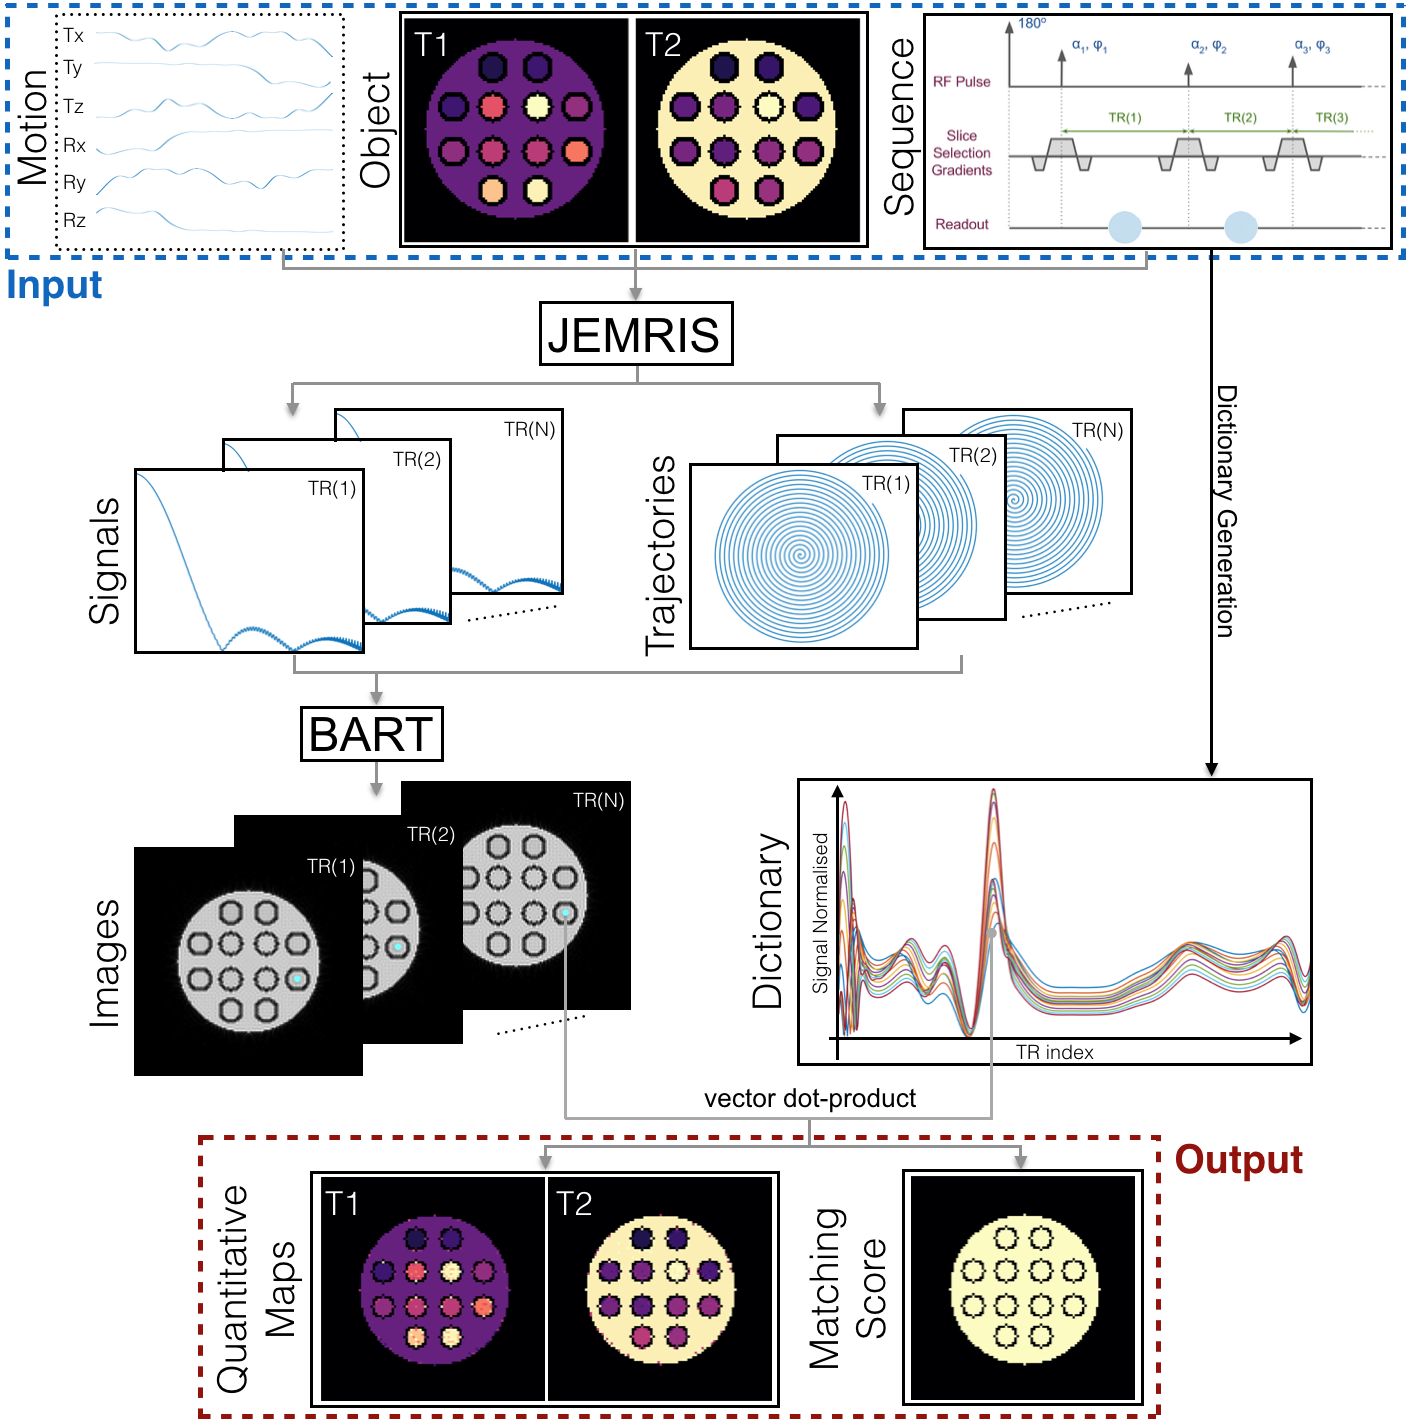
\includegraphics[angle=0,width=1\textwidth, keepaspectratio]{images/mrf/methodFramework}
    \caption{Image space simulation pipeline of a magnetic resonance fingerprinting experiment.
    The framework consists of three inputs: the digital phantom, the MR acquisition sequence and the motion trace. 
    The latter is shown here with dashed lines because it is an optional input parameter. 
    The open source MRI simulator JEMRIS is used to generate signals for each repetition period.
    Then, the BART toolbox is used to reconstruct the images.
    Separately, a dictionary of simulated signals is generated from first principles for a wide range of tissue properties.
    Finally, the quantitative maps are generated together with their corresponding pattern matching scores.}
    \label{fig:methodFramework}
\end{figure}

\hfill

The framework takes three inputs.
The first one is a geometric object which specifies the proton density and the $T_1$ and $T_2$ relaxation times at every spatial location.
The second is an inversion recovery rapid gradient-echo multi-pulse sequence with spiral readout (see Appendix \ref{chapterlabel2sec14}). 
For the dictionary generation part, I experimented with two types of sequences: \ac{bssfp} (see Appendix \ref{MRIBSSFP}) and \ac{fisp} (see Appendix \ref{MRIFISP}).
For the image space simulation part I have, so far, only simulated the \ac{bssfp} sequence.
The third input is the motion sequence where parameters for both translations and rotations can be specified.
These three inputs are then fed to JEMRIS which simulates the MR acquisition process and generates the signal for each repetition period of the multi-pulse sequence.
These signals, together with their corresponding k-space trajectory, are then fed into a software toolbox called BART \cite{Lustig2016} which reconstructs the images.
Separately, the same sequence is used to generate a database of signals, called `dictionary', for a wide range of relaxation parameters.

\hfill

The framework creates two outputs: the quantitative maps and the matching scores.
The former are created by first performing a voxel-wise pattern matching algorithm between all image space signals and all dictionary signals and then choosing the dictionary signal that gives the highest score as the most representative one for the voxel.
The latter are just the pattern matching scores showing how similar the two signals are.
More details related to the general MRF framework can be found in Appendix \ref{chapterlabel2sec22}.

\hfill

In the following sections I describe every part of our framework in more depth.
We start with the dictionary generation part as this is the first step in an MRF pipeline.
Next, I move on to explaining the image space simulations, together with the motion traces used for the experiments.
Finally, I explain the pattern matching algorithm used to create the quantitative maps.

\hfill

% % % % % % % % % % % % % % % % % % % % % % % % % % % % % % % % % % % % % % % % % % % % % % % % % % % % % % % % % % % % % % % % % % % % % % % % % % % % % % % % % % % % % % % % % % % % % % % % % % % % % % % % % % % % % % % % % % % % % % % % % % % % % % % % % % % % % % % % % % % % % % % % 
\subsection{Dictionary Generation}
\label{method:dictionary}

The first step in an MRF experiment is the creation of a dictionary of simulated signals for a wide variety of tissue properties.
This section presents an overview of the methods used for creating the database of signals for both a \ac{bssfp}-type sequence and a \ac{fisp}-type sequence.

\hfill

% \large \textbf{bSSFP Dictionary} \normalsize
\subsubsection{bSSFP Dictionary}

The \ac{bssfp} dictionary generation is based on the original implementation of the MRF sequence, where Ma et al. \cite{Ma2013} used an inversion-recovery balanced steady state free-precession sequence (see Figure~\ref{fig:sequencebSSFP}). 
The \ac{bssfp} sequence is a type of rapid multi-pulse gradient-echo pulse sequence. 
It is called `rapid' because the repetition time $T_R$ is shorter than both the longitudinal ($T_1$) and the transverse ($T_2$) relaxation times of most known tissue types.
Moreover, it uses balanced (fully rewound) gradients in every direction, thus effectively recovering the transverse magnetisation at the end of each $T_R$ period.

\hfill

\ac{bssfp} sequences are known to be highly sensitive to inhomogeneities in the main magnetic field. 
These inhomogeneities are caused by susceptibility variations or poor magnet shimming and give rise to `banding artifacts' in the final images \cite{Hargreaves2012}.
In spite of this, \ac{bssfp}-type sequences are used clinically today and are known commercially as: True-FISP, FIESTA, Balanced-FFE or True SSFP \cite{Hargreaves2012}.
These sequences are known to yield the highest signal among all the other rapid gradient-echo sequences and give a contrast of $T_2/T_1$ \cite{Scheffler2003}.

\begin{figure}[ht]
    \centering
    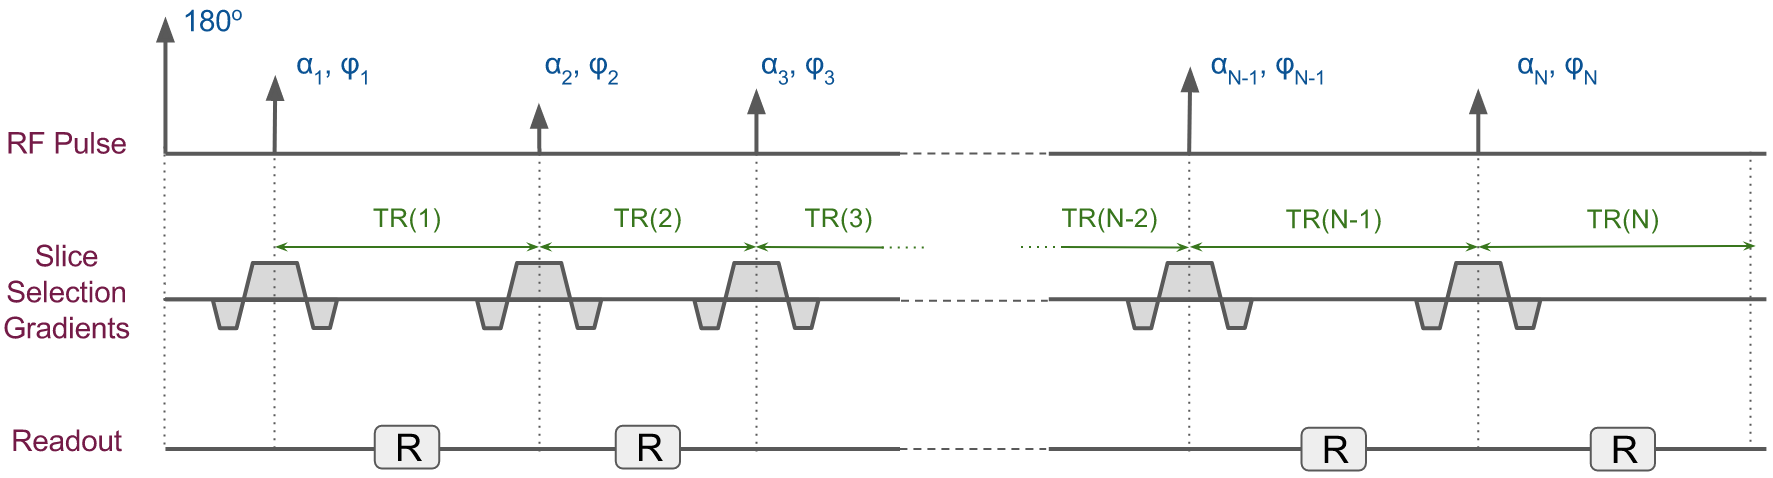
\includegraphics[angle=0,width=1\textwidth, keepaspectratio]{images/mrf/sequencebSSFP}
    \caption{The figure shows a simplified version of an IR-bSSFP sequence. 
    All gradients are fully balanced on every direction (they have a net moment of zero at the end of each repetition period) and readout is in the middle of each repetition period.}
    \label{fig:sequencebSSFP}
\end{figure}

\hfill

\large \textbf{Assumptions} \normalsize

To model the behaviour of a magnetisation vector with known relaxation times and proton density values in an MRF-\ac{bssfp} sequence, the following assumptions are made:

\begin{enumerate}
    \item The object for which I am modelling the magnetisation dynamics in the multi-pulse sequence is considered to be motionless.

    \item The effect of applying an RF pulse of flip angle $\alpha$ and phase angle $\phi$ was considered to be significantly shorter than the relaxation times $T_1$ and $T_2$ and was modelled as happening instantaneously.
    This allowed me to represent its effect as a rotation through the flip angle $\alpha$ about a chosen axis (e.g. the $x$-axis) and a change of coordinate system through the phase angle $\phi$ about the $z$-axis.
    % This is called the "hard pulse approximation" and is detailed in Appendix~\ref{background:rfpulse}.
    
    \item All gradients in this sequence are considered to be fully balanced, i.e. all the gradients on all axes have zero zeroth moment at the end of each repetition period.
    For this reason, I neglected the effect of gradients on the magnetisation vector.

\end{enumerate}

\clearpage

\large \textbf{Single Block Dynamics} \normalsize

In order to simulate the magnetisation dynamics in this multi-pulse sequence, 
%we first describe the effect of a single, arbitrarily chosen, $T_R$ block on a known magnetisation vector (see Figure~\ref{fig:sequencebSSFPOneBlock}).
I begin with the description of a single, arbitrarily chosen, $T_R$ block on a known magnetisation vector (see Figure~\ref{fig:sequencebSSFPOneBlock}).
The magnetisation vector immediately prior to the $i^{th}$ RF pulse is defined as:
\begin{equation}
    M^{-}_i \equiv \big[ M^-_{x_i} \, \,  M^-_{y_i} \, \, M^-_{z_i} \big]^T
\end{equation}
and immediately after the $i^{th}$ RF pulse as:
\begin{equation}
    M^{+}_i \equiv \big[ M^+_{x_i} \, \,  M^+_{y_i} \, \, M^+_{z_i} \big]^T
\end{equation}

\begin{figure}[ht]
    \centering
    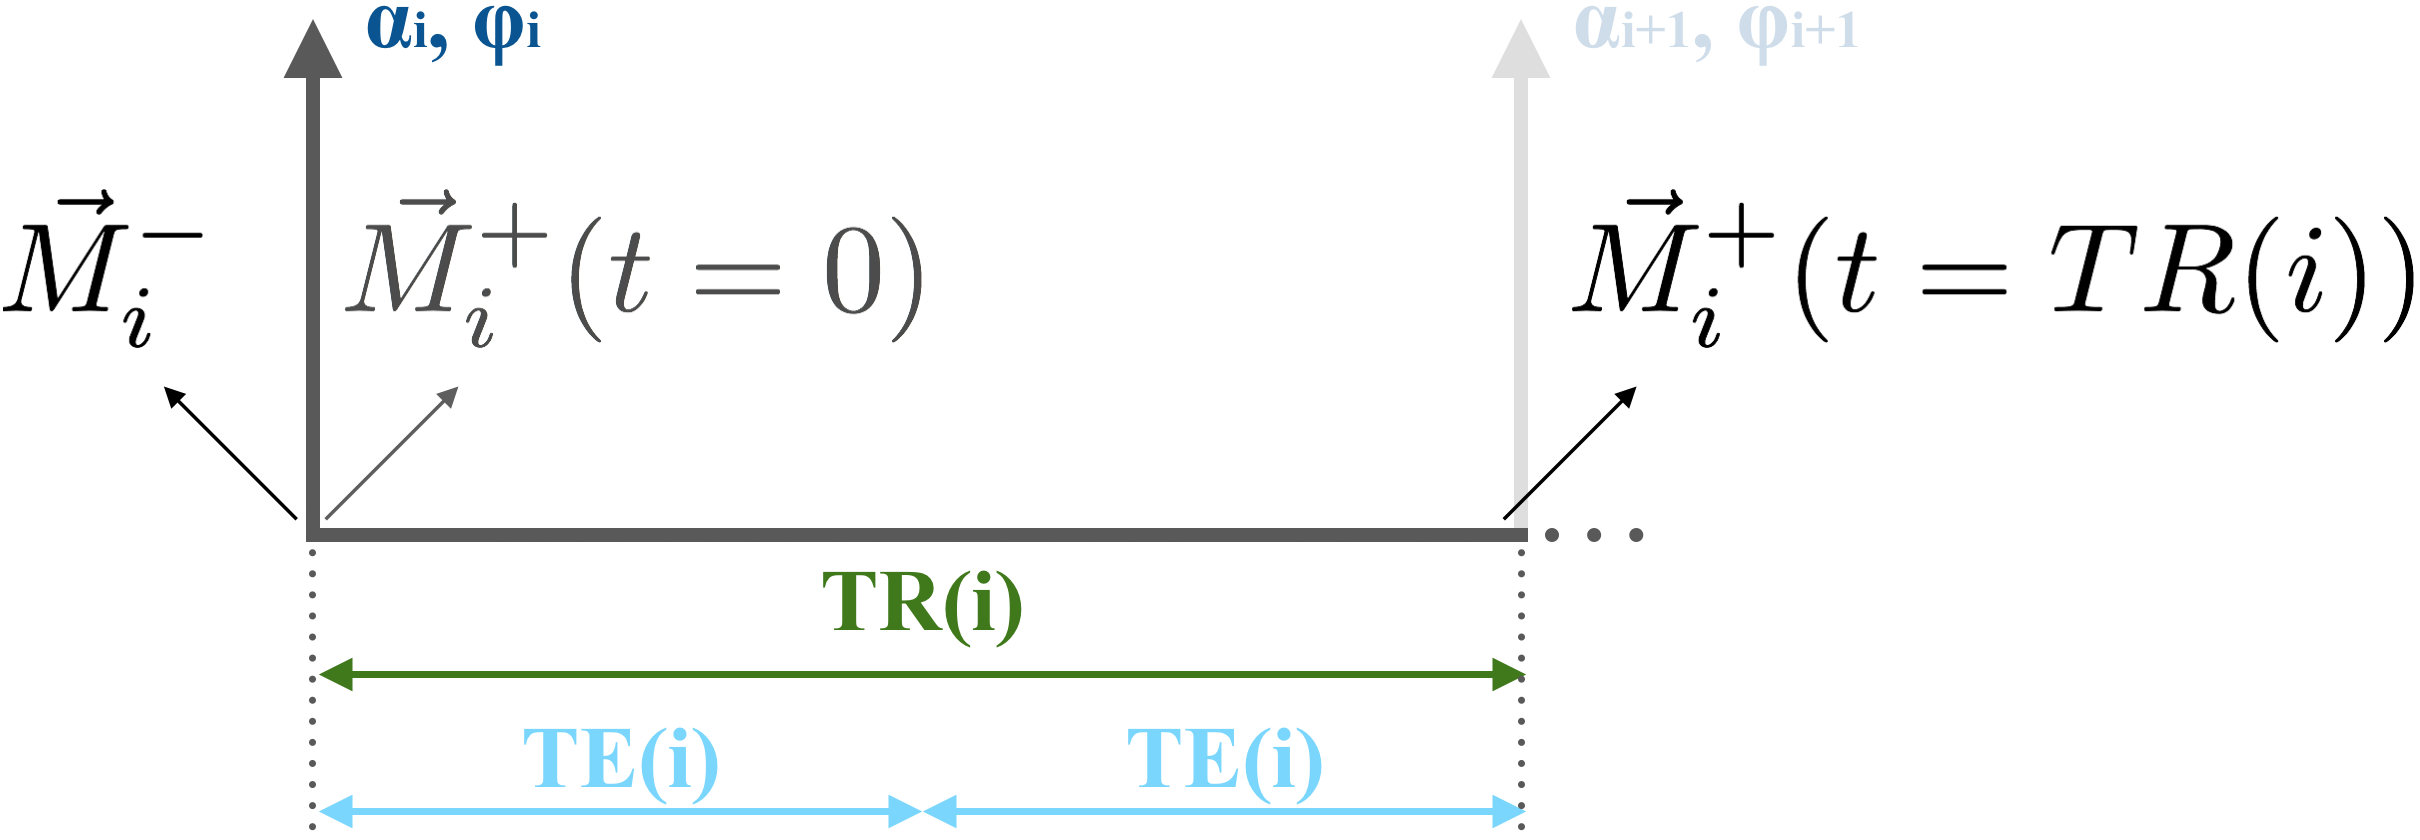
\includegraphics[angle=0,width=1\textwidth, keepaspectratio]{images/mrf/sequencebSSFPOneBlock}
    \caption{The figure shows a simplified version of an arbitrarily chosen repetition period block from the bSSFP sequence above.
    The magnetisation vector immediately prior to the $i^{th}$ RF pulse, i.e. $\vec{M}^-_i$, is the input to this block.
    The application of an RF pulse with flip angle $\alpha_i$ and phase angle $\phi_i$ on this magnetisation vector transforms it into $\vec{M}^+_i(t=0)$.
    Relaxation and off-resonance effects on this magnetisation vector transform it from $\vec{M}^+_i(t=0)$ into $\vec{M}^+_i(t=T_R(i))$, the output of this block.
    % The second magnetisation vector is formed as a result of the application of the $i^{th}$ RF pulse with flip angle $\alpha_i$ and phase angle $\phi_i$ on the $\vec{M}^-_i$ vector.
    % Similarly, $\vec{M}^-_{i+1}$ and $\vec{M}^+_{i+1}$ are the magnetisation vectors immediately before and after the $(i+1)^{th}$ RF pulse.
    %The relationship between $\vec{M}^+_{i}$ and $\vec{M}^-_{i+1}$ is given by: $ \vec{M}^-_{i+1} = \vec{M}^+_{i}(t = TR(i))$, where $t \in [0, TR(i)]$ 
    }
    \label{fig:sequencebSSFPOneBlock}
\end{figure}

\textbf{RF Pulse.} 
The effect of an instantaneous RF pulse with flip angle $\alpha_i$ and phase angle $\phi_i$ links the two vectors through rotation matrices (see Assumption 2 and Appendix~\ref{app:rfpulse}):

\begin{equation}\label{eq:rfpulseequationbssfp}
    \begin{split}
        M^{+}_i & = R_{z}(\phi_i) R_{x}(-\alpha_i) R_{z}(-\phi_i) M^{-}_i \\
        \text{where:}         & \\
        & R_x(\alpha) = 
            \begin{bmatrix}
                1 &       0     &       0      \\
                0 & \cos(\alpha) & -\sin(\alpha) \\
                0 & \sin(\alpha) & \phantom{-}\cos(\alpha)
            \end{bmatrix} \\
        & R_z(\phi) = 
            \begin{bmatrix}
    	        \cos(\phi) & -\sin(\phi) & 0 \\
                \sin(\phi) & \phantom{-}\cos(\phi) & 0 \\
                    0   &      0     & 1
            \end{bmatrix}
    \end{split}
\end{equation}

\hfill

\textbf{Relaxation and off-resonance.} 
Next, the magnetisation vector will begin the process of returning to its equilibrium state.
This phenomenon is governed by the $T_1$ and $T_2$ relaxation times of the tissue being modelled, as well as the off-resonance effects caused by static field inhomogeneities $\Delta B$.
Using matrix notation, this becomes (more details in Appendix~\ref{app:matrixbloch}):
%, as well as the off-resonance effects caused by static field inhomogeneities $\Delta B$.
%  can be described using matrix notation (more details in Appendix~\ref{app:matrixbloch}).
% In the rotating reference frame (after demodulating with the Larmor frequency $\omega_0$), this phenomenon can be described as:
\begin{equation}\label{eq:multiblockdyn}
    M^{+}_i (t)  = D(t) R_z(-\omega t) M^{+}_i (0) + C(t)
\end{equation}
where
\begin{equation}\label{eq:dmatrix}
    \begin{split}
        D ( t ) &= \left[
        \begin{array}{c c c}
              E_2(t) &     0      &     0 \\
               0     &   E_2(t)   &     0 \\
               0     &     0      &   E_1(t)
        \end{array}
        \right] \, \, \text{, } \, 
        C ( t ) = \left[
        \begin{array}{c}
            0 \\
            0 \\
        M_0(1 - E_1(t))
        \end{array}
        \right] \\
        E_1(t) &\equiv e^{-t/T_1} \text{, } E_2(t) \equiv e^{-t/T_2} \text{, } \omega = \gamma \lvert \vec{B}_0 + \Delta \vec{B} \rvert = \omega_0 + \Delta \omega \text{ and } t \in [0, T_R(i)]
    \end{split}
\end{equation}
%\text{ (see Appendix~\ref{eq:omegaEffects})}
%and where $E_1(t) \equiv e^{-t/T_1}$, $E_2(t) \equiv e^{-t/T_2}$, $\omega = \gamma \lvert \vec{B}_0 + \Delta \vec{B} \rvert = \omega_0 + \Delta \omega$ (see Appendix~\ref{eq:omegaEffects}) and
%$t \in [0, T_R(i)]$.
%After the RF pulse, the magnetisation vector will try and return to its thermal equilibrium.
%To capture the dynamics of the magnetisation vector I use the solution to the Bloch equation in matrix form (as presented in Appendix~\ref{app:matrixbloch}).
%For completion 

\hfill

In the rotating reference frame (after demodulating with the Larmor frequency $\omega_0$) equation \ref{eq:multiblockdyn} becomes:
\begin{equation}\label{eq:multiblockdynfinal}
    M^{+}_i (t)  = D(t) R_z(-\beta(t)) M^{+}_i (0) + C(t)
\end{equation}
where I introduced the precession angle of the transverse magnetization components during each repetion block as: $\beta(t) = \gamma \Delta B t = \Delta \omega t = 2\pi \Delta \nu t$. 

\hfill

At the end of the $i^{th}$ repetition block the magnetisation vector becomes:
\begin{equation}
    M^{+}_{i}(T_R(i)) = D\big(T_R(i)\big) R_z\big(-\beta(T_R(i))\big) \underbrace{\big( R_{z}(\phi_i) R_{x}(-\alpha_i) R_{z}(-\phi_i) M^{-}_i \big)}_{M_i^+(0)} + C\big(T_R(i)\big)
\end{equation}

% \textbf{Relaxation.} 
% Next, the magnetisation vector will begin the process of returning to its equilibrium state.
% This phenomenon is governed by the $T_1$ and $T_2$ relaxation times of the tissue being modelled and can be described using matrix notation (more details in Appendix~\ref{chapterlabel2sec1Bloch}).
% In the rotating reference frame (after demodulating with the Larmor frequency $\omega_0$), this phenomenon can be described as:

% \begin{equation}
%     M^{+}_i (t)  = D(t) M^{+}_i (0) + C(t)
% \end{equation}
% where
% \begin{equation}\label{eq:dmatrix}
%     D ( t ) = \left[
%     \begin{array}{c c c}
%           E_2(t) &     0      &     0 \\
%           0      & E_2(t) &     0 \\
%           0      &     0      & E_1(t)
%     \end{array}
%     \right] \, \, \text{,  } \, 
%     C ( t ) = \left[
%     \begin{array}{c}
%         0 \\
%         0 \\
%     M_0(1 - E_1(t))
%     \end{array}
%     \right]
% \end{equation}

% and where $E_1(t) \equiv e^{-t/T_1}$, $E_2(t) \equiv e^{-t/T_2}$ and
% $t \in [0, T_R(i)]$.

% \hfill

% \textbf{Off-resonance.} 
% In the case where static field inhomogeneities $\Delta B$ are present, the phase of the magnetisation vector will change over a given repetition time period. 
% This phase is determined by $\beta(t) = \gamma \Delta B t = \Delta \omega t = 2\pi \Delta \nu t$ during any $T_R$ block.
% To model the behaviour of phase accrual, an instantaneous rotation about the $z$ axis of the magnetisation vector is used.
% This can be mathematically represented as:

% \begin{equation}
%     M^{+}_i (t)  = R_z(\beta(t)) M^{+}_i (0)
% \end{equation}

% where the rotation matrix $R_z$ has been previously described.
% %and $\beta(t) = 2\pi \, \, \Delta \nu \, \, t$ is the accumulated phase due to off-resonance frequency $\Delta \nu$ at time $t$ during the $i^{th}$ repetition period. 
% %Again, we can choose $t = T_{E_i}$ or $t = T_{R_i}$ to calculate the magnetisation vector components at the echo time or at the end of a repetition period, respectively.

\hfill

\large \textbf{Multiple Blocks Dynamics} \normalsize

The extension from single block simulations to multi-pulse simulations is straightforward.
By setting $M^{-}_1 = M_0 \hat{x}$,
%and iterating through $i \in [1, N_{pulses}]$, 
the magnetisation vector at the end of the $i^{th}$ repetition period can be calculated from the magnetisation vector immediately prior to that block. 
This process is repeated for every $i \in [1, N_{pulses}]$ with the sequence properties corresponding to that block.
% \begin{equation}
%     M^{-}_{i+1} = D\big(T_R(i)\big) R_z\big(\beta(T_R(i))\big) \big( R_{z}(\phi_i) R_{x}(-\alpha_i) R_{z}(-\phi_i) M^{-}_i \big) + C\big(T_R(i)\big)
% \end{equation}

\hfill

% The magnetisation vector components at echo time can be calculated for every $T_R$ block and the signal for a single tissue type in a multi-pulse sequence can be retrieved.
% These events can now be linked together to calculate the magnetisation vector at time $t$ after the $i^{th}$ RF pulse:

% These three events, RF pulse, relaxation and off-resonance effects, fully describe the magnetisation dynamics of a spin ensemble with equilibrium magnetisation $M_0$, relaxation constants $T_1$ and $T_2$, and with off-resonance frequency $\Delta \nu$.
% These events can now be linked together to calculate the magnetisation vector at time $t$ after the $i^{th}$ RF pulse:
% \begin{equation}
%     M^{+}_i (t) = D(t) R_z(\beta(t)) \big( R_{z}(\phi_i) R_{x}(-\alpha_i) R_{z}(-\phi_i) M^{-}_i \big) + C(t)
% \end{equation}

\large \textbf{Dictionary} \normalsize

In order to create a dictionary of signals in a multi-pulse IR-\ac{bssfp} sequence, the previously described process is repeated for a range of tissue properties.
More specifically, every signal is associated with a `tissue tuple':
$(T_{1_j}, T_{2_j}, \Delta \nu_{j})$, with $j \in [1, M]$, where $M$ is the total number of tuples.
Hence, the dictionary is creating a function relationship between tissue properties and signals.

\hfill

The dictionary was created in MATLAB using a vectorised version of the previously described process.
The speed of this method comes from the fact that the magnetisation vector components of all tissue types are calculated simultaneously, for every $T_R$ period.
For this, I start by defining a $3 \times M$ matrix for the $M_x, \, M_y, \, M_z$ components of the magnetisation vector for all $M$ tissue types immediately before the $i^{th}$ RF Pulse:
\begin{equation}
    M^{-}_i = 
    \begin{bmatrix}
        M_{ix_1} & M_{ix_2} & \dots & M_{ix_M} \\
        M_{iy_1} & M_{iy_2} & \dots & M_{iy_M} \\
        M_{iz_1} & M_{iz_2} & \dots & M_{iz_M}
    \end{bmatrix}
\end{equation}

To flip the magnetisation vectors of all the tissue types, the RF pulse matrix is precomputed for the current repetition period:
\begin{equation}
        R_{\phi_i}(\alpha_i) = R_{z}(\phi_i) R_{x}(-\alpha_i) R_{z}(-\phi_i)
\end{equation}
and then applied to the previously defined $3 \times M$ matrix of magnetisation vector components:
\begin{equation}
    M^{+}_i(0) = R_{\phi_i}(\alpha_i) \, \, M^{-}_i
\end{equation}

For the off-resonance effects, the process is split in two.
Two $3 \times M$ matrices are created to represent the effect of rotation about the z-axis for all possible $\beta_j(t) = 2\pi \Delta \nu_j \, t$ \big(with $j \in [1, M]$ \big) off-resonance angles.
Mathematically, this is given by:
\begin{equation}
    M^{+}_i (t) = R_{\Delta \nu_1}(t) \, \odot \, M^{+}_i(0) + R_{\Delta \nu_2}(t)  \, \odot \, M^{+}_i(0)^{(p)}
\end{equation}

where $\odot$ denotes component-wise multiplication, and:

\begin{equation}
    R_{\Delta \nu_1}(t)  = \begin{bmatrix} \phantom{-}\cos(\beta_{1}(t) ) & \phantom{-}\cos(\beta_{2}(t) ) & \dots & \phantom{-}\cos(\beta_{M}(t) ) \\
    \phantom{-}\cos(\beta_{1}(t) ) & \phantom{-}\cos(\beta_{2}(t) ) & \dots & \phantom{-}\cos(\beta_{M}(t) ) \\
    1    &        1   & \dots &  1
    \end{bmatrix}
\end{equation}

\begin{equation}
    R_{\Delta \nu_2}(t)  = \begin{bmatrix} -\sin(\beta_{1}(t) ) & -\sin(\beta_{2}(t) ) & \dots & -\sin(\beta_{M}(t) ) \\
    \phantom{-}\sin(\beta_{1}(t) ) & \phantom{-}\sin(\beta_{2}(t) ) & \dots & \phantom{-}\sin(\beta_{M}(t) ) \\
    0     &      0      & \dots &      0
    \end{bmatrix}
\end{equation}

\begin{equation}
\begin{split}
    M^{+}_i(0) = &
    \begin{bmatrix}
        M^{+}_{ix_1}(0) & M^{+}_{ix_2}(0) & \dots & M^{+}_{ix_M}(0) \\
        M^{+}_{iy_1}(0) & M^{+}_{iy_2}(0) & \dots & M^{+}_{iy_M}(0) \\
        M^{+}_{iz_1}(0) & M^{+}_{iz_2}(0) & \dots & M^{+}_{iz_M}(0)
    \end{bmatrix} \\
    = & \, \, R_{\phi_i}(\alpha_i) \, \, M^{-}_i \text{ (as previously defined)}
\end{split}
\end{equation}

\begin{equation}
\begin{split}
    M^{+}_i(0)^{(p)} = &
    \begin{bmatrix}
        M^{+}_{iy_1}(0) & M^{+}_{iy_2}(0) & \dots & M^{+}_{iy_M}(0) \\
        M^{+}_{ix_1}(0) & M^{+}_{ix_2}(0) & \dots & M^{+}_{ix_M}(0) \\
        M^{+}_{iz_1}(0) & M^{+}_{iz_2}(0) & \dots & M^{+}_{iz_M}(0)
    \end{bmatrix} \\
    & \text{ (Obs: lines 1 and 2 have been permuted)}
\end{split}
\end{equation}

For the relaxation effects, two $3 \times M$ matrices are built to account for all M combinations of $T_1$ and $T_2$ decay rates:
\begin{equation}
    M^{+}_i(t) = D(t)  \, \odot \, M^{+}_i(0) + C(t) 
\end{equation}

where, again, $\odot$ denotes component-wise multiplication, and:

\begin{equation}
    D(t)  = 
    \begin{bmatrix}
        E_{2_1}(t)  & E_{2_2}(t)  & \dots & E_{2_M}(t)  \\
        E_{2_1}(t)  & E_{2_2}(t)  & \dots & E_{2_M}(t)  \\
        E_{1_1}(t)  & E_{1_2}(t)  & \dots & E_{1_M}(t)  
    \end{bmatrix}
\end{equation}

and

\begin{equation}
    C(t)  = 
    \begin{bmatrix}
        0 & 0 & \dots & 0 \\
        0 & 0 & \dots & 0 \\
        1 - E_{1_1}(t)  & 1- E_{1_2}(t)  & \dots & 1- E_{1_M}(t)  
    \end{bmatrix} 
\end{equation}

where $E_{1_j}(t) \equiv e^{-t/T_{1_j}}$ and $E_{2_j}(t) \equiv e^{-t/T_{2_j}}$, with $j \in [1, M]$.

\hfill 

This process is then repeated, in order, for all repetition times in the sequence.
At the end, a dictionary of M signals, each with N time points is constructed.
For completion, I store all 3 components of the magnetic moment vectors, thus having an $M \times N \times 3$ dictionary matrix.
Pseudocode for the created algorithms can be found in Appendix~\ref{appendixlabel1}.

\hfill

\subsubsection{FISP Dictionary} 
\label{method:fispdictionary}

The \ac{fisp} dictionary generation is based on a more recent implementation of the MRF sequence, where Jiang et al. \cite{Jiang2015} used an inversion-recovery fast imaging with steady-state precession sequence (see Figure~\ref{fig:sequenceFISP}).
Similar to \ac{bssfp}, \ac{fisp} is also a type of rapid multi-pulse gradient-echo sequence.
However, in contrast with the previous sequence, \ac{fisp} uses an unbalanced gradient in one or multiple gradient directions, thus `spoiling' the transverse magnetization prior to the next RF pulse \cite{Hargreaves2012}.
Gradient spoiling does not effectively null the transverse magnetisation, so then both the longitudinal and the transverse magnetisation components will contribute to the signal in the next cycle.

\begin{figure}[ht]
    \centering
    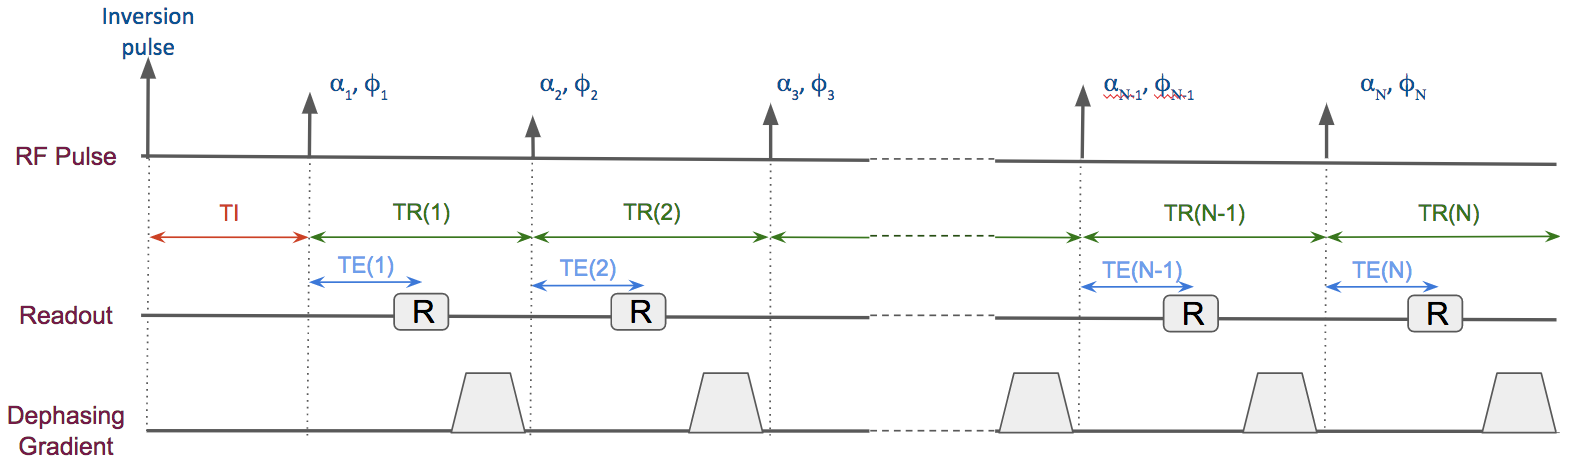
\includegraphics[angle=0,width=1\textwidth, keepaspectratio]{images/mrf/sequenceFISP}
    \caption{The figure shows a simplified version of an inversion recovery fast imaging with steady state precession sequence. 
    Unlike \ac{bssfp}, a \ac{fisp} sequence contains an unbalanced `spoiler' gradient in each each repetition period.
    Otherwise, all other gradients are fully balanced in every direction.
    Here, $N$ represents the total number of RF pulses.}
    \label{fig:sequenceFISP}
\end{figure}

\hfill

\ac{fisp}-type sequences are used in MR imaging due to their fast imaging characteristics and their immunity to the banding artefacts commonly seen in fully balanced steady state sequences. 
%As with \ac{bssfp}, the signal in these types of sequences is a function of $T_2/T_1$ \cite{Hargreaves2012}. 
%\ac{fisp}-type sequence yield a lower signal than in \ac{bssfp} and 
Commercially, \ac{fisp}-type sequences are known as: FE, FFE, GRASS, GRE, \ac{fisp}, FAST \cite{Hargreaves2012}.
These sequences are known to yield a lower signal magnitude than balanced sequences, while keeping a similar signal contrast of $T_2/T_1$ \cite{Hargreaves2012}.

\hfill

\large \textbf{Assumptions} \normalsize

In order to simulate the behaviour of a magnetisation vector with known relaxation times and proton density values in an MRF-\ac{fisp} sequence, single isochromat Bloch equations are no longer applicable.
Due to the presence of a strong dephasing gradient and repetition times shorter than the transverse relaxations of most tissue types \big($T_R \leq T_2$\big), the transverse magnetisation will not be destroyed, but completely dephased across a voxel.
To model this, an algorithm called the \ac{epg} \cite{Hennig1988} \cite{Hennig1991} was used.

\hfill 

The \ac{epg} formalism \cite{Hennig1988} \cite{Hennig1991} \cite{Weigel2015} is used to simulate signals obtained from a wide variety of MRI pulse sequences \cite{Malik2017}.
% EPG has been used for a variety of applications such as:
% characterization of RF spoiling in gradient echo sequences (4,5), 
% analysis of echo amplitudes in turbo spin echo (TSE) sequences (6–9), 
% diffusion effects (12), and 
% characterizing signal evolution in sequences used for relaxometry (13–16).
Similar to the Bloch equations approach, \ac{epg} characterizes a given sequence through the effects of RF pulses, relaxation constants, and dephasing due to gradients or inhomogeneities in the main magnetic field.
% However, in this formalism large groups of spins are represented as a compact Fourier basis set of $F_k$ and $Z_k$ coefficients.
% However, unlike the previous approach, EPG describes a spin system as a discrete set of phase states (or, `configuration states') \cite{Hennig1988}.
% These states appear as a consequence of 
To model the behaviour of a spin ensemble 
%with known relaxation times and proton density values 
in a single-voxel MRF-\ac{fisp} sequence, the following assumptions were made:
% This algorithm works under certain assumptions which we enumerate here:

%Bloch equations can be used, but a large number of isochromats needs to be simulated to achieve accuracy.
% For this, a different approach was used, called the Extended Phase Graph formalism \cite{Hennig1988} \cite{Hennig1991}.

\begin{enumerate}

    \item The object for which I am modelling the magnetisation dynamics in the multi-pulse sequence is considered to be motionless.

    \item The tissue being modelled is represented by a single voxel with uniform density of magnetisation, characterised by a single set of relaxation parameters and spin density values.
    
    \item The 1D voxel has dimension in the same direction as the applied gradient, where one edge of the voxel is considered to be the `isocentre'.
    Gradient areas are quantized into units that give a phase twist of one cycle ($2\pi$), such that the amount of dephasing induced by one application of the gradient is ranging from $[0, 2\pi]$. 
    Moreover, for improved visualisation and pictorial understanding, I presume that the gradient is in the z-direction.

    \item The `spoiling' gradient used in this sequence has the same amplitude and duration in every repetition period.
    Thus, the gradient induces the same amount of dephasing across the voxel during each of its applications.
    %a fixed time period $\Delta t$ at the end of each repetition period.
    
    \item The effect of applying an RF pulse of flip angle $\alpha$ and phase angle $\phi$ was considered to be significantly shorter than the relaxation times $T_1$ and $T_2$ and was modelled as happening instantaneously.
    This allowed me to represent its effect as a rotation through the flip angle $\alpha$ about a chosen axis (e.g. the $x$-axis) and a change of coordinate system through the phase angle $\phi$ about the $z$-axis.
    This is called the hard pulse approximation and is detailed in Appendix~\ref{background:rfpulse}.

\end{enumerate}

\hfill

\large \textbf{Extended Phase Graph Formalism} \normalsize

In this section explains the main ingredients behind the \ac{epg} formalism, starting from a simple example of a fully relaxed spin system.
The extended phase graph formalism is a tool for understanding MR signal progression and echo formation in a wide variety of MR sequences.
In \ac{epg}, the full state of the signal across a voxel is represented by a small number of coefficients.
These coefficients encode the distribution of the isochromat population into different Fourier basis functions.
These basis functions are either a set of transverse basis functions called $\bm{F_k}$ and $\bm{F_{-k}}$ or longitudinal basis functions called $\bm{Z_k}$.

\hfill

Mathematically, these configuration states are related to
%form a Fourier pair with 
the complex transverse magnetisation $M_{+}$ and longitudinal magnetisation $M_z$ \cite{Hennig1991} through:
\begin{equation}
\begin{split}
    F_{k}  & = \int_0^1 M_{+}(z) e^{- i 2\pi k z} dz \\ %& \Longleftrightarrow M_{+}(z) = \int_{- \infty}^{+ \infty}  F_{k} e^{+ i 2\pi k z} dk \\
    F_{-k} & = \int_0^1 M_{-}(z) e^{- i 2\pi k z} dz \\ %& \Longleftrightarrow M_{-}(z) = \int_{- \infty}^{+ \infty}  F_{-k} e^{+ i 2\pi k z} dk \\
    Z_{k} & = \int_0^1 M_{z}(z) e^{- i 2\pi k z} dz %& \Longleftrightarrow M_{z}(z) = \int_{- \infty}^{+ \infty} Z_{k} e^{+ i 2\pi k z} dk
\end{split}    
\end{equation}
where z is the voxel dimension and is in the $[0,1]$ range (without loss of generality) and $M_+ = (M_-)^*$.
The $F_{k}$ and $F_{-k}$ states can be thought of as a two counter-rotating isochromat populations \cite{Brown}.

\hfill

\textbf{The $\bm{F_0}$ and $\bm{Z_0}$ configuration states}

% In this section we explain the main ingredients behind the EPG formalism, starting from a simple example of a fully relaxed spin system.
%In order to model the behaviour of a spin ensemble with known relaxation times and proton density values in a single-voxel MRF-\ac{fisp} sequence, 
%In order to simulate the magnetisation dynamics in this multi-pulse sequence, 
%we begin with the description of a single $T_R$ block.
%In order to 
% To simplify things even further, we begin with the thermal equilibrium case, where the spin ensemble is fully relaxed and the magnetic moment vectors have the same direction as the main magnetic field (here considered to be $\hat{z}$).
At thermal equilibrium, an isochromat ensemble is fully relaxed and the magnetic moment vectors have the same direction as the main magnetic field (here considered to be $\hat{z}$).
This state in which the spin system is initially found is called a $\bm{Z_0}$ configuration \cite{Weigel2015} \cite{Scheffler1999} \cite{Hennig1991}.
The coefficient for this state is equal to $\bm{1}$ as the entire population of the imaginary spin ensemble is found in this configuration.
Pictorially, the $\bm{Z_0}$ state is shown in Figure~\ref{fig:Z0F0states} a) where I chose to represent 100 uniformly distributed isochromats along the voxel dimension.

\hfill

The application of an instantaneous $\pi/2$ excitation pulse on this configuration has the effect of `flipping' the entire isochromat ensemble in the transverse plane.
This new configuration is known as the $\bm{F_0}$ state \cite{Weigel2015} \cite{Scheffler1999} \cite{Hennig1991} and is graphically shown in Figure~\ref{fig:Z0F0states} b).
The $\bm{F_0}$ configuration is an important concept in the \ac{epg} formalism as it represents coherent transverse magnetisation and it is the cause of echo generation.
% 
% \hfill
% 
% The isochromat ensemble can `flip' back and forth between the two states by the application of the same instantaneous $\pi/2$ pulse.

\begin{figure}[H]
    \centering
    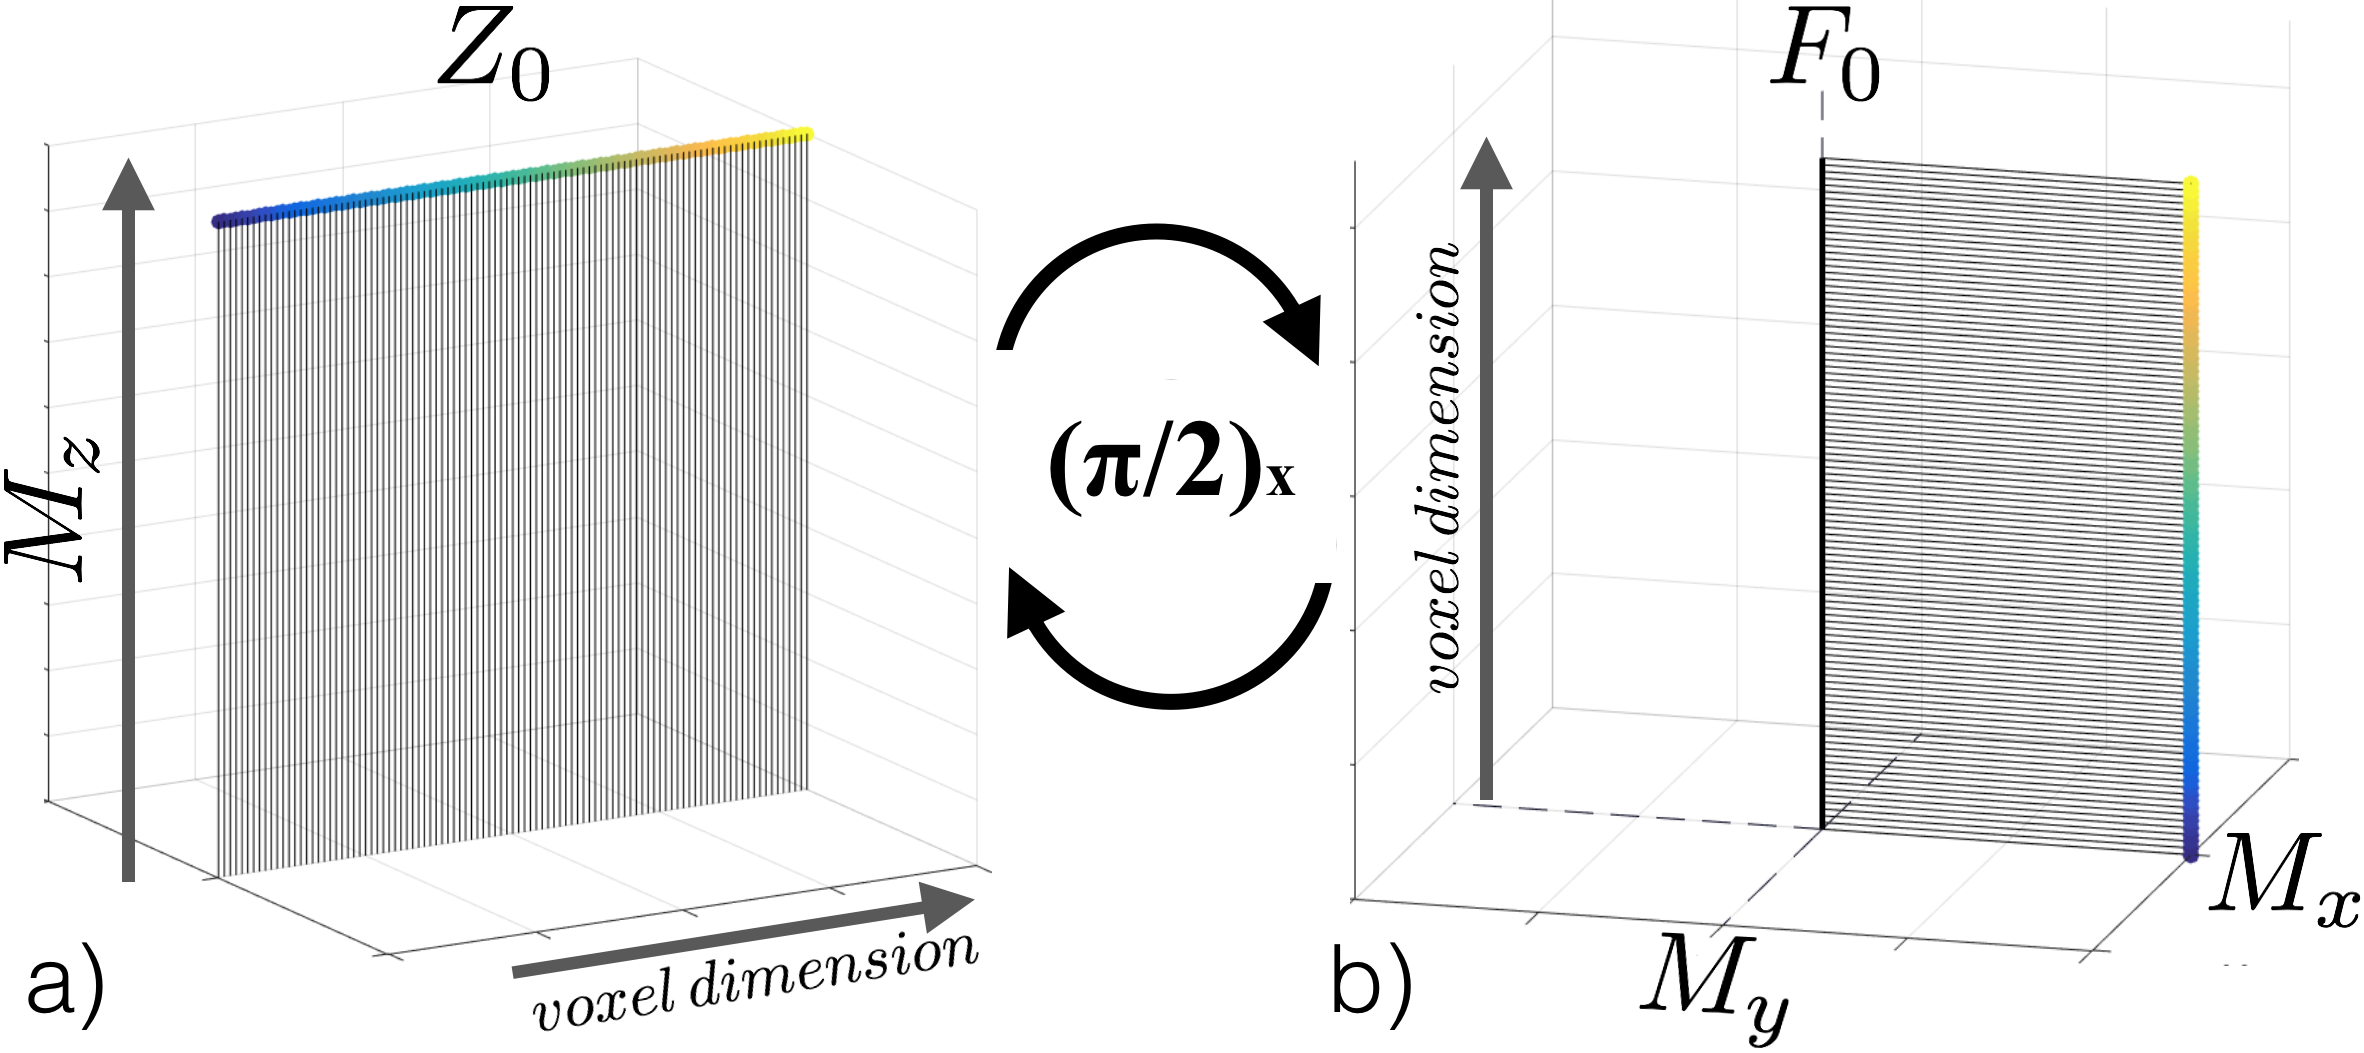
\includegraphics[angle=0,width=0.65\textwidth, keepaspectratio]{images/mrf/Z0F0states}
    \caption{The figure shows a pictorial representation of a single 1D voxel with uniform density of magnetisation.
    a) $\bm{Z_0}$ is a configuration in which the isochromat ensemble is characterised by spins lying along $M_z$.
    b) $\bm{F_0}$ is a configuration in which the isochromat ensemble is characterised by coherent transverse magnetisation.
    An instantaneous $\pi/2$ excitation pulse can `flip' the isochromat ensemble back and forth between the two states.
    It is important to note that a $(\pi/2)_x$ RF pulse applied on the $\bm{F_0}$ state will cause the isochromat ensemble to be pointing in the $- \hat{z}$ direction instead of the $+ \hat{z}$ direction it was initially found.
    However, this is still considered a $\bm{Z_0}$ configuration.
    }
    \label{fig:Z0F0states}
\end{figure}


\begin{figure}[H]
    \centering
    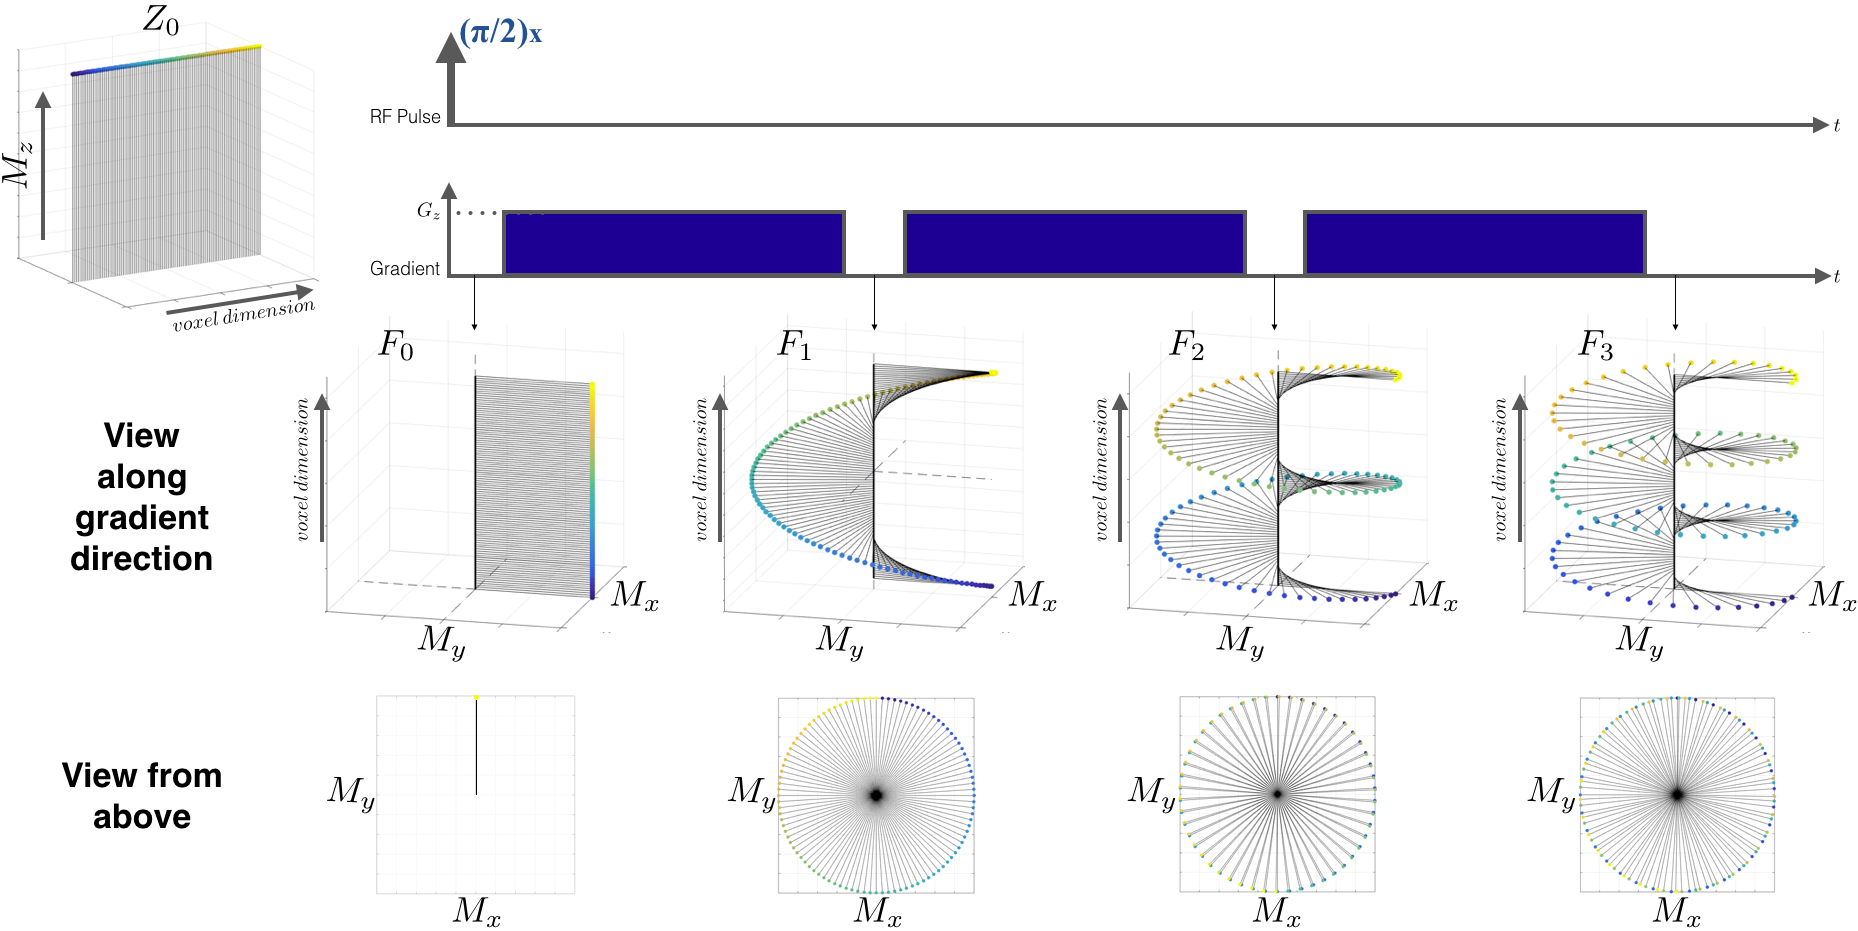
\includegraphics[angle=90,width=0.7\textwidth, keepaspectratio]{images/mrf/effectOfGradsEPG}
    \caption{Pictorial representation of an isochromat ensemble experiencing an ideal instantaneous $(\pi/2)_x$ RF pulse and dephasing induced by a gradient.
    This spin system is found in a 1D voxel whose dimension in along the same direction as the applied gradient (here, the $\hat{z}$ direction is considered) and which is positioned such that one edge of the voxel is at the `isocentre'. The isochromats found at the opposite edge accrue a phase of $2\pi$ after the application of this gradient.
    Every time the gradient is applied the spin system dephases further into a new configuration here represented as discrete states: $\bm{F_k}$.}
    \label{fig:effectOfGradsEPG}
\end{figure}

% % % % % % % % % % % % % % % % % % % % 
\textbf{The effect of a constant gradient on the isochromat ensemble} 

The application of a constant gradient introduces a linearly position-dependent off-resonance Larmor frequency on the isochromat ensemble along its axis (which is the same as the voxel dimension, as stated in the assumptions).
This can be seen in Figure~\ref{fig:effectOfGradsEPG} where after the first application of the gradient the spin system is now dephased.
This dephased configuration can be conceptually represented as an evenly distributed collection of magnetisation vectors called $\bm{F_1}$ \cite{Hennig1988} \cite{Scheffler1999}, where $\bm{k=1}$ represents one cycle of phase.
% Let us now introduce a dephasing gradient in the $\hat{z}$ direction (the 1D voxel's direction) that obeys the assumptions we previously described.
% This gradient induces phase accrual on the isochromat ensemble such that the isochromat found at one edge of the voxel is positioned at the `isocentre', while the isochromat found at the opposite edge experiences $2\pi$ dephasing.
% In fact, the off-resonance frequency increases linearly with the distance from the assumed `isocentre'.

\hfill

Each further application of the gradient increases the amount of dephasing experienced by the spin system with multiples of $2\pi$.
This can be seen in Figure~\ref{fig:effectOfGradsEPG} where each new application of the gradient `shifts' the spin system into a different configuration state.
These dephased configuration states are called $\bm{F_k}$, where $k$ represents the amount of $2\pi$ dephasing experienced by the spin ensemble.

\hfill

% % % % % % % % % % % % % % % % % % % % 
\textbf{The effect of an RF pulse on the isochromat ensemble} 

The application of an RF pulse of arbitrary flip angle $\alpha$ and phase angle $\phi$ on a dephased isochromat ensemble mixes the populations of spins among configurations.
This effect is best explained through equation \ref{eq:rfpulseequationbssfp}, which says that the magnetisation vectors immediately after the RF pulse are related to those immediately before the RF pulse through a rotation matrix (relaxation effects are neglected as the RF pulse is assumed to be instantaneous).
For completion, I rewrite equation \ref{eq:rfpulseequationbssfp} here:

\begin{equation}
    \begin{bmatrix} 
    M_x \\
    M_y \\
    M_z
    \end{bmatrix}^+ = 
        R_{\phi}(\alpha)
    \begin{bmatrix} 
    M_x \\
    M_y \\
    M_z
    \end{bmatrix}^-
\end{equation}
where, as before, superscript $+$ denotes `immediately after RF pulse' and superscript $-$ denotes 'immediately before RF pulse'.

\hfill

In complex notation, where $M_+ \equiv M_x + i M_y$,  $M_- \equiv M_x - i M_y$ and $M_- = (M_+)^*$ this becomes:

\begin{equation}\label{eq:magnbeforestates}
    \begin{bmatrix} 
    M_+ \\
    M_- \\
    M_z
    \end{bmatrix}^+ = 
        T_{\phi}(\alpha)
    \begin{bmatrix} 
    M_+ \\
    M_- \\
    M_z
    \end{bmatrix}^-
\end{equation}
where 
\begin{equation}\label{eq:woessnerFn2}
    T_{\phi}(\alpha) = 
    \begin{bmatrix}
        cos^2(\alpha/2) & e^{2i\phi} sin^2(\alpha/2) & - i e^{i \phi} sin(\alpha) \\
        e^{-2i\phi} sin^2(\alpha/2) & cos^2(\alpha/2) & i e^{-i \phi} sin(\alpha) \\
        - i/2 e^{-i \phi} sin(\alpha) & i/2 e^{i \phi} sin(\alpha) & cos \alpha
    \end{bmatrix}
\end{equation}

\hfill

% A completely dephased isochromat ensemble is rotated through an angle by the applied instantaneous RF pulse.
% This is seen in Figure~\ref{fig:RFpulseeffect} where we chose $\phi = 0$.

% \begin{figure}[ht]
%     \centering
%     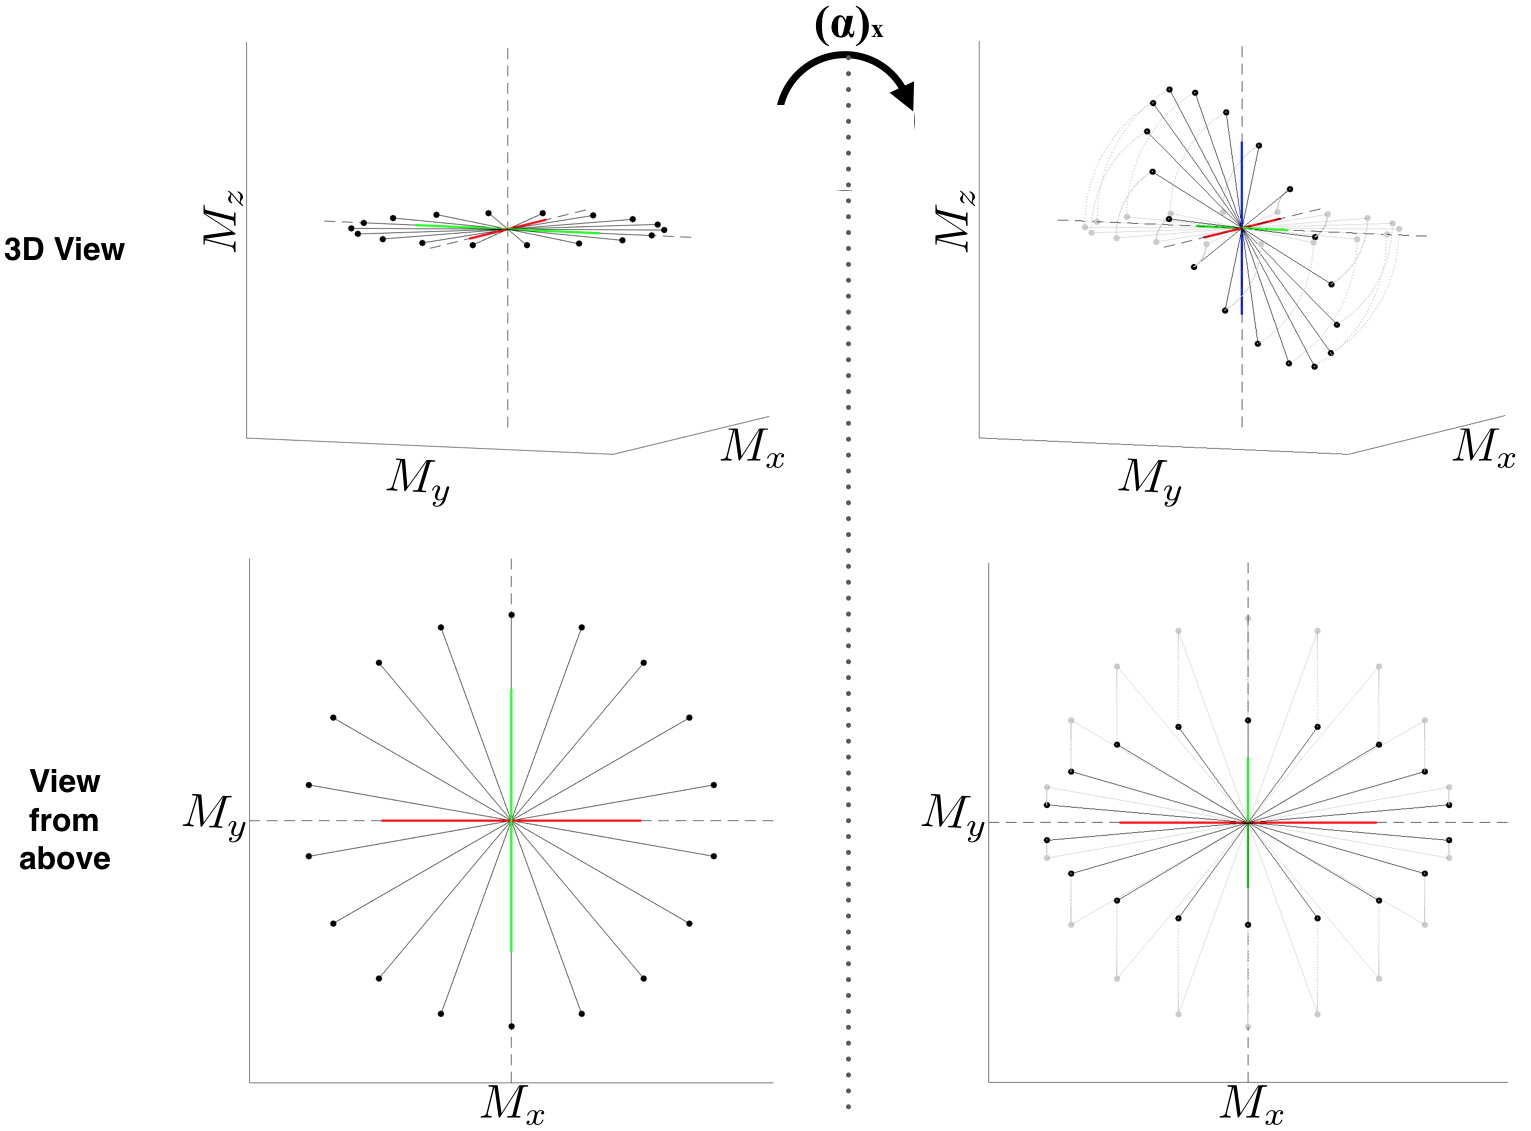
\includegraphics[angle=0,width=1\textwidth, keepaspectratio]{images/mrf/RFpulseeffect}
%     \caption{Pictorial representation of a completely dephased isochromat ensemble experiencing an ideal instantaneous $(\alpha)_x$ RF pulse.}
%     \label{fig:RFpulseeffect}
% \end{figure}
The transition to configuration states is straight forward, as the complex magnetisation vectors can be easily replaced with the partition states (the details of which are found in Hennig \cite{Hennig1991}).
Equation \ref{eq:magnbeforestates} becomes:

\begin{equation}\label{eq:magnafterstates}
    \begin{bmatrix} 
    F_{k} \\
    F_{-k} \\
    Z_{k}
    \end{bmatrix}^+ = 
        T_{\phi}(\alpha)
    \begin{bmatrix} 
    F_{k} \\
    F_{-k} \\
    Z_{k}
    \end{bmatrix}^-
\end{equation}

\hfill 

Expanding equation \ref{eq:magnafterstates} into its components yields:
\begin{equation}\label{eq:woessner}
\begin{split}
    F_{k}^+ &= F_{k}^- cos^2(\alpha/2) + e^{2i\phi} F_{-k}^- sin^2(\alpha/2)  - i e^{i \phi} Z_{k}^- sin(\alpha)  \\
    F_{-k}^+ &=  e^{-2i\phi} F_{k}^- sin^2(\alpha/2) + F_{-k}^- cos^2(\alpha/2) + i e^{-i \phi} Z_{k}^- sin(\alpha) \\
    Z_{k}^+ &= - i/2 e^{-i \phi} F_{k}^- sin(\alpha) + i/2 e^{-i \phi} F_{-k}^- sin(\alpha) + Z_{k}^- cos(\alpha) 
\end{split}
\end{equation}
which is known as the \textbf{Woessner decomposition} and it shows that in the case of an arbitrary RF pulse, the population of isochromats is redistributed among states with the same amount of dephasing $k$ \cite{Hennig1991}.

\begin{figure}[H]
    \centering
    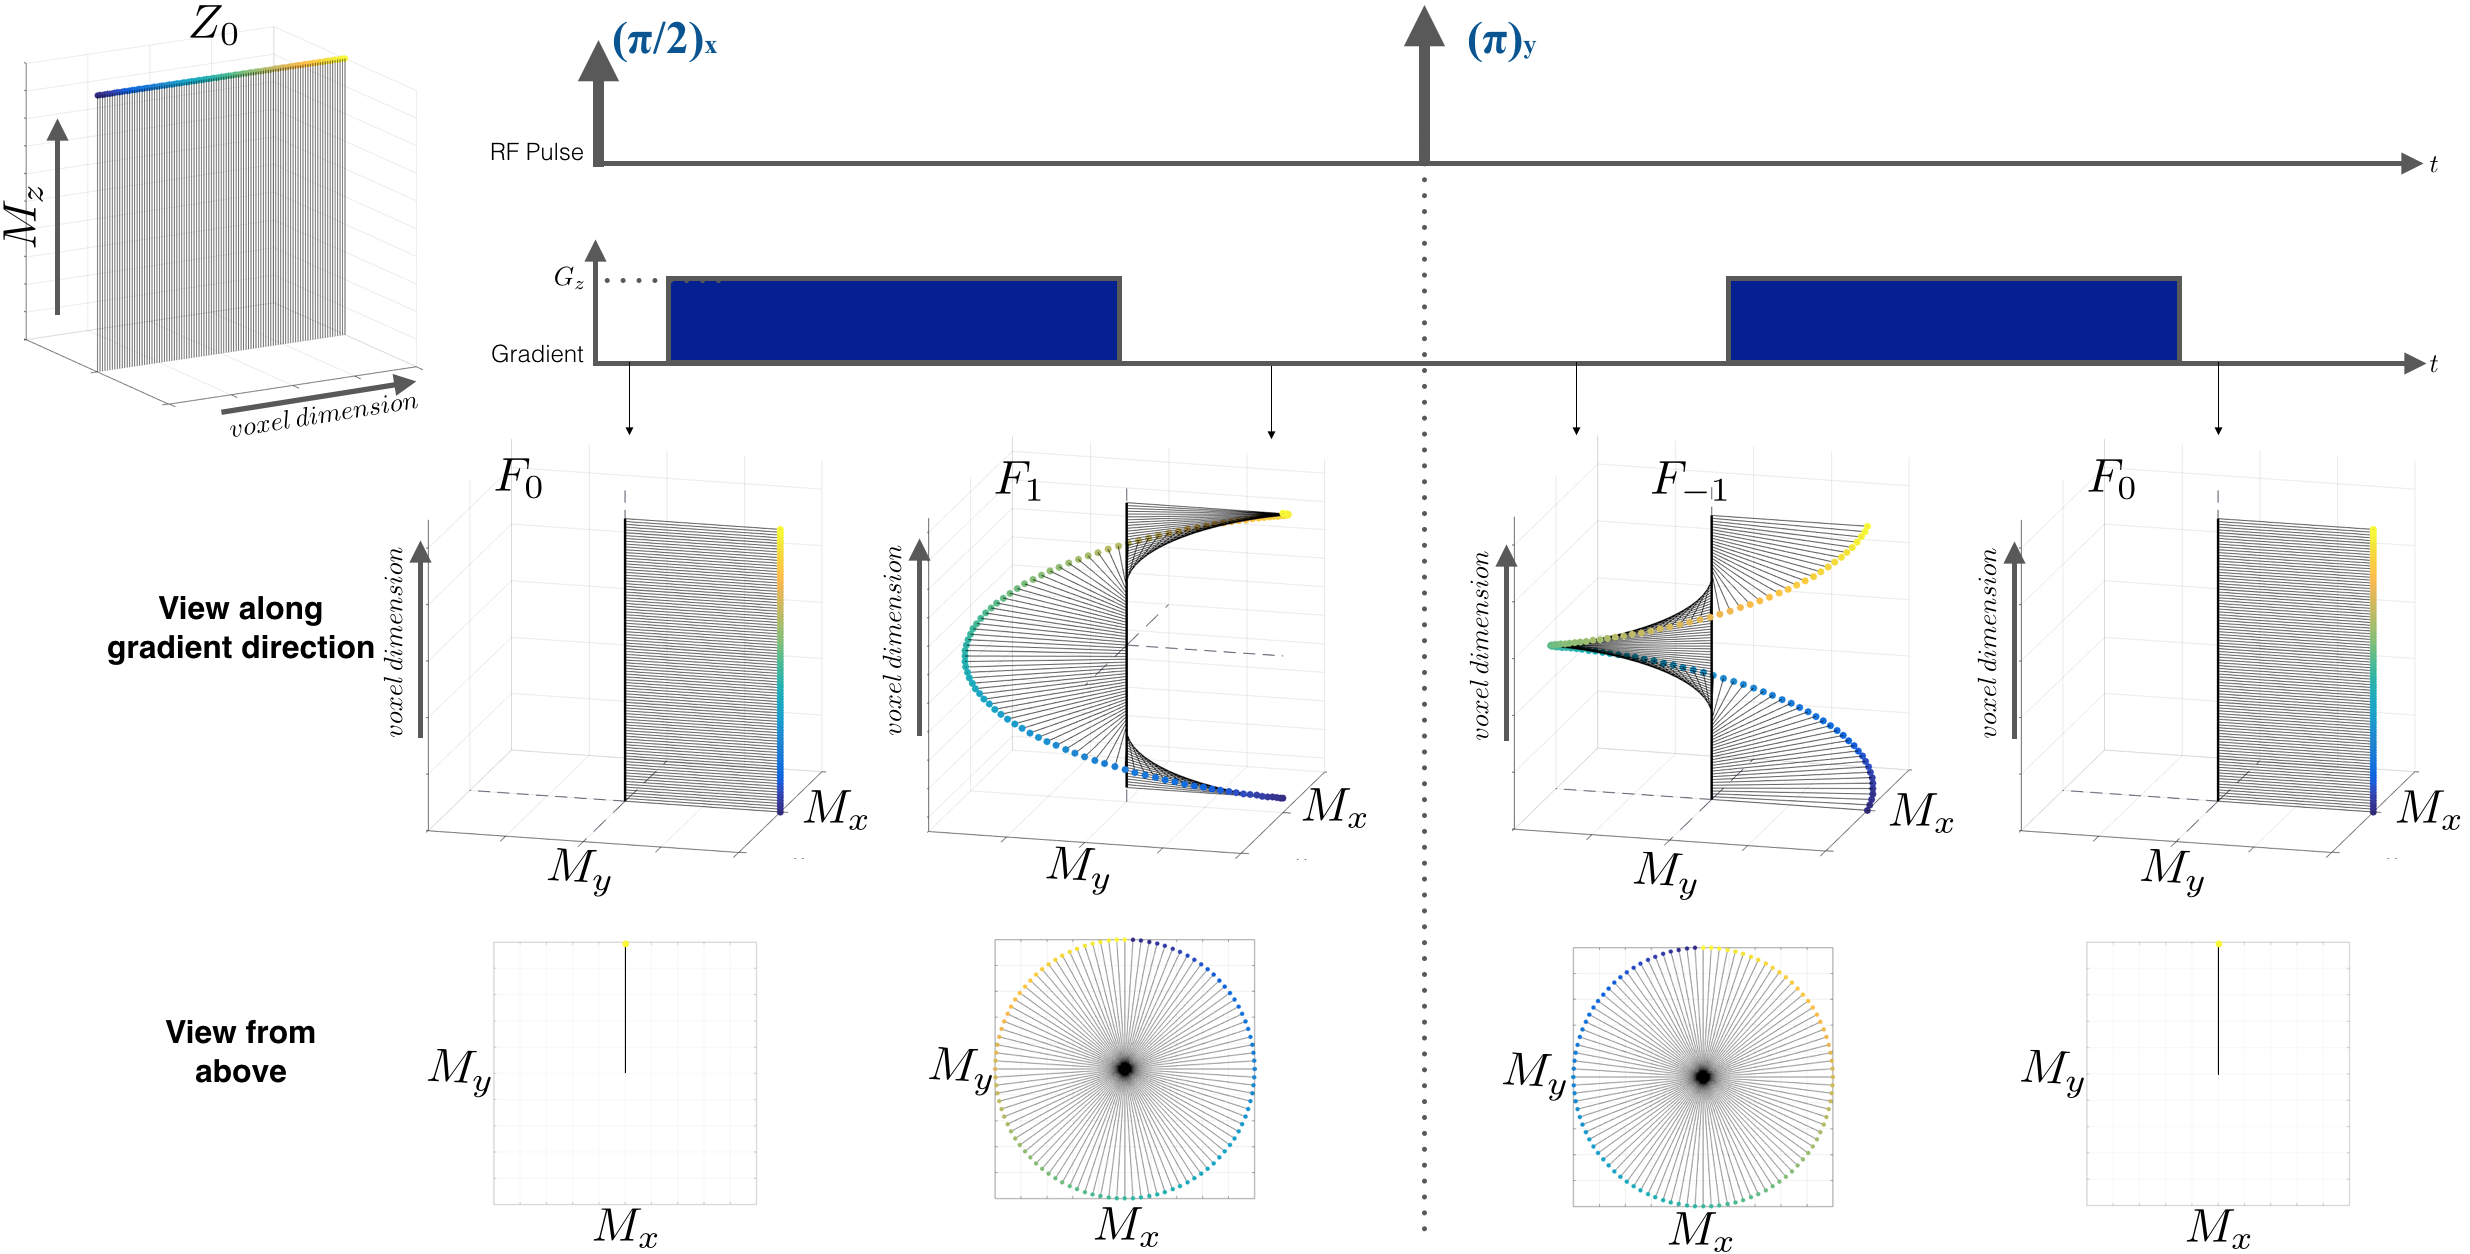
\includegraphics[angle=90,width=0.6\textwidth, keepaspectratio]{images/mrf/spinechoinepg}
    \caption{Pictorial representation of the formation of a spin echo.
    The first RF pulse flips the distribution of isochromats into the $\bm{F_0}$ configuration.
    The application of the gradient dephases the spins until the $\bm{F_1}$ configuration is formed.
    The application of the second RF pulse of flip angle $180^o$ yields the $\bm{F_{-1}}$ configuration.
    The application of the second gradient rephases the spins until they reach the coherent state $\bm{F_0}$ and an echo is formed.}
    \label{fig:spinechoinepg}
\end{figure}

The formation of the $F_{-k}$ states is best explained through an example where an RF pulse of $\alpha = \pi$ and $\phi = \pi/2$ (rotation about the y-axis) is applied on an $\bm{F_1}$ configuration.
Introducing these values in equation \ref{eq:woessner} yields:

\begin{equation}
\begin{split}
    F_{1}^+  &= - F_{-1}^- = 0 \\
    F_{-1}^+ &= - F_{1}^-  \\
    Z_{1}^+  &= - Z_{1}^- = 0
\end{split}
\end{equation}
where the $F_{-1}^-$ and $Z_{1}^-$ were set to $0$ because they were non-existent prior to the RF pulse application.
This shows that the $F_{-1}$ configuration is now formed as a consequence of applying an $180^o$ refocusing pulse.
This is the mechanism through which spin echoes are formed and a pictorial example of this happening is shown in Figure~\ref{fig:spinechoinepg}.

\hfill

The formation of the $Z_{k}$ states is best explained through an example where the RF pulse has a flip angle $\neq \pi$.
Let there be an RF pulse of flip angle $\alpha = \pi/4$ and phase angle $\phi = 0$ applied on an $\bm{F_1}$ configuration.
Introducing these values in equation \ref{eq:woessner} yields:

\begin{equation}
\begin{split}
    F_{1}^+  &= F_{1}^- cos^2(\alpha/2) \approx 0.853 F_{1}^- \\
    F_{-1}^+ &= F_{1}^- sin^2(\alpha/2) \approx 0.147 F_{1}^-   \\
    Z_{1}^+  &= - i/2 F_{1}^- sin(\alpha)  \approx - 0.353 \, i \, F_{1}^-
\end{split}
\end{equation}
which shows that the application of the RF pulse lead to a partitioning of the isochromat ensemble into three configuration states: $\bm{F_1}$, $\bm{F_{-1}}$ and $\bm{Z_1}$ of different coefficients.
Figure~\ref{fig:RFPulseinEPG} shows a pictorial representation of the effect of applying the $(\pi/4)_x$ RF pulse on a dephased $\bm{F_1}$ configuration.

\begin{figure}[ht]
    \centering
    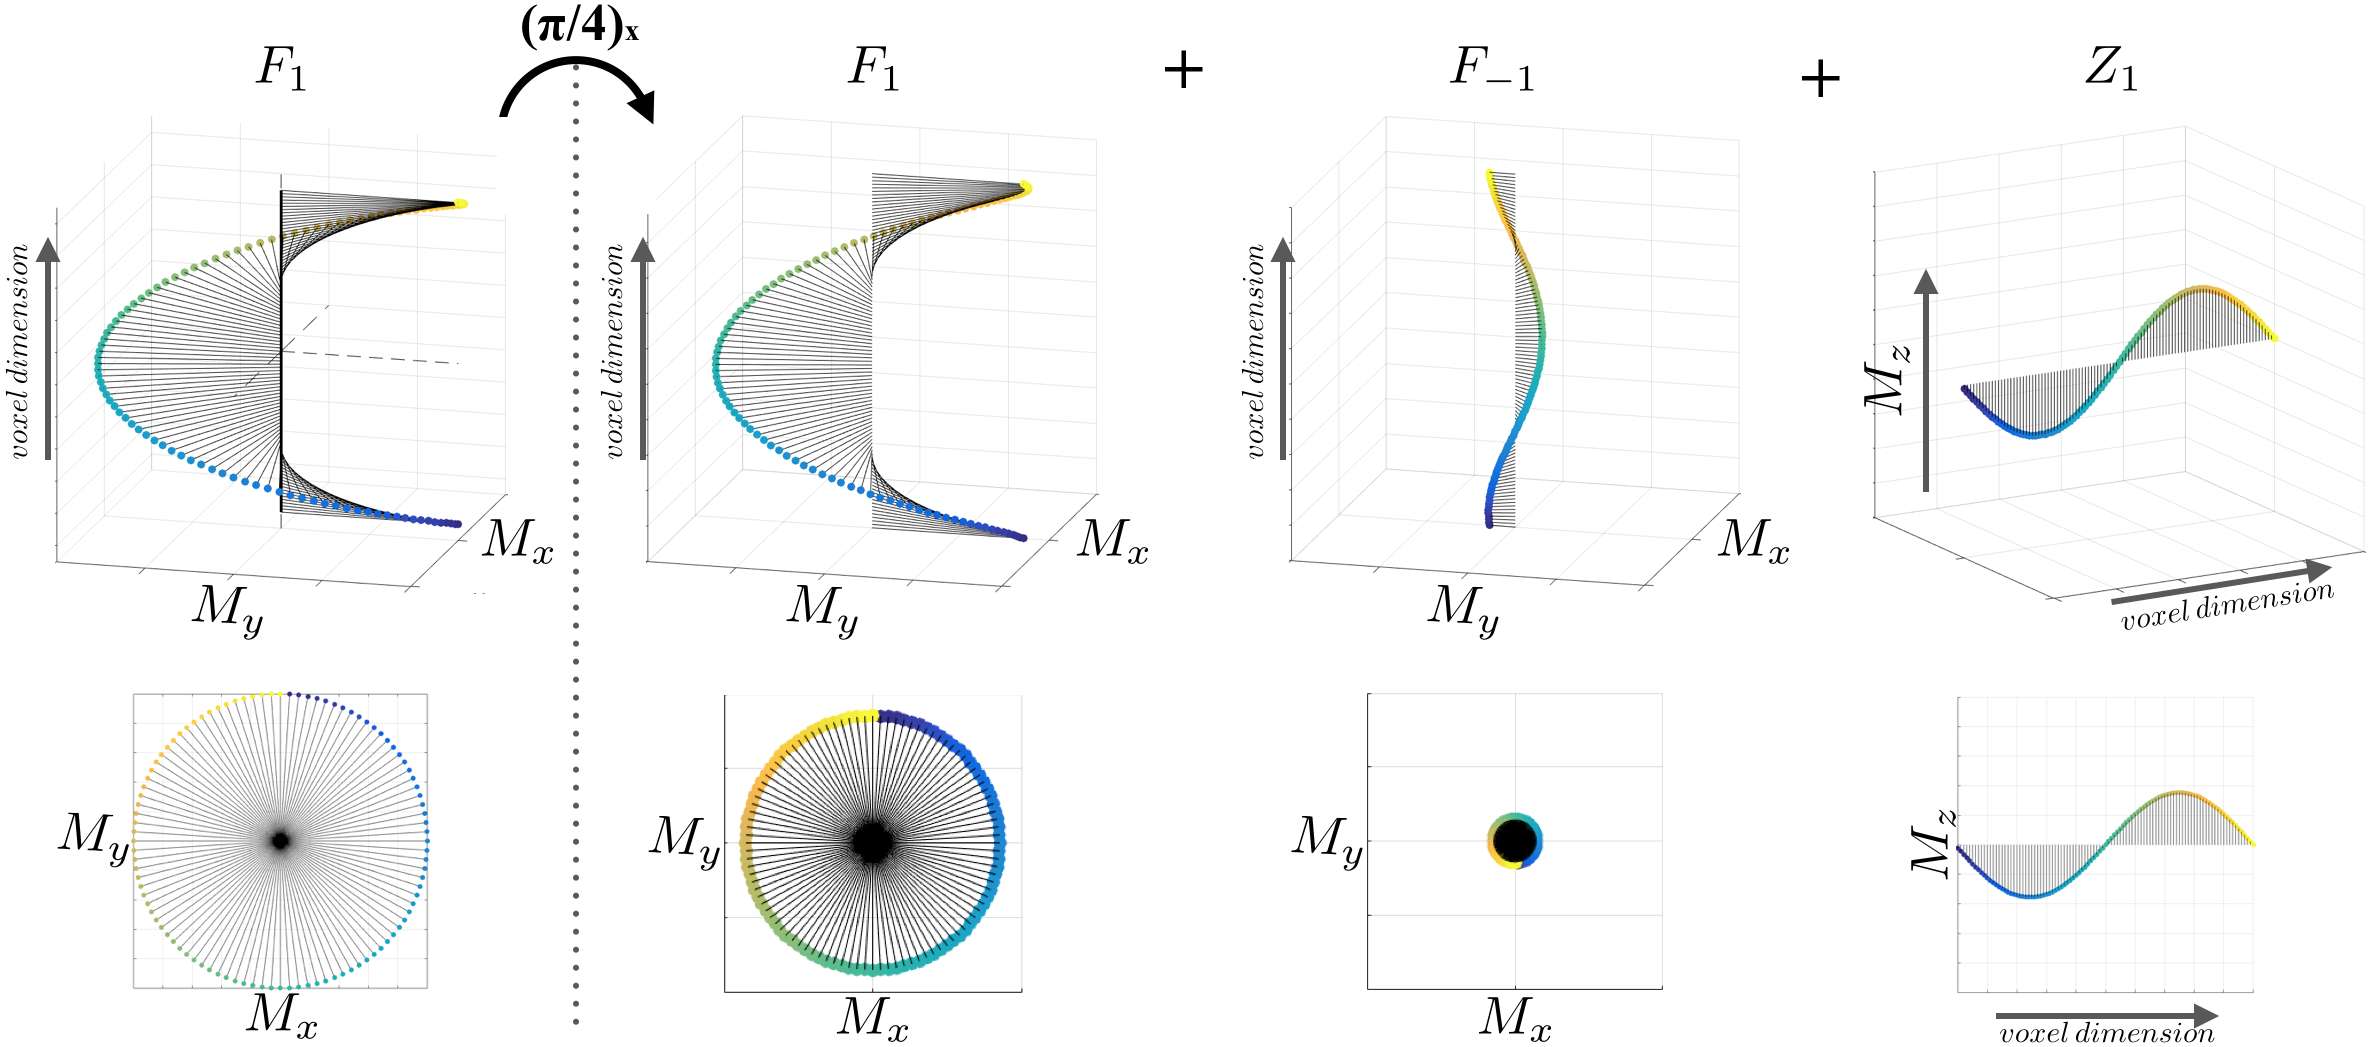
\includegraphics[angle=0,width=1\textwidth, keepaspectratio]{images/mrf/RFPulseinEPG}
    \caption{Pictorial representation of the formation of configuration states as a result of applying an RF pulse on a fully dephased $\bm{F_1}$ state.
    In this example we are showing the effect of an instantaneous RF pulse of flip angle $\alpha = \pi/4$ and phase angle $\phi = 0$ which `mixes' the populations into configuration states of the same 
    }
    \label{fig:RFPulseinEPG}
\end{figure}

\hfill

% % % % % % % % % % % % % % % % % % % % 
\textbf{Relaxation effects} 

The effects of relaxation towards thermal equilibrium can also be described in the \ac{epg} framework.
For the transverse states $T_2$ relaxation occurs: $F_k' = E_2 F_k$, while for the longitudinal states $T_1$ relaxation occurs: $Z_k' = E_1 Z_k$ (for $k \neq 0$)
%, $Z_k$ states are attenuated) 
and $Z_k' = E_1 Z_k + M_0(1 - E_1)$ (for $k = 0$).
%, $Z_k$ states experience recovery).
Here, $E_1 = e^{-\tau/T_1}$ and $E_2 = e^{-\tau/T_2}$ for a given time $\tau$.
In matrix form, this becomes \cite{Hennig1991}:

\begin{equation}\label{eq:woessnerFn}
    \begin{bmatrix}
        F_k      \\
        F_{-k} \\
        Z_k
    \end{bmatrix}' = 
    \underbrace{
    \underbrace{\begin{bmatrix}
        E_2 & 0 & 0 \\
        0 & E_2 & 0 \\
        0 & 0 & E_1 
    \end{bmatrix}
    \begin{bmatrix}
        F_k      \\
        F_{-k} \\
        Z_k
    \end{bmatrix}}_\text{for k $\neq$ 0}
    +
    \begin{bmatrix}
        0 \\
        0 \\
        M_0 (1 - E_1)
    \end{bmatrix}}_\text{for k = 0}
\end{equation}

\hfill

\large \textbf{Extended Phase Graph Algorithms} \normalsize

The \ac{epg} algorithm consists of a set of rules to be applied in order to simulate signals coming from a wide variety of MR sequences.
I start by describing the key data structures involved in the algorithm and then move on to explaining how RF pulses, dephasing gradients and relaxation phenomena are introduced in this framework.

\hfill

\textbf{EPG Data Structures}

In the \ac{epg} algorithm the set of all possible confugration states at any given time point is stored in a matrix called the `state matrix':
\begin{equation}
    \Omega = 
    \begin{bmatrix}
    F_0 & F_1 & F_2 & \dots \\
    F_0^* & F_{-1} & F_{-2} & \dots \\
    Z_0 & Z_1 & Z_2 & \dots 
    \end{bmatrix}
\end{equation}
where $\bm{F_0}$ occurs twice for completion.

\hfill

This matrix contains the three possible basis states $\bm{F_k}$, $\bm{F_{-k}}$ and $\bm{Z_k}$ in increasing dephasing order $\bm{k}$.
Although this matrix can be considered infinite in one dimension as there are infinitely many configurations, all MR experiments are finite thus limiting the matrix size to reasonable dimensions.
In fact, for the sequence I am modelling, where both the repetition time and the amount of dephasing in each period is constant, the number of branches is equal to the number of RF pulses.
Thus, the state matrix $\Omega$ is a $3 \times N_{pulses}$ complex matrix that stores the coefficients for each basis set.

\hfill

In order to store all the possible configuration states for all time points $t$ in the multi-pulse sequence, two other matrices are used, called the `evolution matrices':

\begin{equation}
    \Xi_F = 
    \begin{bmatrix}
    \vdots & \vdots & \vdots & \vdots & \dots \\
    F_2(t_0) & F_2(t_1) & F_2(t_2) & F_2(t_3) & \dots \\
    F_1(t_0) & F_1(t_1) & F_1(t_2) & F_1(t_3) & \dots \\
    F_0(t_0) & F_0(t_1) & F_0(t_2) & F_0(t_3) & \dots \\
    F_{-1}(t_0) & F_{-1}(t_1) & F_{-1}(t_2) & F_{-1}(t_3) & \dots \\
    F_{-2}(t_0) & F_{-2}(t_1) & F_{-2}(t_2) & F_{-2}(t_3) & \dots \\
    \vdots & \vdots & \vdots & \vdots & \dots 
    \end{bmatrix}
\end{equation}

and

\begin{equation}
    \Xi_Z = 
    \begin{bmatrix}
    \vdots & \vdots & \vdots & \vdots & \dots \\
    Z_2(t_0) & Z_2(t_1) & Z_2(t_2) & Z_2(t_3) & \dots \\
    Z_1(t_0) & Z_1(t_1) & Z_1(t_2) & Z_1(t_3) & \dots \\
    Z_0(t_0) & Z_0(t_1) & Z_0(t_2) & Z_0(t_3) & \dots 
    \end{bmatrix}
\end{equation}

\hfill

The evolution matrices store the state matrices, as columns, for each time point of interest.
These matrices can, again, be of infinite size, as there are infinite configurations and the time domain can be infinitely sampled.
However, for my application where both the repetition time and the amount of dephasing in each period is constant, the $\Xi_F$ evolution matrix is a $2N_{pulses}-1 \times N_{pulses}$ complex valued matrix, while the $\Xi_Z$ evolution matrix is an $N_{pulses} \times N_{pulses}$ complex valued matrix.
This is because I am only interested in the values of the coefficients at echo time in each $T_R$ block.

\hfill

\textbf{Applying an RF pulse}

RF pulses are modelled as instantaneous by applying the $T_{\phi}(\alpha)$ operator (see equation \ref{eq:woessnerFn2}) on the pre-RF pulse state matrix.
For example, for an RF pulse of flip angle $\alpha = \pi/2$ and phase angle $\phi = 0$ applied on the initial $\Omega (t < 0) = [0, 0, 1]^T$, we write:
\begin{equation}
    \Omega (t = 0) = T_0(\pi/2) \Omega (t < 0) = 
    \begin{bmatrix} 
        1 \\
        1 \\
        0
    \end{bmatrix}
\end{equation}

\hfill

\textbf{Dephasing due to gradient}

As stated before, dephasing causes a shift of configuration states.
Thus, it can be represented by a shift operator, $S$, which performs $F_k \rightarrow F_{k+1}$ and leaves the longitudinal state unchanged $Z_k \rightarrow Z_k$. 
For example, if after the application of the $\pi/2$ RF pulse a gradient is applied until the end of the repetition period, the state matrix becomes:
\begin{equation}
    \Omega (t = T_R) = S \, \, \Omega (t = 0) = 
    \begin{bmatrix} 
        0 & 1\\
        0 & 0\\
        0 & 0
    \end{bmatrix}
\end{equation}
where $S$ is the shift operator which performs $F_n \rightarrow F_{n+1}$ and leaves the longitudinal state unchanged $Z_n \rightarrow Z_n$. 
Note that the state matrix contains all possible states, which means that for this example $F_{-1} = 0$ was shifted to $F_0^*$.

\hfill

\textbf{Relaxation}

Relaxation phenomena is treated as explained previously (see equation \ref{eq:woessnerFn}):
all transverse states in the state matrix experience $T_2$ decay, all longitudinal states with $k \neq 0$ in the state matrix experience $T_1$ relaxation and longitudinal states with $k = 0$ also experience $T_1$ recovery.

\hfill

\large \textbf{Dictionary} \normalsize

In order to create a dictionary of signals for a multi-pulse \ac{fisp} sequence, the \ac{epg} algorithm was used.
As with the \ac{bssfp} case, a signal of N time points is created for each `tissue tuple'
$(T_{1_j}, T_{2_j})$, with $j \in [1, M]$, where $M$ is the total number of tuples.
For the \ac{fisp} dictionary, off-resonance frequencies were not included.
The sequence used is found in Figure~\ref{fig:sequenceFISP}, where the echo times were kept constant for every repetition block, and the unbalanced gradients achieved the same amount of dephasing in each $T_R$ block.

\hfill

To generate the signal for a given tissue type, the multi-pulse MRF-\ac{fisp} sequence was divided into $N+1$ blocks (including the inversion pulse), each of which corresponding to the application of a different RF pulse.
The signal corresponds to the $F_0$ states at echo time for each $T_R$ block.
This process was then repeated for every tissue tuple and a dictionary of $M \times N$ complex values was created.
Pseudocode for the algorithm can be found in Appendix~\ref{appendixlabel2}.

\hfill

% Prior to the second RF pulse, due to the presence of the idealised dephasing gradient,
% the spins will accrue different phases, ranging from $-\pi$ in one corner of the voxel, to $+\pi$ in the opposite corner.
% This state in which the transverse magnetisation is now found is called $F_1$ \cite{Hennig1988} \cite{Scheffler1999} and can be conceptually described as an evenly distributed collection of magnetisation vectors over the transverse plane (see Figure~\ref{fig:F1state}). 

% For a single-voxel multi-pulse \ac{fisp} experiment let us now consider that the gradient's moment induces the same amount of dephasing across this voxel during a fixed time period $\Delta t$ at the end of each repetition period.
% For an idealised gradient and an idealised voxel with uniform density of magnetisation,
% the amount of dephasing is defined by the interval $[-\pi, \pi]$.

% \hfill

% \begin{figure}[ht]
%     \centering
%     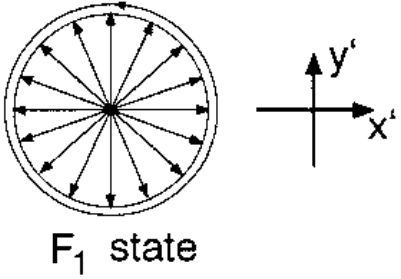
\includegraphics[angle=0,width=0.4\textwidth, keepaspectratio]{images/mrf/F1state}
%     \caption{The $F_1$ state is a magnetisation substate which describes a uniform distribution of magnetisation vectors over the transverse plane, with phases ranging from $-\pi$ to $+\pi$. Figure adapted from \cite{Scheffler1999}.}
%     \label{fig:F1state}
% \end{figure}

% \hfill

% The EPG algorithm \cite{Hennig1988} \cite{Hennig1991} \cite{Weigel2015} is a tool used to simulate signals obtained from a wide variety of MRI pulse sequences \cite{Malik2017}.
% % EPG has been used for a variety of applications such as:
% % characterization of RF spoiling in gradient echo sequences (4,5), 
% % analysis of echo amplitudes in turbo spin echo (TSE) sequences (6–9), 
% % diffusion effects (12), and 
% % characterizing signal evolution in sequences used for relaxometry (13–16).
% Similar to the Bloch equations approach, EPG characterizes a given sequence through the effects of RF pulses, relaxation constants, and dephasing due to gradients or inhomogeneities in the main magnetic field.
% % However, unlike the previous approach, EPG describes a spin system as a discrete set of phase states (or, `configuration states') \cite{Hennig1988}.
% % These states appear as a consequence of 
% To model the behaviour of a spin ensemble with known relaxation times and proton density values in a single-voxel MRF-\ac{fisp} sequence, the following assumptions were made:



% \textbf{Extended Phase Graph Formalism} 

% In the following section three key concepts that form the basis for understanding EPG are presented.
% Next, these concepts are brought together to form the EPG framework.

% \hfill

% % To understand how EPG works, we will first define the total magnetisation $M$ at thermal equilibrium as a normalised column vector $B = [0 \, 0 \, 1]^T$.
% % $B$ contains the coefficients for the $M_x$, $M_y$ and $M_z$ components of the total magnetisation M.
% % At any time point during a multi-pulse experiment, one can calculate the total magnetisation by summing over a collection of spins which are described by their corresponding x,y,z components.
% % However, to be accurate, this requires a large spin ensemble.

% % \hfill

% % In the EPG formalism the matrix $B$ is expanded to describe \textit{substates}.
% % These substates are defined as collection of spins with different $M_x$, $M_y$ and $M_z$ components and are characterised by the net magnetisation of the substate, and the space-dependent phase of the transverse magnetisation of the spin ensemble \cite{Hennig1988}.
% % In this framework, the signal intensity at any given time point during the sequence can be calculated by knowing the partitioning of the total magnetisation between the substates, and the net magnetisation in each substate.

% % \hfill

% \textbf{The effect of gradients on a spin ensemble} 

% For a single-voxel multi-pulse \ac{fisp} experiment let us now consider that the gradient's moment induces the same amount of dephasing across this voxel during a fixed time period $\Delta t$ at the end of each repetition period.
% For an idealised gradient and an idealised voxel with uniform density of magnetisation,
% the amount of dephasing is defined by the interval $[-\pi, \pi]$.

% \hfill 

% Let us consider that the first RF pulse is an ideal $90^o$ excitation pulse which flips the total magnetisation in the transverse plane.
% Prior to the second RF pulse, due to the presence of the idealised dephasing gradient,
% the spins will accrue different phases, ranging from $-\pi$ in one corner of the voxel, to $+\pi$ in the opposite corner.
% This state in which the transverse magnetisation is now found is called $F_1$ \cite{Hennig1988} \cite{Scheffler1999} and can be conceptually described as an evenly distributed collection of magnetisation vectors over the transverse plane (see Figure~\ref{fig:F1state}). 

% \begin{figure}[ht]
%     \centering
%     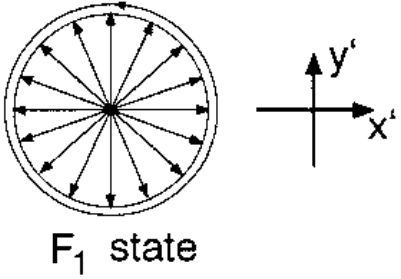
\includegraphics[angle=0,width=0.4\textwidth, keepaspectratio]{images/mrf/F1state}
%     \caption{The $F_1$ state is a magnetisation substate which describes a uniform distribution of magnetisation vectors over the transverse plane, with phases ranging from $-\pi$ to $+\pi$. Figure adapted from \cite{Scheffler1999}.}
%     \label{fig:F1state}
% \end{figure}

% \hfill

% The application of a second RF pulse will interfere with this state.
% For an arbitrary flip angle $\alpha$ and phase angle $\phi = 0$, the $F_1$ `disk' will be rotated around the RF pulse's axis of rotation.
% The newly formed transverse magnetisation can be described as two dephased states: $F^+_1$ and $F^+_{-1}$, while the longitudinal magnetisation is now known as $Z^+_1$.
% The superscript `+' denotes `immediately after the RF pulse'.
% In the EPG formalism, other states exist and they are denoted as $F_n$, depending on the amount of dephasing experienced.
% This can be seen in Figure~\ref{fig:EPGeffectofgrad}, where the $2^{nd}$ gradient pulse further dephased the $F_1$ state.
% Due to being an idealised gradient and an idealised voxel with uniform density of magnetisation, the amount of dephasing is again defined by the interval $[-\pi, \pi]$.
% This causes the spins to have now accrued phases ranging from $-2 \pi$ to $+2 \pi$.
% The presence of the gradient will therefore `transform' the $F_1^+$ state into a new state we call $F_2$.
% On the other hand, $Z^+_1$ was formed because the RF pulse `flipped' the transverse components of some of the pre-RF pulse magnetisation vectors into the longitudinal plane.
% The formation of the $F_1^+$, $F_{-1}^+$ and $Z_1^+$ states is better understood through the Woessner decomposition \cite{Woessner1961}.

% \begin{figure}[ht]
%     \centering
%     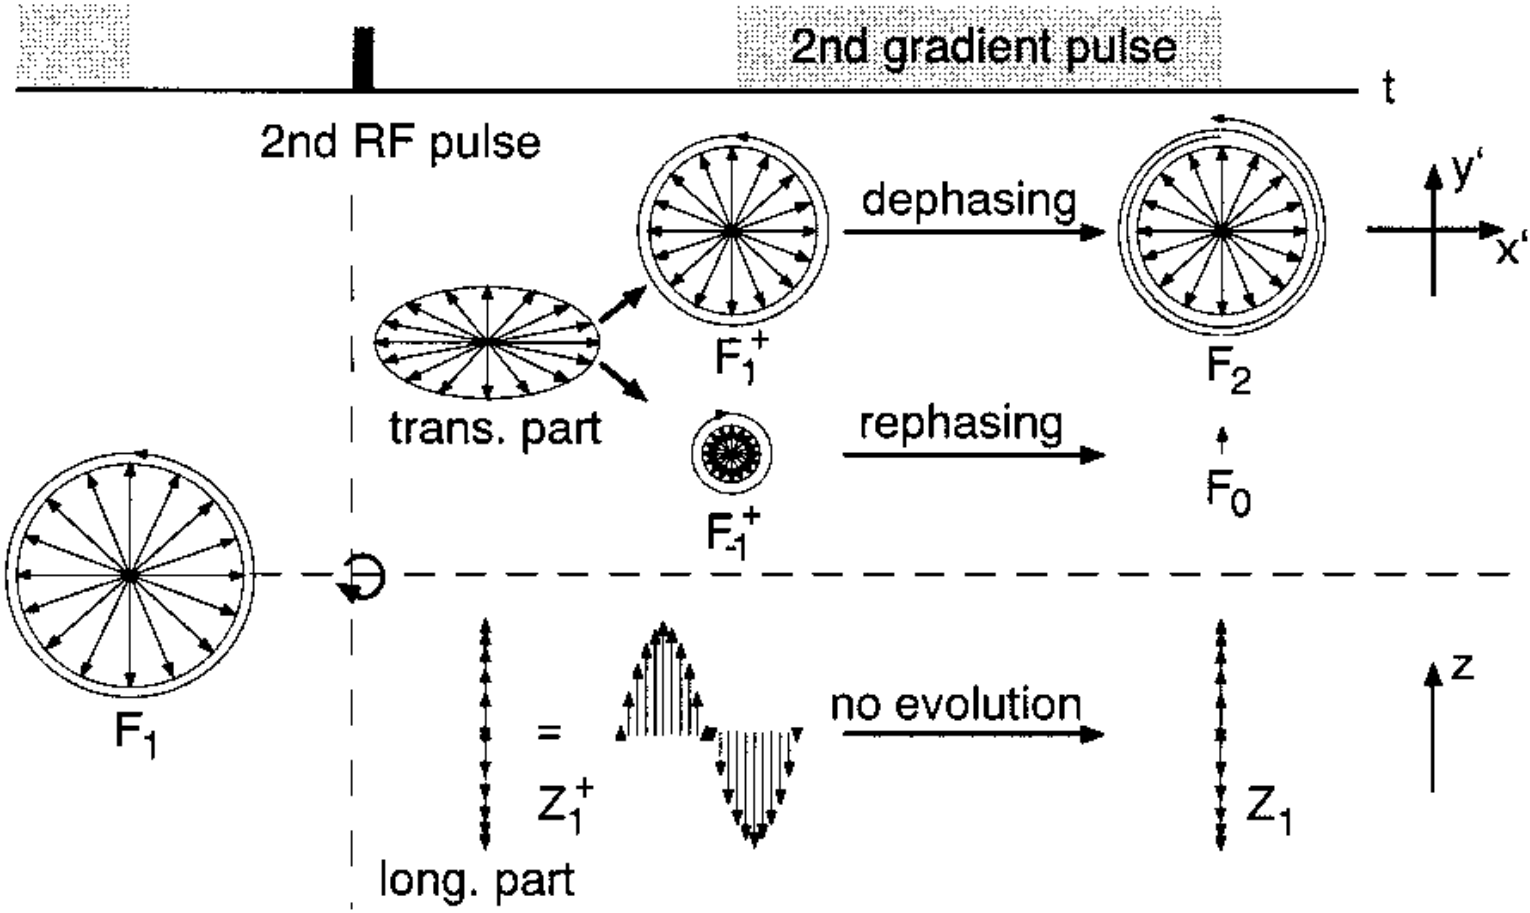
\includegraphics[angle=0,width=0.8\textwidth, keepaspectratio]{images/mrf/EPGeffectofgrad}
%     \caption{A second RF pulse will `split' the previous $F_1$ configuration into two separate transverse state configurations $F_1^+$ and $F_{-1}^+$, and a longitudinal state $Z_1^+$; this process is best described with the \textit{Woessner decomposition}. During the application of the dephasing gradient, the longitudinal state remains unaffected, while the transverse states are further dephased $F_1^+ \rightarrow F_2$, and rephased $F_{-1}^+ \rightarrow F_0$, respectively. Figure adapted from \cite{Scheffler1999}.}
%     \label{fig:EPGeffectofgrad}
% \end{figure}

% \hfill

% \textbf{Woessner decomposition.} The Woessner decomposition describes the behaviour of a complex magnetisation vector $F = M_x + i M_y$ subject to an RF pulse of arbitrary flip angle $\alpha$ and phase angle $\phi$.
% As stated before, the effect of an RF pulse can be written as a rotation matrix, which, when applied to the complex magnetisation vector yields \cite{Haacke1999} \cite{Scheffler1999}:

% \begin{equation}\label{eq:woessner}
% \begin{split}
%     F^+ &= F^- cos^2(\alpha/2) + e^{2i\phi} (F^-)^* sin^2(\alpha/2)  - i e^{i \phi} M_z^- sin(\alpha)  \\
%     M_z^+ &= - i/2 e^{-i \phi} F^- sin(\alpha) + i/2 e^{-i \phi} (F^-)^* sin(\alpha) + M_z^- cos(\alpha) 
% \end{split}
% \end{equation}
% where the superscript \textbf{+} represents immediately `after the RF pulse' and the superscript \textbf{-} represents immediately `before the RF pulse'.

% \hfill

% To make the transition to fully dephased transverse states $F_n$ and longitudinal states $Z_n$, we need to take into account the fact that an $F_n$ state represents a collection of dephased spins at different spatial positions within the idealised voxel.
% For a one-dimensional voxel, the phase of a spin at position $x$ induced by n identical gradient lobes evolves with $e^{i \, n \, \, \gamma G_x x \, \Delta t }$, where $G_x$ is the amplitude of the gradient and $\Delta t$ is its duration.
% For all positions r in the voxel, the dephased transversal state can be written as a sum over all positions: $ F_n \int_r \, dr \, e^{i \, n \, \, \gamma G r \, \Delta t }$, where the amplitude of the complex number $F_n$ represents the magnitude of this state's population.
% Similarly, the longitudinal state can be described as $ Z_n \int_r \, dr \, e^{i \, n \, \, \gamma G r \, \Delta t }$.

% \hfill

% \textbf{RF Pulse. } Introducing the complex dephased states in equations \ref{eq:woessner} and transforming into matrix representation, we can write:

% \begin{equation}\label{eq:woessnerFn1}
%     \begin{bmatrix}
%         F_n      \\
%         F_{-n}^* \\
%         Z_n
%     \end{bmatrix}^+ = 
%     T_{\phi}(\alpha)
%     \begin{bmatrix}
%         F_n      \\
%         F_{-n}^* \\
%         Z_n
%     \end{bmatrix}^- 
% \end{equation}
% where
% \begin{equation}\label{eq:woessnerFn2}
%     T_{\phi}(\alpha) = 
%     \begin{bmatrix}
%         cos^2(\alpha/2) & e^{2i\phi} sin^2(\alpha/2) & - i e^{i \phi} sin(\alpha) \\
%         e^{-2i\phi} sin^2(\alpha/2) & cos^2(\alpha/2) & i e^{-i \phi} sin(\alpha) \\
%         - i/2 e^{-i \phi} sin(\alpha) & i/2 e^{i \phi} sin(\alpha) & cos \alpha
%     \end{bmatrix}
% \end{equation}

% and the $F^*_{-n}$ state represents the complex conjugate of the $F_n$ state.

% \hfill

% Equations \ref{eq:woessnerFn1} and \ref{eq:woessnerFn2} show that, given an ensemble of spins, an RF pulse with flip angle $\alpha$ and phase angle $\phi$ will redistribute the population into different states.
% For example, different amounts of the pre-RF pulse $F^-_n$ state can now be found in both the post-RF pulse transverse state $F^+_n$ and the longitudinal state $Z_n$.
% The population represented by $F^*_{-n}$ state can be interpreted as an isochromat population whose phase was instantaneously inverted by the RF pulse, and which can be rephased later.

% % % % % % % % % % % % % % % % % % % % % % % % % % % % % % % % % % % % % % % % % % % % % % % % % % % % % % % % % % % % % % % % % % % % % % % % % % % % % % % % % % % % % % % % % % % % % % % % % % % % % % % % % % % % % % % % % % % % % % % % % % % % % % % % % % % % % % % % % % % % % % % % 
\subsection{Image Space Simulation}
\label{method:imagespace}

The second step in the simulation framework consists of the image space simulation of an IR-bSSFP MRF experiment.
This involves four components (digital object, acquisition sequence, reconstruction and motion) which are covered next.

% % % % % % % % % % % % 
\subsubsection{Digital Object}

For the simulations involved a digital phantom of $80mm$ in diameter, consisting of 12 circular structures of $5mm$ in diameter was created.
The resolution of this phantom is of $1mm$.
%, and the spin density was chosen such that there is a single spin isochromat present at each spatial location $\vec{r}$ in the phantom.
The distribution of $T_1$ and $T_2$ relaxation times is shown in Figure~\ref{fig:inputObject}, while the spin density is set to $\rho(\vec{r}) = 1$ everywhere inside the phantom, except for the space between the `tubes' and the circular phantom.
The range of values chosen for the relaxation times are also summarised in Appendix~\ref{appendixlabelPhantom}.

\begin{figure}[ht]
    \centering
    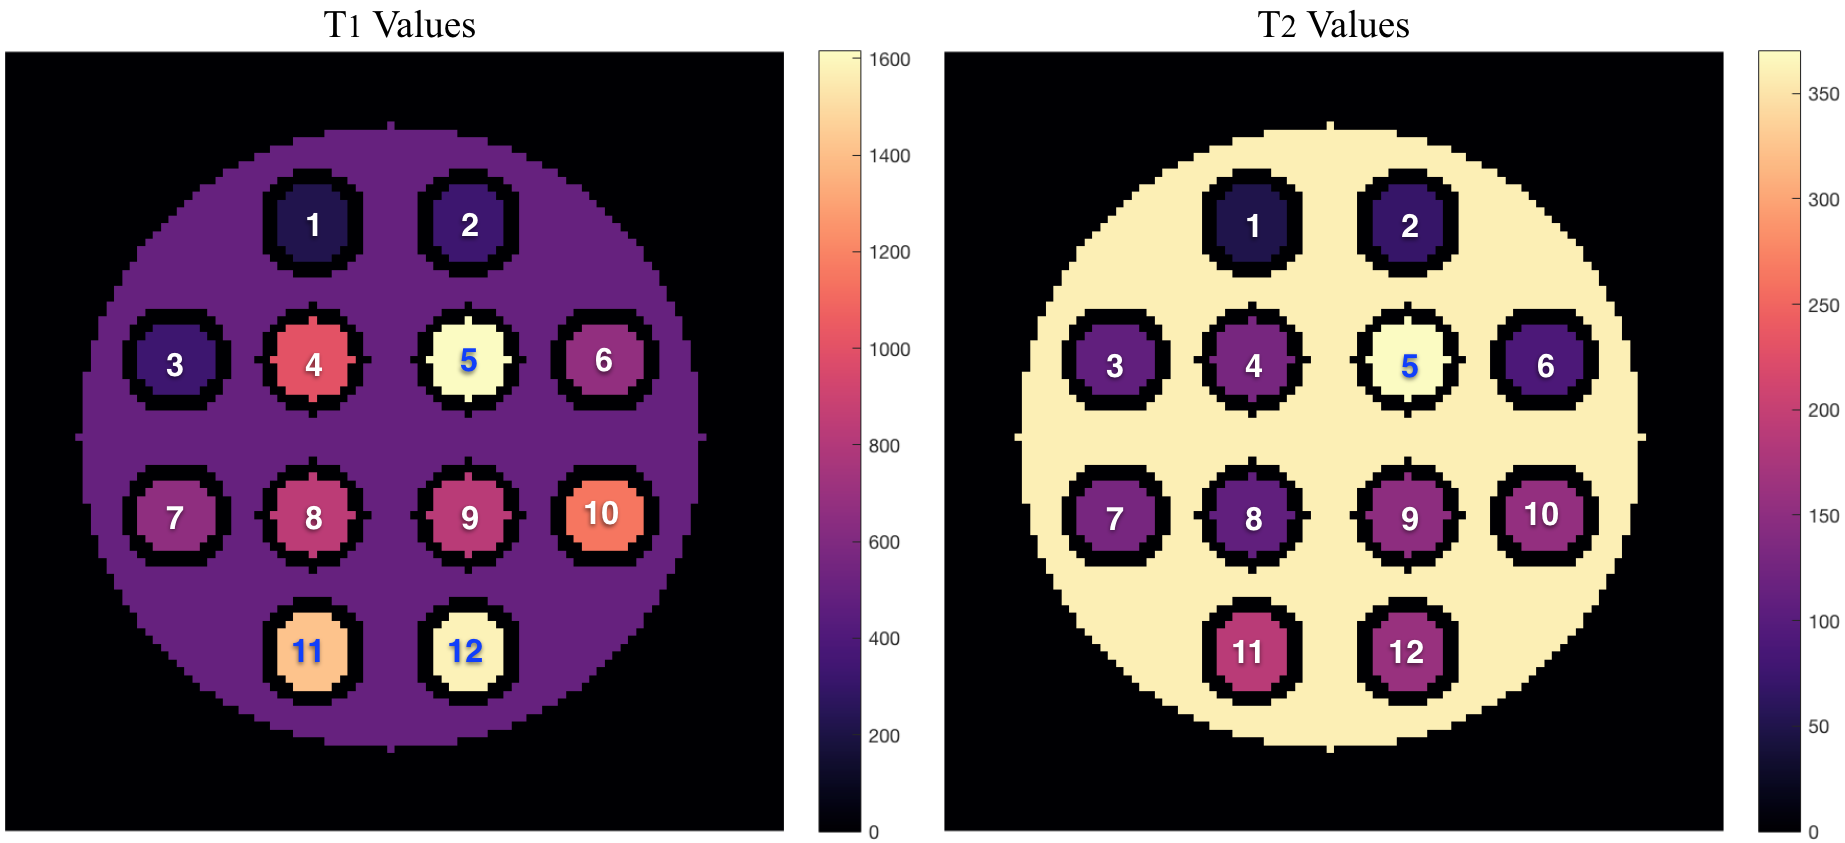
\includegraphics[angle=0,width=1\textwidth, keepaspectratio]{images/mrf/inputObject}
    \caption{The input object is a circular phantom of $80mm$ in diameter, consisting of 12 circular structures of $5mm$ in diameter. Each `tube' (shown here with indices ranging from 1 to 12) has a different $T_1$ and $T_2$ value. Similarly, the surrounding structure has its own relaxation parameters (index 0). $T_1$ and $T_2$ values are summarised in a table in Appendix~\ref{appendixlabelPhantom}.}
    \label{fig:inputObject}
\end{figure}

\hfill

The choice of digital phantom structure and composition is based on the \textit{Eurospin} 
phantom set, Test Object 5 (TO5), which contains 12 holes for agarose gel sample tubes with different relaxation properties \cite{Ihalainen2004} (see Figure~\ref{fig:realPhantom}).
The values for the relaxation times were chosen from the provided $T_1$ and $T_2$ Eurospin Appendix table and correspond to 12 of the 18 available tubes.
Moreover, this type of phantom was used in previous MRF studies such as those presented in \cite{Doneva2016} and \cite{Sommer2017}.

\begin{figure}[ht]
    \centering
    
\includegraphics[angle=0,width=0.4\textwidth, keepaspectratio]{images/mrf/realPhantom}
    \caption{The figure shows the Eurospin Test Object 5 (TO5) real phantom used for MRI quality control.
    More specifically, the TO5 of the Eurospin phantom set is used for measuring $T_1$ and $T_2$ precision and accuracy.
    The object consists of a homogeneous cylinder with 12 holes in which sample tubes of different gels with different relaxation properties can be inserted. Image courtesy of \cite{Ihalainen2004}.}
    \label{fig:realPhantom}
\end{figure}

% % % % % % % % % % % % 
\subsubsection{Acquisition}

The sequence used for the image space simulations is based on the initial implementation of the MRF framework by Ma et al. \cite{Ma2013} and is known as an inversion recovery balanced steady state free precession sequence (IR-\ac{bssfp}).
The sequence diagram is shown in Figure~\ref{fig:sequencebSSFP}.
The only difference between the sequence used for the dictionary generation part and the one used for the image acquisition part of the simulations is that the latter one was equipped with a spiral readout of duration $6 ms$.
Moreover, the spiral readout is accompanied by rewinding gradients that take the trajectory back to the centre of k-space and also assure that the zeroth moment of all gradients is zero at the end of a repetition period.

\begin{figure}[ht]
    \centering
    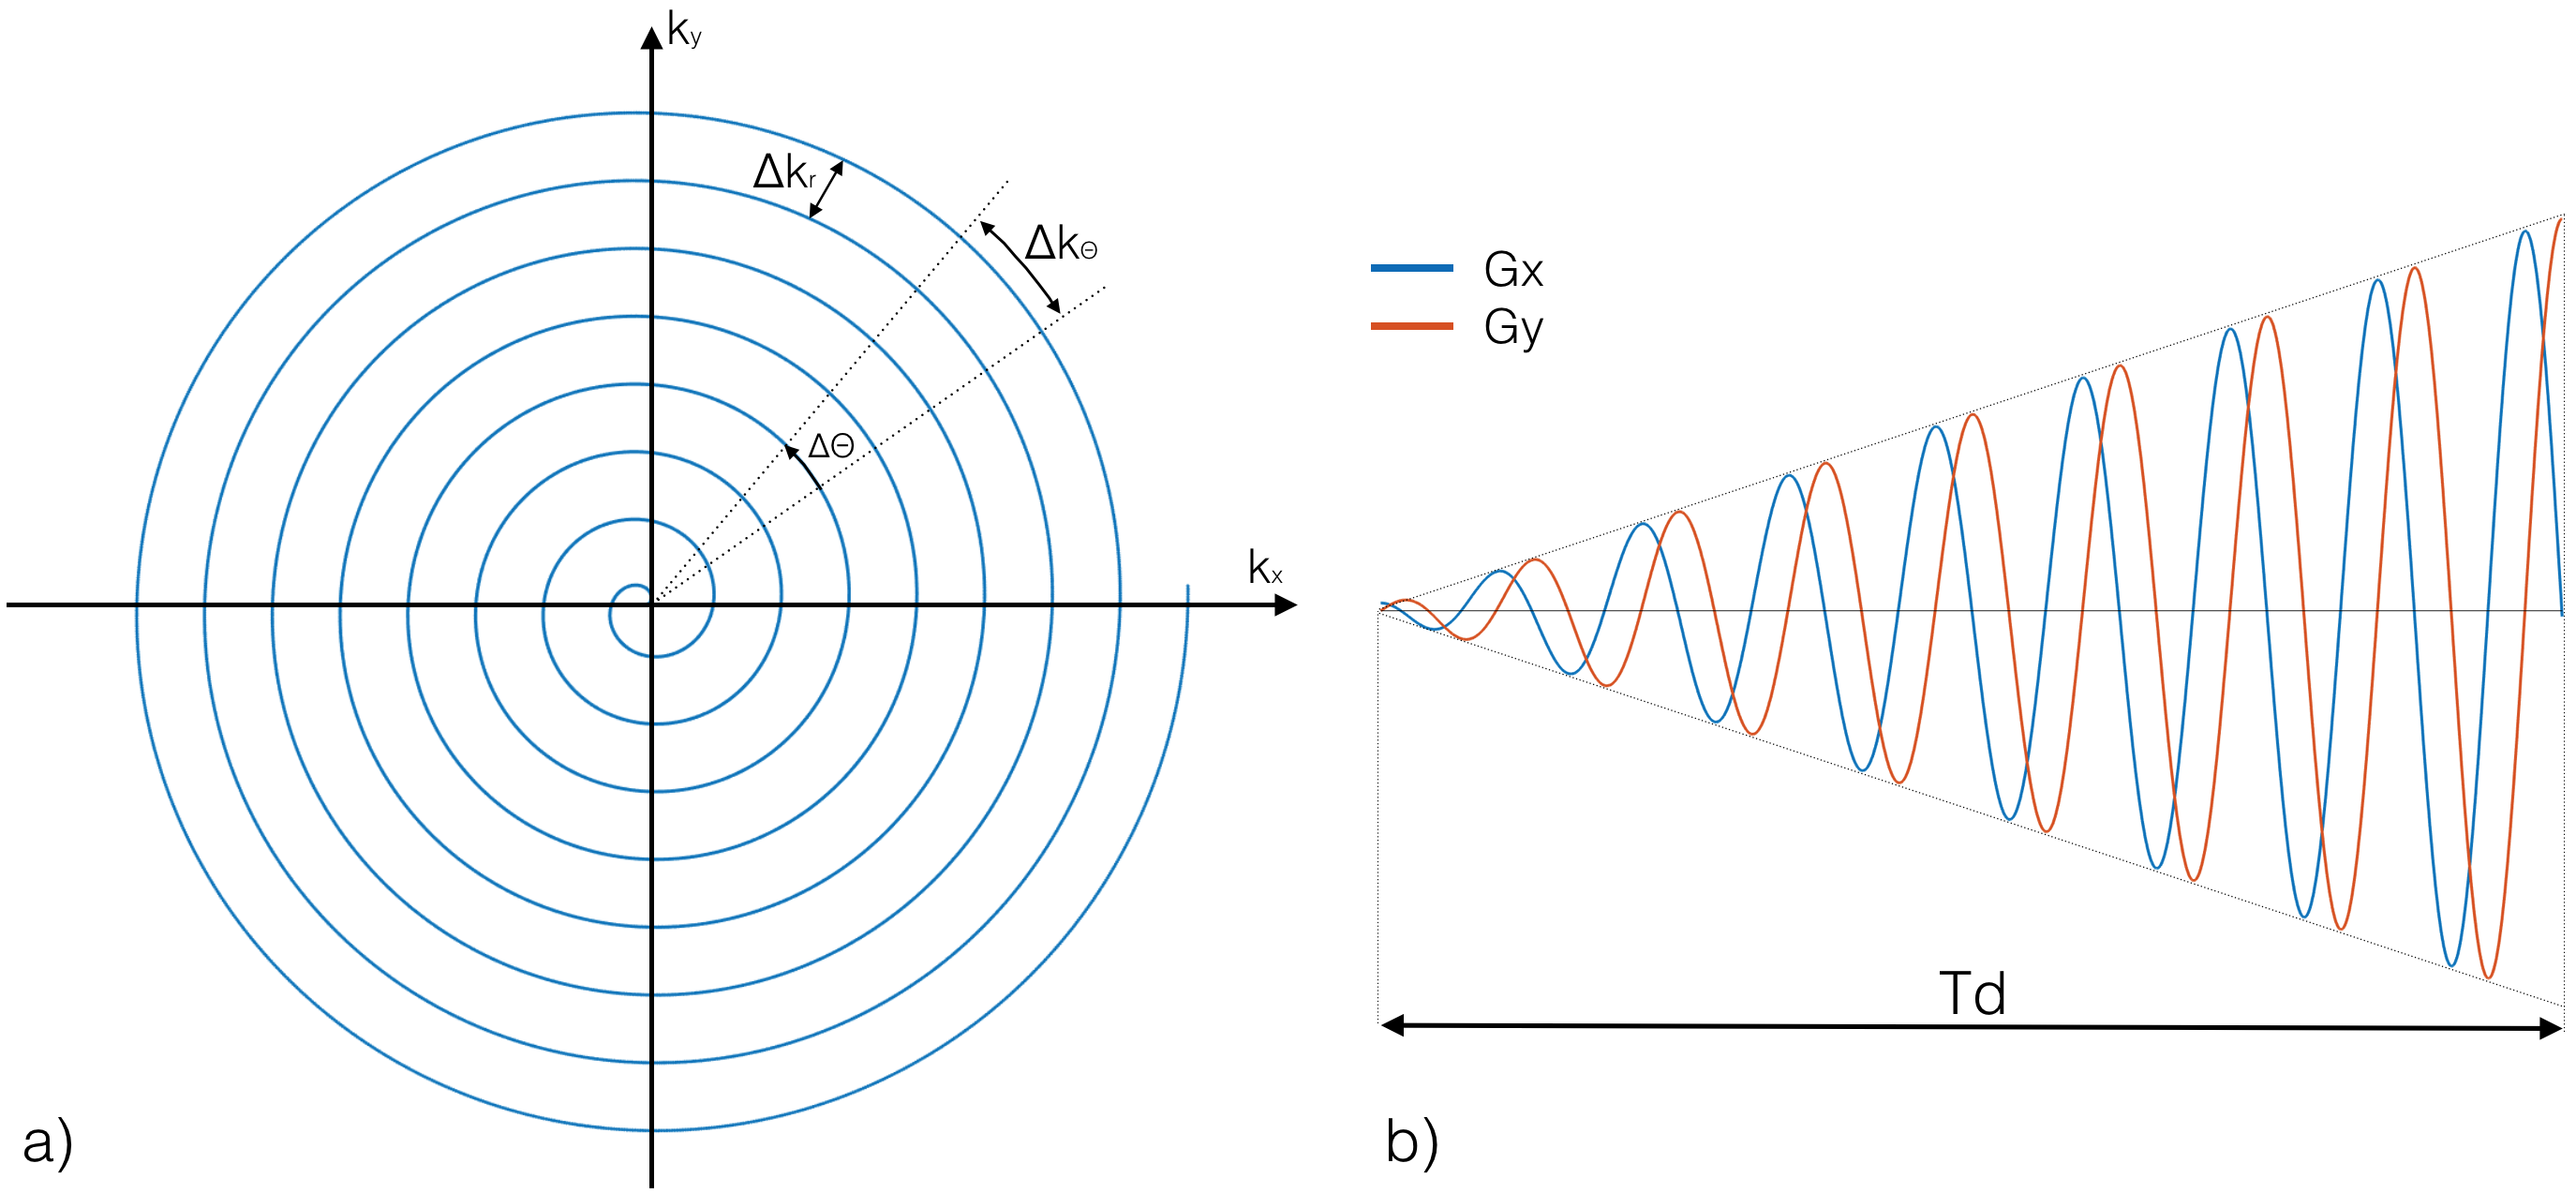
\includegraphics[angle=0,width=1\textwidth, keepaspectratio]{images/mrf/spiralAcquisition}
    \caption{An illustration of the linearly increasing spiral acquisition, showing a) the k-space trajectory and b) the corresponding gradient shape for this trajectory}
    \label{fig:spiralAcquisition}
\end{figure}

\hfill

The spiral readout was constructed in JEMRIS by analytically describing the shape of the k-space trajectory.
While different spiral coverages of k-space exist, for my simulations I chose a linearly increasing sinusoidal form, also known as a constant angular velocity (Archimedean) spiral trajectory first proposed by Ahn et al. \cite{Ahn1986}. 
Mathematically, the k-space trajectory takes the following form:

\begin{equation}\label{eq:kspacespiral}
    \begin{split}
        k_x(t) &= \text{\sout{$\gamma$}} \, \, \alpha_1 t \, \, cos (\alpha_2 t) \\
        k_y(t) &= \text{\sout{$\gamma$}}  \, \, \alpha_1 t  \, \, sin (\alpha_2 t) 
    \end{split}
\end{equation}

where $\alpha_1$ determines the gradient amplitude and $\alpha_2$ determines the angular frequency.
From equation \ref{eq:kspacespiral} and from knowing that $k_x(t) = \text{\sout{$\gamma$}} \, \, \int_0^t G_x(t') dt'$ and $k_y(t) = \text{\sout{$\gamma$}} \, \, \int_0^t G_y(t') dt'$ (see equation \ref{eq:kspace}), the desired time domain gradients can be found:

\begin{equation}
    \begin{split}
        G_x(t) &= \frac{1}{\text{\sout{$\gamma$}}} \frac{d}{dt} \,\, [k_x(t)] = \alpha_1 cos (\alpha_2 t) - \alpha_1 \alpha_2 t sin (\alpha_2 t) \\
        G_y(t) &= \frac{1}{\text{\sout{$\gamma$}}} \frac{d}{dt} \,\, [k_y(t)] = \alpha_1 sin (\alpha_2 t) + \alpha_1 \alpha_2 t cos (\alpha_2 t) 
    \end{split}
\end{equation}

The shape of both the k-space trajectory and the gradient waveforms can be seen in Figure~\ref{fig:spiralAcquisition}, where $t \in [0, T_d]ms$.

\hfill

Constant angular velocity Archimedean spirals have constant step sizes in both radial ($\Delta k_r$) and azimuthal directions ($\Delta k_{\theta}$).
The values for these step sizes can be found by considering the sampling requirements imposed by the Nyquist criterion.
For this, we first need to rewrite the k-space trajectory in polar coordinates:
\begin{equation}
    \begin{split}
        k_r(t) &= \sqrt{k_x^2(t) + k_y^2(t)} = \text{\sout{$\gamma$}} \alpha_1 t \\
        k_{\theta}(t) &= tan^{-1} \Bigg[ \frac{k_y(t)}{k_x(t)} \Bigg] = \alpha_2 t
    \end{split}
\end{equation}

Now, considering constant numbers of sampling points per winding $n_{\theta}$ and radially $n_r$, and knowing that two radial points are exactly $2\pi$ apart, both angular and radial step sizes can be defined:
\begin{equation}\label{eq:deltak1}
    \Delta k_r = \text{\sout{$\gamma$}} \alpha_1 n_{\theta} \Delta t  \, \, \text{  and  } \, \, \Delta k_{\theta} = \alpha_2 \Delta t
\end{equation}
where $\Delta t$ is the sampling rate.
% \Delta k_r = k_r(t) \rvert_{t=t'+2\pi/\alpha_2} + k_r(t) \rvert_{t=t'}
To find the required number of sampling points, we can also write:
\begin{equation}\label{eq:deltak2}
    \Delta k_r = \frac{k_{max}}{n_r} = \frac{1}{2 \Delta r n_r} \leq \frac{1}{L} \, \, \text{  and  } \, \,  \Delta k_{\theta} = k_{max} \Delta \theta = \frac{2 \pi}{2 \Delta r n_{\theta}} \leq \frac{1}{L} 
\end{equation}
where $\Delta r$ is the image resolution.
Therefore, for a fully sampled spiral we choose: $n_r \geq L / 2 \Delta r$ and $n_{\theta} \geq \pi L / \Delta r$.

\hfill

Explicit values for $\alpha_1$ and $\alpha_2$ are found from equations \ref{eq:deltak1} and \ref{eq:deltak2}:
\begin{equation}
    \alpha_1 = \frac{\pi}{\text{\sout{$\gamma$}} n_{\theta} n_r \Delta t \Delta r}  \, \, \text{  and  } \, \, \alpha_2 = \frac{2 \pi}{n_{\theta} \Delta t}
\end{equation}
%The total required acquisition time will therefore be: $T_d = n_r n_{\theta} \Delta t$.
and
\begin{equation}
    \Delta t = \frac{T_d}{n_r n_{\theta}}
\end{equation}

\hfill

To reconstruct the input object, a circular field-of-view of $160mm$ was covered with a matrix size of $128 \times 128$.
This resulted in an image resolution of $\Delta r = 1.25mm$ and required
%a square field-of-view of $160 \times 160mm$ was covered with a matrix size of $128 \times 128$.
%with an image resolution of $\Delta r = 1.25mm$,
%circular field-of-view of $160mm$ diameter encompassing our object.
%This means that our image resolution was $\Delta r = 1.25mm$.
%Therefore, we required $n_r \geq \frac{L}{2 \Delta r} = 64$ and
$n_r \geq \frac{L}{2 \Delta r} = 64$ and
$n_{\theta} \geq \frac{\pi L}{\Delta r} = 403$.
This means that in every readout there were approximately $25,792$ samples acquired.
For a total acquisition time of $T_d = 6ms$, I calculated a dwell time of $\Delta t = 0.233 \mu s$.
The slice thickness was set to $1mm$, but as I used a 2D input object, there were no slice selection gradients introduced in the simulations.

% Now, considering a constant number of sampling points per winding $n_{\theta}$ and an angular step size $\Delta \theta$, the complete angular coverage of one full turn of the spiral is defined by:
% \begin{equation}
%     2\pi = n_{\theta} \Delta \theta
% \end{equation}
% Moreover, since an angle $\Delta \theta$ is covered at each sampling interval $\Delta t$, the angular frequency $\alpha_2$ becomes:
% \begin{equation}
%     \alpha_2 \equiv \frac{\Delta \theta}{\Delta t} = \frac{2\pi}{n_{\theta}\Delta t}
% \end{equation}
% 
% This value can be found through a simple trigonometric argument.
% By defining $\Delta \theta$ as the step size in the azimuthal direction
% 
% In order to do so, we first need to adapt the step sizes in k-space to polar coordinates.
% the k-space trajectory in polar coordinates:

\hfill

% % % % % % % % % % % % 
\subsubsection{Reconstruction}

Spiral k-space coverage leads to a non-Cartesian distribution of sampled points in k-space.
In order to reconstruct the image, a simple 2D-FFT will not suffice.
The alternative, described in more detail in Appendix~\ref{MRIgridding}, is called `gridding'.
In this work I used the inverse gridding function provided by the BART toolbox \cite{Lustig2016}.
The Berkeley Advanced Reconstruction Toolbox is an open-source framework that provides command-line tools for many image-reconstruction algorithms commonly used in Magnetic Resonance Imaging.

\hfill

BART's \texttt{nufft} command line tool requires two types of inputs to reconstruct an image: the k-space trajectory and the signal samples.
Both sets of values were collected as a result of the JEMRIS simulations and then fed to BART.
As a result, a set of $N = 500$ images was obtained, where $N$ is the number of repetition blocks.

\hfill

% % % % % % % % % % % % 
\subsubsection{Motion}
\label{method:motion}

In-plane motion was introduced in three sets of experiments by corrupting $1.5$ seconds worth of scan time out of a total of $7.5$ seconds.
The chosen three motion types are:
\begin{enumerate}
    \item \textit{Motion 1}: Continuous rotation about the z-axis ($10^o$ rotation)
    \item \textit{Motion 2}: Continuous translation along the y-axis ($10mm$ translation)
    \item \textit{Motion 3}: Both rotation about the z-axis and translation along the y-axis ($10^o$ rotation and $10mm$ translation)
\end{enumerate}

All three types of motion had varying times of onset: at the beginning of the scan, in the middle of the scan, and at the end of the scan.

% \hfill

% The four steps described above are summarised in Figure~\ref{fig:pipeline}.

% \begin{figure}[ht]
%     \centering
%     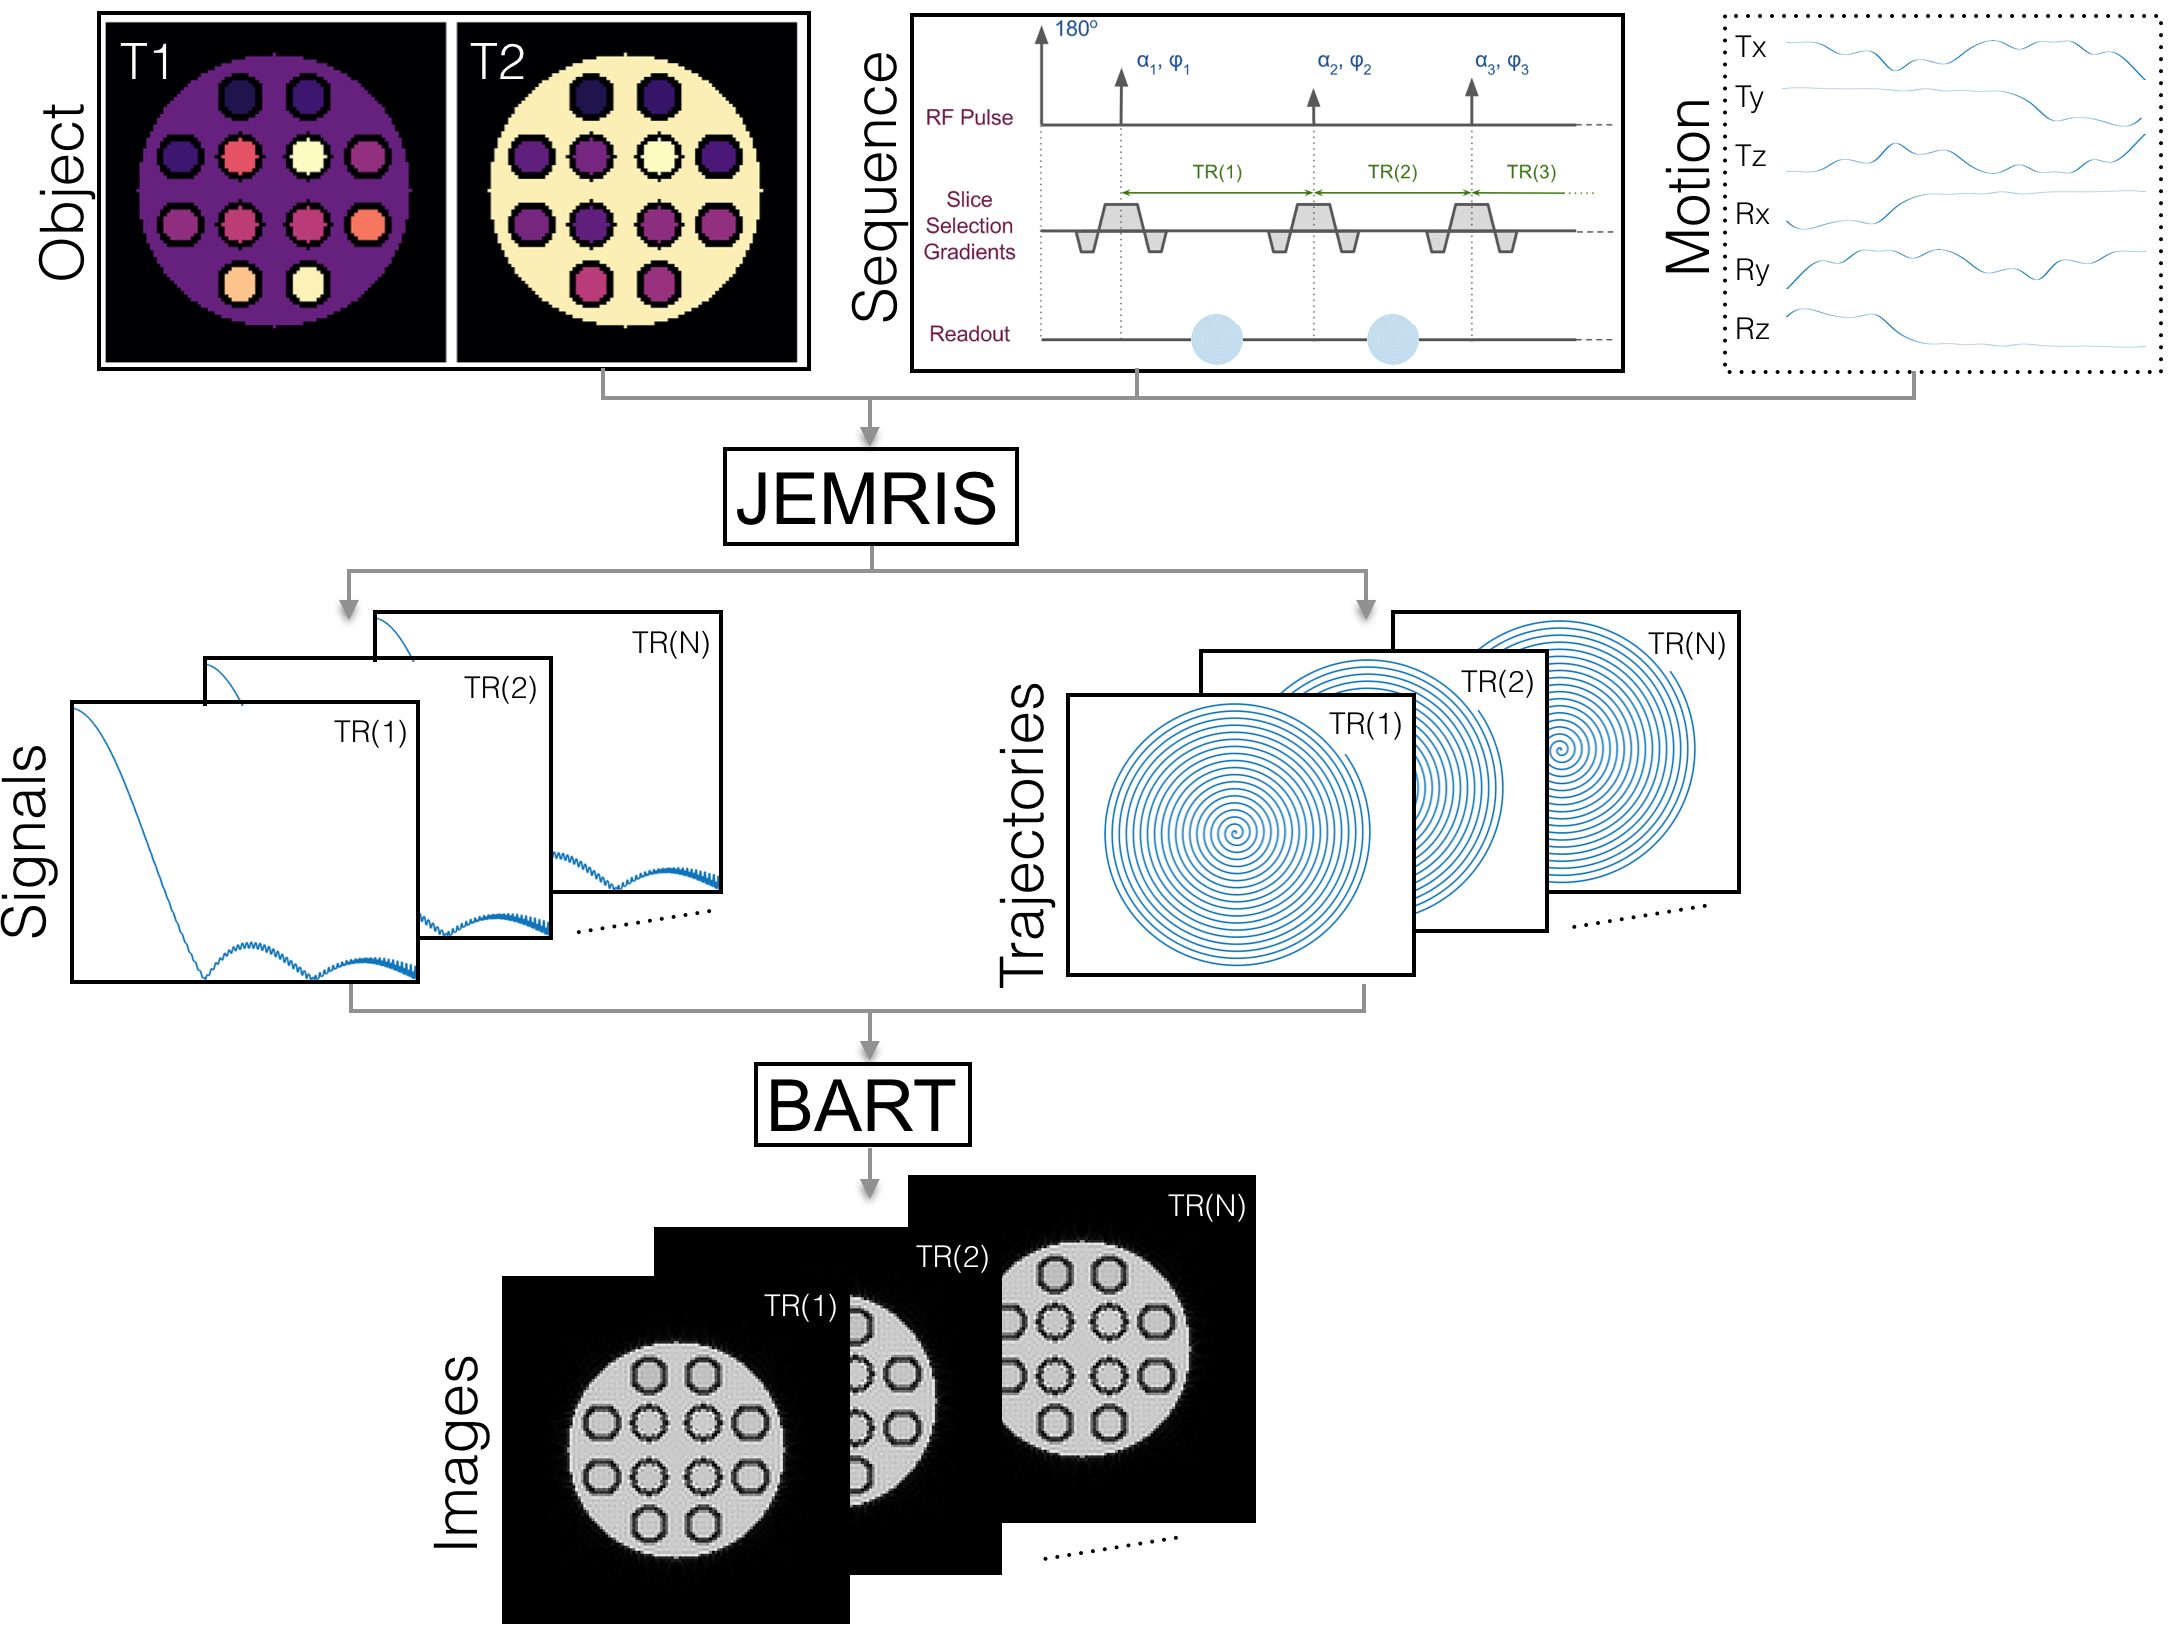
\includegraphics[angle=0,width=1\textwidth, keepaspectratio]{images/mrf/pipelineWithMotion}
%     \caption{Summary of the pipeline used to simulate the images}
%     \label{fig:pipeline}
% \end{figure}

\hfill

% % % % % % % % % % % % % % % % % % % % % % % % % % % % % % % % % % % % % % % % % % % % % % % % % % % % % % % % % % % % % % % % % % % % % % % % % % % % % % % % % % % % % % % % % % % % % % % % % % % % % % % % % % % % % % % % % % % % % % % % % % % % % % % % % % % % % % % % % % % % % % % % 
\subsection{Matching Algorithm}
\label{method:matching}

The pattern matching algorithm used is the same as described in the original MRF implementation \cite{Ma2013}.
It involves a vector dot-product between all the simulated image-space signals and the precomputed dictionary, and the retrieval of the dictionary signal which gives the highest score.
Prior to computing the dot-product, both types of signals are normalised to each having the same sum squared magnitude.
%Conceptually, the two signals need to be as `similar' as possible to say that a certain pair of tissue properties can be attributed to the observed signal.

\hfill

Mathematically, this can be described with the following formulation.
Let there be a dictionary $D \in \mathfrak{C}^{M \times N}$, where M is the number of parameter combinations and N is the number of timepoints.
Any dictionary signal $d_j$, with $j \in [1,M]$, represents the $j^{th}$ row of $D$.
Then, the process of pattern matching involves finding the dictionary entry $d_l$ which satisfies:
\begin{equation}
    d_l = \arg\!\max_{d_j} \, \lvert d_j \, x^* \rvert
\end{equation}
where $x$ is the image-space signal and $x^*$ is the conjugate transpose of $x$.
Both the dictionary entry and the image space signal have to be normalised to have unit length: $\lvert \lvert x \rvert \rvert = \lvert \lvert d_j \rvert \rvert = 1$, where $\lvert \lvert \, \cdot \, \rvert \rvert$ is the Euclidean norm.
Once the match is recovered, the voxel corresponding to the image space signal $x$ is assigned the tissue parameters used to generate the matching entry's signal.

\hfill

This process is then repeated for all the image space signals corresponding to all the voxels in the image dataset.
At the end, a set of tissue parameter maps is created.

% % % % % % % % % % % % % % % % 
\section{Results}\label{chapterlabel3sec3}

This section is focused on showing the main results of my investigation.
I start with discussing the dictionary of generated signals, 
then I move on to showing the results for motion-free simulations,
and I finalize with a discussion about the motion corrupted datasets.

% % % % % % % % % % % % % % % % % % % % % % % % % % % % % % % % % % % % % % % % % % % % % % % % % % % % % % % % % % % % % % % % % % % % % % % % % % % % % % % % % % % % % % % % % % % % % % % % % % % % % % % % % % % % % % % % % % % % % % % % % % % % % % % % % % % % % % % % % % % % % % % % % % % % % % % % % % % % % % % % % % % % % % % % 
\subsection{Dictionary Results}

Two sets of dictionaries were generated using the methods described in Section~\ref{method:dictionary}.
The acquisition sequence consisted of $N = 500$ repetition blocks, with both the repetition time and the echo time kept constant: $T_R = 15ms$ and $T_E = 7.5ms$.
The only sequence parameters that were varied from one acquisition to the next were the flip angles.
Figure~\ref{fig:FAsMaryia} shows the flip angles used for simulating the MRF dictionaries. 
% As the long term goal of my PhD project is to simulate the MRF-FISP sequence, I have chosen the shape of the flip angle distribution according to an MRF-FISP acquisition sequence which was used to acquire MRF data in a real experiment.

\begin{figure}[ht]
    \centering
    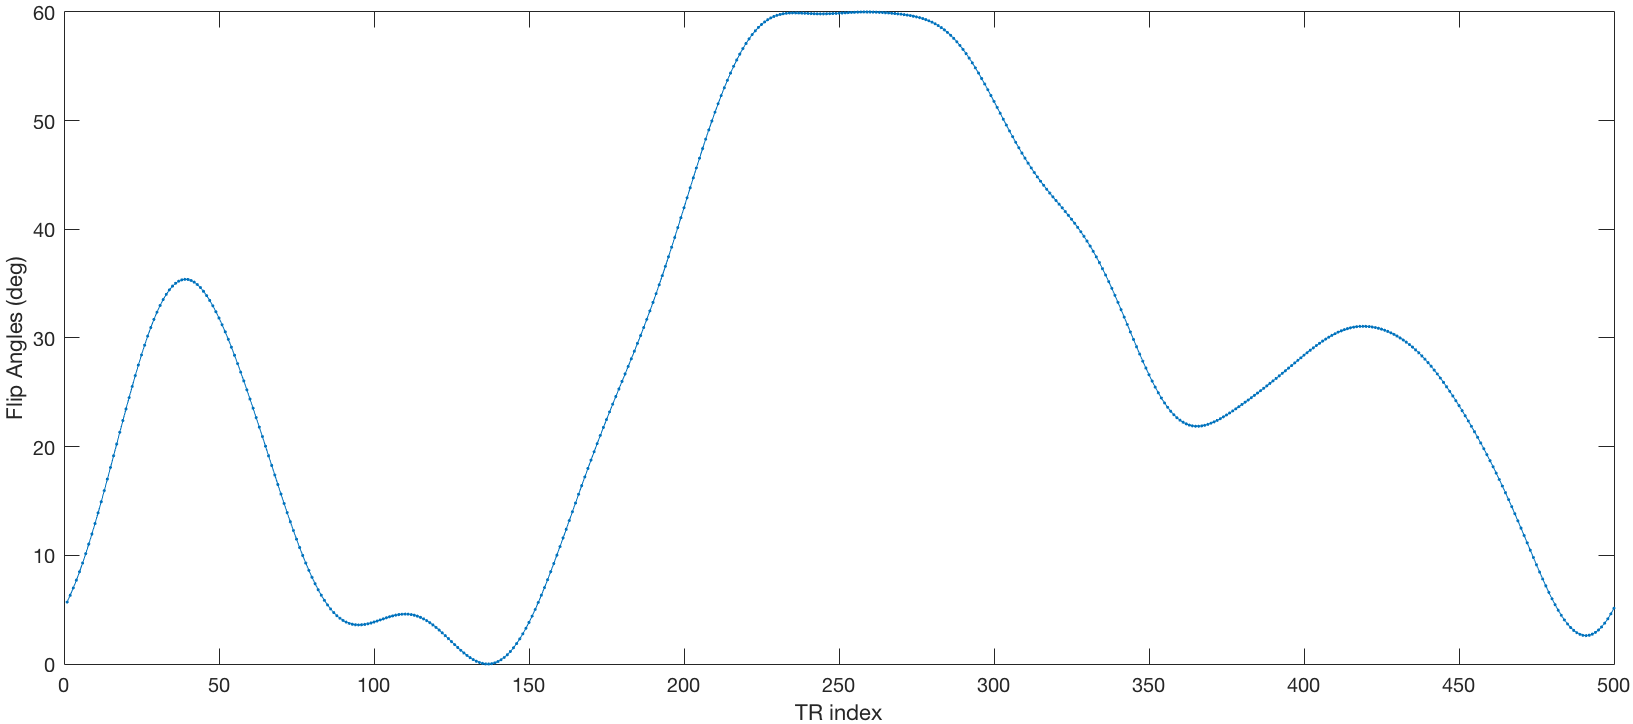
\includegraphics[width=1\textwidth]{images/mrf/FAsMaryia}
    \caption{The flip angles used for simulating the MRF dictionaries.
    The inversion pulse at the beginning of the RF pulse train is not shown here.}
    \label{fig:FAsMaryia}
\end{figure}

\hfill

The ranges of $T_1$ and $T_2$ values for this study were chosen to cover a wide range of typical relaxation times of the TO5 phantom.
Thus, $T_1$ values were chosen between $100ms$ and $2000ms$ with a $5ms$ increment, while
% $T_2$ values were chosen between $20ms$ and $200ms$ with a $5ms$ increment and between $350ms$ and $400ms$ with a $10ms$ increment.
% By applying both methods, two dictionaries, each consisting of $15,843$ entries with $500$ time points, were generated.
$T_2$ values were chosen between $20ms$ and $200ms$ with a $5ms$ increment and between $210ms$ and $400ms$ with a $10ms$ increment.
By applying both methods, two dictionaries, each consisting of $20,687$ entries with $500$ time points, were generated.
A set of representative dictionary entries are shown in Figure~\ref{fig:mrfDictionaries} with a),c) $T_1$ values ranging from $200ms$ to $800ms$ with $100ms$ increment and $T_2$ fixed to $20ms$; and b),d) $T_2$ values ranging from $20ms$ to $80ms$ with $10ms$ increment and $T_1$ fixed to $100ms$.
Next, I will describe some of the key features of the simulated signals.

\begin{figure}[ht]
    \centering
    \begin{subfigure}[b]{.75\textwidth}
        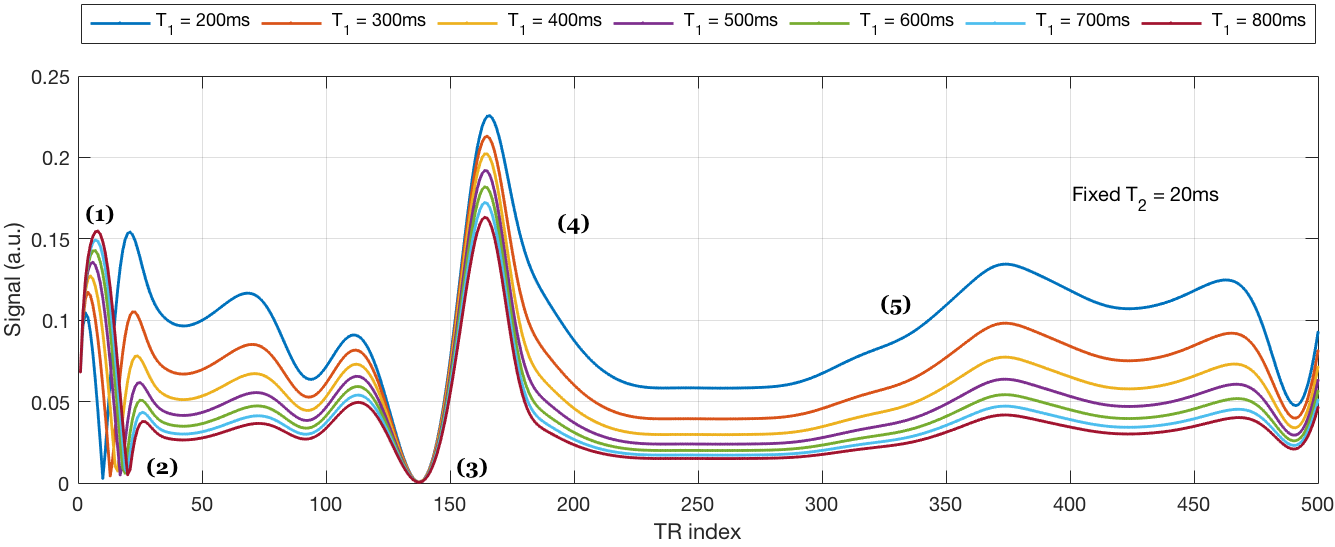
\includegraphics[width=\textwidth]{images/mrf/mrfDictionaryBSSFPaDesc}
        \caption{bSSFP fixed $T_2 = 20ms$}
    \end{subfigure}
    
    \begin{subfigure}[b]{.75\textwidth}
        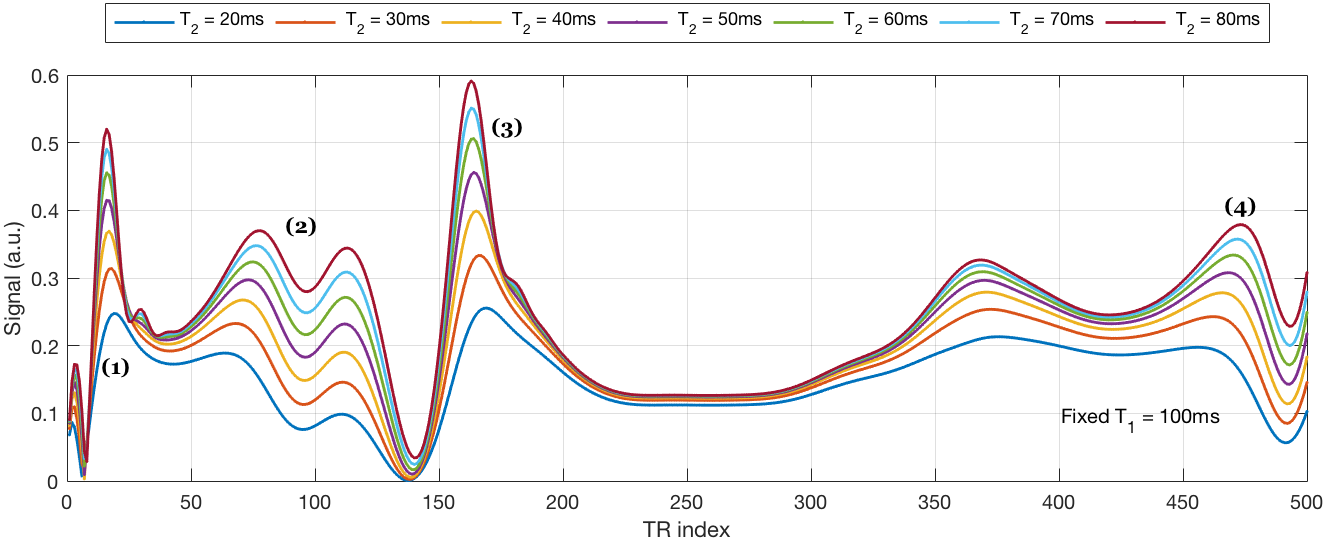
\includegraphics[width=\textwidth]{images/mrf/mrfDictionaryBSSFPbDesc}
        \caption{bSSFP fixed $T_1 = 100ms$}
    \end{subfigure}
    
    \begin{subfigure}[b]{.75\textwidth}
        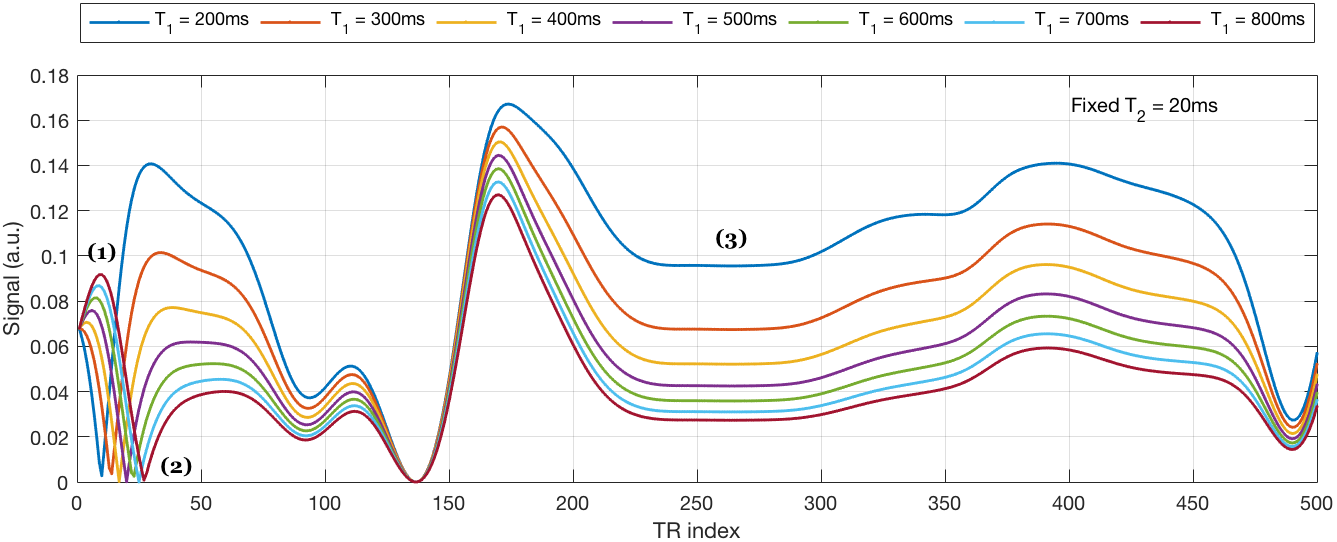
\includegraphics[width=\textwidth]{images/mrf/mrfDictionaryFISPaDesc}
        \caption{FISP fixed $T_2 = 20ms$}
    \end{subfigure}
    
    \begin{subfigure}[b]{.75\textwidth}
        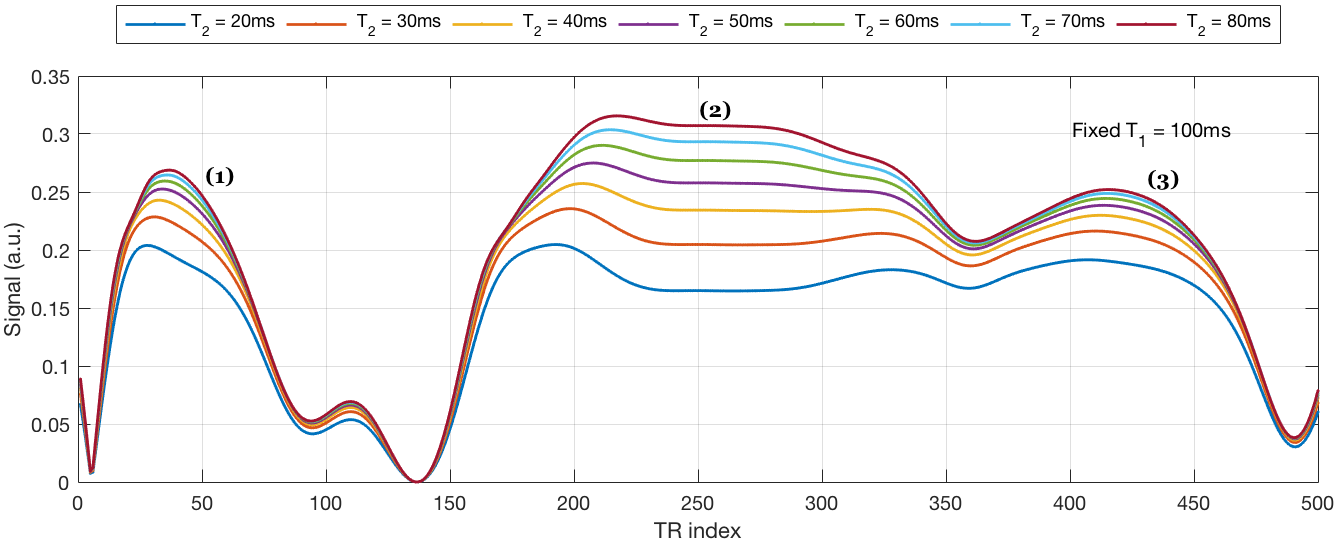
\includegraphics[width=\textwidth]{images/mrf/mrfDictionaryFISPbDesc}
        \caption{FISP fixed $T_1 = 100ms$}
    \end{subfigure}
    
    \caption{Example fingerprints for both the bSSFP and FISP dictionaries. In a) and c) we fix $T_2 = 20ms$ and we vary $T_1$ from $200ms$ to $800ms$ with $100ms$ increment, while in b) and d) we fix $T_1 = 100ms$ and we vary $T_2$ from $20ms$ to $80ms$ with $10ms$ increment.}
    \label{fig:mrfDictionaries}
    % stop checking them against matlab, they ARE FINE!
\end{figure}

\hfill

% % % % Talk about the bSSFP dictionary
\textbf{bSSFP Dictionary.} 
Example fingerprints for the bSSFP dictionary are shown in the first two subplots of Figure~\ref{fig:mrfDictionaries}.
In \textbf{a)} the transverse relaxation time is kept fixed. 
The difference in shape between the fingerprints is due solely to their $T_1$ relaxation times.
The $180^o$ inversion pulse makes the fingerprints more easily distinguishable from the beginning:
a slower longitudinal relaxation rate ($T_1 = 800ms$) means that at the beginning of the sequence there is more magnetisation to be flipped in the transverse plane, while a faster longitudinal relaxation rate ($T_1 = 200ms$) will cause the opposite effect (1).
After a while, as the shorter $T_1$s help the magnetisation vector reach equilibrium faster, these fingerprints will have a stronger contribution to the signal and the signal trends will switch (2).

\hfill

By the $140^{th}$ pulse the flip angle values get closer to $0$. 
As a consequence of that, we can see a lack of signal at the same TR index (3).
This also allows the magnetisation vector to relax and give more signal as the flip angles increase in magnitude (4).
Moreover, as the flip angles are continuously varied, the signal is not allowed to reach steady state, but is kept in its transient phase which also allows for better discrimination throughout the sequence (5).

\hfill

In \textbf{b)} the longitudinal relaxation time is kept fixed and the difference in shapes between these fingerprints is due to their $T_2$ relaxation times.
Now, these signals are better discriminated from each other as the flip angles vary (see (1)-(4)): this keeps the signal in the transient phase and does not allow it to reach steady state.
Moreover, a slower transverse relaxation rate ($T_2 = 80ms$) will allow for more signal, while a faster transverse relaxation rate ($T_2 = 20ms$) will have the opposite effect.
This trend is seen throughout the entire acquisition.

\hfill

% % % % Talk about the FISP dictionary
\textbf{FISP Dictionary.} 
Example fingerprints for the FISP dictionary are shown in the last two subplots of Figure~\ref{fig:mrfDictionaries}.
The first feature to be noticed is that these signals have an overall lower magnitude than the ones for bSSFP.
This is a known consequence of using dephasing gradients and is explained in Appendix \ref{MRIFISP}.

\hfill

In \textbf{c)} the transverse relaxation time is kept fixed. 
Same as before, the difference in shapes between the fingerprints is due to their $T_1$ relaxation times and the $180^o$ inversion pulse which make the fingerprints more easily distinguishable at the beginning (1).
After some time, as the magnetisation vector relaxes towards thermal equilibrium and becomes positive, the signal trends flip (2).
From this moment on, throughout the entire sequence, the faster longitudinal relaxation rate ($T_1 = 200ms$) will give the higher signal, while the slowest longitudinal relaxation rate ($T_1 = 800ms$) will give the lowest signal (3), as expected.

\hfill

In \textbf{d)} the longitudinal relaxation time is kept fixed and, as before, the difference in shapes between the fingerprints is due to their $T_2$ relaxation times.
Now, throughout the sequence, the higher $T_2$ values will give higher signal than the lowest $T_2$ values.
This is because the magnetisation vector will relax slower for the higher values and faster for the lower values by the readout time.
Moreover, these signals are better discriminated from each other as the flip angles get bigger (see (1)-(3), where $FA \geq 30^o$).
This is expected as very small flip angles will cause less magnetisation to be tipped in the transverse plane.

\hfill

For the remainder of this work I am only using the bSSFP dictionary.
This is because the image space simulations are done using a balanced steady state sequence.
The FISP sequence requires more computational power and it is in my future work.
Next, I will discuss the motion free and motion corrupted results.

% % % % % % % % % % % % % % % % % % % % % % % % % % % % % % % % % % % % % % % % % % % % % % % % % % % % % % % % % % % % % % % % % % % % % % % % % % % % % % % % % % % % % % % % % % % % % % % % % % % % % % % % % % % % % % % % % % % % % % % % % % % % % % % % % % % % % % % % % % % % % % % % % % % % % % % % % % % % % % % % % % % % % % % % 
\clearpage
\subsection{Image Space Simulations Results}

Ten different quantitative maps were generated using the methods described in Sections \ref{method:imagespace} and \ref{method:matching}, corresponding to one motion free dataset and 9 motion corrupted datasets.
The acquisition scheme was a balanced steady state free precession sequence with $N = 500$ repetition blocks, and constant $T_R = 15ms$ and $T_E = 7.5ms$.
Similar to the dictionary generation part, the only sequence parameters that were varied from one acquisition to the next were the flip angles (Figure~\ref{fig:FAsMaryia}).
Images from each acquisition block were reconstructed separately on an $128 \times 128$ matrix size using BART's \textsc{nufft} command line tool.
Then, a vector dot product was performed between the image space signals corresponding to every voxel position in the image dataset and the entire bSSFP dictionary.
Quantitative maps were created following the method described in Section \ref{method:matching}.

% T1/T2/Score maps no motion vs ground truth
\begin{figure}[ht]
    \centering
    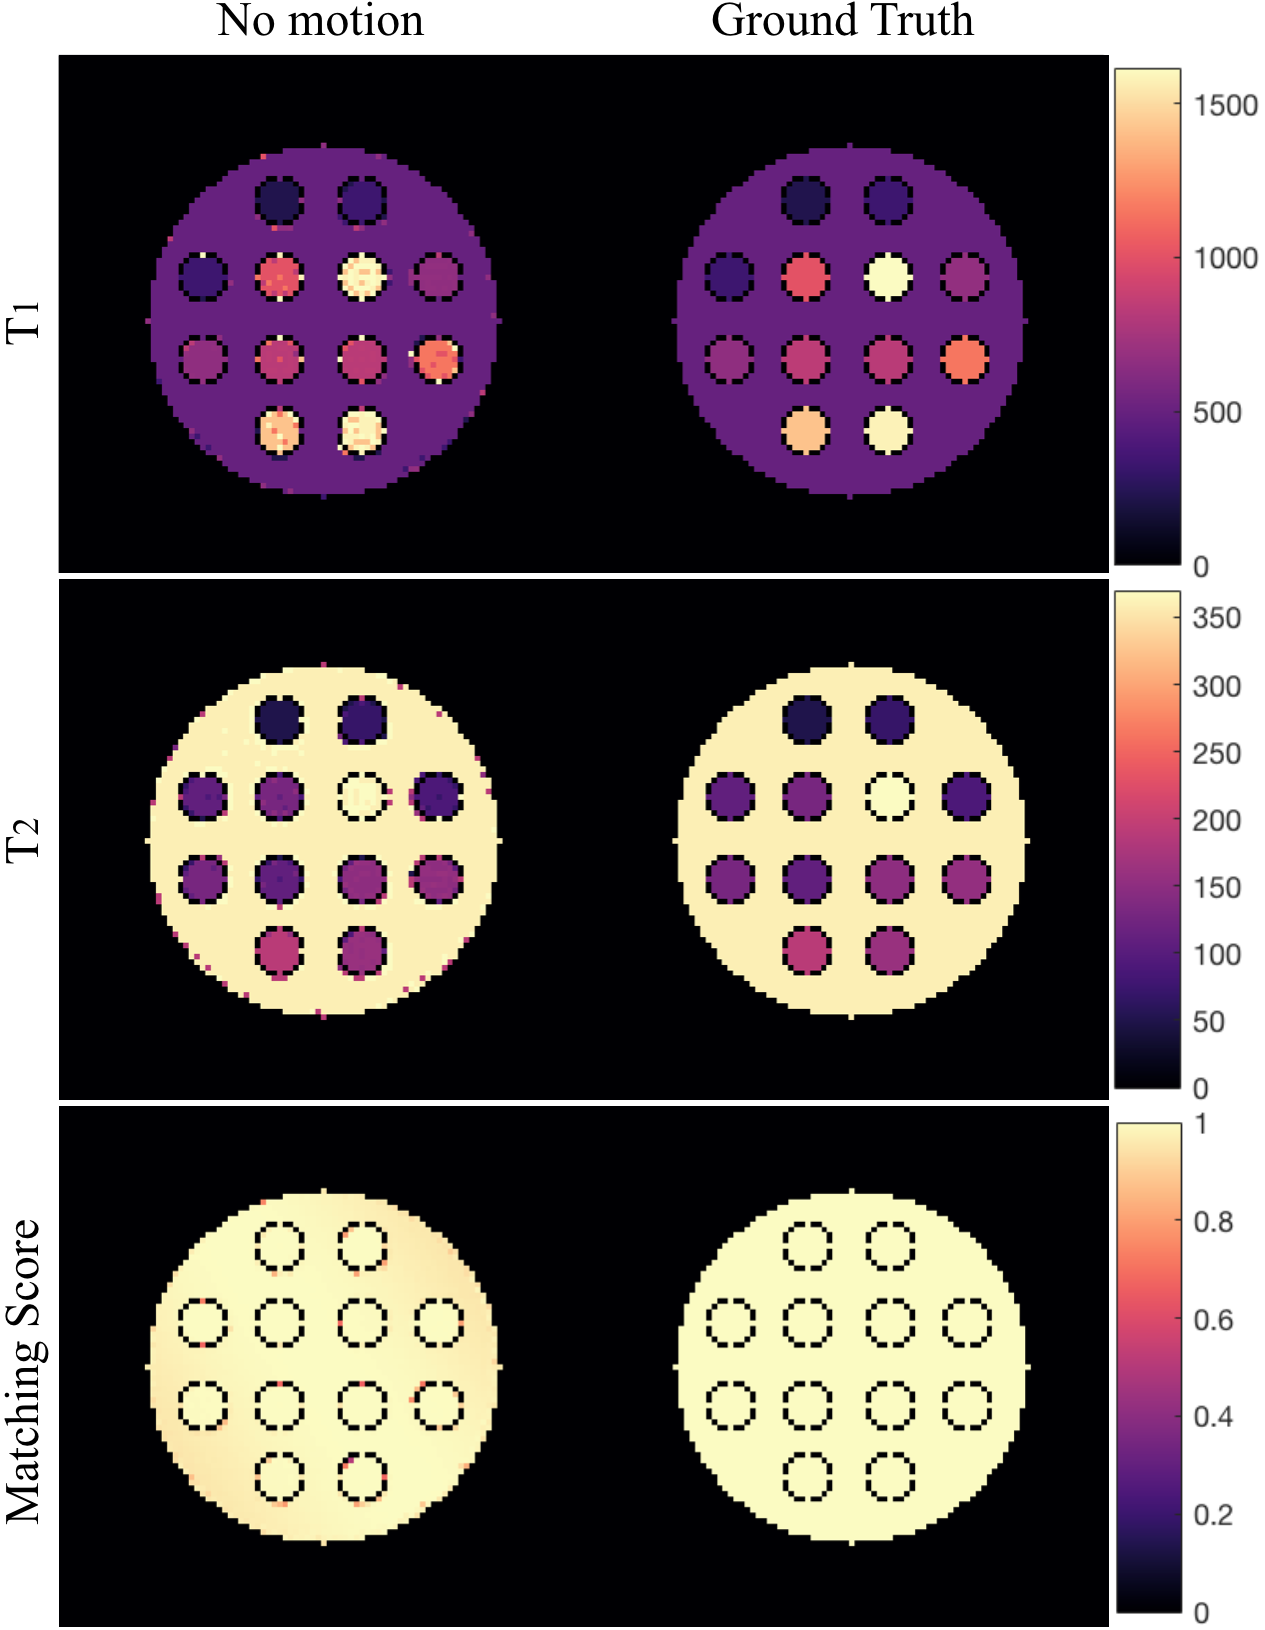
\includegraphics[width=0.6\textwidth]{images/mrf/T1T2ScoreNoMotion}
    \caption{$T_1$ and $T_2$ reconstructed maps together with the matching scores (column 1) and their corresponding ground truth values (column 2).}
    \label{fig:T1T2ScoreMapNoMotion}
\end{figure}

% % % % % % % % % % % % % % % % 
\subsubsection{Motion Free Results}
The first set of results corresponds to the motion free simulations.
These maps are shown in Figure~\ref{fig:T1T2ScoreMapNoMotion} where a mask was introduced to both eliminate the noise surrounding the object and to better distinguish the inner tubes from the bigger circle.
The results show that the reconstructed $T_1$ and $T_2$ maps are in good agreement with the ground truth values.
Moreover, the voxel-wise pattern matching scores are above 0.95 everywhere inside the reconstructed object.

\hfill

Figure~\ref{fig:nomotionExampleSignals} shows two examples of image space signals and their corresponding dictionary match.
Both matching scores are very high and the retrieved fingerprints correspond to the ground truth values. 

\begin{figure}[H]
    \centering
    \begin{subfigure}[b]{.7\textwidth}
        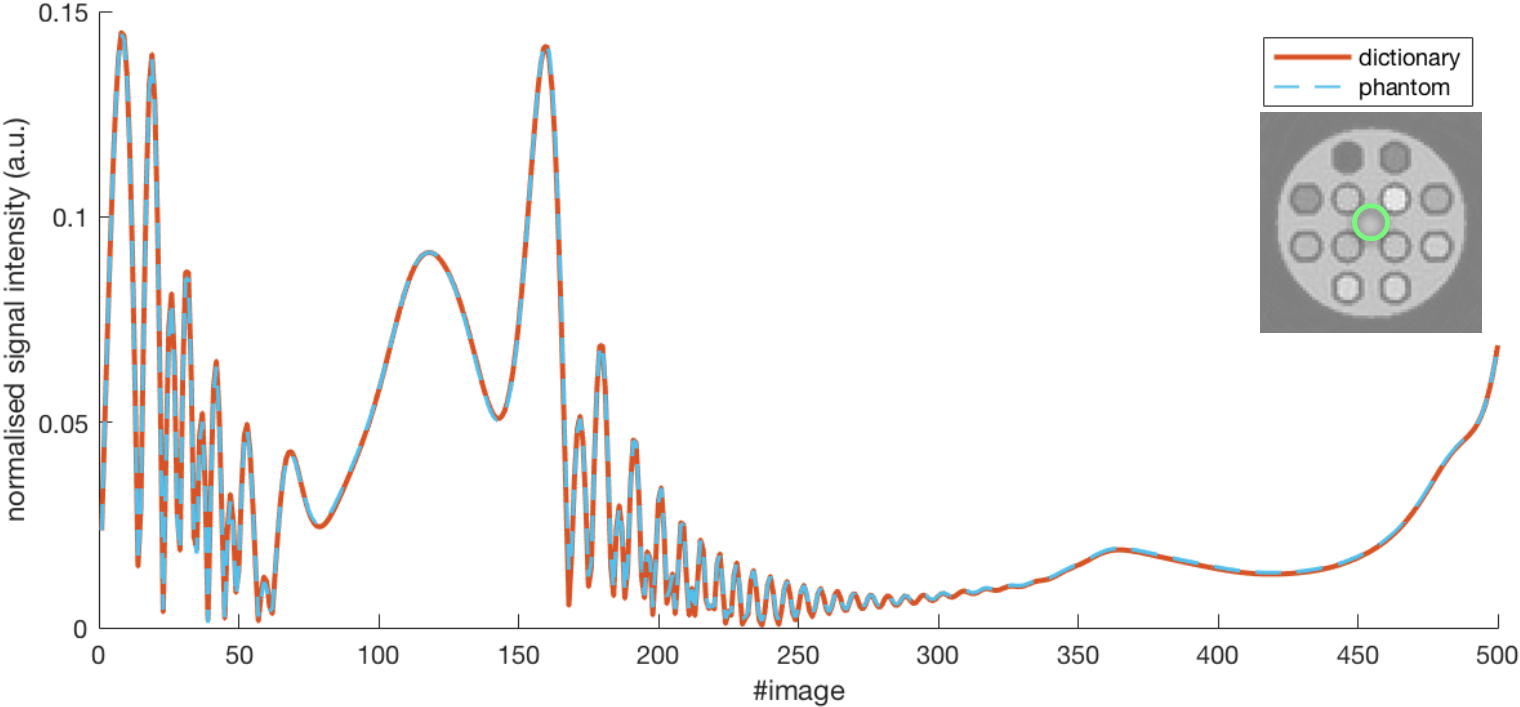
\includegraphics[width=\textwidth]{images/mrf/nomotionExampleSignalsa}
        \caption{The image space signal (blue dashed) matched to the fingerprint (red) corresponding to $T_1 = 500ms$ and $T_2 = 360ms$, with a matching score of 0.99.}
    \end{subfigure}
    
    \begin{subfigure}[b]{.7\textwidth}
        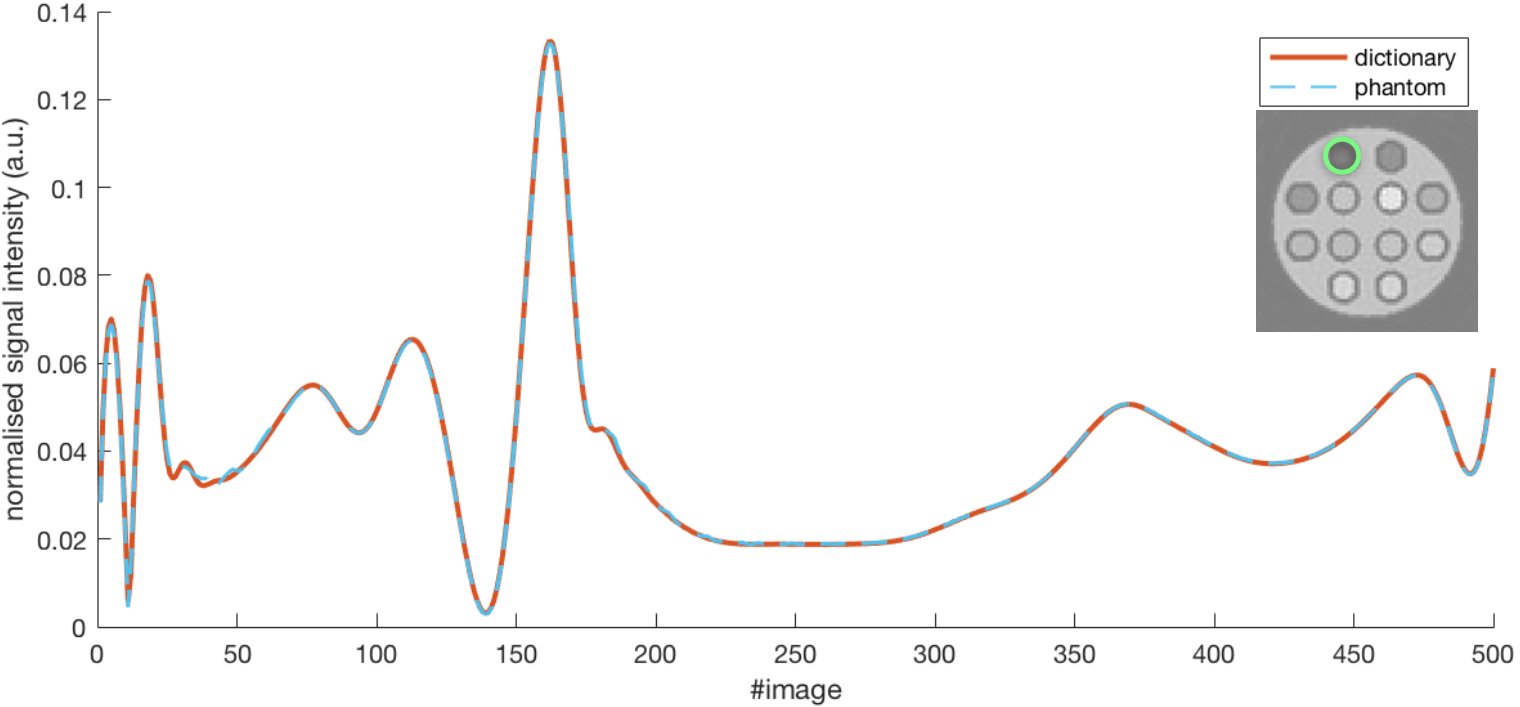
\includegraphics[width=\textwidth]{images/mrf/nomotionExampleSignalsb}
        \caption{The image space signal (blue dashed) matched to the fingerprint (red) corresponding to $T_1 = 225ms$ and $T_2 = 50ms$, with a matching score of 0.99}
    \end{subfigure}
    
    \caption{Example of image space signals matched to dictionary fingerprints for two different places within the phantom.
    Both results retrieve the correct ground truth values.}
    \label{fig:nomotionExampleSignals}
\end{figure}


% % % % % % % % % % % % % % % % 
\subsubsection{Motion Corrupted Results}

The second set of results corresponds to the motion corrupted simulations.
These maps are shown in Figure~\ref{fig:T1mapsmotion} and in Figure~\ref{fig:T2mapsmotion}, while the corresponding matching scores are in Appendix~\ref{appendixlabelMotion}.
Again, a mask was applied to eliminate the noise surrounding the object.

\hfill

The results show that, despite of the motion, the morphological structures of the phantom are well preserved in the $T_1$ and $T_2$ maps. 
However, the surrounding areas around each tube do not show the same sharpness as before.
Qualitatively, both $T_1$ and $T_2$ maps seem to be most affected when motion happens at the beginning of the scan, while the least affected maps are those when motion happens in the middle of the scan.

\hfill

To quantify the deviations from the ground truth values, I performed a region of interest analysis.
This consisted of calculating the mean $T_1$ and $T_2$ values obtained in each of the simulated inner tubes of the digital phantom,
in both the motion free and the motion corrupted data set and comparing them to the ground truth values.
The difference in absolute value between the simulated values and the ground truth values are shown in Figure~\ref{fig:GTMinusSimuAbsoluteDifference} for both the $T_1$ maps and the $T_2$ maps (see also Figures \ref{fig:appendixmotion1ROI}, \ref{fig:appendixmotion2ROI} and \ref{fig:appendixmotion3ROI}).

\hfill

The first important feature to observe in these results is that the region of interest positioned in the middle of the phantom is least affected by the motion.
This is to be expected for motion happening at any time point during the scan as the rotation's axis is going through this middle point and the translation is happening along a line which does not intersect any other structures.
Next, the figure also shows that the reconstructed $T_1$ values are affected the most when the motion happens in the beginning or at the end of the scan, while the $T_2$ values are effected the most when the motion happens at the beginning of the scan.

\hfill

The most affected reconstructed values correspond to the $5^{th}$ tube for both $T_1$ and $T_2$ values, and for the $5^{th}$, the $11^{th}$ and the $12^{th}$ tubes for the $T_1$ values.
To understand why, I plot in Figure~\ref{fig:problematicfingerprints} the dictionary fingerprints corresponding to $T_1$ and $T_2$ values which are close to the problematic tubes.
Moreover, I highlight the areas where the motion is happening for the three different onsets.
When $T_2$ is fixed, the fingerprints are very close together, especially in the middle of the sequence.
This explains why the $T_1$ maps are mostly affected when motion happens in the beginning of the sequence as that is the point where the dictionary match carries more significance.
Also, the last 50 repetition blocks in the sequence show a `spread' in the signals, which can explain why the $T_1$ maps can also be affected when motion is happening at the end of the scan.
When $T_1$ is fixed, the fingerprints are close together in the middle and at the end, which explains why it is more important that the signals are matched correctly at the beginning of the scan and why the $T_2$ maps are mostly affected when that happens.

\begin{figure}[ht]
    \centering
    \begin{subfigure}[b]{.85\textwidth}
        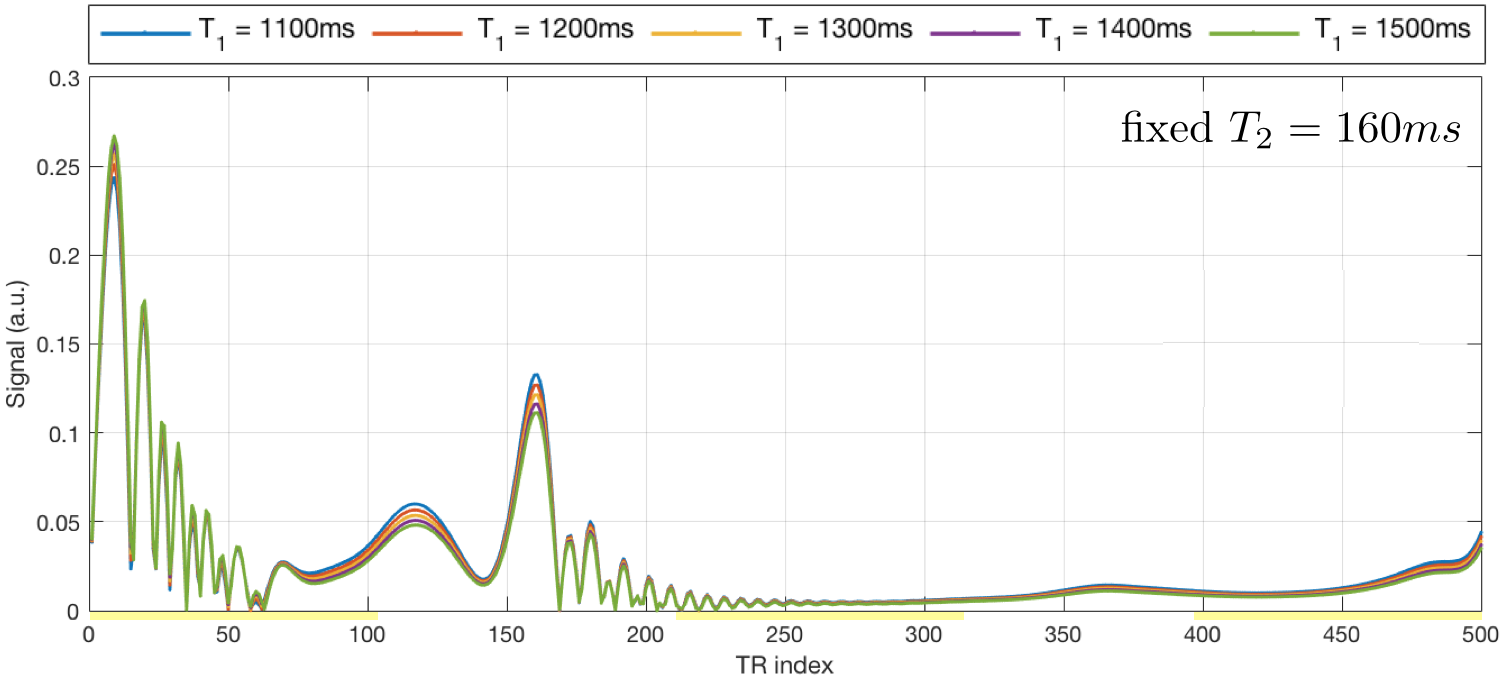
\includegraphics[width=\textwidth]{images/mrf/FixedT2VaryT1TubesMotion}
        \caption{Dictionary fingerprints corresponding to a range of $T_1$ values and a fixed $T_2$ value}
    \end{subfigure}
    
    \begin{subfigure}[b]{.85\textwidth}
        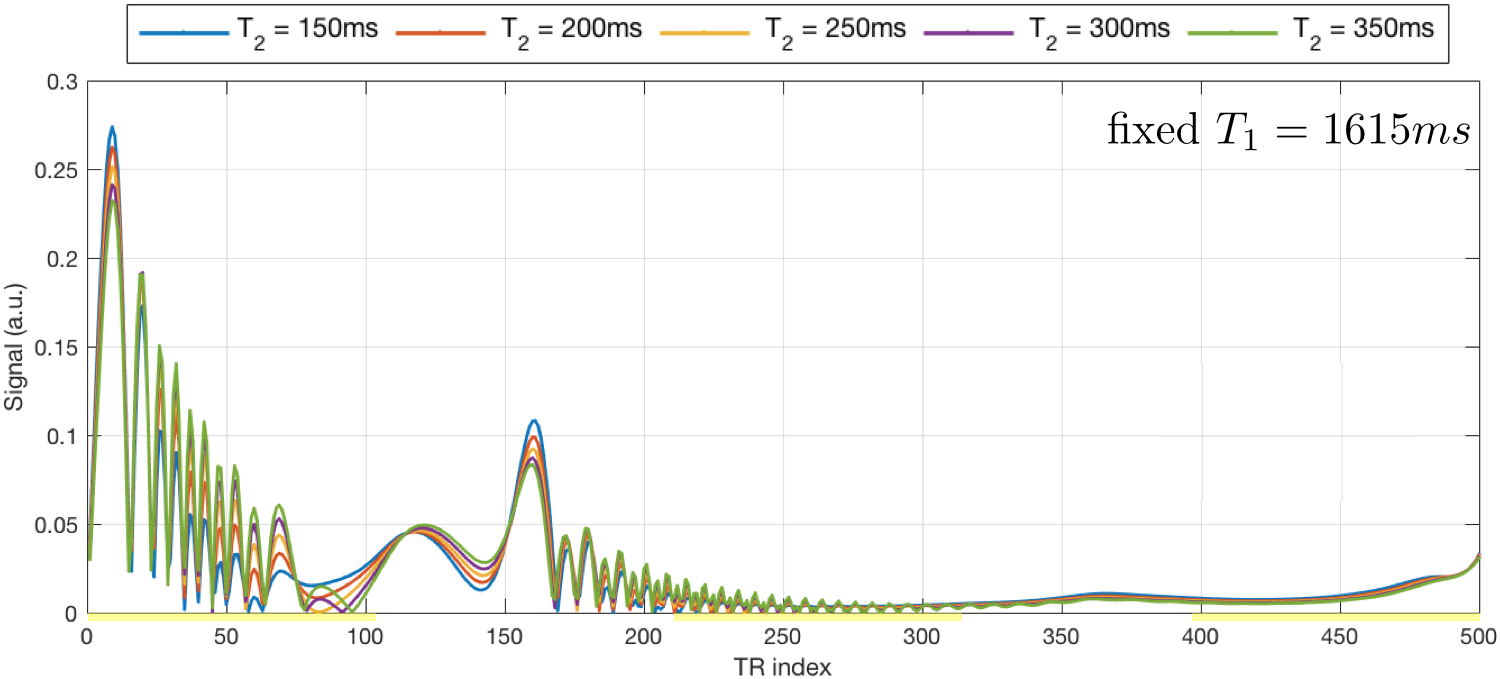
\includegraphics[width=\textwidth]{images/mrf/FixedT1VaryT2TubesMotion}
        \caption{Dictionary fingerprints corresponding to a range of $T_2$ values and a fixed $T_1$ value}
    \end{subfigure}
    
    \caption{Example fingerprints for $T_1$ and $T_2$ values corresponding to the most affected phantom tubes.
    Highlighted areas show when motion is happening.}
    \label{fig:problematicfingerprints}
\end{figure}

% ROI T1 and T2 average all simulated
\begin{figure}[ht]
    \centering
    \begin{subfigure}[b]{.9\textwidth}
        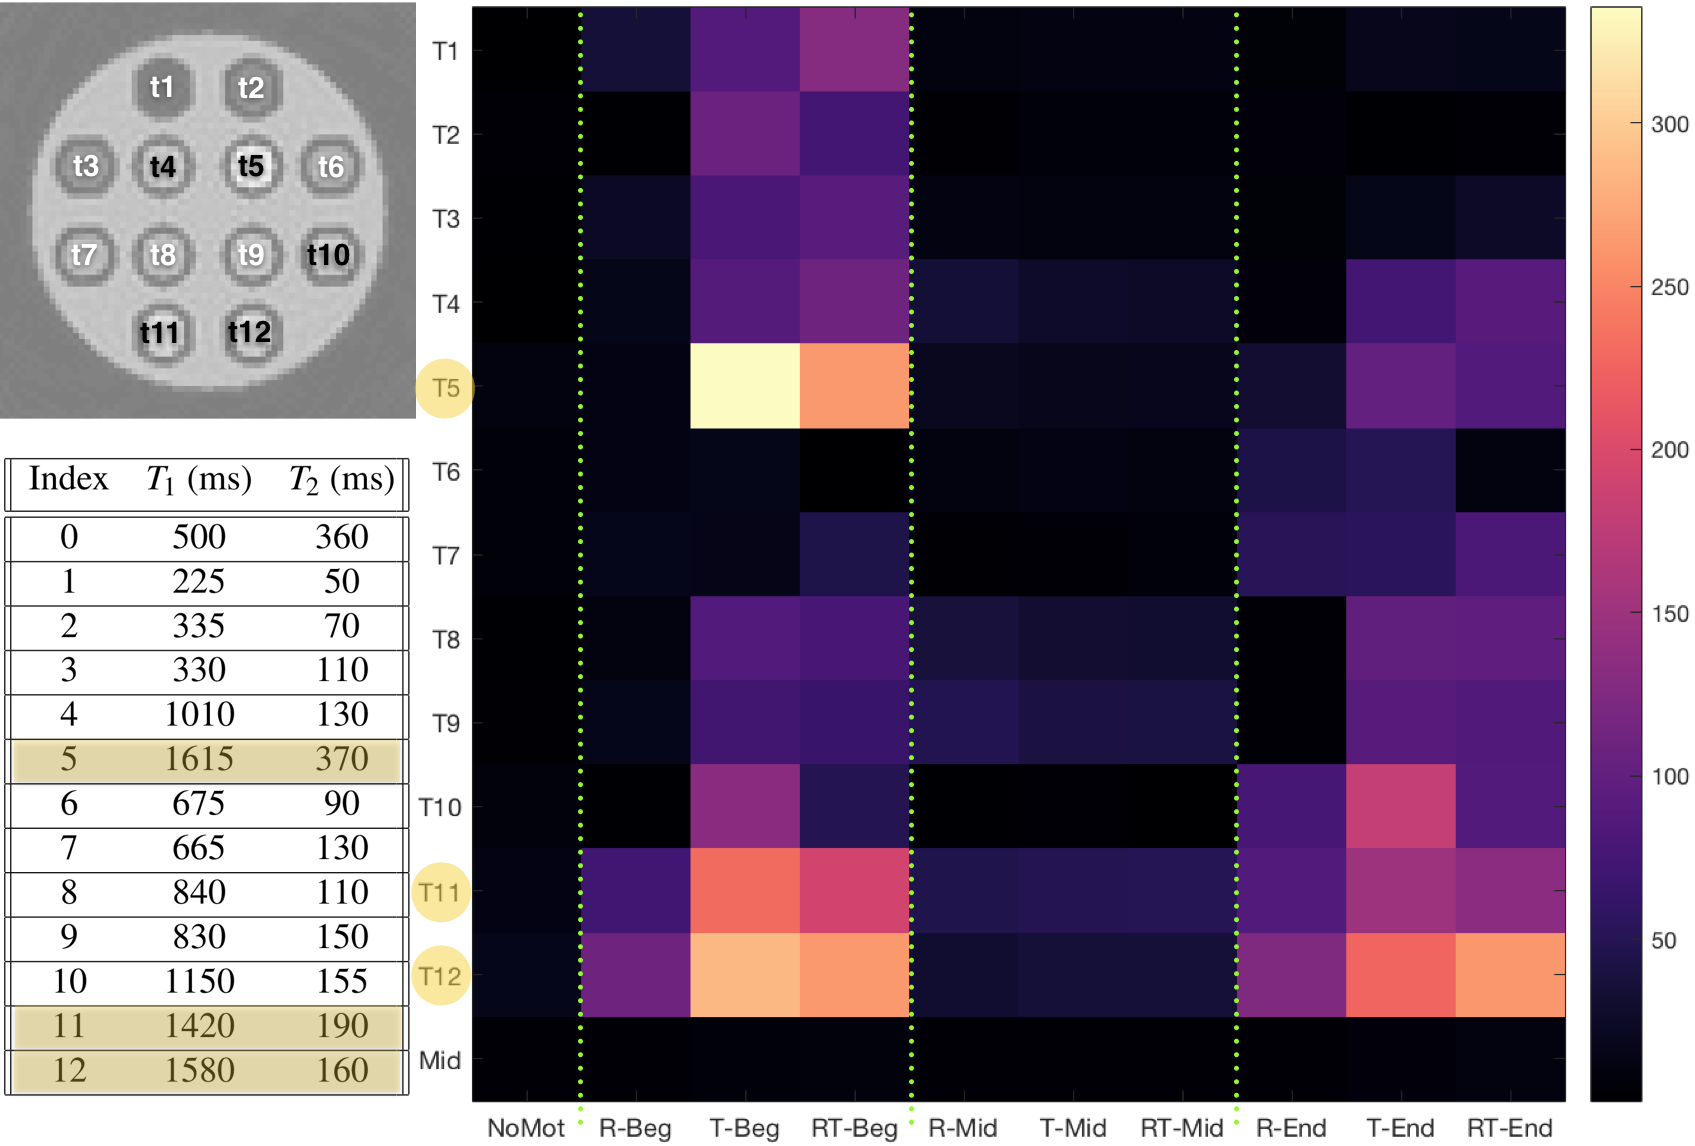
\includegraphics[width=\textwidth]{images/mrf/T1GTMinusT1SimuAbsoluteDifference}
        %\caption{$|T_1^{simulated} - T_1^{ground \, \, truth}|$}
        \label{fig:T1GTMinusT1SimuAbsoluteDifference}
    \end{subfigure}
    
    \begin{subfigure}[b]{.9\textwidth}
        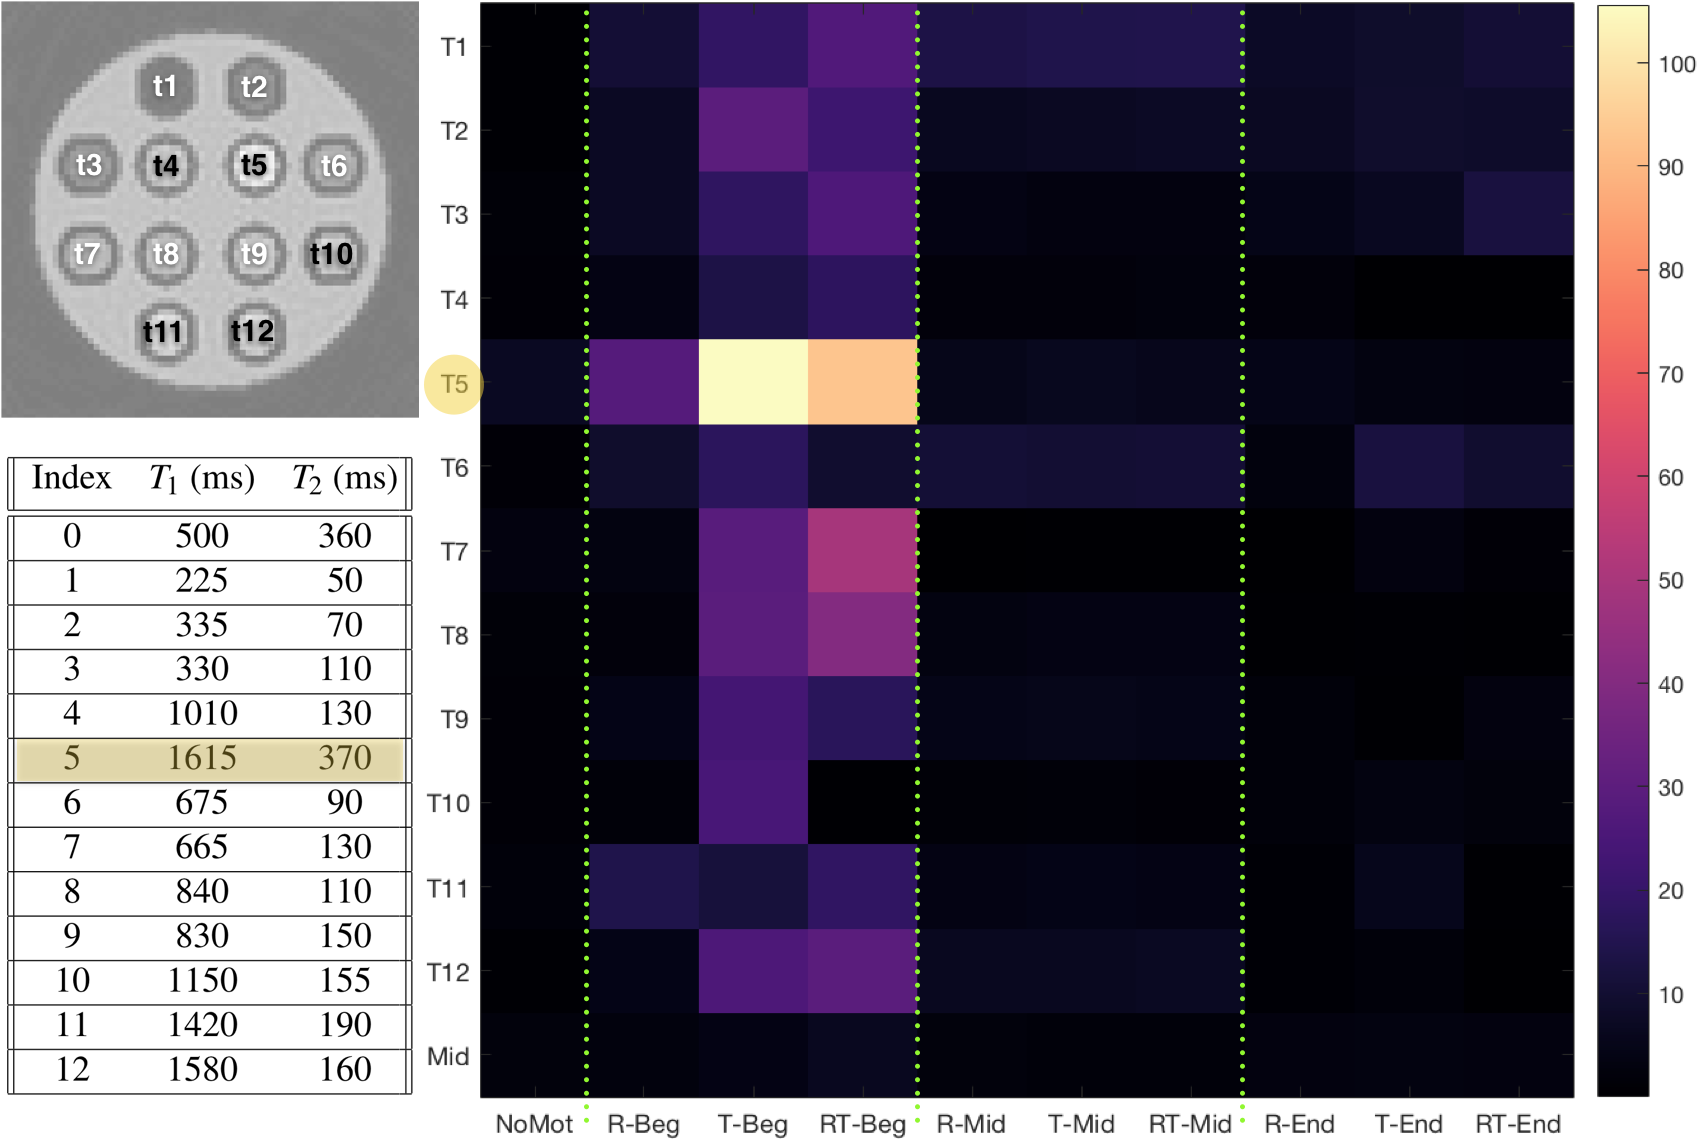
\includegraphics[width=\textwidth]{images/mrf/T2GTMinusT2SimuAbsoluteDifference}
        %\caption{$|T_2^{simulated} - T_2^{ground \, \, truth}|$}
        \label{fig:T2GTMinusT2SimuAbsoluteDifference}
    \end{subfigure}
    
    \caption{Region of interest analysis on the inner tubes (shown as $T_N$ in the plot) and middle of the phantom (shown as $Mid$ in the plot) for the simulated quantitative a) $T_1$  maps and b) $T_2$ maps.
    The plot shows the difference in absolute value between the simulated a) $T_1$ maps or b) $T_2$ maps and the ground truth values.
    Each line corresponds to a different part of the phantom, shown in the upper left corner of the figure, while different columns correspond to different motion types and onsets.
    The first column corresponds to the no motion case,
    while the rest correspond to all three types of motion with onset at:
    the beginning of the scan (first three columns),
    the middle of the scan (next three columns), and
    at the end of the scan (last three columns).
    The ground truth values are found in the table, where the tubes with the highest difference in absolute values for all motion types were highlighted.}
    \label{fig:GTMinusSimuAbsoluteDifference}
\end{figure}

% For this, I chose 4 of the inner tubes, corresponding to the $1^{st}$, $3^{rd}$, $5^{th}$ and $12^{th}$ tube, and also an ROI positioned in the middle of the phantom.
% The results for ground truth, motion free and different onsets of \textit{motion 1} are shown in Figure~\ref{fig:motion1ROI}.
% The other two types of motion are found in Appendix~\ref{appendixlabelMotion}, in Figure~\ref{fig:appendixmotion2ROI} and Figure~\ref{fig:appendixmotion3ROI}.

% % ROI analysis motion 1
% \begin{figure}[ht]
%     \makebox[\textwidth][c]{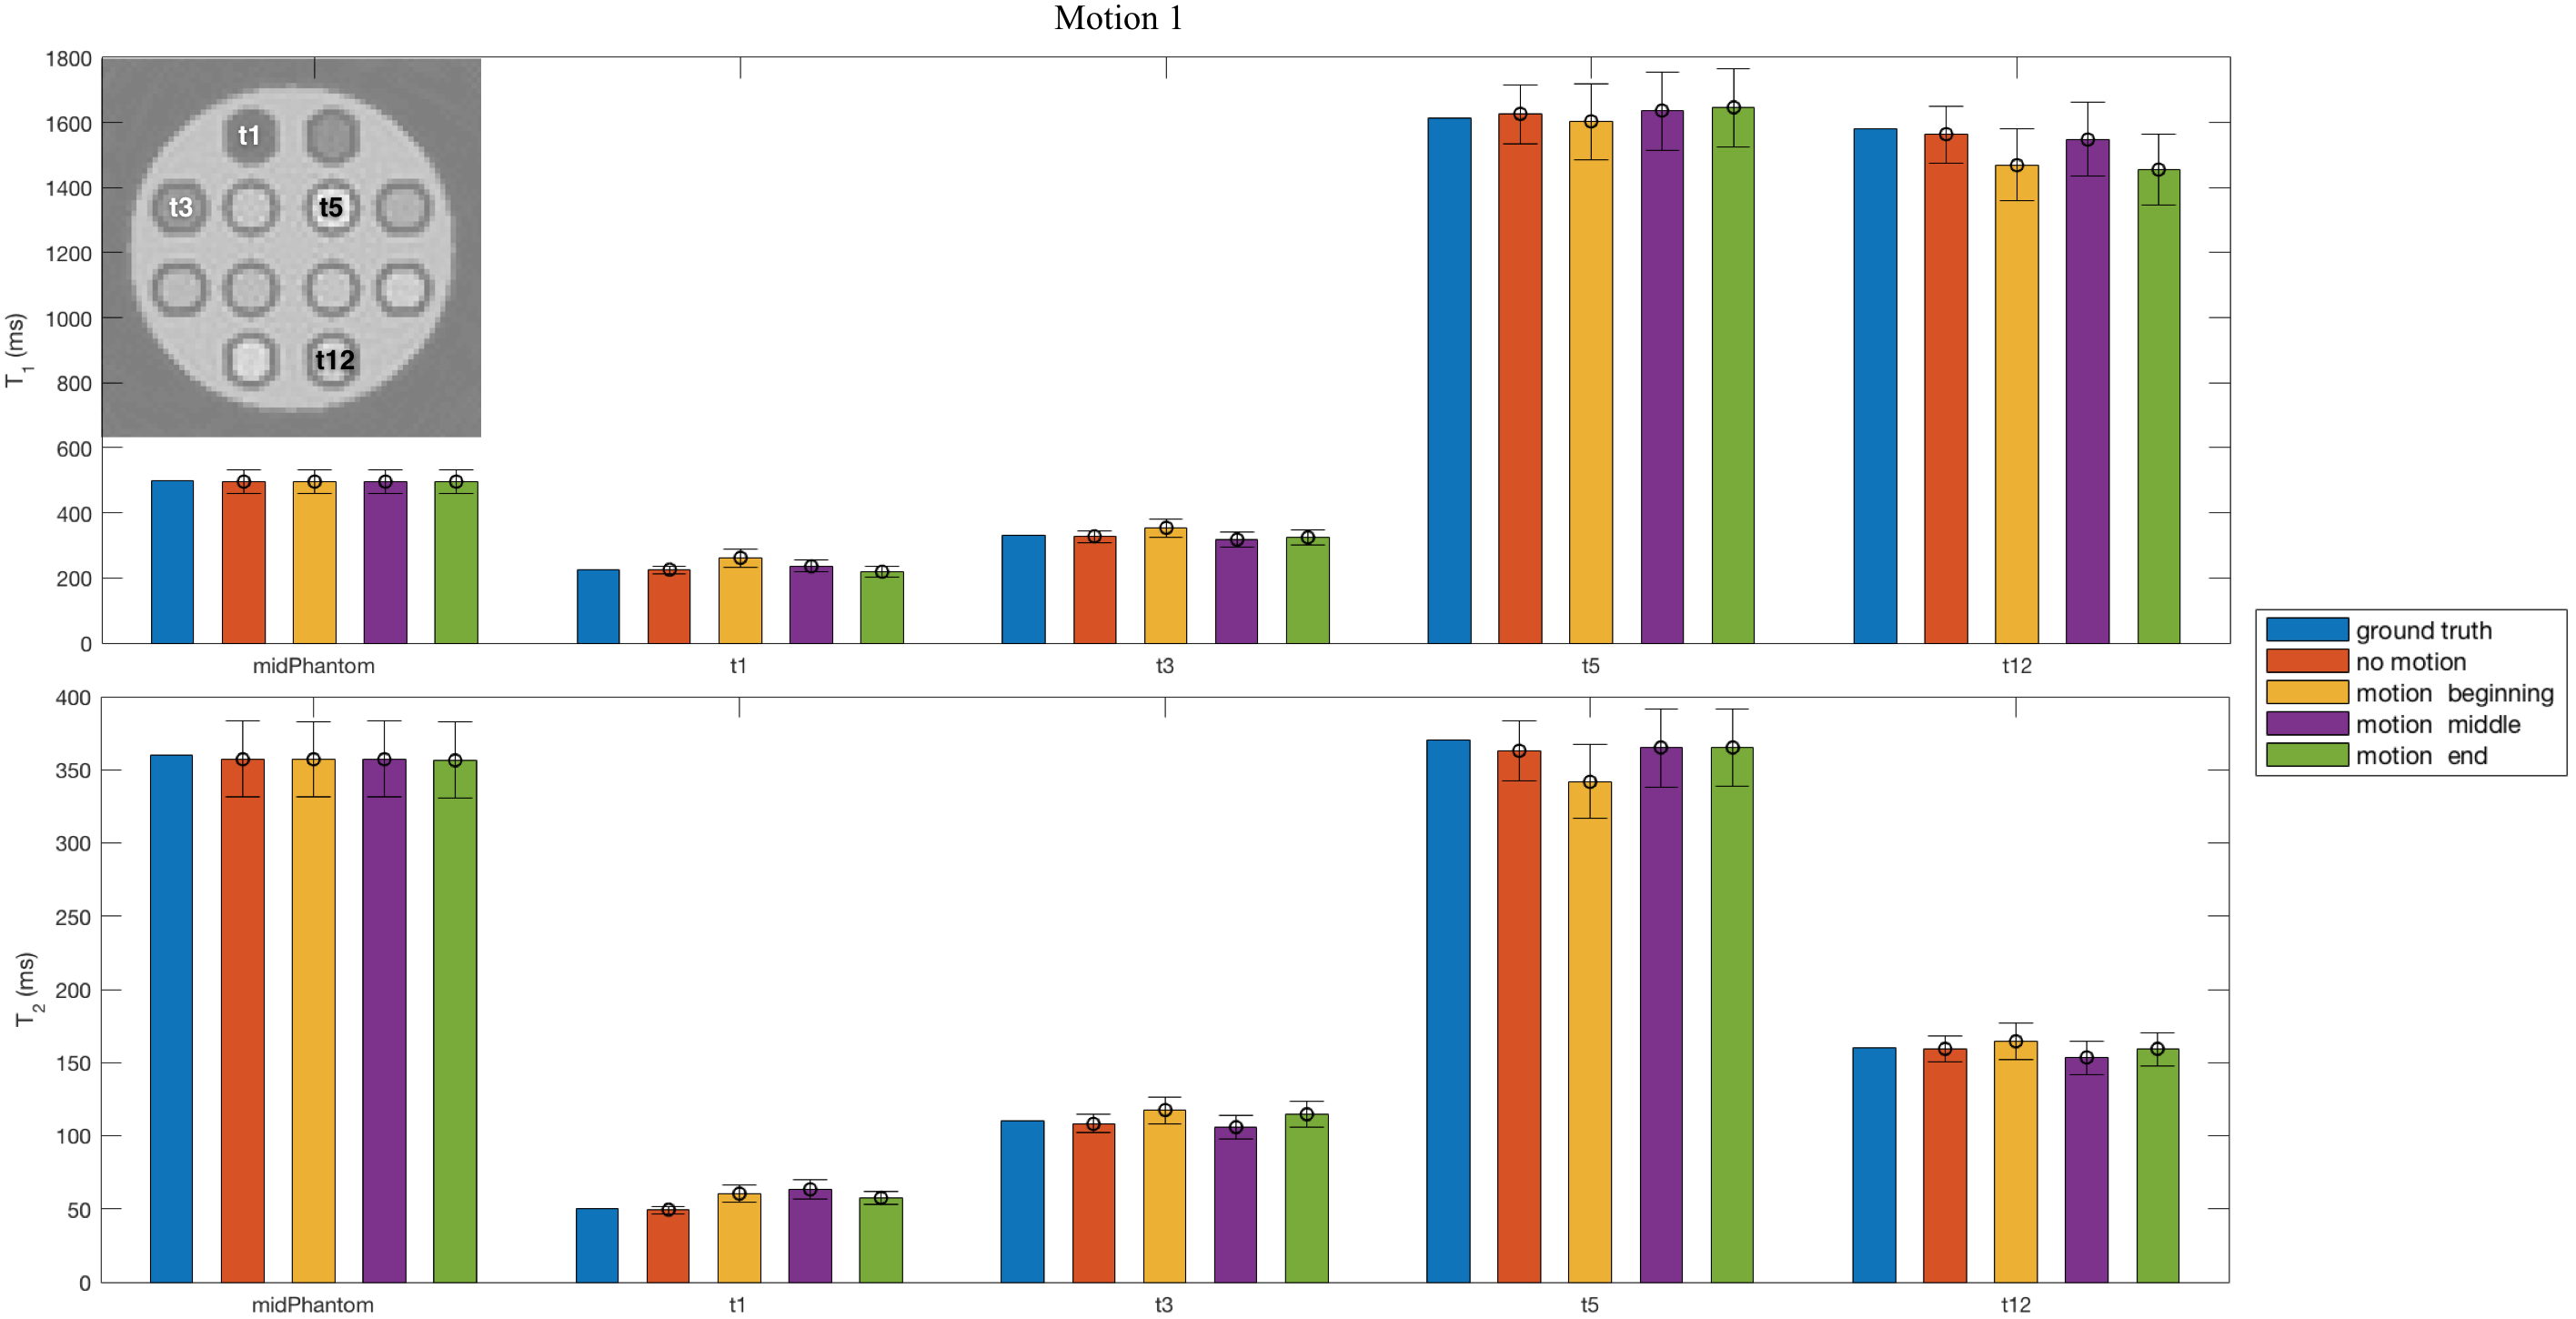
\includegraphics[width=1.3\textwidth]{images/mrf/motion1ROI}}
%     \caption{Region of interest analysis on \textit{motion 1} for different motion onsets}
%     \label{fig:motion1ROI}
% \end{figure}

\hfill

% The first important feature to observe in these results is that the region of interest positioned in the middle of the phantom is least affected by the motion.
% This is to be expected for motion happening at any time point during the scan as the rotation's axis is going through this middle point and the translation is happening along a line which does not intersect any other materials.

% % % Put images here:
% T1 maps motion
\begin{figure}[ht]
    \centering
    \begin{subfigure}[b]{.65\textwidth}
        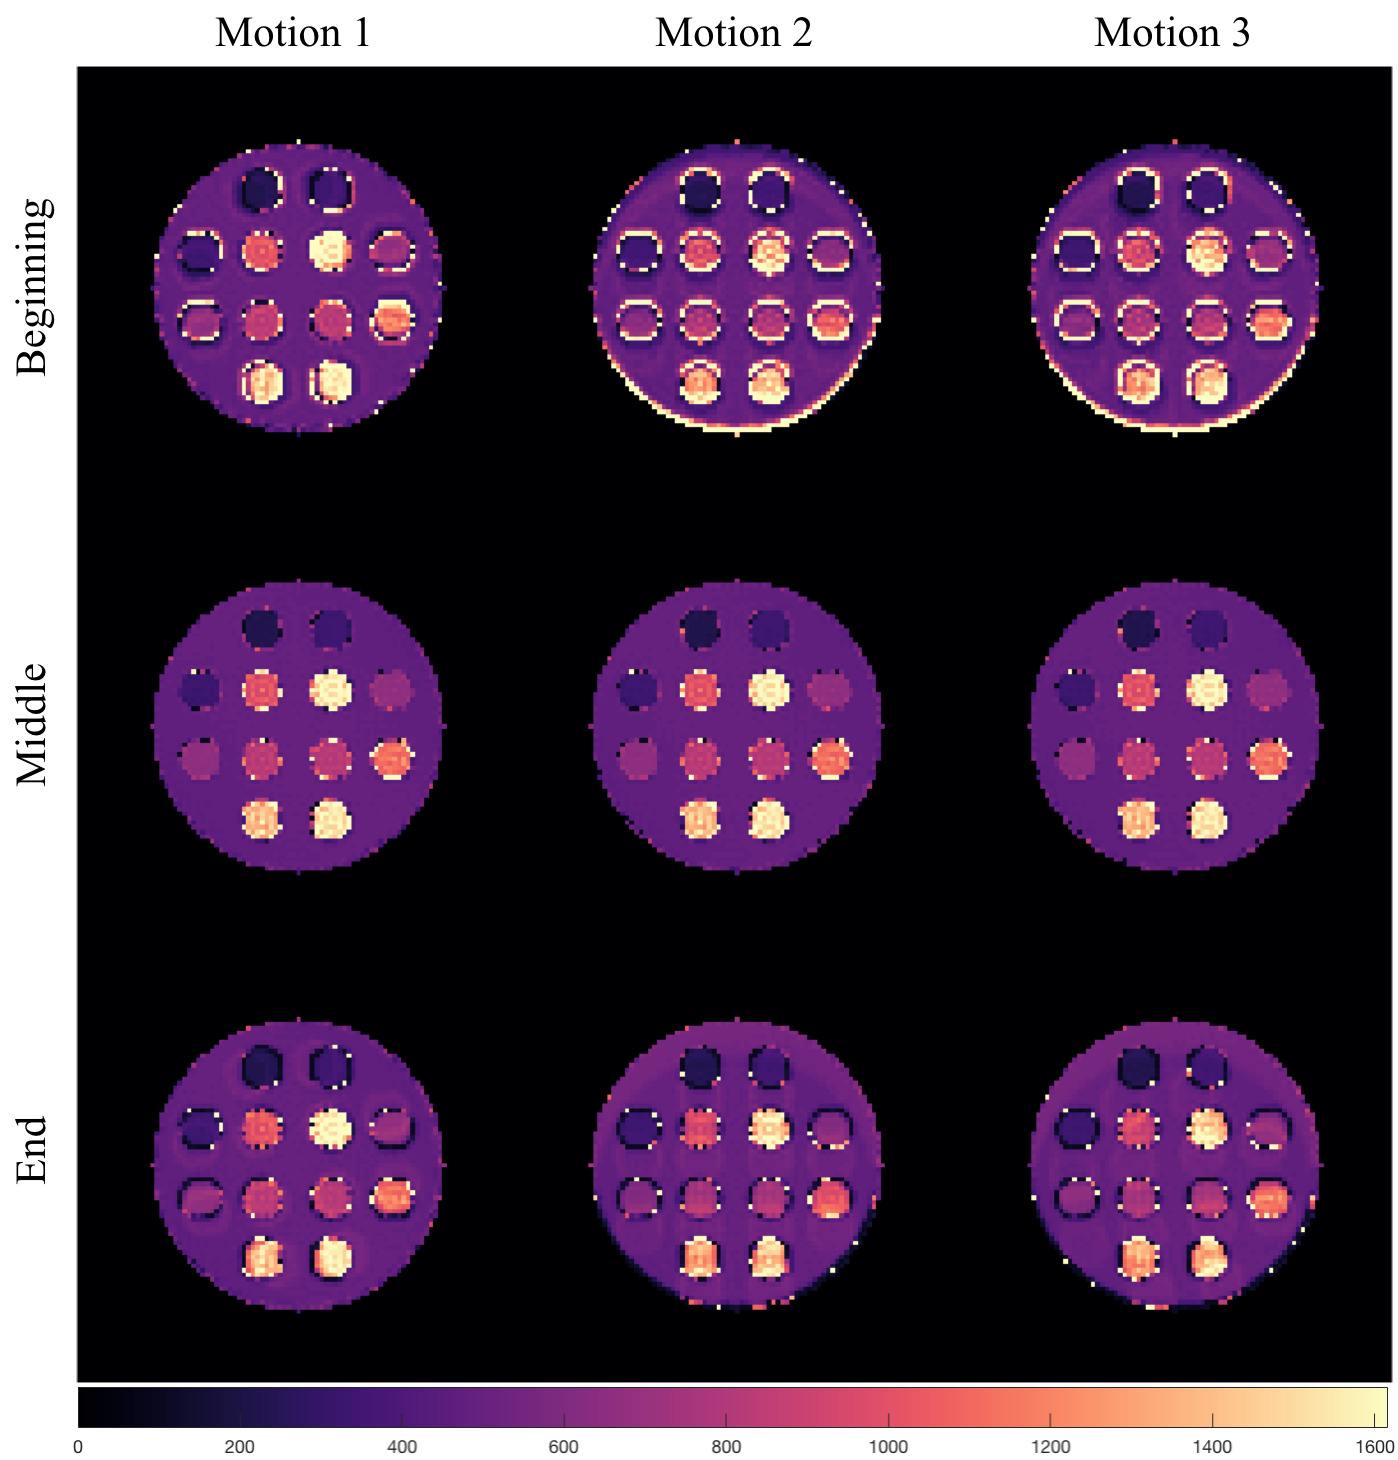
\includegraphics[width=\textwidth]{images/mrf/T1mapsmotion}
        \caption{Motion corrupted $T_1$ maps}
    \end{subfigure}
    
    \begin{subfigure}[b]{.65\textwidth}
        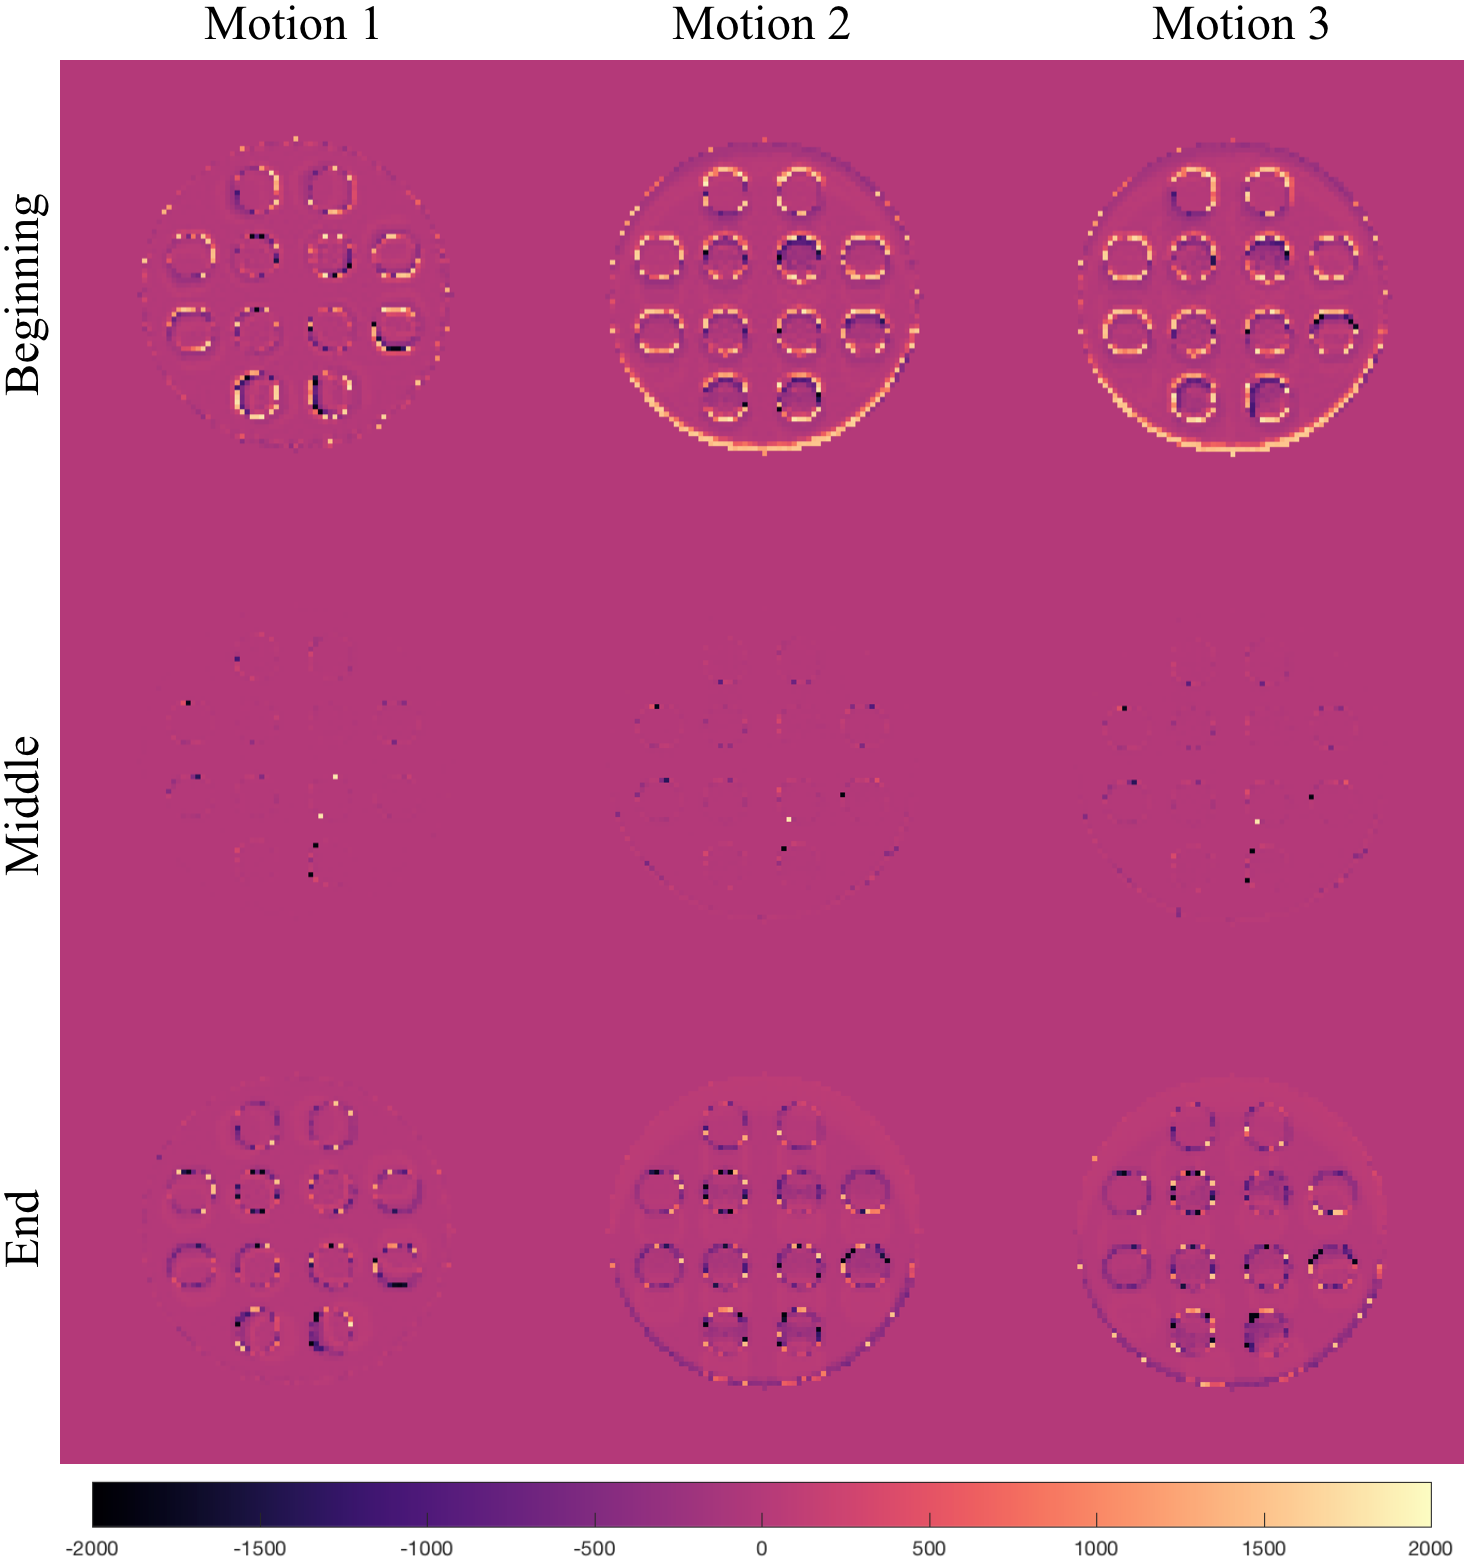
\includegraphics[width=\textwidth]{images/mrf/T1SimuMinusT1Real}
        \caption{Difference between $T_1^{motion \, \, corrupted}$ and $T_1^{motion \, \, free}$}
    \end{subfigure}
    
    \caption{Motion corrupted $T_1$ quantitative maps for all 9 types of motion traces. First column corresponds to the \textit{motion 1} trace (continuous rotation about the z-axis), the second column corresponds to the \textit{motion 2} trace (continuous translation along the y-axis) and the third column corresponds to the \textit{motion 3} trace (continuous rotation about the z-axis and continuous translation along the y-axis). Different lines correspond to a different onset of motion.}
    \label{fig:T1mapsmotion}
\end{figure}
% \begin{figure}[ht]
%     \centering
%     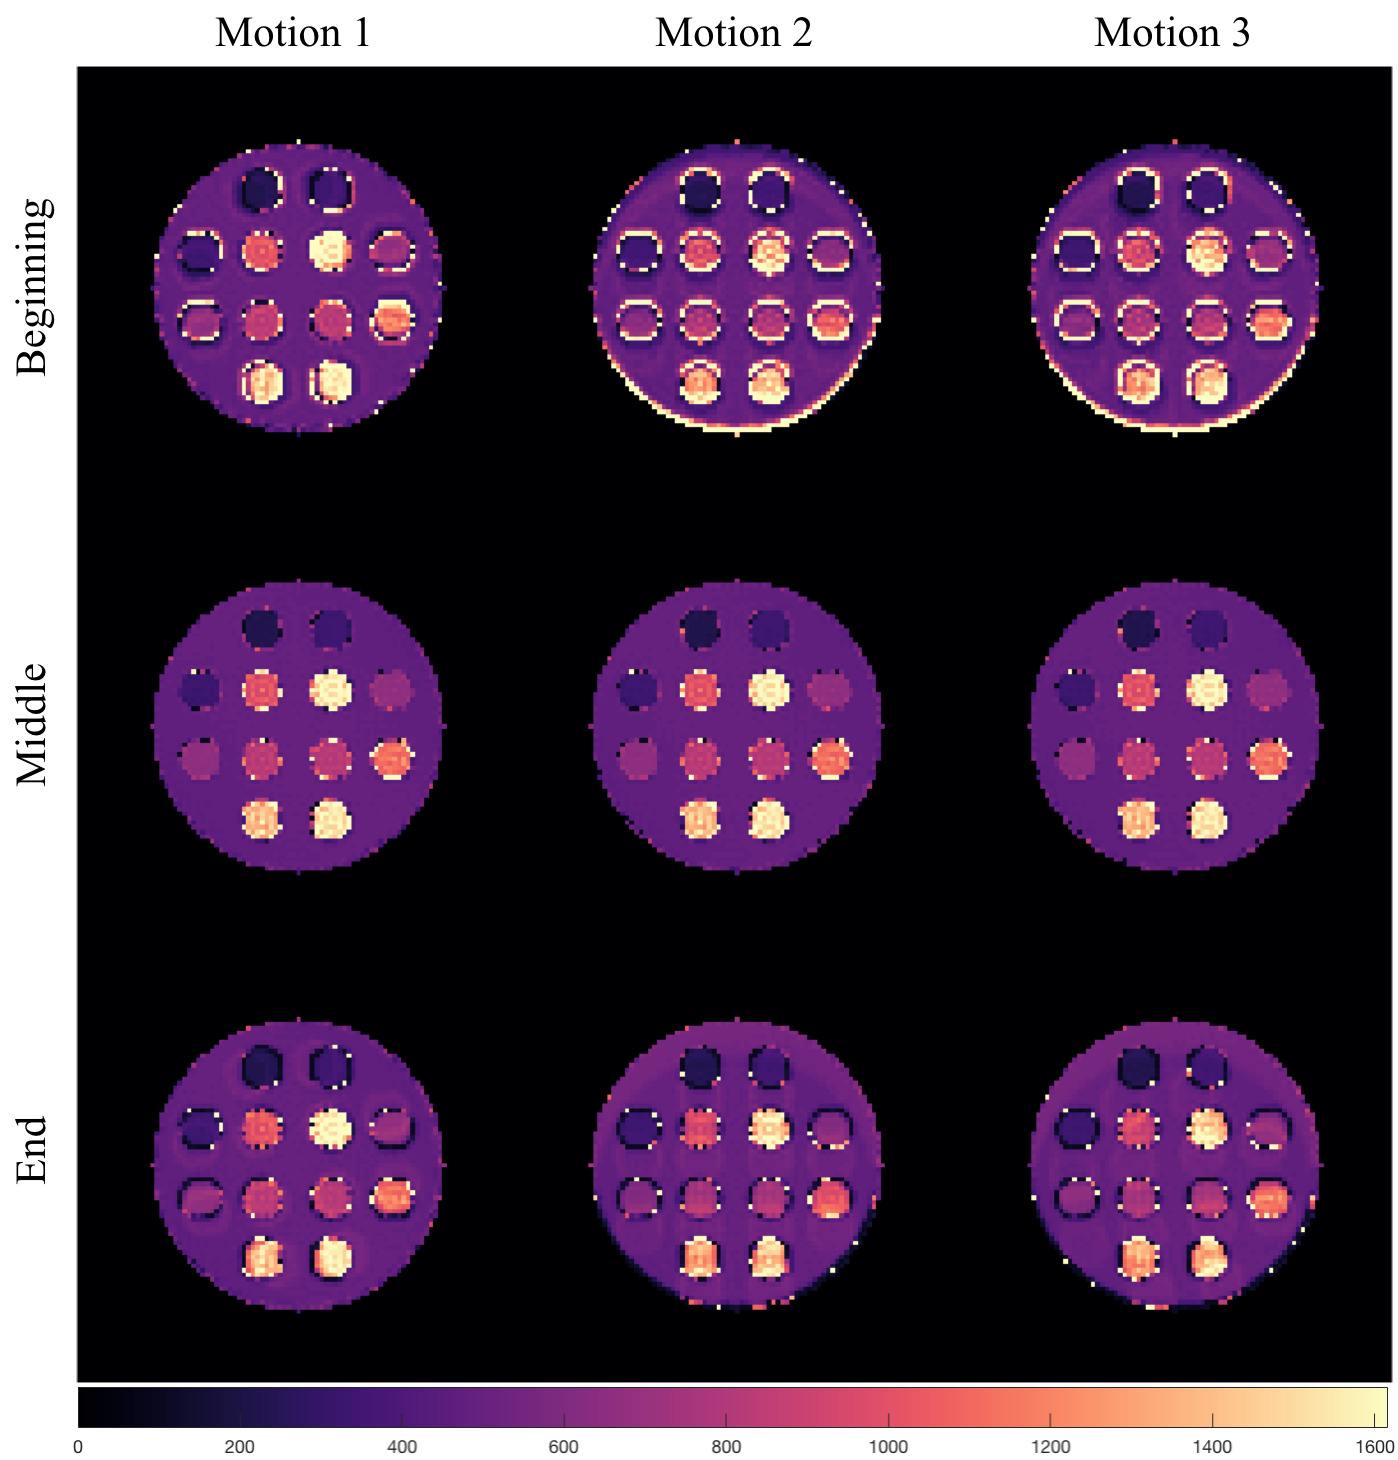
\includegraphics[width=0.85\textwidth]{images/mrf/T1mapsmotion}
%     \caption{Motion corrupted $T_1$ quantitative maps for all 9 types of motion traces. First column corresponds to the \textit{motion 1} trace (continuous rotation about the z-axis), the second column corresponds to the \textit{motion 2} trace (continuous translation along the y-axis) and the third column corresponds to the \textit{motion 3} trace (continuous rotation about the z-axis and continuous translation along the y-axis). Different lines correspond to a different onset of motion. }
%     \label{fig:T1mapsmotion}
% \end{figure}

% T2 maps motion
\begin{figure}[ht]
    \centering
    \begin{subfigure}[b]{.65\textwidth}
        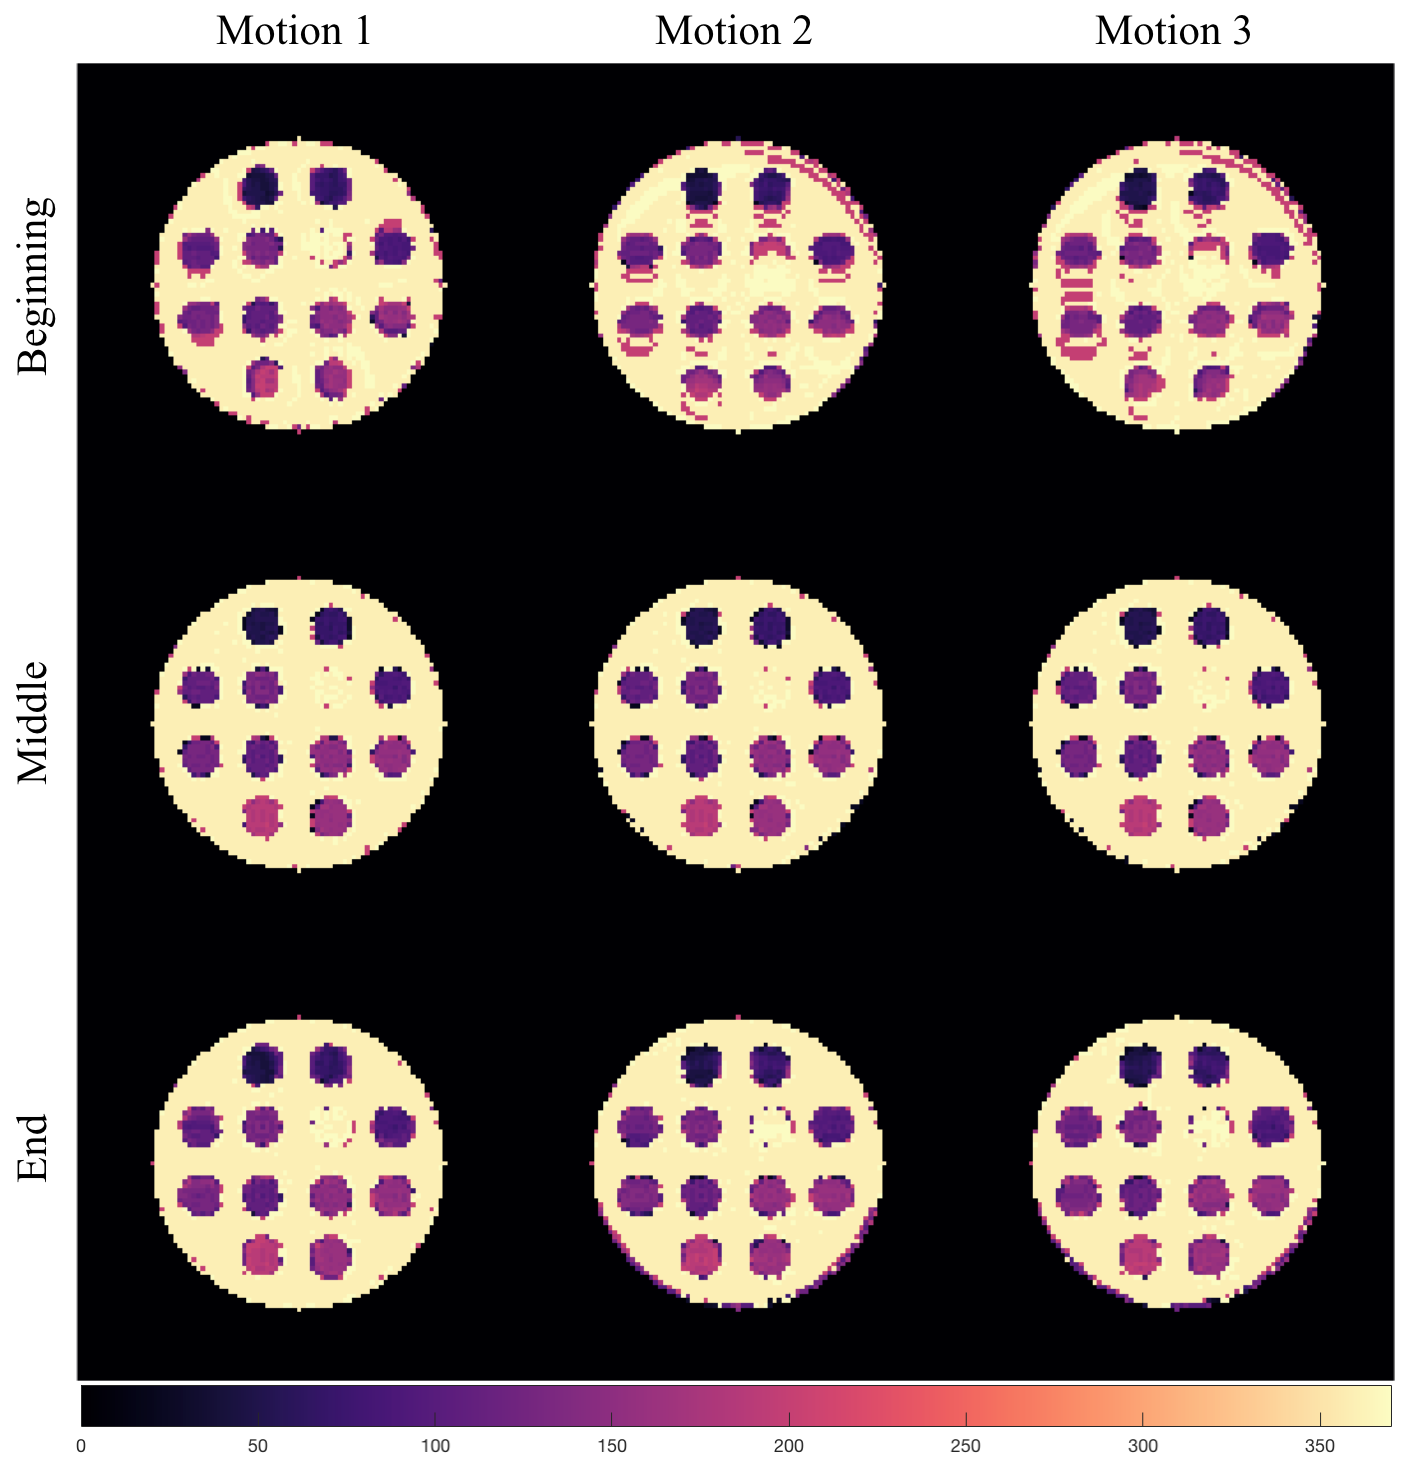
\includegraphics[width=\textwidth]{images/mrf/T2mapsmotion}
        \caption{Motion corrupted $T_2$ maps}
    \end{subfigure}
    
    \begin{subfigure}[b]{.65\textwidth}
        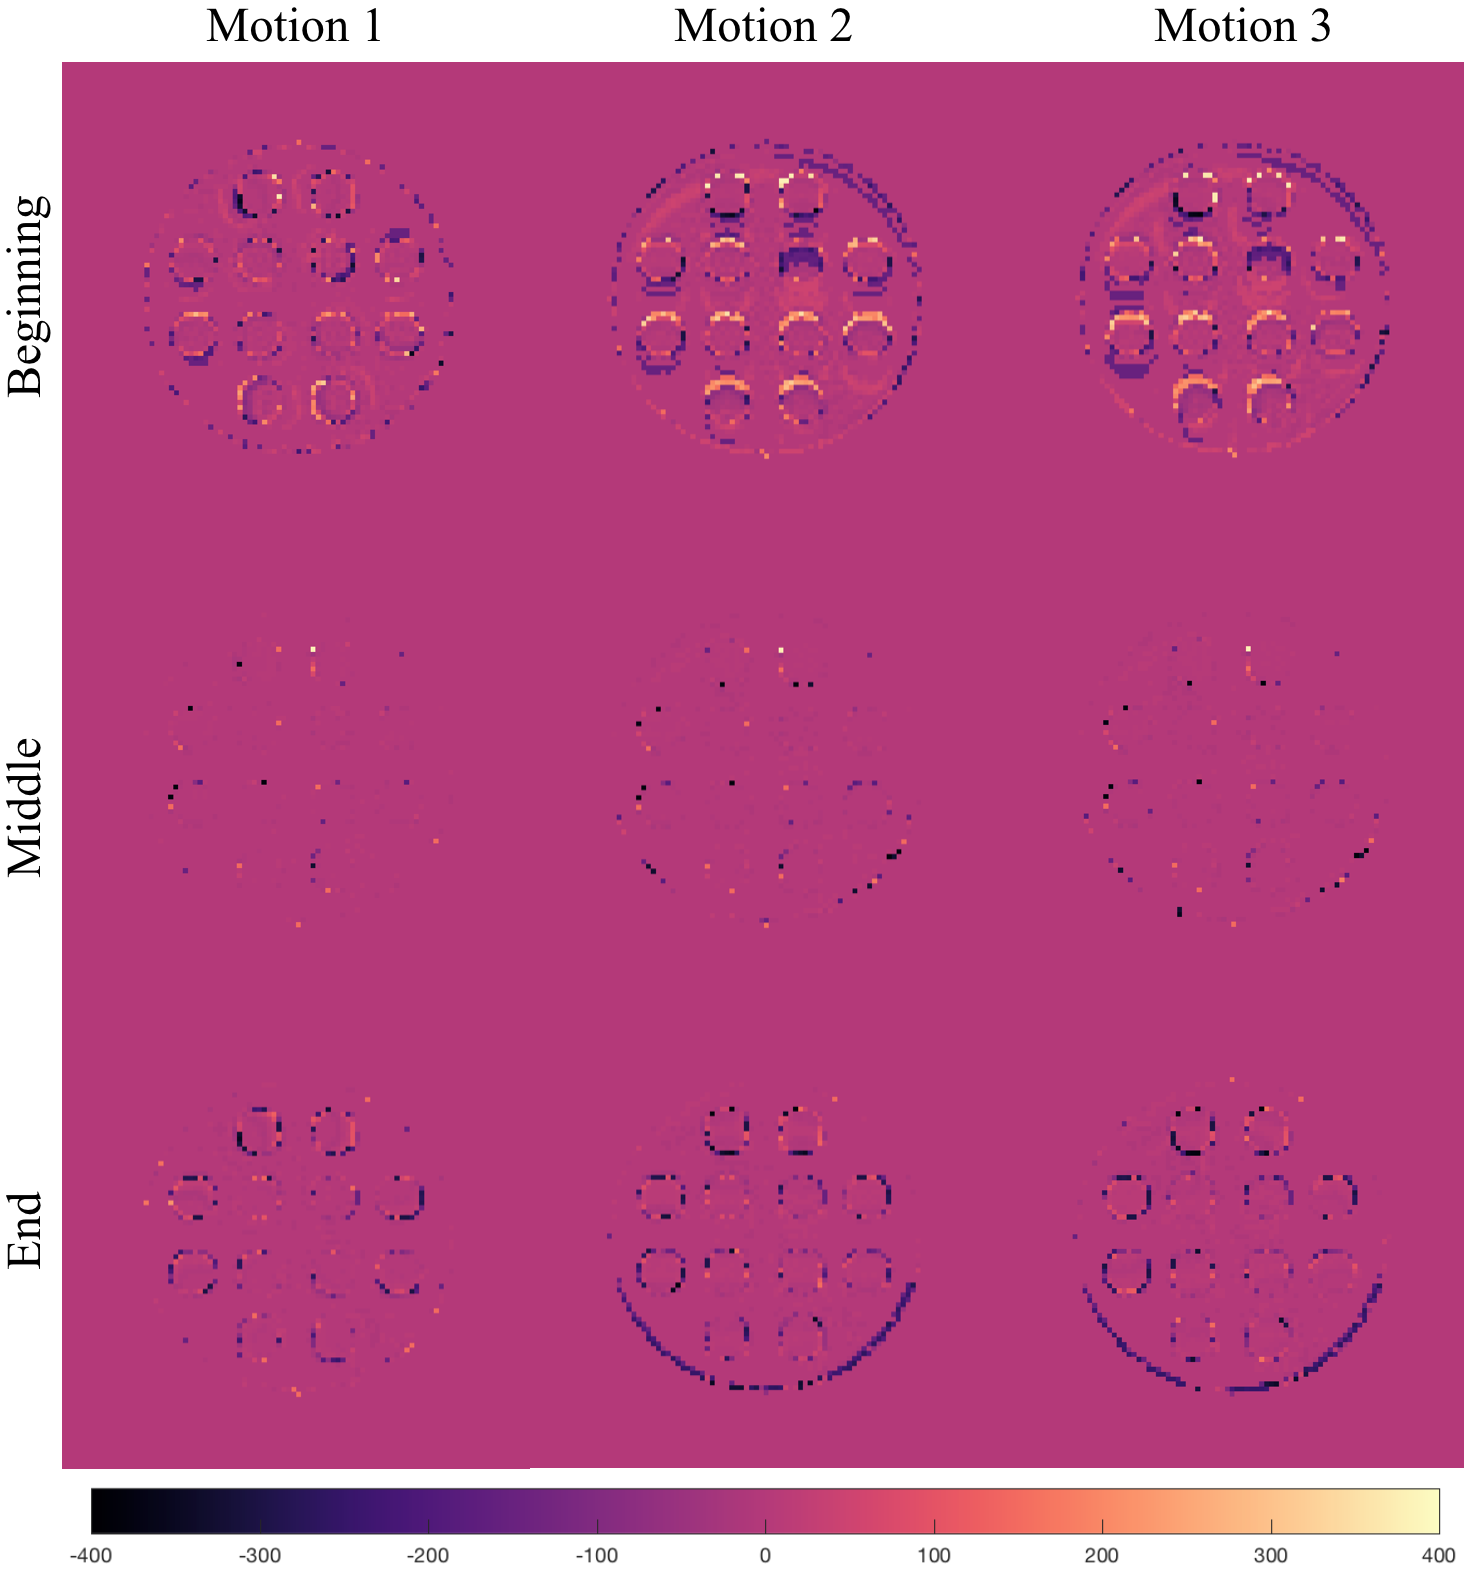
\includegraphics[width=\textwidth]{images/mrf/T2SimuMinusT2Real}
        \caption{Difference between $T_2^{motion \, \, corrupted}$ and $T_2^{motion \, \, free}$}
    \end{subfigure}
    
    \caption{Motion corrupted $T_2$ quantitative maps for all 9 types of motion traces. First column corresponds to the \textit{motion 1} trace (continuous rotation about the z-axis), the second column corresponds to the \textit{motion 2} trace (continuous translation along the y-axis) and the third column corresponds to the \textit{motion 3} trace (continuous rotation about the z-axis and continuous translation along the y-axis). Different lines correspond to a different onset of motion.}
    \label{fig:T2mapsmotion}
\end{figure}
% \begin{figure}[ht]
%     \centering
%     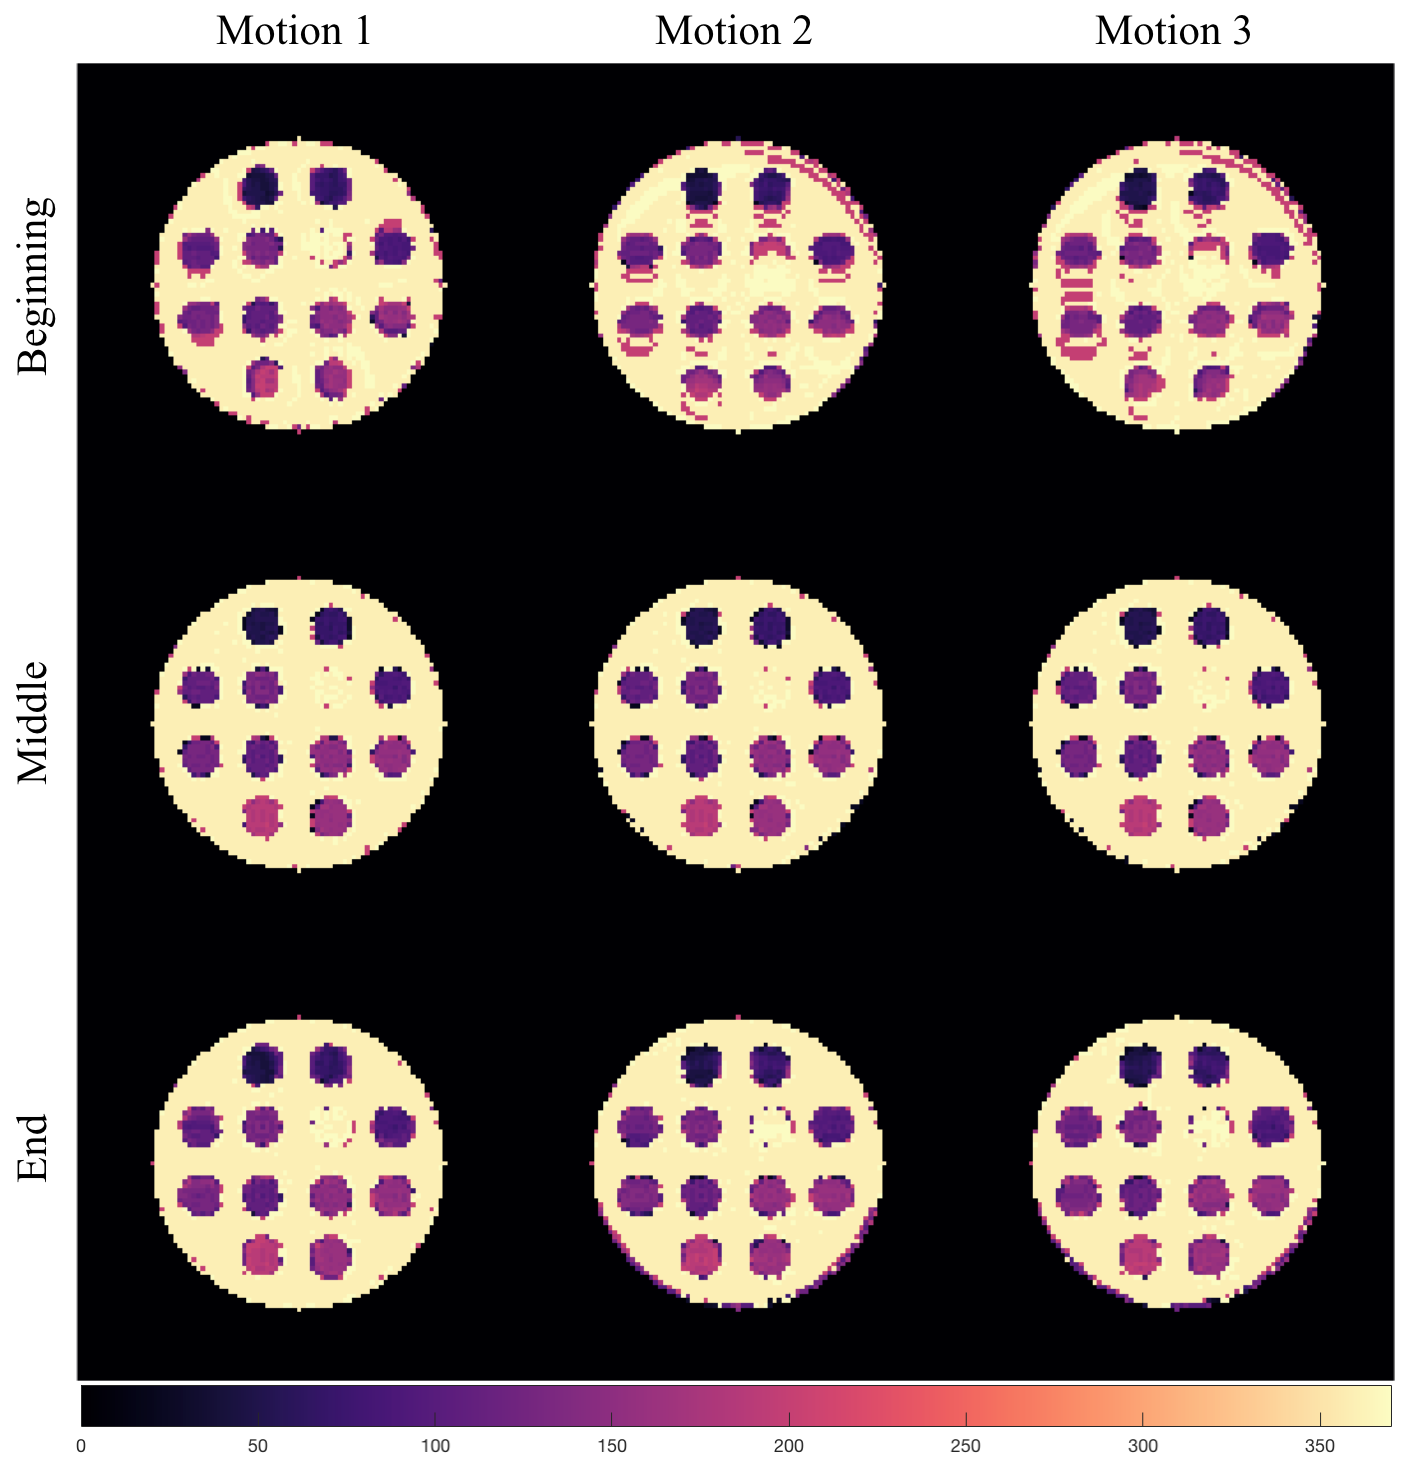
\includegraphics[width=0.85\textwidth]{images/mrf/T2mapsmotion}
%     \caption{Motion corrupted $T_2$ quantitative maps for all 9 types of motion traces. First column corresponds to the \textit{motion 1} trace (continuous rotation about the z-axis), the second column corresponds to the \textit{motion 2} trace (continuous translation along the y-axis) and the third column corresponds to the \textit{motion 3} trace (continuous rotation about the z-axis and continuous translation along the y-axis). Different lines correspond to a different onset of motion. }
%     \label{fig:T2mapsmotion}
% \end{figure}
% % % END images here:

% The other regions of interest are further from the centre and will all be affected by motion.
% More specifically, $T_2$ values are most affected when motion is happening at the beginning of the scan, regardless of the type of motion, and least affected when motion is happening in the middle or at the end of the scan.
% One potential reason for this is that the fingerprints are least discriminative in the middle of the scan for different $T_2$ values (see Figure~\ref{fig:mrfDictionaries} (b)).
% Similarly, $T_1$ values are also affected by motion happening at the beginning of the scan.
% In this case, small $T_1$ values (tubes 1 and 3) are always overestimated regardless of the type of motion, while higher $T_1$ values (tubes 5 and 12) are underestimated when translation is occurring.
% Moreover, motion occurring in the middle of the scan leads to overestimated high $T_1$ values (tubes 5 and 12), but does not affect lower $T_1$ values (tubes 1 and 3).

% \hfill

To further understand the impact of motion on the simulated maps, I decided to have a closer look at individual signals. 
Figure~\ref{fig:motion1ROIsignals} shows together the motion free signal (black dashed) and its dictionary match (green dashed), together with the motion corrupted signal (red) and its corresponding dictionary match (blue dashed), for continuous rotation with different onsets.
The plots show that the motion corrupted signal is matched to a different fingerprint than the motion free signal when the onset is at the beginning or at the end of the scan.
When motion is happening in the middle of the scan, the matching algorithm still finds the ground truth values.

% Motion 1 signals
\begin{figure}[ht]
    \centering
    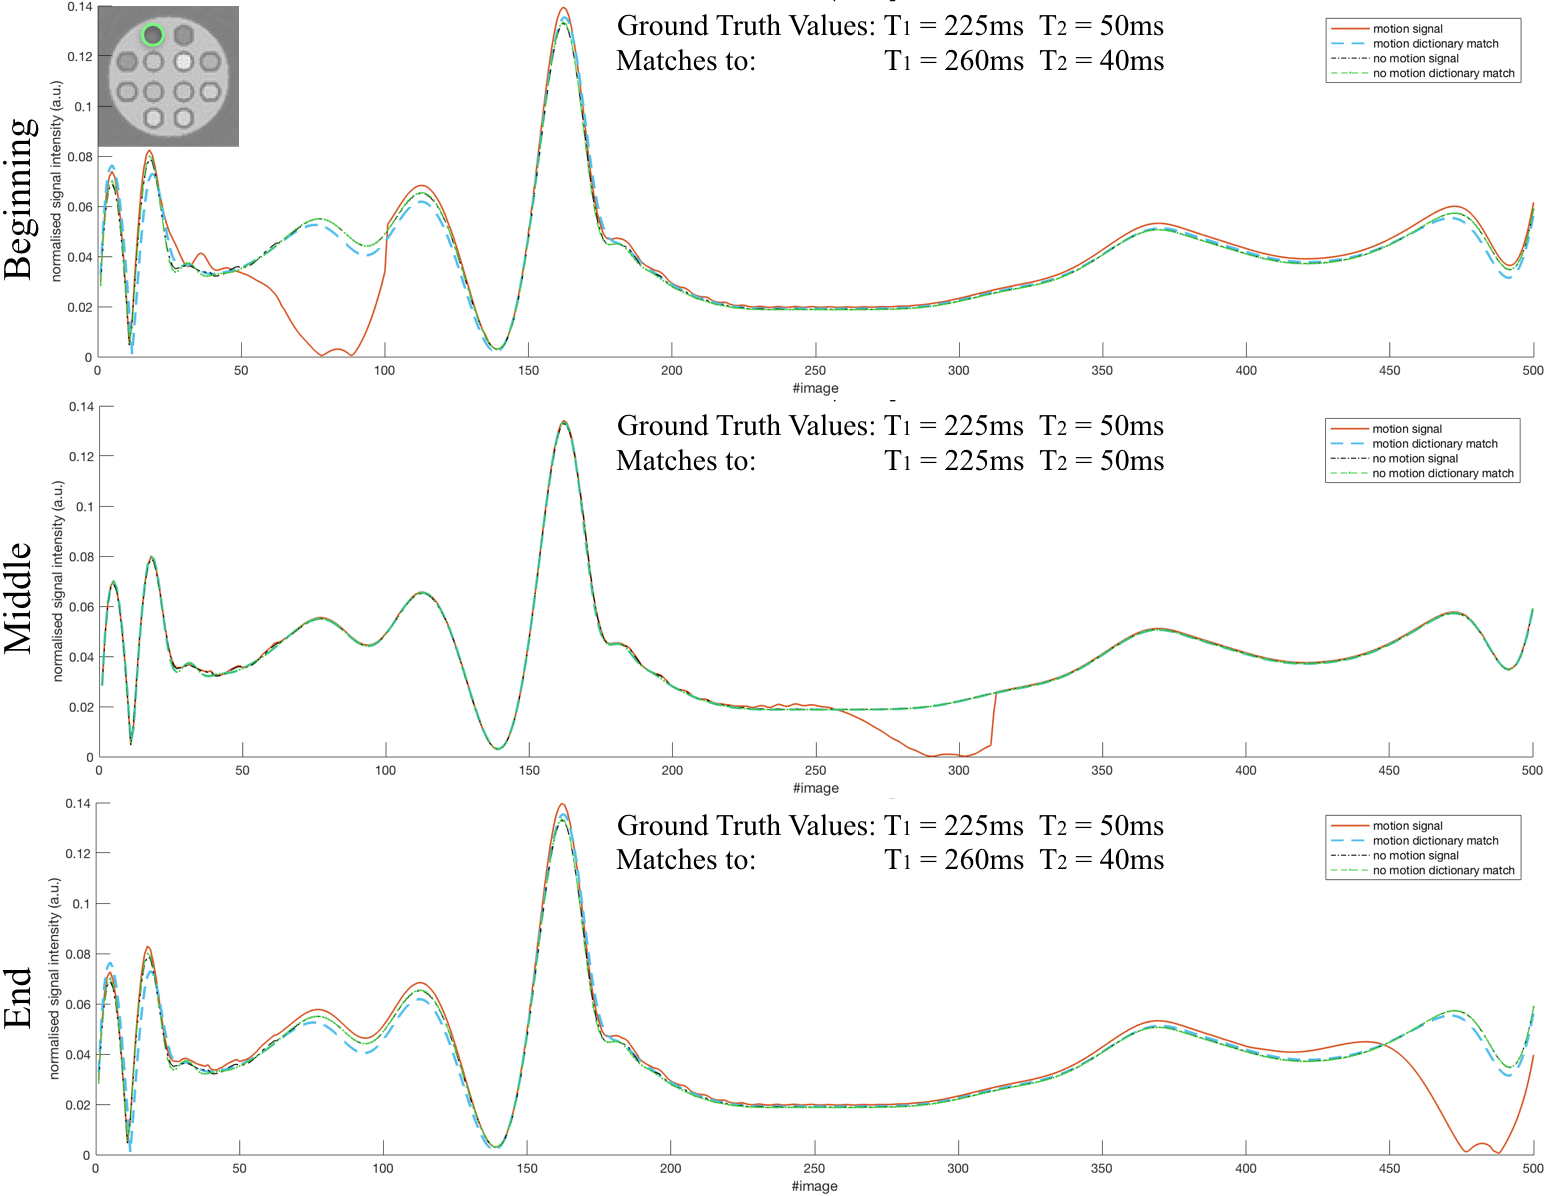
\includegraphics[width=0.95\textwidth]{images/mrf/motion1ROIsignals}
    \caption{Comparison between the motion free dictionary match and the motion corrupted dictionary match for different onsets of motion. Type of motion shown here is \textit{motion 1}.}
    \label{fig:motion1ROIsignals}
\end{figure}

\hfill

Figure~\ref{fig:motion2ROIsignals} shows a similar trend for the second type of motion.
However, in this plot a different voxel was chosen which corresponds to a higher $T_1$ value.
Here, all three types of onset affect the reconstructed values.
The least affected signal is, again, the one corresponding to motion happening in the middle of the scan, with the transverse relaxation time $T_2$ matched to the ground truth value of $160ms$.
As stated before, we speculate that the $T_2$ values are least affected here because the dictionary fingerprints are very similar to each other during the onset of motion (see  Figure~\ref{fig:problematicfingerprints}).

% Motion 2 signals
\begin{figure}[ht]
    \centering
    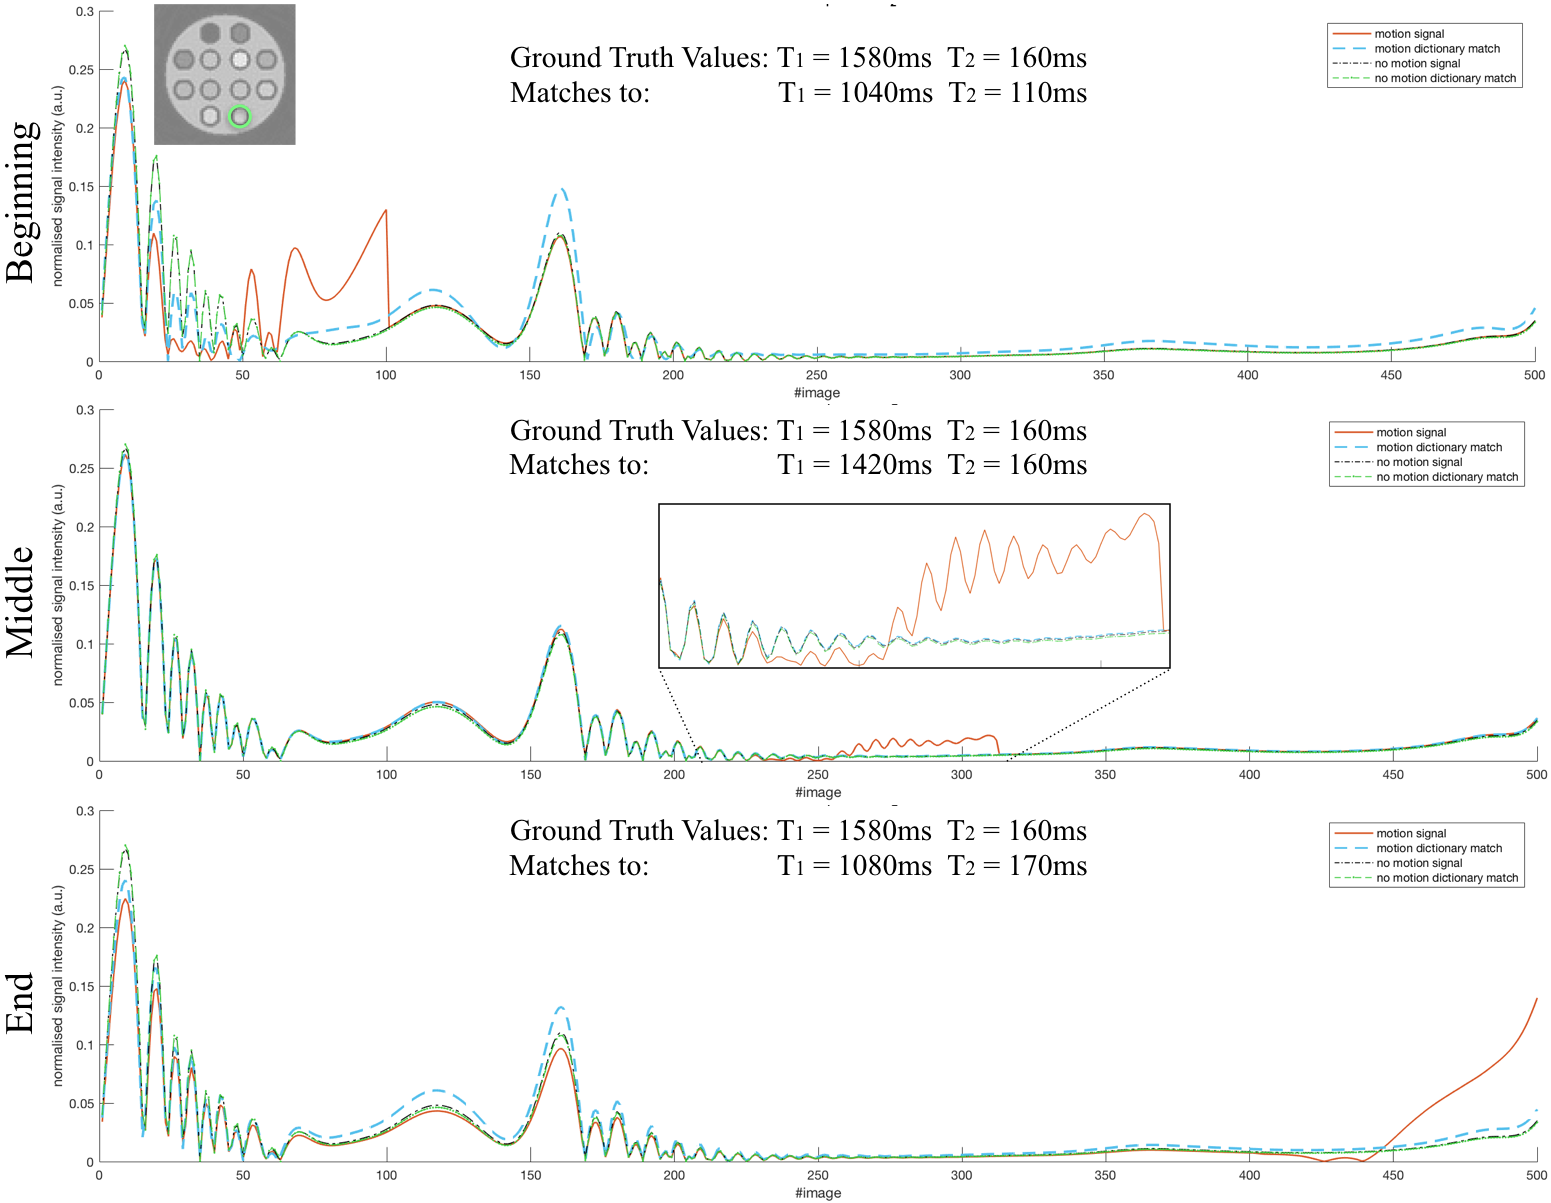
\includegraphics[width=0.95\textwidth]{images/mrf/motion2ROIsignals}
    \caption{Comparison between the motion free dictionary match and the motion corrupted dictionary match for different onsets of motion. Type of motion shown here is \textit{motion 2}.}
    \label{fig:motion2ROIsignals}
\end{figure}


% % % % % % % % % % % % % % % % 
\section{Conclusions}\label{chapterlabel3sec4}

In this work I showed a proof-of-concept image space simulation pipeline of a magnetic resonance fingerprinting experiment.
The proposed method uses a physics-based approach to the MR acquisition process in order to simulate the MRI datasets.
Moreover, I investigated the impact of in-plane rigid motion applied at various time points during the scan on the final quantitative maps.
In this approach, the motion artifacts were introduced during the acquisition of the signal which made these simulations more realistic than other approaches where datasets were corrupted by applying geometric transformations in image space (see Section \ref{chapterlabel2sec2}).

\hfill

This investigation shows that MRF may not be as robust to motion as previously suggested and that the severity of its impact is strongly dependent on the type of motion, its onset and the dictionary construction.
However, motion is not necessarily restricted to in-plane movements.
Through-plane motion can happen during a real scan and it could have a different impact on the $T_1$ and $T_2$ maps.
Moreover, a real scan cannot use a fully sampled spiral readout due to hardware constraints, but uses a variable density spiral readout with multiple interleaves.
This is a limitation of my current approach, but I aim to cover it in future work.


%%%%%%%%%%%%%%%%%%%%%%%%%%%%%%
%% CHAPTER 4 - Conclusions and Future Work
%%%%%%%%%%%%%%%%%%%%%%%%%%%%%%
\chapter{Conclusions and future directions}
\label{chapterlabel4}
\epigraph{``Good judgement comes from experience. Experience comes from bad judgement."}{--- \textup{Unknown}}

%In this work we demonstrated that there is a need to have a realistic MRI simulation framework to accurately and precisely investigate the nature of commonly occurring MRI artefacts.
%Although others before us have succeeded in developing MR simulators capable of constructing MRI datasets (see Chapter \ref{chapterlabel2secMRISIMULATORS}), there are limitations that need to be overcome in order to push the research towards more advanced sequences such as magnetic resonance fingerprinting (see Chapter \ref{chapterlabel2sec2}).

The main aim of this PhD project is to develop a magnetic resonance imaging simulation framework capable of simulating advanced \ac{mri} sequences and to demonstrate its application on a novel quantitative \ac{mri} protocol known as \ac{mrf}.

% % % Contributions to date
% % % % % % % % % % % % % % % % 
\section{Contributions to Date}\label{chapterlabel4sec1}

Towards this aim I have made the following contributions:

\begin{enumerate}

	\item Carried out a study of the relevant background theory for understanding Magnetic Resonance Imaging (Appendix \ref{appendixlabelBackgroundMRI}) and Magnetic Resonance Fingerprinting (Appendix \ref{appendixlabelBackgroundMRF}).
	
	\item Carried out a comprehensive literature review consisting of the current state-of-the-art in both Magnetic Resonance Imaging (Chapter \ref{chapterlabel2sec1} and Chapter \ref{chapterlabel2secMRISIMULATORS}) and Magnetic Resonance Fingerprinting simulation systems (Chapter \ref{chapterlabel2sec2}).
	%Additionally, as a result of this study, we provide a generalised software framework for an ideal MRI simulator that can serve as a guideline for the MRI simulation community worldwide (Chapter \ref{chapterlabel4sec2}).
	
	\item Implemented a proof-of-concept simulation framework for a Magnetic Resonance Fingerprinting experiment in an open-source simulator called JEMRIS \cite{Stocker2010}.
	Our choice of simulator environment was based on the availability of a sequence development tool offered with the simulator.
	Our implementation involved the development of the original MRF sequence \cite{Ma2013}.
	Additionally, we have investigated the impact of in-plane motion beginning at various time points during the scan.
	This framework and our results were detailed in Chapter \ref{chapterlabel3}.
	
\end{enumerate}

% % % % Work Plan
% % % % % % % % % % % % % % % % 
\section{Work Plan}\label{chapterlabel4sec2}

These contributions demonstrate the potential value of a simulation system for advanced \ac{mri} sequences. 
Future work will focus on five areas:

%The PhD contributions so far demonstrate the value for an MRI simulation frame-work capable of producing realistic MRI datasets of advanced sequences in anaccurate and rapid manner. Future work will therefore include:

\begin{enumerate}
    % % % 
    %\item \textit{Write an MRI simulators review paper.}
    \item \textit{\textbf{Write an \ac{mri} simulators review paper} (first entry in Figure~\ref{fig:ganttChart})} \\
    So far, I have investigated the current state-of-the art in \ac{mri} simulation systems and experimented with 2 of the most popular and active \ac{mri} simulators today.
    It is my plan for the future work to focus on fleshing out the literature review of this thesis into a review paper.
    
    % % % 
	\item \textit{\textbf{Continue with motion-corrupted \ac{mrf} experiments} (second entry in Figure~\ref{fig:ganttChart})} \\
	So far, I have investigated how in-plane motion corrupts the \ac{mrf} quantitative maps.
	In the future, I aim to investigate through-plane motion and a combination of both in-plane and through-plane motion for the original \ac{mrf} implementation by Ma et al. \cite{Ma2013}.
	
	% % % 
	\item \textit{\textbf{Develop an open-source MRI simulator that will allow for the simulation of advanced MRI sequences} (third entry in Figure~\ref{fig:ganttChart})} \\
	
	So far, I have implemented a proof-of-concept simulation framework for an \ac{mrf}-\ac{bssfp} experiment in an open-source simulator called JEMRIS \cite{Stocker2010}.
	However, the newest implementation of an \ac{mrf} sequence relies on a \ac{fisp} type acquisition protocol for which a high number of isochromats is required in order to achieve realistic results \cite{Hennig1991}.
	With the current JEMRIS implementation, this would require an unfeasibly long time to simulate.
	The reason for this is:
	
	\begin{itemize}
	    
	    \item I have calculated that a JEMRIS numerical simulation of a single voxel \ac{fisp} protocol that achieves the same results as the \ac{epg} implementation shown in Chapter \ref{method:fispdictionary} would require around 5000 isochromats. \\
	    
	    In my current implementation the input object consists of 4145 isochromats in total and requires a total time of 12 hours to run.
	    This means that in order to achieve accurate results I would need to discretise the input object to contain approximately 21 million isochromats.
	    This would bring the current simulation time to almost a year.
	    
	\end{itemize}
	
    % 	On the other hand, my own MATLAB simulations of a single voxel \ac{fisp} experiment show that I can achieve the same accuracy as an \ac{epg} implementation with approximately 200 isochromats.
	For this reason, it is my plan for future work to develop an open-source MRI simulator based on \ac{gpu} parallelisation and the newest programming standards offered by CUDA 9.x.
	The reasons for choosing \ac{gpu} parallelisation are:
	
	\begin{itemize}
	    
	    \item Xanthis et al. \cite{Xanthis2014} showed that their \ac{gpu}-based \ac{mri} simulation system can achieve a speedup of $31$ to $115$ times compared to OpenMP \ac{cpu} parallelisation.
	    However, their simulator is neither open-source, nor freely available to be downloaded and used.
	    
	    \item In their experiment they simulated a simple gradient echo sequence using an input object of $15 \times 15 \times 15cm$ consisting of $1, 350, 000$ isochromats (or, $400$ isochromats in every $cm^3$).
	    Their simulation took approximately $4.8$ minutes.
	    
	    \item My own MATLAB simulations of a single voxel \ac{fisp} experiment show that I can achieve the same accuracy as an \ac{epg} implementation with approximately 200 isochromats.
	    This means that I could bring down the simulation time to 40 hours by using the same experiment design as Xanthis et al. \cite{Xanthis2014}, but with $200$ isochromats in every $mm^3$ of a $15 \times 15 \times 15cm$ object and considering a linear increase in the simulation time.
	    Their implementation, however, is on a single board \ac{gpu} personal computer and it uses an older version of the CUDA \ac{api}.
	    I am to use the newest CUDA standards and more recent GPU hardware which could further improve the run time.
	    
	\end{itemize}
	
	Implementing the open-source \ac{gpu}-based MRI simulator will consists of the following steps:
	\begin{enumerate}
	    
	    \item One voxel experiments:
	    \begin{itemize}
	        \item Develop a simple \ac{bssfp} experiment (single readout, multiple repetition periods) and compare it against my current MATLAB implementation.
	        
	        \item Develop a simple \ac{fisp} experiment (single readout, multiple repetition periods) compared it against my current MATLAB implementation.
	        
	        \item Experiment with different numbers of isochromats and find the critical number of spins required.
	    \end{itemize}
	    
	    \item Multiple voxel experiments:
	    \begin{itemize}
	        \item Develop a simple \ac{bssfp} experiment (EPI readout, one repetition period) and compare it against my current JEMRIS implementation.
	        
	        \item Develop a simple \ac{fisp} experiment (EPI readout, one repetition period) and compare it against my current JEMRIS implementation.
	        
	    \end{itemize}
	    
	    \item Develop the full \ac{mrf}-\ac{fisp} sequence.
	    
	\end{enumerate}	
	
	The general framework for my proposed simulation system is presented in the next section.
	In the remaining time of my PhD the focus will be on the development of a \ac{gpu}-based Bloch equation solver.
	
    % 	However, in order to mimic a continuous distribution of spins throughout an object voxel, a high number of isochromats is required to generate a smooth image intensity \cite{Shkarin1997}.
    % 	Moreover, newer \ac{mrf} implementations rely on an imaging sequence called fast imaging with steady state precession (\ac{fisp}, see Appendix \ref{MRIFISP}) which requires an even denser collection of spins to be accurate.
	
	\item \textit{\textbf{Validate the implementation} (fourth entry in Figure~\ref{fig:ganttChart})}
	So far, the simulation system has not been validated.
	This is because the real \ac{mrf} datasets that I have are for the \ac{mrf}-\ac{fisp} implementation.
	For this reason, I aim to demonstrate the applicability of my new simulator by validating it against real \ac{mrf}-\ac{fisp} datasets.
	
	\item \textit{\textbf{Simulate the impact of motion on the \ac{mrf}-\ac{fisp} sequence} (fifth entry in Figure~\ref{fig:ganttChart})}
	After validation, I will be in a great place to investigate the impact of motion on the \ac{mrf}-\ac{fisp} sequence.
	For this, I aim to look at in-plane, through-plane and a combination of both in-plane and through-plane motion for the newly developed simulation system.
	
\end{enumerate}

\begin{figure}[ht]
    \centering
    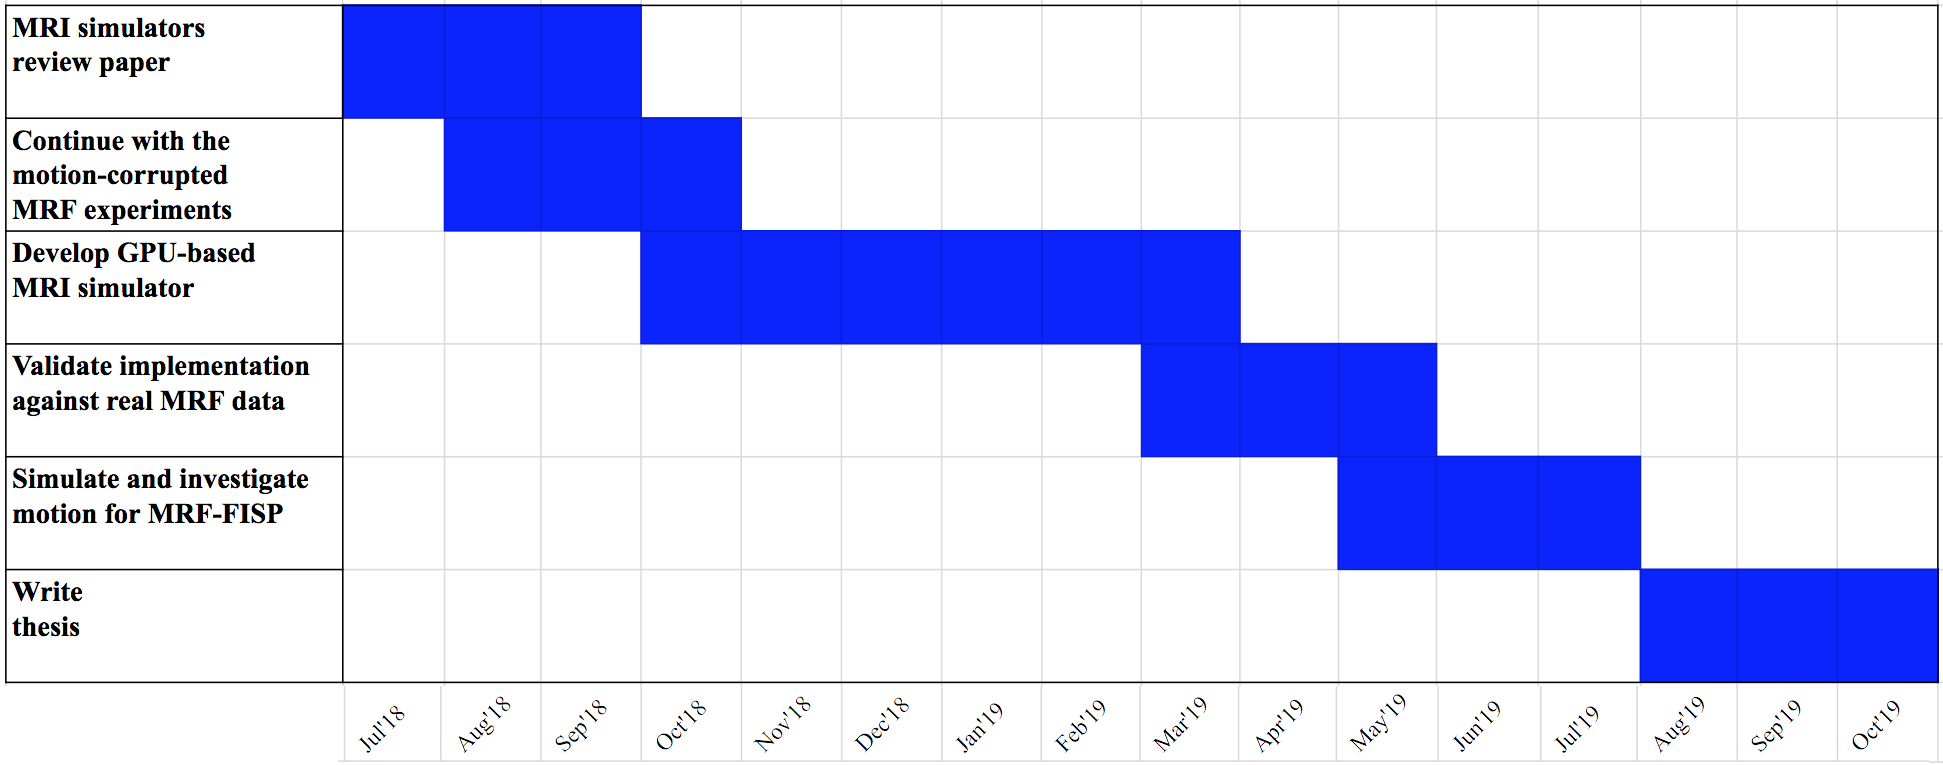
\includegraphics[width=1\textwidth, keepaspectratio]{images/mri/ganttChart}
    \caption{Gantt chart demonstrating how I will spend the remaining time in my PhD}
    \label{fig:ganttChart}
\end{figure}


% % % % Generalised API
% % % % % % % % % % % % % % % % 
\section{Proposed Framework for an Ideal MRI Simulation System}
\label{chapterlabel4sec3}

This section focuses on introducing a generalised framework for an ideal \ac{mri} simulator to serve as a guideline for the \ac{mri} simulation community.
It is my belief that the proposed structure will aid in overcoming major limitations found throughout available simulators today and will also set the stage for my future work in my PhD project.
%Moreover, this framework can be used by the \ac{mri} simulation community as a unifying guideline.
This section gives an overview of the framework's components, while focusing on the simulation computational kernel.

\hfill

\large \textbf{Overview of framework} \normalsize

The proposed framework is summarised in Figure~\ref{fig:globalFramework} and it consists of the following 6 components:

\hfill

\textbf{Solver.} At the heart of this framework is the \textbf{Bloch Equation Solver}, which independently solves the Bloch equation for each spin in the input object.
The \textbf{solver} is a highly parallelizable component of the framework which can run either on a \ac{gpu} architecture.
The solver requires the following inputs:
\begin{itemize}
    \item \textbf{Sample Information}, such as:
    \textit{tissue specific parameters} (the nature of the nuclei, proton density, relaxation times and chemical shift), 
    \textit{geometry of the sample} (spin coordinates, resolution, total number of spins), and 
    \textit{motion trace} (translation and rotation values for each time point of the sequence).
    
    \item \textbf{Pulse Sequence Information}, such as:
    % \textit{Sequence Specific timings} (number of pulses in a multi-pulse sequence, repetition times and echo times),
    \textit{Radiofrequency Pulses} (amplitude and phase, duration, shape and timing), 
    \textit{Gradients} (shape, duration, timing) and
    \textit{Readout} (timing of each readout point).
    
    \item \textbf{Scanner Hardware Information}, such as:
    \textit{Main Magnet} (field strength, inhomogeneities in the main magnetic field),
    \textit{Gradient Limits} (maximum amplitude, slew rate) and
    \textit{Receiving/Transmitting Coils} (inhomogeneities in the coils, spatial sensitivity maps). 
\end{itemize}

\hfill

\textbf{Controllers.} The inputs described above are ubiquitous to any type of \ac{mri} simulation protocol.
However, my \textbf{Bloch equation solver} expects them in a certain format.
To overcome this limitation and to make my framework easily extensible, customisable and user friendly, I propose the existence of \textbf{Controllers}.
These are software wrappers which will translate user specific inputs into solver inputs.
With their help, the user can easily decide the complexity of the \ac{mri} simulation by choosing to include or exclude different sample specific, pulse sequence specific or hardware specific parameters.

\hfill

\textbf{Inputs.} The inputs to these controllers come in a variety of forms. 
For the sample object, the user can decide to either use a NIFTI phantom such as the \textit{BrainWeb digital brain phantom} \cite{Kwan1997}, or to create their own parameter maps consisting of the proton density, relaxation times and others.
If any of the required parameters are missing, a message will instruct the user about this error, while optional parameters will be omitted or set to some default values.

\hfill

For the pulse sequence, the user can decide to create their own sequence file consisting of timings ($T_R$, $T_E$), RF pulses ($N_{pulses}$, amplitude and phase), gradients (maximum amplitude, slew rate, shape) and readout timings, or they can use a scanner specific pulse sequence file.
%also choose to experiment with already created classic sequence such as gradient echo, echo planar imaging, etc, and only play with the
Finally, for the hardware configuration inputs, the user can choose to set the field strength ($B_0$) and the hardware limits for their simulation (maximum gradient amplitude, slew rate).
Additionally, for more complex scenarios, users can choose to include multi- transmit or receive coils with separate sensitivity maps or inhomogeneities in the coils.

\hfill

\textbf{GUIs. } Our framework also contains a set of \textbf{graphical user interfaces (GUIs)} which aid the end user in either rapidly prototyping new ideas or creating complex scenarios for \ac{mri} simulations.
Three GUIs are proposed: 
the \textit{Object GUI} for creating the input object and the motion trace,
the \textit{Pulse Sequence GUI} for creating the \ac{mri} pulse sequence and 
the \textit{Hardware Configuration GUI} for the hardware coil configuration.
The outputs from these GUIs become \textbf{inputs} for the software wrappers.

\hfill

\textbf{Reconstruction. } Having all of these in place, the \textbf{Bloch equation solver} will produce a set of signals corresponding to each coil used in the simulation.
These signals will be fed into a \textbf{reconstruction} block which, based on the type of readout used, can perform both Cartesian and non-Cartesian reconstructions.

\hfill

\textbf{Output. } The output of my proposed generalised framework is a set of reconstructed images and, if the option is enabled, the $x,y,z$ components of the magnetisation vector.
We have chosen to include the latter because in my experience with simulating \ac{mri} sequences, I have found it to be very useful to have this extra piece of information available to you.

\clearpage

\large \textbf{GPU-Based Parallel Approach to the Bloch Equation Solver} \normalsize

The computational kernel of the \ac{mri} simulator will initially be based on the solutions of the Bloch equations at every time point in the pulse sequence and for every isochromat in the input object. 
These solutions will provide a temporal evolution of each isochromat's magnetisation vector under the effect of various \ac{rf} pulses, magnetic field gradients and inhomogeneities in the main magnetic field.

\hfill

Mathematically, the vector expression for the Bloch equation is:
\begin{flalign*}
    \frac{\vec{M}}{dt} &= \gamma \big( \vec{M} \times \vec{B}_{eff} \big) - 
    \begin{bmatrix}
    M_x / T_2 \\
    M_y / T_2 \\
    (M_z - \rho M_0) / T_1
    \end{bmatrix}
\end{flalign*}
where
\begin{flalign*}
    \vec{B}_{eff}(\vec{r},t) &= (xG_x(t) + yG_y(t)+ zG_z(t))\hat{z} + \Delta B (\vec{r}, t) \hat{z} + \vec{B}_{1x}(\vec{r},t) + \vec{B}_{1y}(\vec{r},t) 
\end{flalign*}
is the effective magnetic field experienced by the isochromat on position $\vec{r}$ and at time t;
$G_x, G_y $ and $G_z $ are the imaging gradients,
$\vec{B}_1$ is the applied RF pulse and 
$\Delta B$ accounts for off-resonance effects.

\hfill

The evolution of the magnetisation vector will be calculated by the computational kernel for every time-step $\Delta t$ in the pulse sequence using scaling and rotation matrices:
\begin{flalign*}
    \vec{M} (\vec{r}, t+\Delta t) &= (1-E_1) \vec{M}(t=0) + D \, \,  R_{eff} \, \,  \vec{M}(\vec{r},t)
\end{flalign*}
where $E_1 = e^{-\Delta t/T_1}$, 
$E_2 = e^{-\Delta t/T_2}$,
$\vec{M}(t=0)$ is the magnetisation vector at the beginning of the sequence, D is the diagonal matrix:
\begin{flalign*}
    D  & = \left[
    \begin{array}{c c c}
          E_2 &     0      &     0 \\
          0      & E_2 &     0 \\
          0      &     0      & E_1
    \end{array}
    \right]
\end{flalign*}
and $R_{eff} = R_{z}(\phi) R_{y}(-\beta) R_{x}(\alpha) R_{y}(\beta) R_{z}(-\phi)$ is the rotation matrix about the axis of the $\vec{B}_{eff}$ field.
Here, the $\vec{B}_{eff}$ field can have any orientation in the 3D space as it is characterised by the three $\alpha$, $\beta$ and $\phi$ angles.

\hfill

The simulation computational kernel will execute these matrix operations for every required time point in the sequence and for every isochromat in the object.
Due to its parallelisable nature, the simulation allows for groups of isochromats to be dealt with independently by the available stream processors.
The anatomical model will therefore be divided into smaller groups, based on the available resources of the \ac{gpu} card, and the computational kernel will be called for each of them.
The global memory of the \ac{gpu} will be populated with information about the pulse sequence, such that all available streaming processors can access it.
The shared memory of the stream processors will be populated with the components of the magnetisation vectors of each isochromat for every readout point.

\hfill

At the end of every kernel call these values will be transferred back to the \ac{cpu} and they will be summed over the previously computed signals.
The final complex signal will be available when the entire simulation is done.
Finally, thermal noise will be added to the complex-valued signal.

\hfill

The proposed \ac{gpu}-based Bloch equation solver will initially be used to simulate simple \ac{mri} sequences.
To allow for motion simulations, the spatial coordinates of the isochromats will be updated at every calculated time step of the pulse sequence.
% Simple motion models that can be described analytically will be pre-computed on the \ac{cpu} and then stored in the \ac{gpu} global memory.
% More complex motion models are also feasible, although they might increase the required GPU memory space.
To allow for more complex scenarios, I will use the \texttt{ODEINT}\footnote{\url{http://gpgpu.org/2011/08/08/solving-odes-with-cuda}} open source C++ library for solving ordinary differential equations with CUDA.
In my future work, I am to investigate this further and come up with the best solutions for the remaining time of my PhD.

% Finally, it is my belief that this generalised framework can serve as a guideline for the \ac{mri} simulation community.
% This is because it both provides a seamless interface between many required \ac{mri} modules and
% it encourages the community to allow for integration of other open-source \ac{mri} units.
% For this reason, I also believe that it is important to develop this framework by using only open-source programming languages and packages.

\begin{figure}[ht]
    \centering
    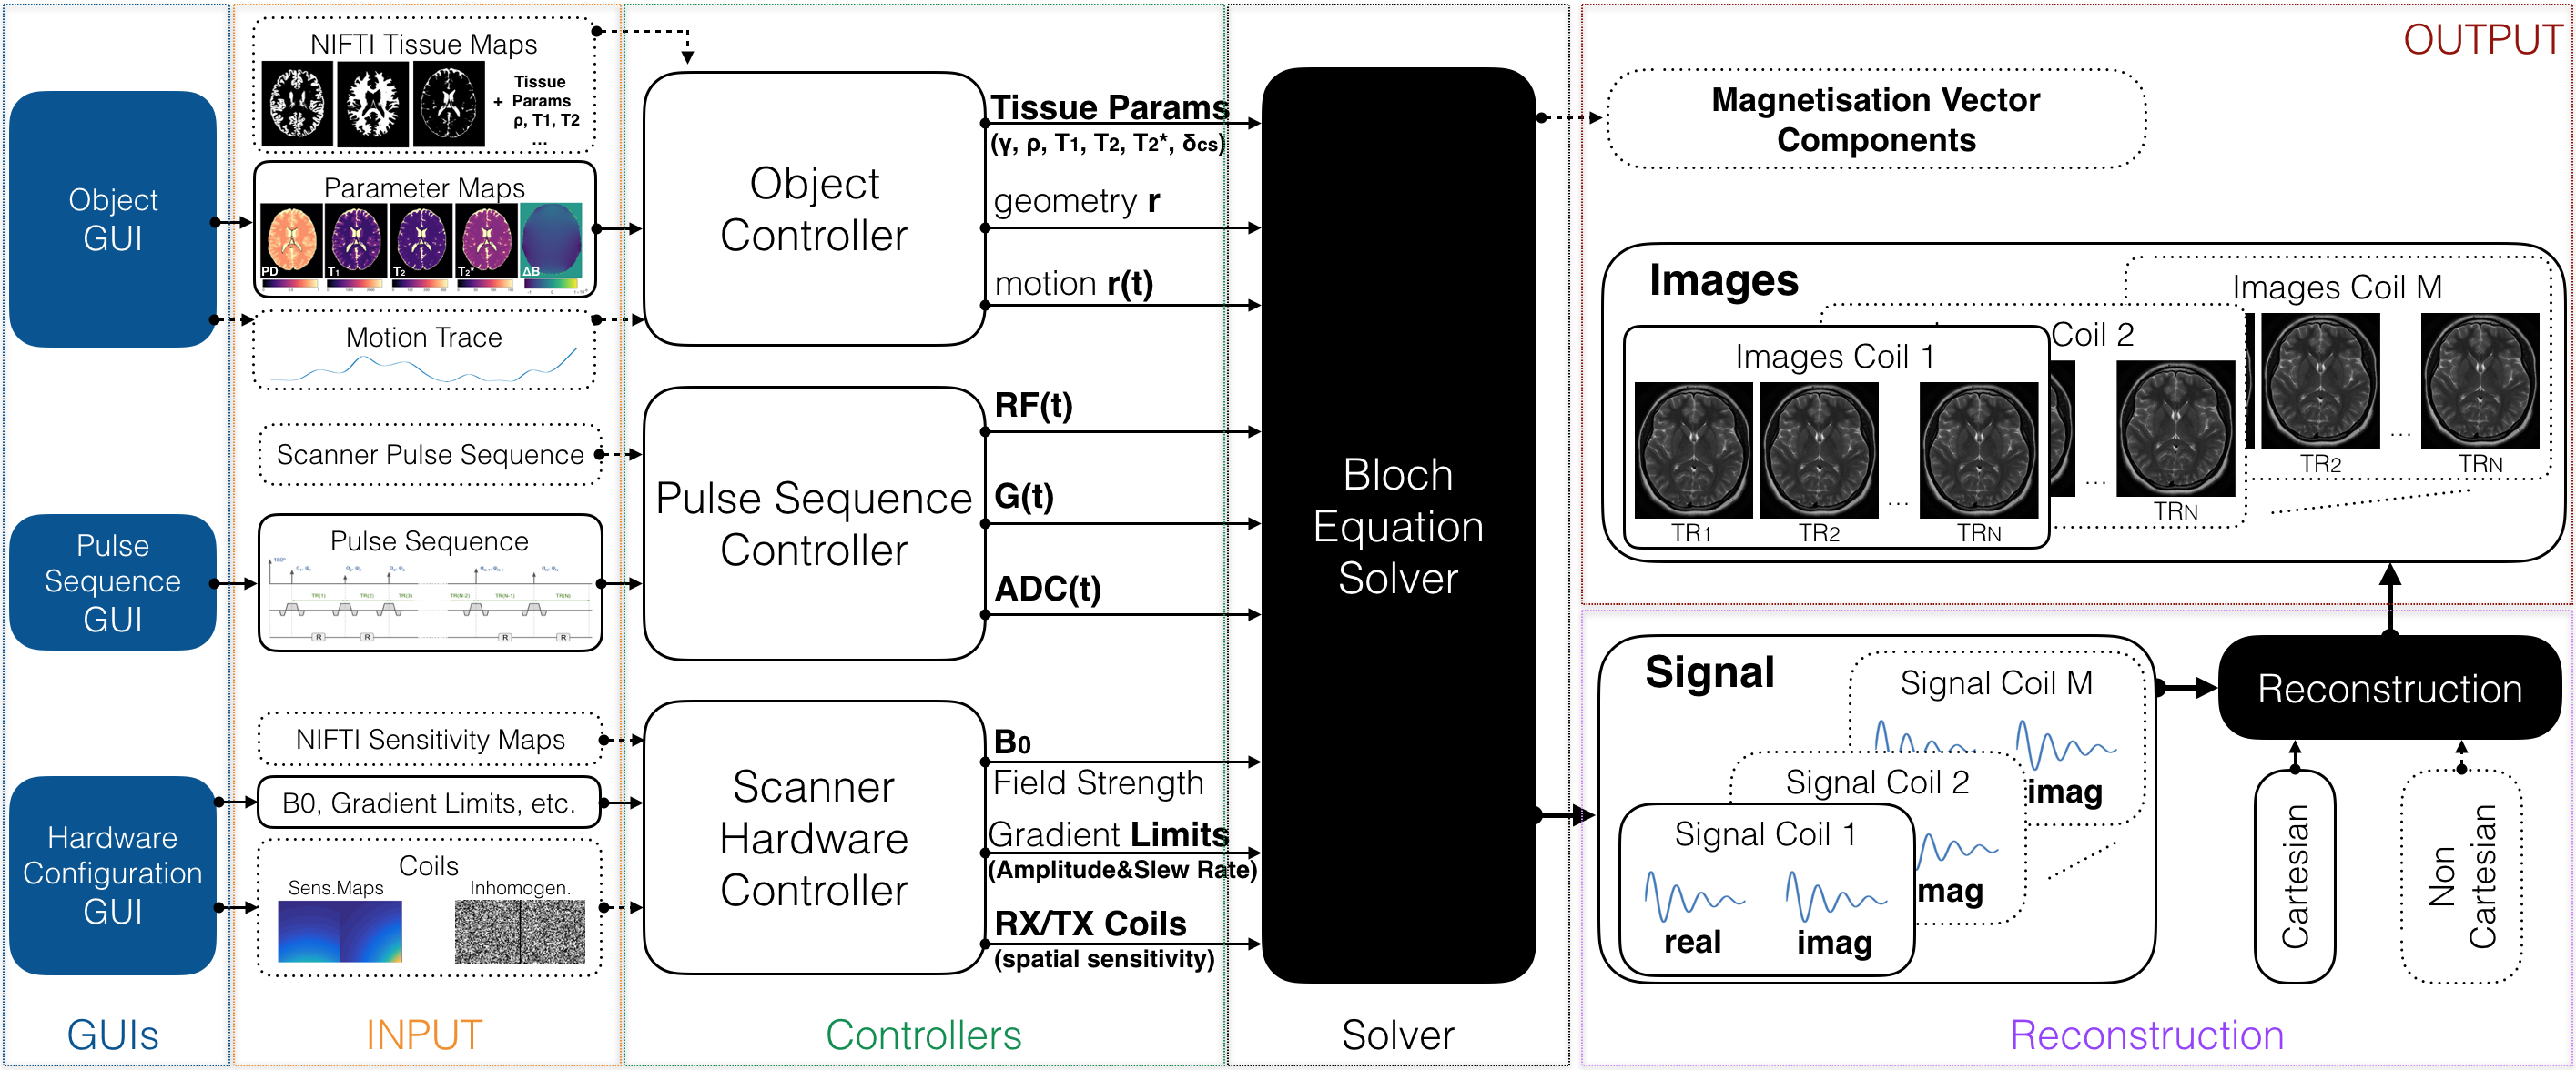
\includegraphics[angle=90,width=0.7\textwidth, keepaspectratio]{images/mri/globalFramework}
    \caption{Generalised framework for an ideal Magnetic Resonance Imaging simulator}
    \label{fig:globalFramework}
\end{figure}



%%%%%%%%%%%%%%%%%%%%%%%%%%%%%%
%% Appendices
%%%%%%%%%%%%%%%%%%%%%%%%%%%%%%
\addcontentsline{toc}{chapter}{Appendices}

% The \appendix command resets the chapter counter, and changes the chapter numbering scheme to capital letters.
%\chapter{Appendices}
\appendix
% % % % % % % % 
% % % % % % % % MRI background
% % % % % % % % 
\chapter{Principles of Magnetic Resonance Imaging}
\label{appendixlabelBackgroundMRI}

Magnetic Resonance Imaging (MRI) is a powerful and highly versatile imaging 
modality that uses the principles of nuclear magnetic resonance (NMR) 
first observed by Bloch and Purcell in 1946 \cite{Bloch1946} 
\cite{Purcell1946}.
This non-invasive imaging technique is able to produce images by spatially 
varying the phase and the frequency of the energy being absorbed and 
emitted by the imaged object, a technique that was proposed in 1973 
in the seminal papers by Lauterbur \cite{Lauterbur1973} and Mansfield \cite{Mansfield1973}. 
MRI relies on observing the way atomic nuclei 
respond and interact with an applied magnetic field. 
In clinical MRI, the focus is entirely on the hydrogen proton, 
the most abundant element in the human body. 
This provides the basis for the imaging techniques used and described in this thesis.

\hfill

This section gives an overview of the main principles involved in the 
formation of images using nuclear magnetic resonance (NMR). 
It begins with an explanation of the basic building blocks of NMR, % NMR
discusses the steps involved in image formation, % image formation
introduces the notion of k-space, % and its link with data sampling flexibility and restrictions, % data sampling
and discusses some of the main limitations of MRI.

% % % % % % % % % % % % % % % % 
\section{Nuclear Magnetic Resonance Physics}\label{chapterlabel2sec11}
The first step towards producing MR images is to understand the way protons respond to
external magnetic fields. 
This section gives an overview of the interaction between protons with different types of applied magnetic fields, as well as with its surroundings.

\hfill

% % % % % % % % % % % % 
% % % % % % % % % % % % 
\subsection{Magnetisation}

% % 1
\textbf{Magnetic moment.}
The story of magnetic resonance imaging starts with the discovery 
by Stern and Gerlach in the early 1920's of a fundamental property of an 
odd numbered atomic nucleus. This property is known as \textit{angular momentum $\vec{J}$} (or \textit{spin}) and, from a classical perspective, it gives rise to a small \textit{magnetic moment} $\vec{\mu}$. 

\hfill

\textbf{Gyromagnetic Ratio.}
The relationship between the spin and the magnetic moment is found from experiment: 
\begin{equation} \label{eq:21}
    \vec{\mu} = \gamma \vec{J}
\end{equation}
where $\gamma$ is known as the \textit{gyromagnetic ratio}.

For hydrogen nuclei, this constant is experimentally found to be:
\begin{equation} \label{eq:22}
    \gamma_{H} = 2.675 \times 10^8 \text{  } rad/s/T
\end{equation}
or, under its reduced form, as:
\begin{equation} \label{eq:23}
    \text{\sout{$\gamma$}}_H \equiv \frac{\gamma}{2 \pi} = 42.58 \text{  } MHz/T
\end{equation}
where T is Tesla, the unit for magnetic field strength, and it is the equivalent of $10,000$ Gauss \cite{Haacke1999}.

\hfill

% % 2
\textbf{Torque in an external magnetic field.}
Under normal circumstances, the magnetic moment of a proton can
point in any direction. 
However, when submerged in an external magnetic field $\vec{B}$, 
the magnetic moment vector of the proton spin will experience a 
non-zero torque $\vec{N}$ which will align the magnetic 
moment along the direction of the field:
\begin{equation} \label{eq:24}
    \vec{N} = \vec{\mu} \times \vec{B}
\end{equation}

% % 3
The total torque acting on a system is equal to the 
rate of change of angular momnetum with time \cite{Haacke1999}:
\begin{equation} \label{eq:25}
    \frac{d\vec{J}}{dt} = \vec{N}
\end{equation}

\hfill

\textbf{Equation of motion.} This equation, together with equations \ref{eq:24} and \ref{eq:21},
give rise to the \textit{fundamental equation of motion} for a single
spin immersed in a static magnetic field:
\begin{equation} \label{eq:26}
    \frac{d\vec{\mu}}{dt} = \gamma \vec{\mu} \times \vec{B}
\end{equation}

By forming a dot product of both sides of equation \ref{eq:26} we get that $\frac{d}{dt} (\vec{\mu} \cdot \vec{\mu}) = 0$ which means that the magnitude of the magnetic moment vector remains constant in time. Moreover, the equation of motion (equation \ref{eq:26}) says that the direction of the magnetic moment vector changes in time. This motion is called \textit{precession} and it is a clockwise rotation about the direction of the main magnetic field as seen in Figure~\ref{fig:ch2precession}.

\begin{figure}[ht]
    \centering
    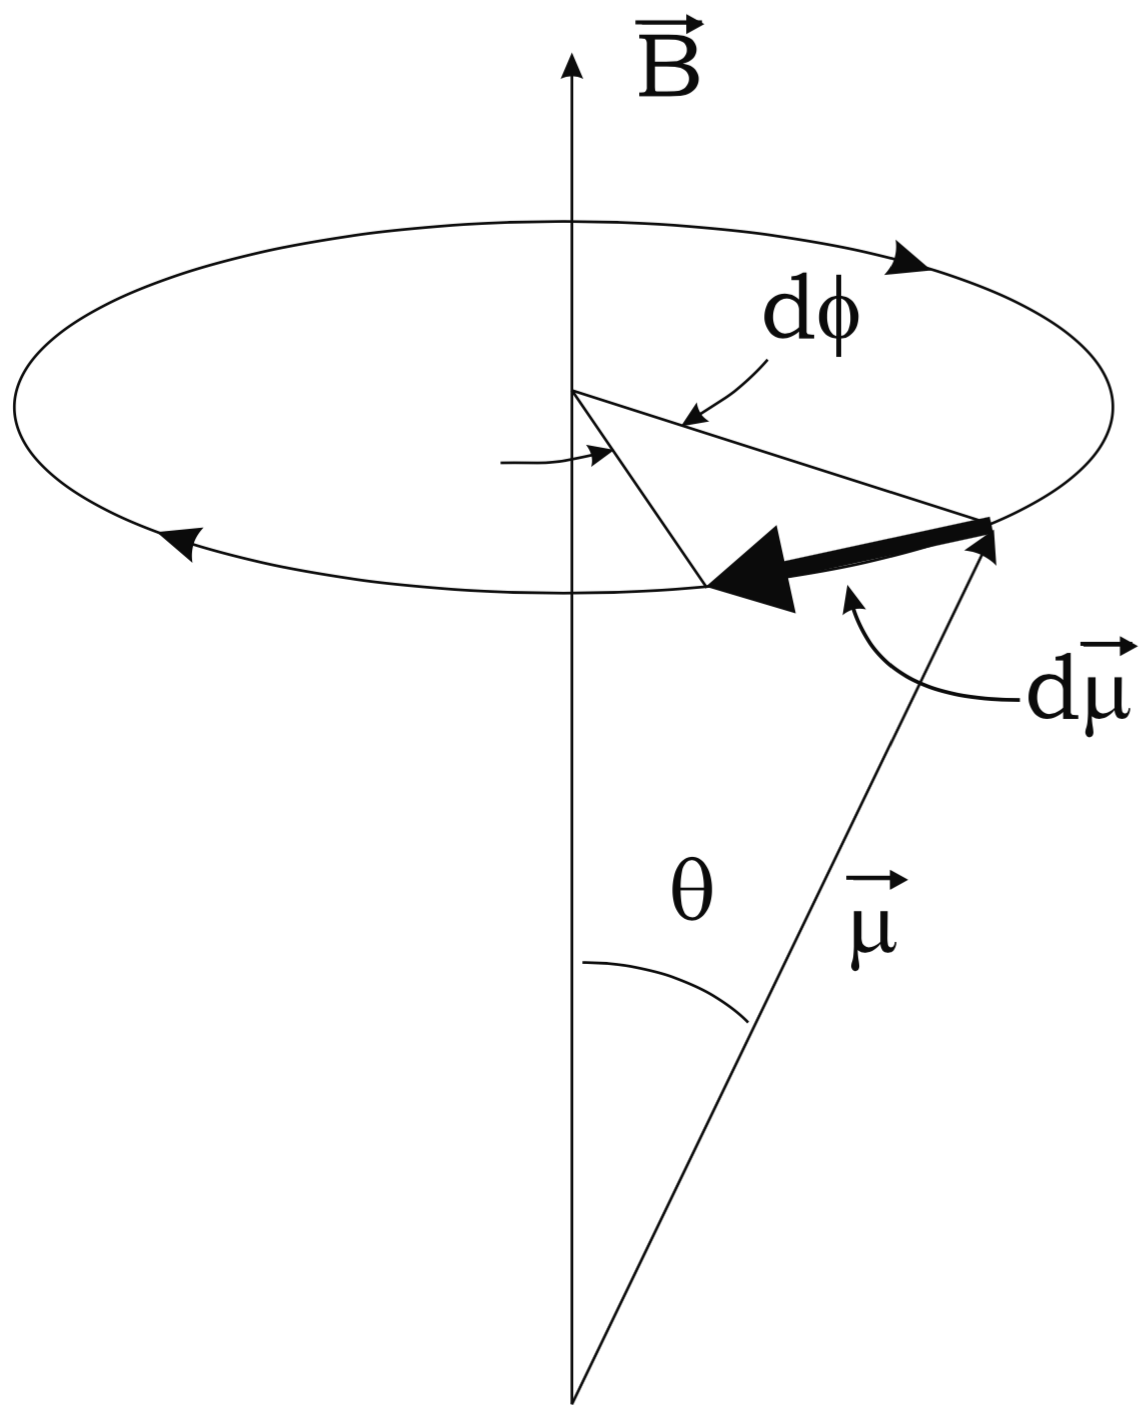
\includegraphics[width=0.4\textwidth,keepaspectratio]{images/mri/ch2precession}
    \caption{Clockwise precession of a proton's spin about a magnetic field. Figure adapted from \cite{Haacke1999}.}
    \label{fig:ch2precession}
\end{figure}

\hfill

% % 4
\textbf{Larmor frequency.} The angular frequency that the magnetic moment $\vec{\mu}$ precesses about the magnetic field in a clockwise fashion is called the \textit{Larmor frequency}:
\begin{equation} \label{eq:28}
	\omega \equiv \Bigl\vert \frac{d \phi}{dt} \Bigr\vert = \gamma \lvert \vec{B} \rvert
\end{equation}

\hfill

% % 5
\textbf{Cartesian representation.}
Considering a static magnetic field $\vec{B} = B_0 \hat{z}$, and a magnetic 
moment pointing in an arbitrary direction, the equation of motion
can be rewritten as follows:
\begin{flalign*}
    \frac{d}{dt}(\mu_x \hat{x} + \mu_y \hat{y} + \mu_z \hat{z}) & = \gamma\, B_0\, (\mu_x \hat{x} + \mu_y \hat{y} + \mu_z\hat{z}) \times \hat{z}\\
    & = \gamma\, B_0\, ( \mu_y \hat{x}  - \mu_x \hat{y} )
\end{flalign*}
The vector differential equation \ref{eq:26} will therefore decompose into 
the three Cartesian equations:
\begin{flalign*}
    \frac{d\mu_x}{dt} & = \phantom{+} \gamma \mu_y B_0 = \phantom{+} \omega_0\,\mu_y \\
    \frac{d\mu_y}{dt} & = - \gamma \mu_x B_0 = - \omega_0\,\mu_x \\
    \frac{d\mu_z}{dt} & = \phantom{+} 0
\end{flalign*}
whose solutions are:
\begin{flalign*}
    {\mu_x}(t) &= {\mu_x}(0) \, cos (\gamma B_0 t) + {\mu_y}(0) \, sin (\gamma B_0 t) \\
    {\mu_y}(t) &= {\mu_y}(0) \, cos (\gamma B_0 t) - {\mu_x}(0) \, sin (\gamma B_0 t) \\
    {\mu_z}(t) &= {\mu_z}(0)
\end{flalign*}

\hfill

% % 6
\textbf{Matrix representation.} A more concise representation of the equation 
of motion of a single spin in a static magnetic field is using matrix notation: 
\begin{equation} \label{eq:27}
	\vec{\mu}(t) = R_z(- \gamma B_0 t) \vec{\mu}(0)
\end{equation}
where 
\begin{flalign*}
	\vec{\mu}(t) & =
    \begin{pmatrix}
	\mu_x(t)\\
	\mu_y(t)\\
	\mu_z(t)
	\end{pmatrix} \text{ and } \omega_0 = -\gamma B_0
\end{flalign*}
and $R_z(\alpha)$ is the matrix representing the anti-clockwise rotation of vectors through an angle $\alpha$:
\begin{flalign*}
	R_z(\alpha) & =
    \begin{pmatrix}
	cos\alpha & -sin\alpha & 0 \\
	sin\alpha & \phantom{+}cos\alpha & 0 \\
	0 & 0 & 1
	\end{pmatrix}
\end{flalign*}
For completion, the rotations about the x and y axis are also presented here:
\begin{flalign*}
	R_x(\alpha) & =
    \begin{pmatrix}
	1 & 0 & 0 \\
	0 & cos\alpha & -sin\alpha \\
	0 & sin\alpha & \phantom{+}cos\alpha 
	\end{pmatrix}
\end{flalign*}
and
\begin{flalign*}
	R_y(\alpha) & =
    \begin{pmatrix}
    \phantom{+}cos\alpha & 0 & sin\alpha \\
	0 & 1 & 0 \\
	-sin\alpha & 0 & cos\alpha  
	\end{pmatrix}
\end{flalign*}

\hfill

% % 7
\textbf{Complex Representation.} Another useful representation of the magnetic moment vector is as a complex number:
\begin{equation} \label{eq:239}
	\mu_+ (t) = \mu_x(t) + i \mu_y(t)
\end{equation}
which allows a very concise representation of the equation of motion:
\begin{equation} \label{eq:240}
	\frac{d\mu_+}{dt} = - i \omega_0 \mu_+
\end{equation}
whose solution is:
\begin{equation} \label{eq:241}
	\mu_+(t) = \mu_+(0) e^{-i \omega_0 t}
\end{equation}

Similarly, by introducing phase into the equation we get:
\begin{equation} \label{eq:244}
	\mu_+(t) = \lvert \mu_+(0) \rvert e^{i \phi_0(t)}
\end{equation}
where the phase is:
\begin{equation} \label{eq:245}
	\phi_0(t) = -\omega_0 t + \phi_0(0)
\end{equation}

\hfill

% % 8
\textbf{Magnetisation.} The magnetic moment vectors of a population of spins 
(also known as an \textit{isochromat}) contained in a volume $V$ give rise to 
a net magnetisation. This vector quantity is called the 
\textit{magnetisation vector} and it is defined as:
\begin{equation} \label{eq:219}
    \vec{M} = \frac{1}{V} \sum_{i \in \text{protons in V}} \vec{\mu}_i
\end{equation}

The equation of motion for the magnetisation vector is the same as for a single spin:
\begin{equation} \label{eq:43}
    \frac{d\vec{M}}{dt} = \gamma \vec{M} \times \vec{B}  \text{  (for non-interacting protons)}
\end{equation}

At thermal equilibrium and when immersed in a constant, static magnetic field 
$\vec{B} = B_0 \, \hat{z}$, the magnetisation vector becomes $\vec{M} = M_0 \, \hat{z}$,
where $M_0$ is found from quantum statistics to be:

\begin{equation} \label{eq:225}
    M_0 = \frac{\gamma^2 \text{\sout{$h$}}^2 \, B_0 \, \rho}{4 \, K \, T}
\end{equation}

In equation \ref{eq:225} we introduced the following quantities: \sout{$h$} $= h/2\pi$ is the reduced Planck constant $h$ ($h = 6.626 \times 10^{-34} J$), also known as \textit{h-bar}, $\rho$ is the number of spins per unit volume 
(spin density), $K$ is the Boltzmann constant 
($1.38 \times 10^{-23} J \, K^{-1}$) and $T$ is the absolute temperature of the system \cite{Haacke1999}. \\

The magnetisation vector $M_0$ is the measured quantity in an MRI experiment. 
As this vector quantity is several orders of magnitude smaller than $B_0$, measuring it 
can only be done by lowering the overall temperature of the object or by increasing the field strength.
In fact, the only actual controllable parameter is the amplitude of the external magnetic field, or $B_0$, which in MRI scanners can range between 0.2 to 9 Tesla, with 1.5T and 3T scanners being the most popular clinically used ones.

\hfill

% % % % % % % % % % % % 
% % % % % % % % % % % % 
\subsection{Radiofrequency Pulse}\label{background:rfpulse}

As stated before, the measurable quantity in MRI is the net 
magnetisation vector. However, in order to be measured, 
the magnetisation vector must be 'tipped' away from its 
thermal equilibrium alignment.
This can be achieved by applying a secondary magnetic field known as the 
\textit{RF Pulse}.
The resulting combined effect of two perpendicular fields leads to a disturbance of any magnetic moment, initially aligned along the original static field, away from that direction. 

\hfill

% % 8
\textbf{Rotating reference frames.} 
The motion of the magnetisation vector while subject to these fields is best described using a new reference frame.
This reference frame is called the \textit{rotating reference frame} and can be distinguished from the \textit{laboratory frame} (stationary frame) by using primed quantities for both the axis of the frame ($x'$, $y'$, $z'$) and their respective unit vectors ($\hat{x}'$, $\hat{y}'$, $\hat{z}'$). 

\hfill

The rotation motion of this frame can be described by the angular velocity vector $\vec{\Omega}$ whose direction and magnitude are the rotation axis and the angular speed of the rotating frame. The rate of change of the magnetisation vector in time relative to the rotating reference frame can be expressed as:
\begin{equation}\label{eq:4433}
    \frac{d \vec{M} (t)}{dt} = \Bigg( \frac{d \vec{M} (t)}{dt} \Bigg)' + \vec{\Omega} \times \vec{M}(t)
\end{equation}

By using equation \ref{eq:43} together with the above equation we get:
\begin{equation}\label{eq:313}
    \Bigg( \frac{d \vec{M} (t)}{dt} \Bigg)' = \gamma \vec{M} \times \vec{B}_{eff}
\end{equation}
where the effective magnetic field in the rotating frame is:
\begin{equation}\label{eq:314}
    \vec{B}_{eff} = \vec{B} + \frac{\vec{\Omega}}{\gamma}
\end{equation}

This is a key equation in MR as it shows that from the primed reference frame perspective, the magnetisation vector is rotated due to the presence of a total (or effective) magnetic field. The choice of $\vec{\Omega}$ is then equal to $- \gamma \vec{B}$ such that the magnetisation vector will lie still in the rotating reference frame.

\hfill

% % 9
\textbf{RF Field.} By introducing a new magnetic field which is perpendicular to the main magnetic field, the magnetisation vector can be 'tipped' away from the $\hat{z}$ axis. This field is called the \textit{transmit RF field} ($\vec{B_1}$) and it is most effective when it is a \textit{left-circularly polarized} magnetic field. Specifically, the RF field used in MRI is:
\begin{equation}\label{eq:324}
    \vec{B}_{1}^{cir} = B_1 (\hat{x} \, cos \, \omega t - \hat{y} \, sin \, \omega t)
\end{equation}
which makes it static in the rotating reference frame:
\begin{equation}\label{eq:325}
    \vec{B}_{1}^{cir} = B_1 \hat{x}'
\end{equation}

When combining the constant magnetic field $\vec{B_0} = B_0 \hat{z}$ with the left-circularly polarised field $\vec{B_1} = B_1 \hat{x}'$ and setting $\hat{z}' = \hat{z}$ we get:
\begin{equation}\label{eq:326}
    \Bigg( \frac{d \vec{M} }{dt} \Bigg)' = \vec{M} \times [ \hat{z}'  (\omega_0 - \omega) + \hat{x}' \omega_1]
\end{equation}
where $\omega_0 \equiv \gamma B_0$ is the Larmor frequency, $\omega$ is the rf laboratory frequency and $\omega_1 \equiv \gamma B_1$ is the precession frequency induced by the rf field.

The effective magnetic field will therefore be:
\begin{equation}\label{eq:328}
    \vec{B}_{eff} \equiv [ \hat{z}'  (\omega_0 - \omega) + \hat{x}' \omega_1] / \gamma
\end{equation}

\hfill

% % 10
\textbf{On-resonance Condition.} 
In MRI the applied RF field's frequency $\omega$ is chose such that it matches the Larmor frequency $\omega_0$. 
This is called the \textit{on-resonance condition} and it leads to the cornerstone equation of motion:
\begin{equation}\label{eq:329}
    \Bigg( \frac{d \vec{M}}{dt} \Bigg)' = \omega_1 \vec{M} \times \hat{x}'
\end{equation}
where the $B_1$ field is maximally synchronised to tip the spin about the $\hat{x}'$ axis.

\hfill

% % 11
\textbf{RF Pulse.} \label{app:rfpulse}
An on-resonance RF transmit field applied for a finite time is called an \textit{rf pulse}. 
The magnitude of the $B_1$ field and the amount of time $\tau$ it is turned on can be adjusted to control for the angle of rotation. 
This angle is called \textit{flip angle} and is related to the other two quantities through the following formula:
\begin{equation}\label{eq:331}
    \Delta \theta = \gamma B_1 \tau
\end{equation}
For example, a $\pi/2$ flip can be achieved in $1.0 ms$ with a $B_1$ field of $5.9 \mu T$ for hydrogen protons \cite{Haacke1999}. 
The trajectory of the magnetisation vector undergoing this motion is illustrated in Figure~\ref{fig:ch3spintrajboth}.

\begin{figure}[ht]
    \centering
    \begin{subfigure}[b]{0.45\textwidth}
        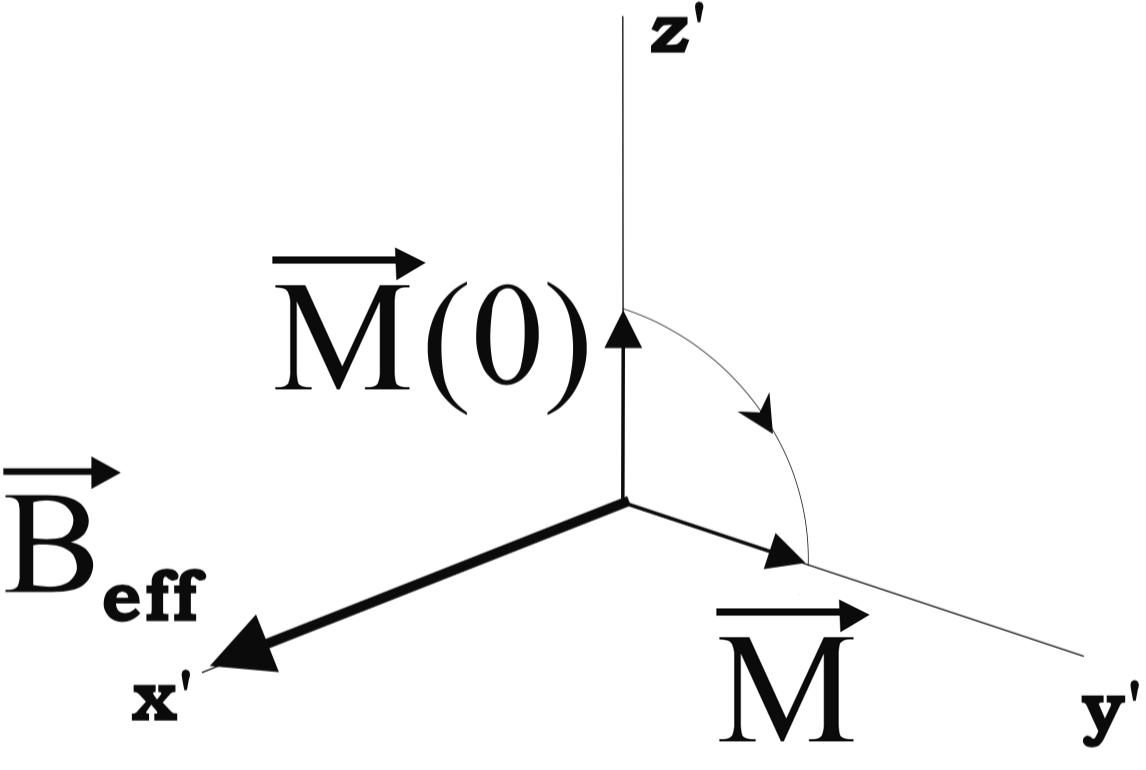
\includegraphics[width=\textwidth]{images/mri/ch3spintraja}
        \caption{Rotating frame}
        \label{fig:ch3spintraja}
    \end{subfigure}
    ~ %add desired spacing between images, e. g. ~, \quad, \qquad, \hfill etc. 
      %(or a blank line to force the subfigure onto a new line)
    \begin{subfigure}[b]{0.4\textwidth}
        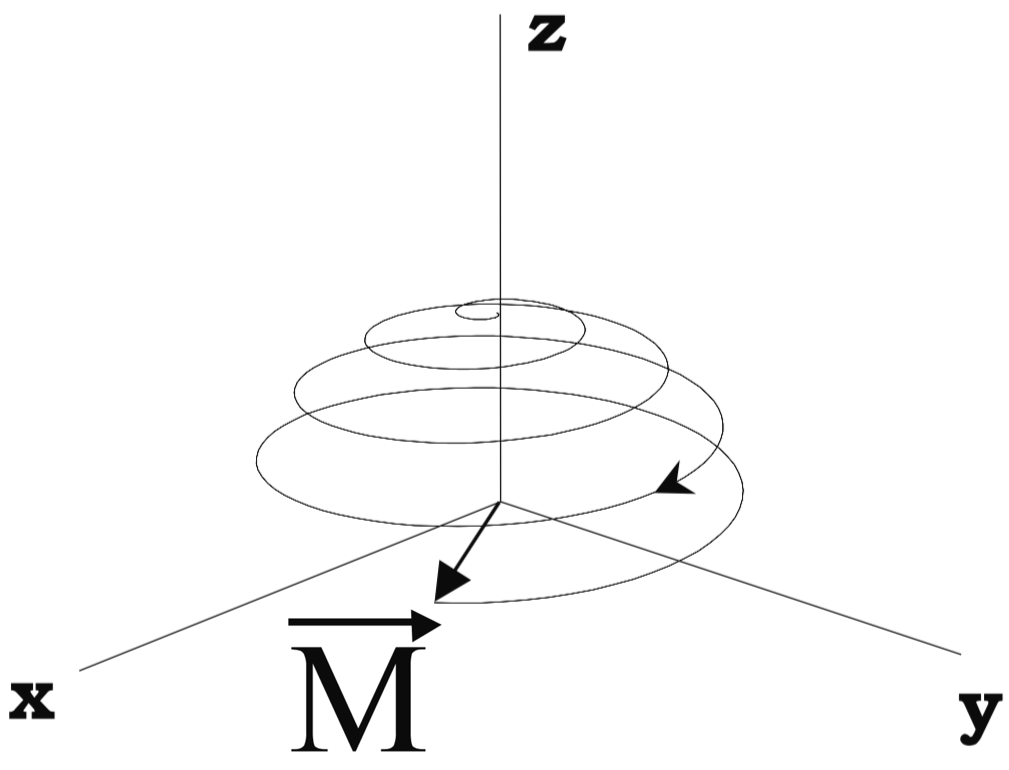
\includegraphics[width=\textwidth]{images/mri/ch3spintrajb}
        \caption{Laboratory frame}
        \label{fig:ch3spintrajb}
    \end{subfigure}
    
    \caption{Magnetisation vector trajectory in both the rotating and the laboratory frame. Figure adapted from \cite{Haacke1999}}
    \label{fig:ch3spintrajboth}
\end{figure}

\hfill

In most MR experiments, the RF pulse has a very short duration (a few milliseconds).
It can therefore be assumed that it happens instantaneously and that there are no relaxation effects during it application.
Mathematically, an instantaneous RF pulse of flip angle $\alpha$ and initial phase $\phi$ can be described with rotation matrices.
The post-RF pulse magnetisation vector $\vec{M}$ will therefore depend on its pre-RF pulse state $\vec{M}(0)$ by the following equation
\begin{equation} \label{eq:445}
    M = R_z(\phi) R_x(-\alpha) R_z(-\phi) M(0)
\end{equation}

For a perfect $\pi/2$ pulse applied uniformly over the sample, the post-RF magnetisation vector will be the equilibrium magnetisation $M_0$. 
From equation ~\ref{eq:225} we can now write:
\begin{equation}\label{eq:93}
    M_{\perp}(\vec{r},0) = M_0(\vec{r}) = \rho_0(\vec{r}) \frac{\gamma^2 \text{\sout{$h$}}^2 \, B_0}{4 \, K \, T}
\end{equation}
which introduces the spin density $\rho_0$.

\hfill

% % % % % % % % % % % % 
% % % % % % % % % % % % 
\subsection{Relaxation} \label{app:relaxation}

The picture we have painted so far refers to non-interacting spins.
As expressed in equation \ref{eq:43}, the equation of motion for the magnetisation vector is $\frac{d\vec{M}}{dt} = \gamma \vec{M} \times \vec{B}$  for non-interacting protons. 
This equation can be decomposed into its parallel ($\vec{M}_{||} = M_z \hat{z}$) and longitudinal ($\vec{M}_{\perp} = M_X \hat{x} + M_y \hat{y}$) components which yield the following decoupled equations:
\begin{equation}\label{eq:46}
    \frac{d M_z}{dt} = 0
\end{equation}
and 
\begin{equation}\label{eq:47}
    \frac{d \vec{M}_{\perp}}{dt} = \gamma \vec{M}_{\perp} \times \vec{B}_{ext}
\end{equation}
for non-interacting protons.

\hfill

% % 12
\textbf{Interacting protons.} In reality, the hydrogen protons contained in a sample are constantly interacting with their environment and with each other.
The result of this interaction leads to additional terms in the equations above.
These terms will depend on some decay parameters which are different for both these equations.
This means that the magnetisation vector components will 'relax' differently to their equilibrium values.

\hfill

% % 13
\textbf{Spin-Lattice Relaxation.} The relaxation of the longitudinal component to its thermal equilibrium is called the \textit{spin-lattice relaxation}. 
When the magnetisation is disturbed by an external magnetic field such as an RF pulse, the spin system gains potential energy.
By releasing this energy back to the lattice, the magnetisation then returns to its equilibrium.
This process takes the form of an exponential recovery and it is described by the following empirical relation:
\begin{equation}\label{eq:411}
    \frac{d \vec{M}_{z}}{dt} = \frac{1}{T_1} (M_0 - M_z) \hat{z}
\end{equation}
where $T_1$ is known as the \textit{spin-lattice relaxation time} and its solution is:
\begin{equation}\label{eq:413}
    M_z(t) = M_z(0) e^{-t/T_1} + M_0(1-e^{-t/T_1}) \, \text{ (for } \vec{B}_0 \parallel \hat{z} \text{)}
\end{equation}

\hfill

% % 14
\textbf{Spin-Spin Relaxation.} The relaxation of the transverse component to its thermal equilibrium is called the \textit{spin-spin relaxation}. 
This phenomena happens due to the interaction between individual spins.
These interactions cause local magnetic field changes which lead to variations in the precessional frequencies of the spins.
As a consequence, the magnetic moment vectors will gain or lose phase with respect to the expected Larmor frequency.
Over time, this process will cause a complete dephasing of the system which will, in turn, lead to a zero net magnetisation vector.
To characterize this phenomena we use the $T_2$ \textit{spin-spin relaxation time} and the following empirical relation:
\begin{equation}\label{eq:412}
    \frac{d \vec{M}_{\perp}}{dt} = \gamma \vec{M} \times \vec{B} - \frac{1}{T_2} \vec{M}_{\perp}
\end{equation}
with solution:
\begin{equation}\label{eq:414}
    \vec{M}_{\perp}(t) = \vec{M}_{\perp}(0) e^{-t/T_2} \, \text{ (in the rotating frame)}
\end{equation}

\hfill

% % 15
\textbf{The $\mathbf{T_2^*}$ relaxation term.} 
In reality, the transverse relaxation rate is higher than described above because of external field inhomogeneities.
This process is characterised by a separate decay rate called $R_2' \equiv 1/T_2'$ and together with the intrinsic decay rate $R_2 \equiv 1/T_2$ yields the total relaxation rate $R_2^* = R_2 + R_2'$.
By inverting this equation we arrive with:
\begin{equation} \label{eq:420}
    \frac{1}{T_2^*} = \frac{1}{T_2} + \frac{1}{T_2'}
\end{equation}
where ${T_2^*} \equiv 1/R_2^*$.
It is worth mentioning that the loss in transverse magnetisation due to external field inhomogeneities $T_2'$ is 'recoverable' in MRI, while the intrinsic $T_2$ losses are not.

\hfill

% % % % % % % % % % % % 
% % % % % % % % % % % % 
\subsection{Off-resonance Effects}

These inhomogeneities directly affect the spins' precession frequencies.
As stated before, the frequency of precession for a given spin is proportional to the gyromagnetic ratio and the magnitude of the magnetic field (equation \ref{eq:28}).
Any deviation from the expected $B_0$ value will therefore change the precession frequency to:
\begin{equation}
    \omega = \gamma \lvert \vec{B}_0 + \Delta \vec{B} \rvert = \omega_0 + \Delta \omega
\end{equation}
where $\Delta \omega$ is the off-resonance frequency.

\hfill

% % % % % % % % % % % % 
% % % % % % % % % % % % 
\label{chapterlabel2sec1Bloch}

The combined effect of both spin-lattice and spin-spin relaxations in one equation is called \textit{the Bloch equation}. 
This equation takes the following form:

\begin{equation} \label{eq:421}
    \frac{d\vec{M}}{dt} = \gamma \vec{M} \times \vec{B} + \frac{1}{T_1} (M_0 - M_z) \hat{z} - \frac{1}{T_2} \vec{M}_{\perp}
\end{equation} 

which can be decomposed in its $x/y/z$ components:
\begin{equation} \label{eq:422}
    \frac{dM_z}{dt} = \frac{M_0 - M_z}{T_1}
\end{equation}
\begin{equation} \label{eq:423}
    \frac{dM_x}{dt} = \omega_0 M_y - \frac{M_x}{T_2}
\end{equation}
\begin{equation} \label{eq:424}
    \frac{dM_x}{dt} = -\omega_0 M_x - \frac{M_y}{T_2}
\end{equation}
for $\vec{B} = B_0 \hat{z}$ and $\omega_0 = \gamma B_0$.

\hfill

% % 15
\textbf{Solutions to the Bloch equation.} 
The solutions for the equations above are:
\begin{equation} \label{eq:425}
    M_x(t) = e^{-t/T_2} (M_x(0) \, cos \, \omega_0 t + M_y(0) \, sin \, \omega_0 t)
\end{equation}
\begin{equation} \label{eq:426}
    M_y(t) = e^{-t/T_2} (M_y(0) \, cos \, \omega_0 t - M_x(0) \, sin \, \omega_0 t)
\end{equation}
\begin{equation} \label{eq:427}
    M_z(t) = M_z(0) e^{-t/T_1} + M_0 (1 - e^{-t/T_1})
\end{equation}
which reach $M_x(\infty) = M_y(\infty) = 0$ and $M_z(\infty) = M_0$ in the asymptotic limit $t \rightarrow \infty$.

Figure~\ref{fig:ch4MxMyMz} shows the behaviour of the magnetisation vector components in time for a sample with $T_1 = 600 \, ms$ and $T_2 = 80 \, ms$ at $B_0 = 1.5T$, which corresponds to white matter.

\begin{figure}[ht]
    \centering
    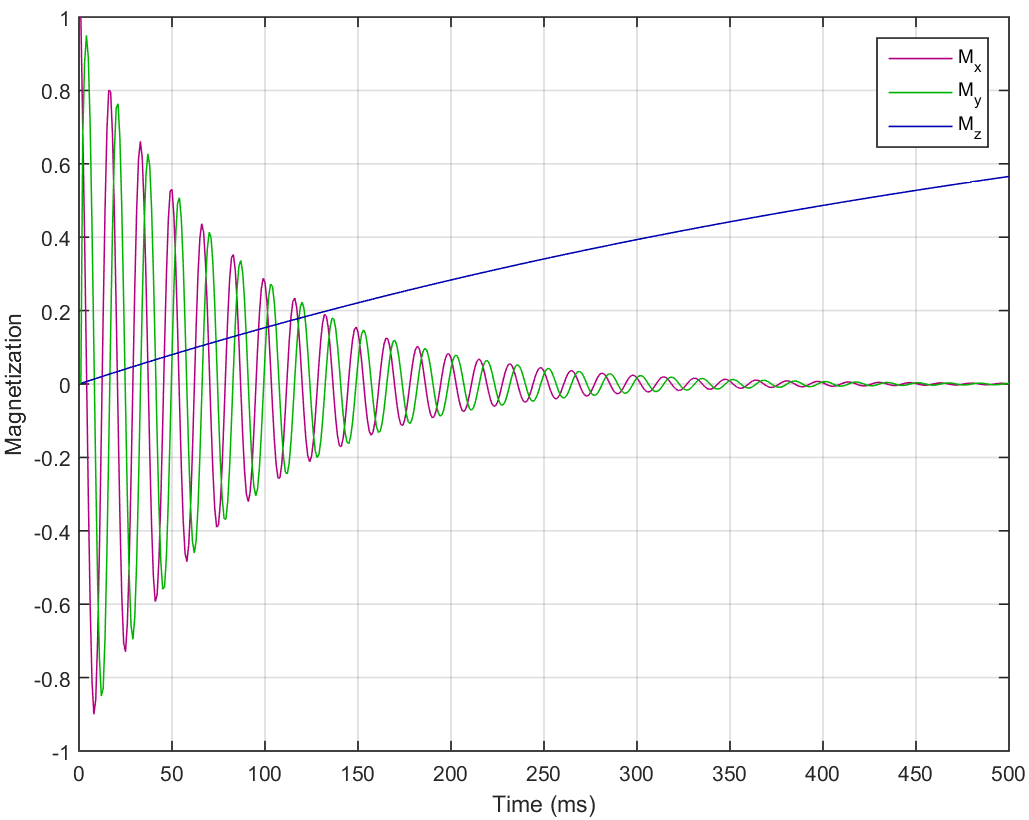
\includegraphics[width=0.9\textwidth,keepaspectratio]{images/mri/ch4MxMyMz}
    \caption{Relaxation in the laboratory frame. This figure shows the regrowth of the longitudinal component of the magnetization vector from 0 to its initial value $M_0$ in blue and the decay of both transverse components from an initial value to 0 in purple and green. $M_0$ is considered to be equal to 1 for illustration purposes.}
    \label{fig:ch4MxMyMz}
\end{figure}

\hfill

% % 16
\textbf{Matrix representation.} A useful representation for the Bloch equation is the \textit{matrix representation}.
By constructing a diagonal matrix $D$ with the $T_1$ and $T_2$ decay factors:
\begin{equation}
    D ( t ) = \left[
    \begin{array}{c c c}
          e^{-t/T_2} &     0      &     0 \\
              0      & e^{-t/T_2} &     0 \\
              0      &     0      & e^{-t/T_1}
    \end{array}
    \right]
\end{equation}
a column matrix $C$:
\begin{equation}
    C ( t ) = \left[
    \begin{array}{c}
        0 \\
        0 \\
    M_0(1 - e^{-t/T_1})
    \end{array}
    \right]
\end{equation}
and the previously defined rotation matrix $R_z$ we get:

\begin{equation} \label{eq:444}
    M(t) = D(t) R_z(-\omega_0 t) M(0) + C(t)
\end{equation}
where $M(t)$ is:
\begin{equation}
    M ( t ) = \left[
    \begin{array}{c}
        M_x(t) \\
        M_y(t) \\
        M_z(t)
    \end{array}
    \right]
\end{equation}
and $M(0)$ is the magnetisation vector immediately after it has been flipped by an instantaneous RF pulse.

% % % % % % % % % % % % % % % % 
\section{Image Formation}\label{chapterlabel2sec12}
After establishing the mathematical framework for how protons react to being subjected to a variety of magnetic fields we are now in the position of discussing how images are formed in MRI.
This section focuses on describing how MR images are obtained, from signal acquisition to image reconstruction. 

\hfill

% % % % % % % % % % % % 
% % % % % % % % % % % % 
\subsection{Signal Detection}

An important step towards image formation is the signal acquisition process. 
The precession motion of the magnetisation vector in the transverse plane can be detected by measuring the induced voltage in a receiver coil. 
The law that governs this phenomena is called the \textit{Faraday's lay of electromagnetic induction}.
It states that the induced voltage (\textit{emf}) is proportional to the rate of change of the magnetic flux ($\Phi$) through the coil:
\begin{equation} \label{eq:71}
    emf = - \frac{d \Phi(t)}{dt}
\end{equation}
where 
\begin{equation}\label{eq:72}
    \Phi(t) = \int_{sample} \vec{B}^{receive}(\vec{r}) \cdot \vec{M}(\vec{r}, t) d\vec{r}
\end{equation}
and $\vec{B}^{receive}(\vec{r})$ is the detection coil's 'received' magnetic field at position $\vec{r}$, and $\vec{M}(\vec{r}, t)$ is the magnetization vector at position $\vec{r}$ and time $t$.
A full derivation of equation \ref{eq:72} can be found in \cite{Haacke1999}. 
The signal through time $S(t)$ is proportional to the electromotive force:
\begin{equation}\label{eq:714}
    S(t) \propto V(t) = - \frac{d }{d t} \int_{sample} \vec{B}^{receive}(\vec{r}) \cdot \vec{M}(\vec{r}, t) d\vec{r}
\end{equation}
which in its decomposed form looks like:
\begin{equation}
    S(t) \propto - \frac{d}{dt} 
    \int_{sample}
          [B_x^{receive} (\vec{r}) M_x (\vec{r}, t) + 
          B_y^{receive} (\vec{r}) M_y (\vec{r}, t) + 
          B_z^{receive} (\vec{r}) M_z (\vec{r}, t)]  d\vec{r}
\end{equation}

After further simplifications and derivations, the details of which can be found in \cite{Haacke1999}, the signal expression known in MRI becomes:
\begin{equation}
    S(t) =
        \omega_0 \int_{sample} e^{-t/T_2(\vec{r})} M_{\perp}(\vec{r},0) 
            B_{\perp}(\vec{r}) sin(\omega_0 t + \theta_B(\vec{r}) - \phi_0(\vec{r})) d\vec{r}
\end{equation}
where $\phi_0$ is the initial phase of $\vec{M}_{\perp}$ after the RF pulse 
and $\theta_B$ is the receive field angle.
The equation can be modified to incorporate external field inhomogeneities by replacing $T_2$ with $T_2^*$.

\hfill

% % 17
\textbf{Signal demodulation.} In order to view the signal from the perspective of a rotating reference frame, the rapid $\omega_0$ oscillations are removed through a process called \textit{demodulation}.
In short, the signal is multiplied with a (co)sinusoid with a frequency that matches the $\omega_0$ Larmor frequency as close as possible.
The result of this process results in both a 'real' and an 'imaginary' channel for the signal.

By representing the magnetisation vector in its complex form:
\begin{equation}\label{eq:716}
\begin{aligned}
    M_{+}(\vec{r},t) \equiv M_x(\vec{r},t) + i M_y(\vec{r},t) &= e^{- t/T_2(\vec{r})} e^{-i \omega_0 t } M_+(\vec{r},0) \\
    &= e^{- t/T_2(\vec{r})} e^{-i \omega_0 t + i \phi_0(\vec{r})} M_{\perp}(\vec{r},0)
\end{aligned}
\end{equation}
as well as the receive field:
\begin{equation}\label{eq:729}
    B_{+} \equiv B_x^{receive} + i B_y^{receive} = B_{\perp} e^{i \theta_B}
\end{equation}
the compound complex signal becomes:
\begin{equation}\label{eq:730}
    s(t) \equiv s_{re}(t) + i s_{im}(t) \propto \omega_0 \int d^3 r \, \,  M_{+}(\vec{r},t) B^*_{+}(\vec{r})
\end{equation}

\hfill

% % % % % % % % % % % % 
% % % % % % % % % % % % 
\subsection{Spatial Encoding and K-Space Representation}

The signal we described so far is the global signal arising from the entire sample.
However, the goal of MRI is to determine the spatial distribution of the spins.
This can be achieved through spatially varying the magnetic field in such a way that different spins will precess at different rates based on their locations.

\hfill 

% % % % 
\textbf{Imaging Gradients} These variations in the main magnetic field can be achieved through \textit{gradient fields} which are defined by:
\begin{equation}
    \begin{split}
        \vec{G}(t) & \equiv \nabla B_{G_z}(\vec{r}, t) \\
                  &    =   \frac{\partial B_{G_z}(\vec{r},t)}{\partial x} \hat{x} + \frac{\partial B_{G_z}(\vec{r},t)}{\partial y} \hat{y} + \frac{\partial B_{G_z}(\vec{r},t)}{\partial z} \hat{z} \\
                  & \equiv G_x(t) \hat{x} + G_y(t) \hat{y} + G_z(t) \hat{z}
    \end{split}
\end{equation}
where $\vec{r}$ is a displacement vector from the isocenter and 
$G_x$, $G_y$ and $G_z$ are the components of the gradient field $\vec{G}$.
When a gradient field is superimposed over the main magnetic field, 
the total magnetic field at any location $\vec{r}$ is given by:
\begin{equation}
    \vec{B}(\vec{r},t) = (B_0 + \vec{G}(t) \cdot \vec{r}) \hat{z} = (B_0 + B_{G_z}(\vec{r}, t))\hat{z} = (B_0 + G_x(t)x + G_y(t)y + G_z(t)z) \hat{z}
\end{equation}

This equation can be rewritten in terms of the angular frequency of the precessing spins:
\begin{equation} \label{eq:910}
    \omega(\vec{r}, t) = \gamma \lvert \vec{B}(\vec{r}, t) \rvert = \gamma B_0 + \gamma B_{G_z} (\vec{r}, t) = \omega_0 + \gamma \vec{G}(t) \cdot \vec{r}
\end{equation}
which makes the connection between spatial coordinates and frequency of precession.

\hfill

% % % % 
\textbf{Spatial Selectivity}
In order to excite a certain part of the sample (slice selection), an RF pulse is applied together with a magnetic field gradient.
The angular frequency of the spins at location $z$ is given by the following equation:
\begin{equation} \label{eq:911}
    \omega(z) = \gamma B_0 + \gamma \vec{G} \cdot \vec{r} = \omega_0 + \gamma G_z z
\end{equation}
which, in frequency terms, becomes:
\begin{equation} \label{eq:912}
    \nu(z) = \nu_0 + \text{\sout{$\gamma$} } G_z z
\end{equation}
where $\nu_0$ is the frequency of the spins at the isocenter.

\hfill

The slice selection process can be modified to excite any slice at position $\delta z$ from the isocenter by changing the carrier frequency of the RF pulse with the offset $\delta \nu_{RF}$:
\begin{equation} \label{eq:913}
    \delta \nu_{RF} = \text{\sout{$\gamma$} } G_z \delta z
\end{equation}
The thickness of the slice is controlled by the RF pulse's transmit bandwidth of frequencies $\Delta \nu_{RF}$:
\begin{equation} \label{eq:914}
    \Delta z = \frac{\Delta \nu_{RF}}{\text{\sout{$\gamma$} } G_z} 
\end{equation}

The relationship between these terms can be seen in Figure~\ref{fig:ch9sliceselect}.

\begin{figure}[ht]
    \centering
    \begin{subfigure}[b]{0.48\textwidth}
        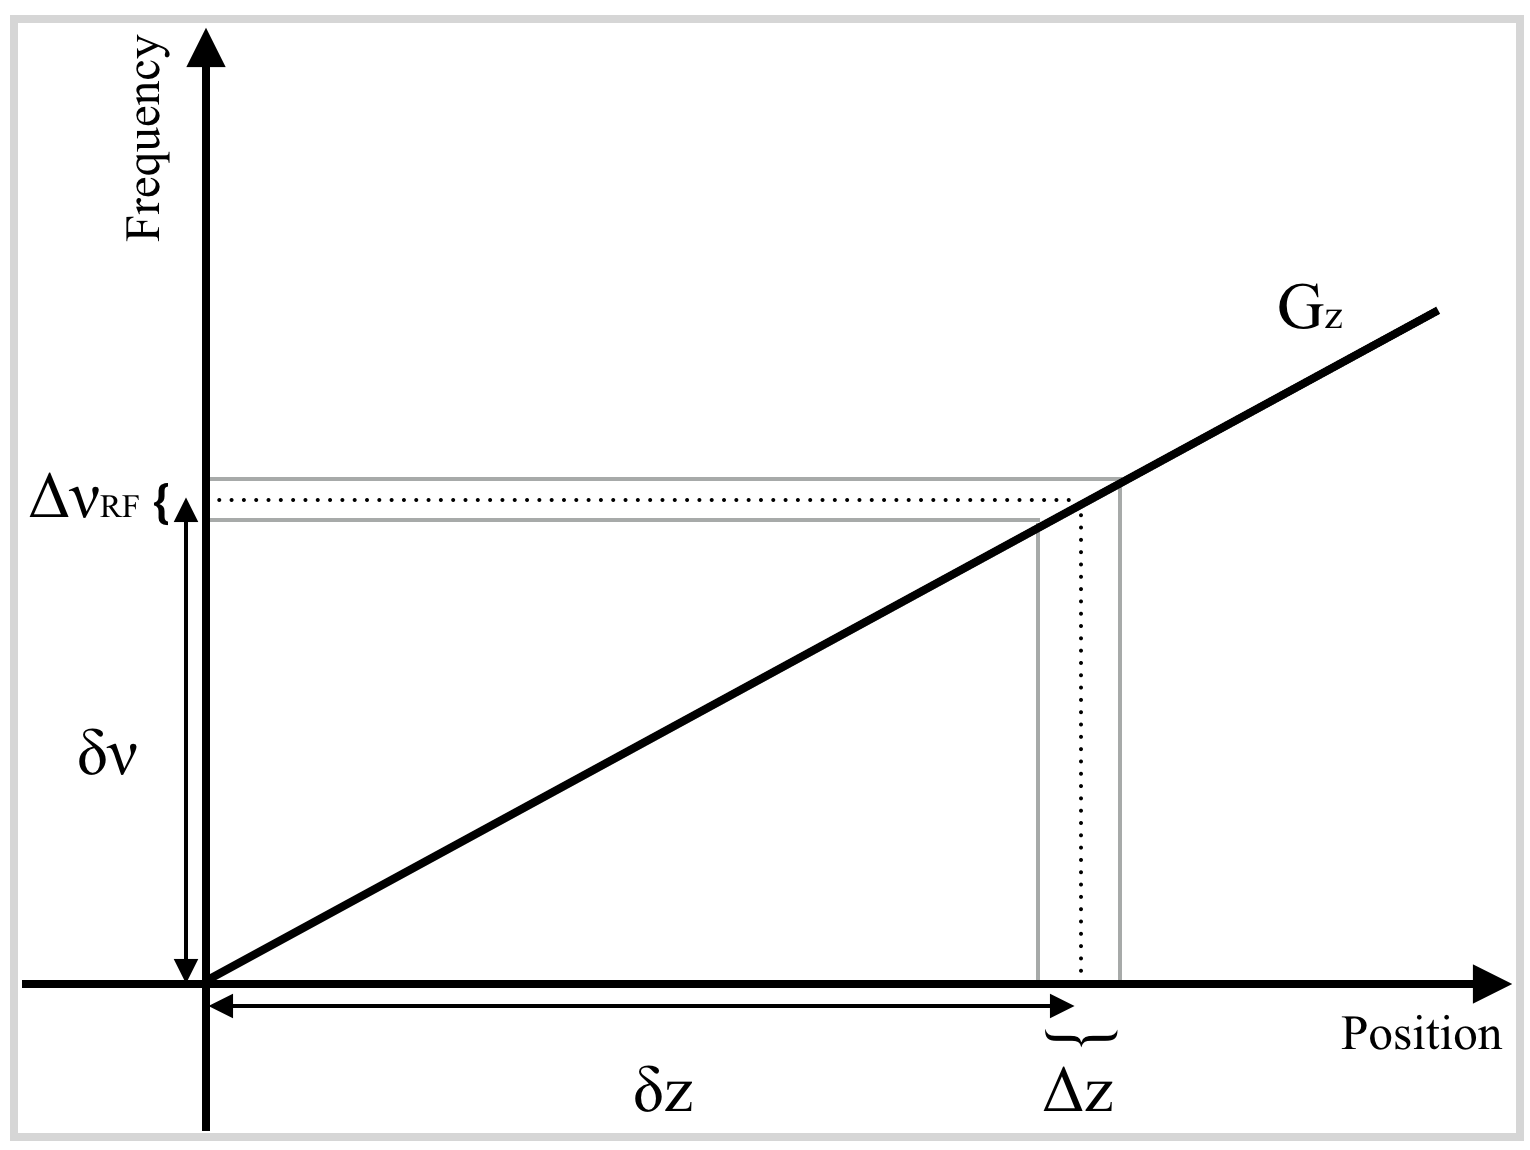
\includegraphics[width=\textwidth]{images/mri/ch9sliceselect1}
        \caption{Selection of slice at position $\delta z$ from the isocentre.}
        \label{fig:ch9sliceselect1}
    \end{subfigure}
    ~ %add desired spacing between images, e. g. ~, \quad, \qquad, \hfill etc. 
      %(or a blank line to force the subfigure onto a new line)
    \begin{subfigure}[b]{0.48\textwidth}
        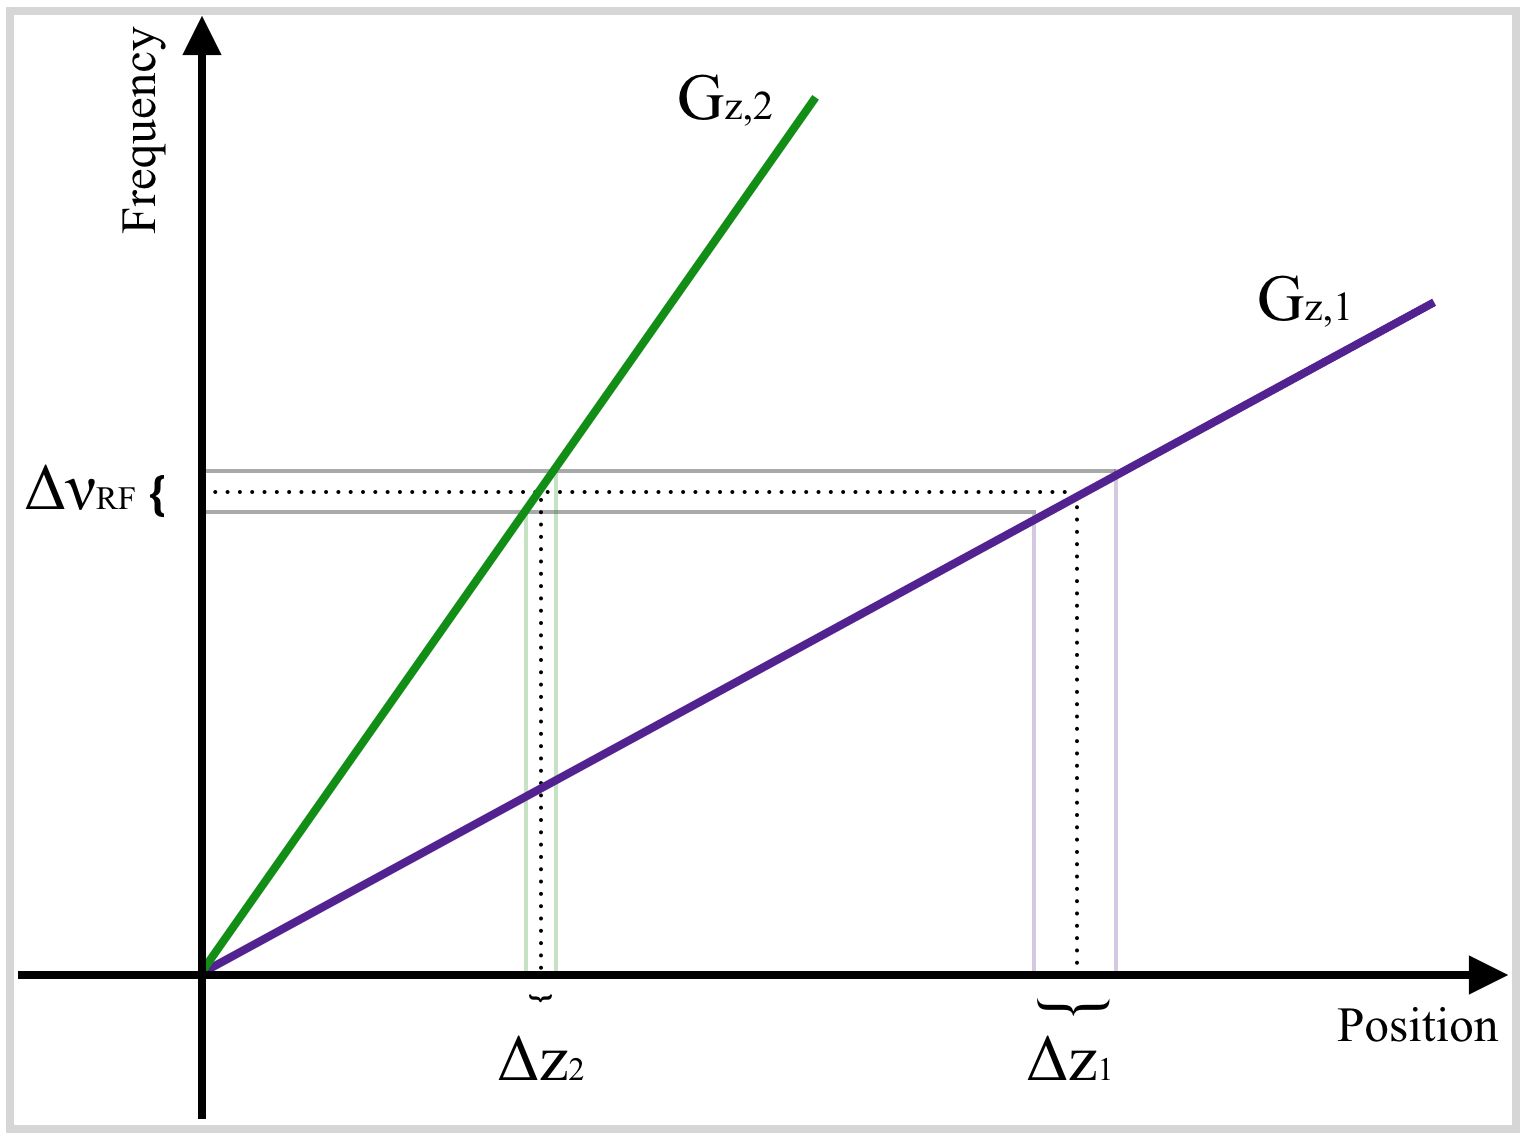
\includegraphics[width=\textwidth]{images/mri/ch9sliceselect2}
        \caption{Selection of slice thickness by controlling the gradient's strength.}
        \label{fig:ch9sliceselect2}
    \end{subfigure}
    
    \caption{The relationship between gradient strength, carrier frequency offset, frequency bandwidth, slice thickness and slice localistion.}
    \label{fig:ch9sliceselect}
\end{figure}

\hfill

% % % % 
\textbf{Frequency Encoding} After the selection of a certain slice, spatial encoding within the plane is performed. 
The first step of that process is called \textit{frequency encoding} and it is achieved by applying a linear gradient in one of the plane's directions.
For example, for a gradient $\vec{G}_{FE}$, the frequency of the spins will be linearly dependent the gradient's direction:
\begin{equation}
    \omega(\vec{r},t) = \omega_0 + \gamma \vec{G}_{FE}(t) \cdot \vec{r}
\end{equation}
A visual illustration of this process happening for a linear gradient in the x direction is shown in Figure~\ref{fig:ch10freqenc}.

\hfill

By taking equation \ref{eq:93} into account, the signal collected while the frequency encoding gradient is on will have the following general form:
\begin{equation}
    s(t) = \int_{sample} \rho(\vec{r}) e^{-t/T_2^*} e^{i \phi_{G_{FE}}(\vec{r}, t)}
\end{equation}
where $\phi_{G_{FE}} = - \gamma \int_{0}^{t} dt' G_{FE}(t') \cdot \vec{r}$ is the accumulated phase due to the application of the gradient and $\rho(\vec{r})$ is the spin density at position $\vec{r}$. 

\hfill

% % % % 
\textbf{Phase Encoding} The second step is called \textit{phase encoding}.
This process is similar to the frequency encoding one, with the exception that the gradient is played for a finite amount of time and then turned off before the signal is acquired. 
The spins will accumulate different phases depending on their spatial location during this time and that phase will be 'remembered' thereafter.
For a phase encoding gradient $G_{PE}$ applied for $\tau_{PE}$ time, the accumulated phase at each location $\vec{r}$ will take the following form:
\begin{equation}
    \phi(\vec{r}) = \gamma \vec{G}_{PE} \cdot \vec{r} \, \, \tau_{PE}
\end{equation}

The total received signal after the gradient was turned off will be:
\begin{equation}
    s(t) = \int_{sample} \rho(\vec{r}) e^{-t/T_2^*} e^{i \phi_{G_{PE}}(\vec{r}, t)}
\end{equation}
where $\phi_{G_{PE}} = - \gamma \int_{0}^{t} dt' G_{PE}(t') \cdot \vec{r}$. 
Figure~\ref{fig:ch10phaseenc} shows a visual illustration of this process happening for a linear gradient in the x direction.

\begin{figure}[ht]
    \centering
    \begin{subfigure}[b]{0.48\textwidth}
        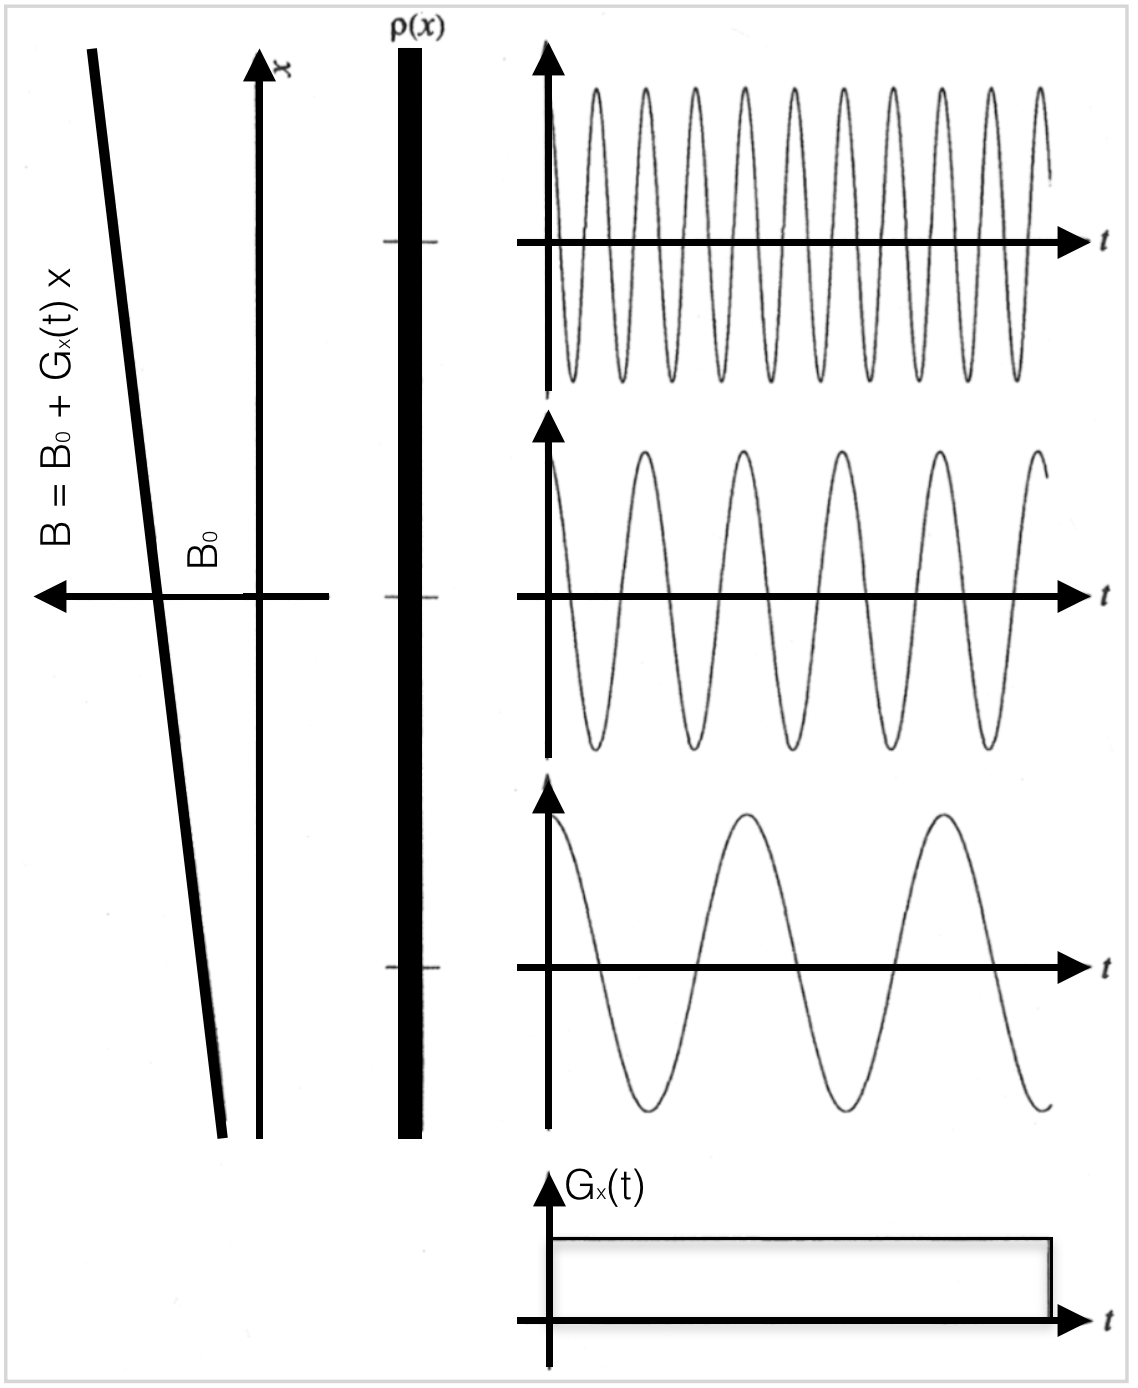
\includegraphics[width=\textwidth]{images/mri/ch10freqenc}
        \caption{Example of how the frequency encoding gradient will affect the signal arising from different locations within a spin system.}
        \label{fig:ch10freqenc}
    \end{subfigure}
    ~ %add desired spacing between images, e. g. ~, \quad, \qquad, \hfill etc. 
      %(or a blank line to force the subfigure onto a new line)
    \begin{subfigure}[b]{0.48\textwidth}
        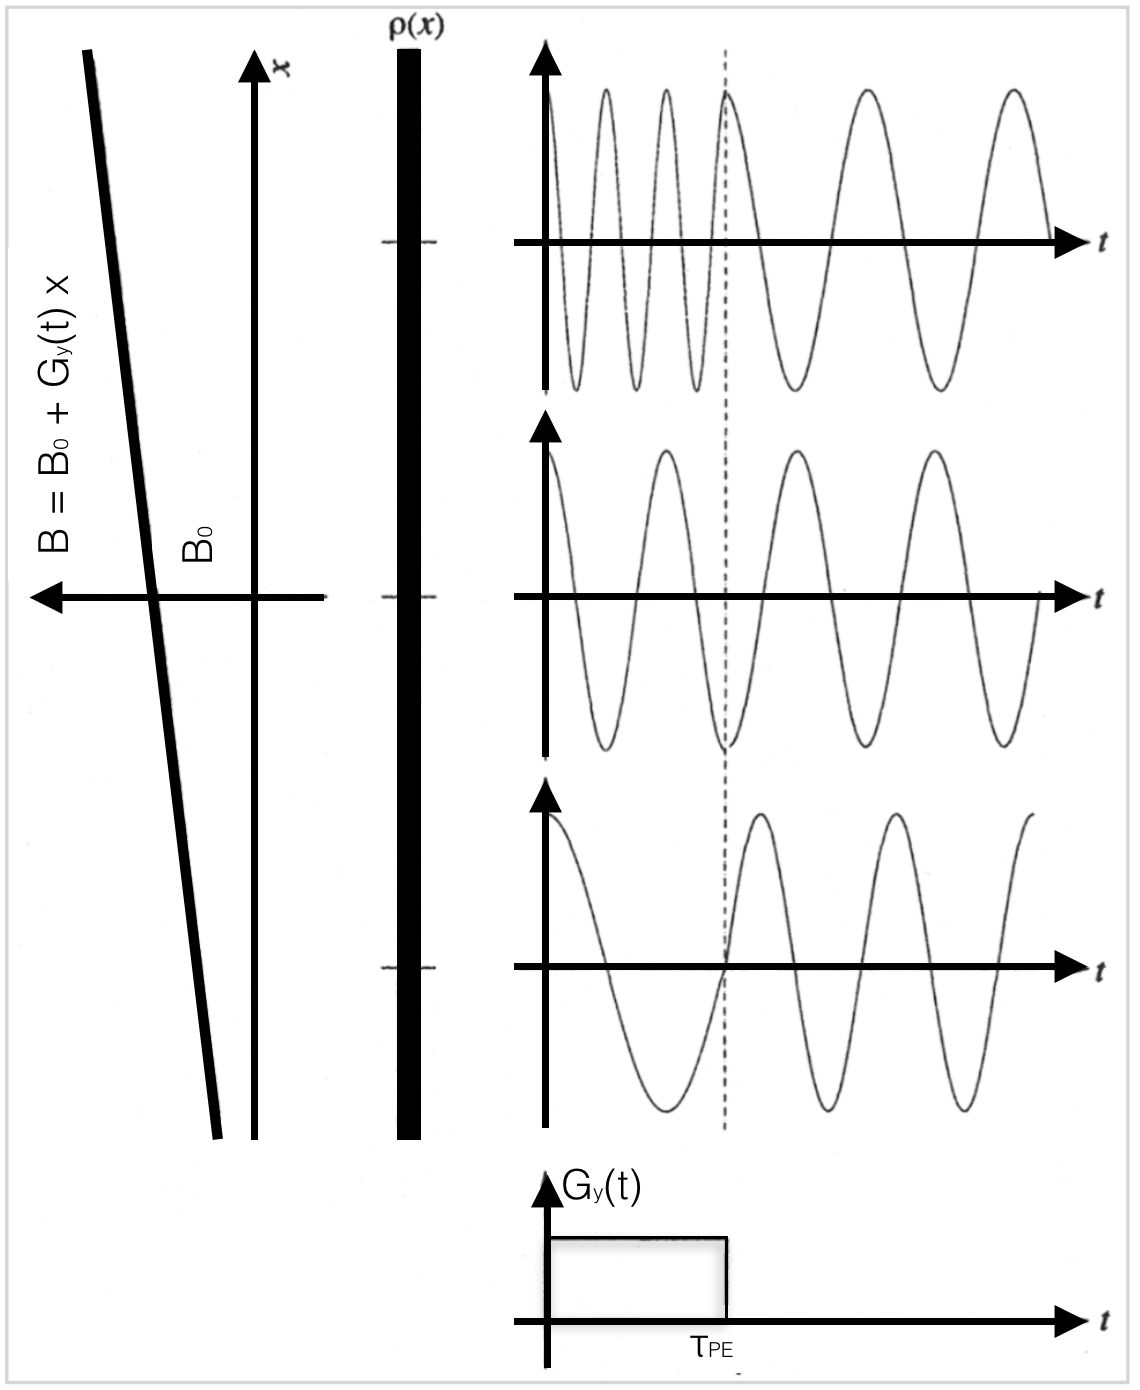
\includegraphics[width=\textwidth]{images/mri/ch10phaseenc}
        \caption{Example of how the phase encoding gradient will affect the signal arising from different locations within a spin system.}
        \label{fig:ch10phaseenc}
    \end{subfigure}
    
    \caption{Frequency encoding and phase encoding are used to spatially localise the signal coming from the sample (Figures adapted from \cite{Liang2000}).}
    \label{fig:ch10freqphaseenc}
\end{figure}

\hfill

% % % % 
\textbf{K-space Representation}
The combination of two perpendicular gradients, one that performs frequency encoding and one that performs phase encoding, leads to the 2D spatial localisation of the slice.
By choosing the slice selection gradient to be in the z-direction, 
only x- and y- gradients are now needed to encode the spatial information in the selected slice.
This information is present in the spatial frequency of the overall detected signal:
\begin{equation}\label{eq:915}
    S(t) = \int \int 
            e^{-t/T_2^*} \rho(x,y) 
                e^{ -i \gamma \int_0^t G_x(t')x + G_y(t')y dt'} dx dy
\end{equation}

By introducing the notion of \textit{spatial frequency} $k = k(t)$ such that:
\begin{equation}\label{eq:kspace}
    k_x(t) = \frac{\gamma}{2 \pi} \int_0^t \vec{G}_x(t') dt' 
    \qquad\text{and}\qquad
    k_y(t) = \frac{\gamma}{2 \pi} \int_0^t \vec{G}_y(t') dt' 
\end{equation}
equation \ref{eq:915} can be rewritten as:
\begin{equation}\label{eq:102}
    S(k_x, k_y) = \int \int e^{-t/T_2^*} \rho(x,y) e^{-i 2 \pi (k_x x + k_y y)} dx dy
\end{equation}

Without taking the relaxation term into account, equation \ref{eq:102} is fundamental to MRI as it is the inverse Fourier transform of the spin density $\rho(x,y)$:
\begin{equation}\label{eq:104}
    \rho(x,y) = \int \int S(k_x,k_y) e^{i 2 \pi (k_x x + k_y y)} dk_x dk_y
\end{equation}

In 2D Cartesian MRI, the signal is collected and stored in a matrix called \textit{k-space} where the axis are the $k_x$ and $k_y$ spatial frequencies. A visual representation of simple 2D Cartesian k-space can be seen in Figure~\ref{fig:ch10kspace}.

\begin{figure}[ht]
    \centering
    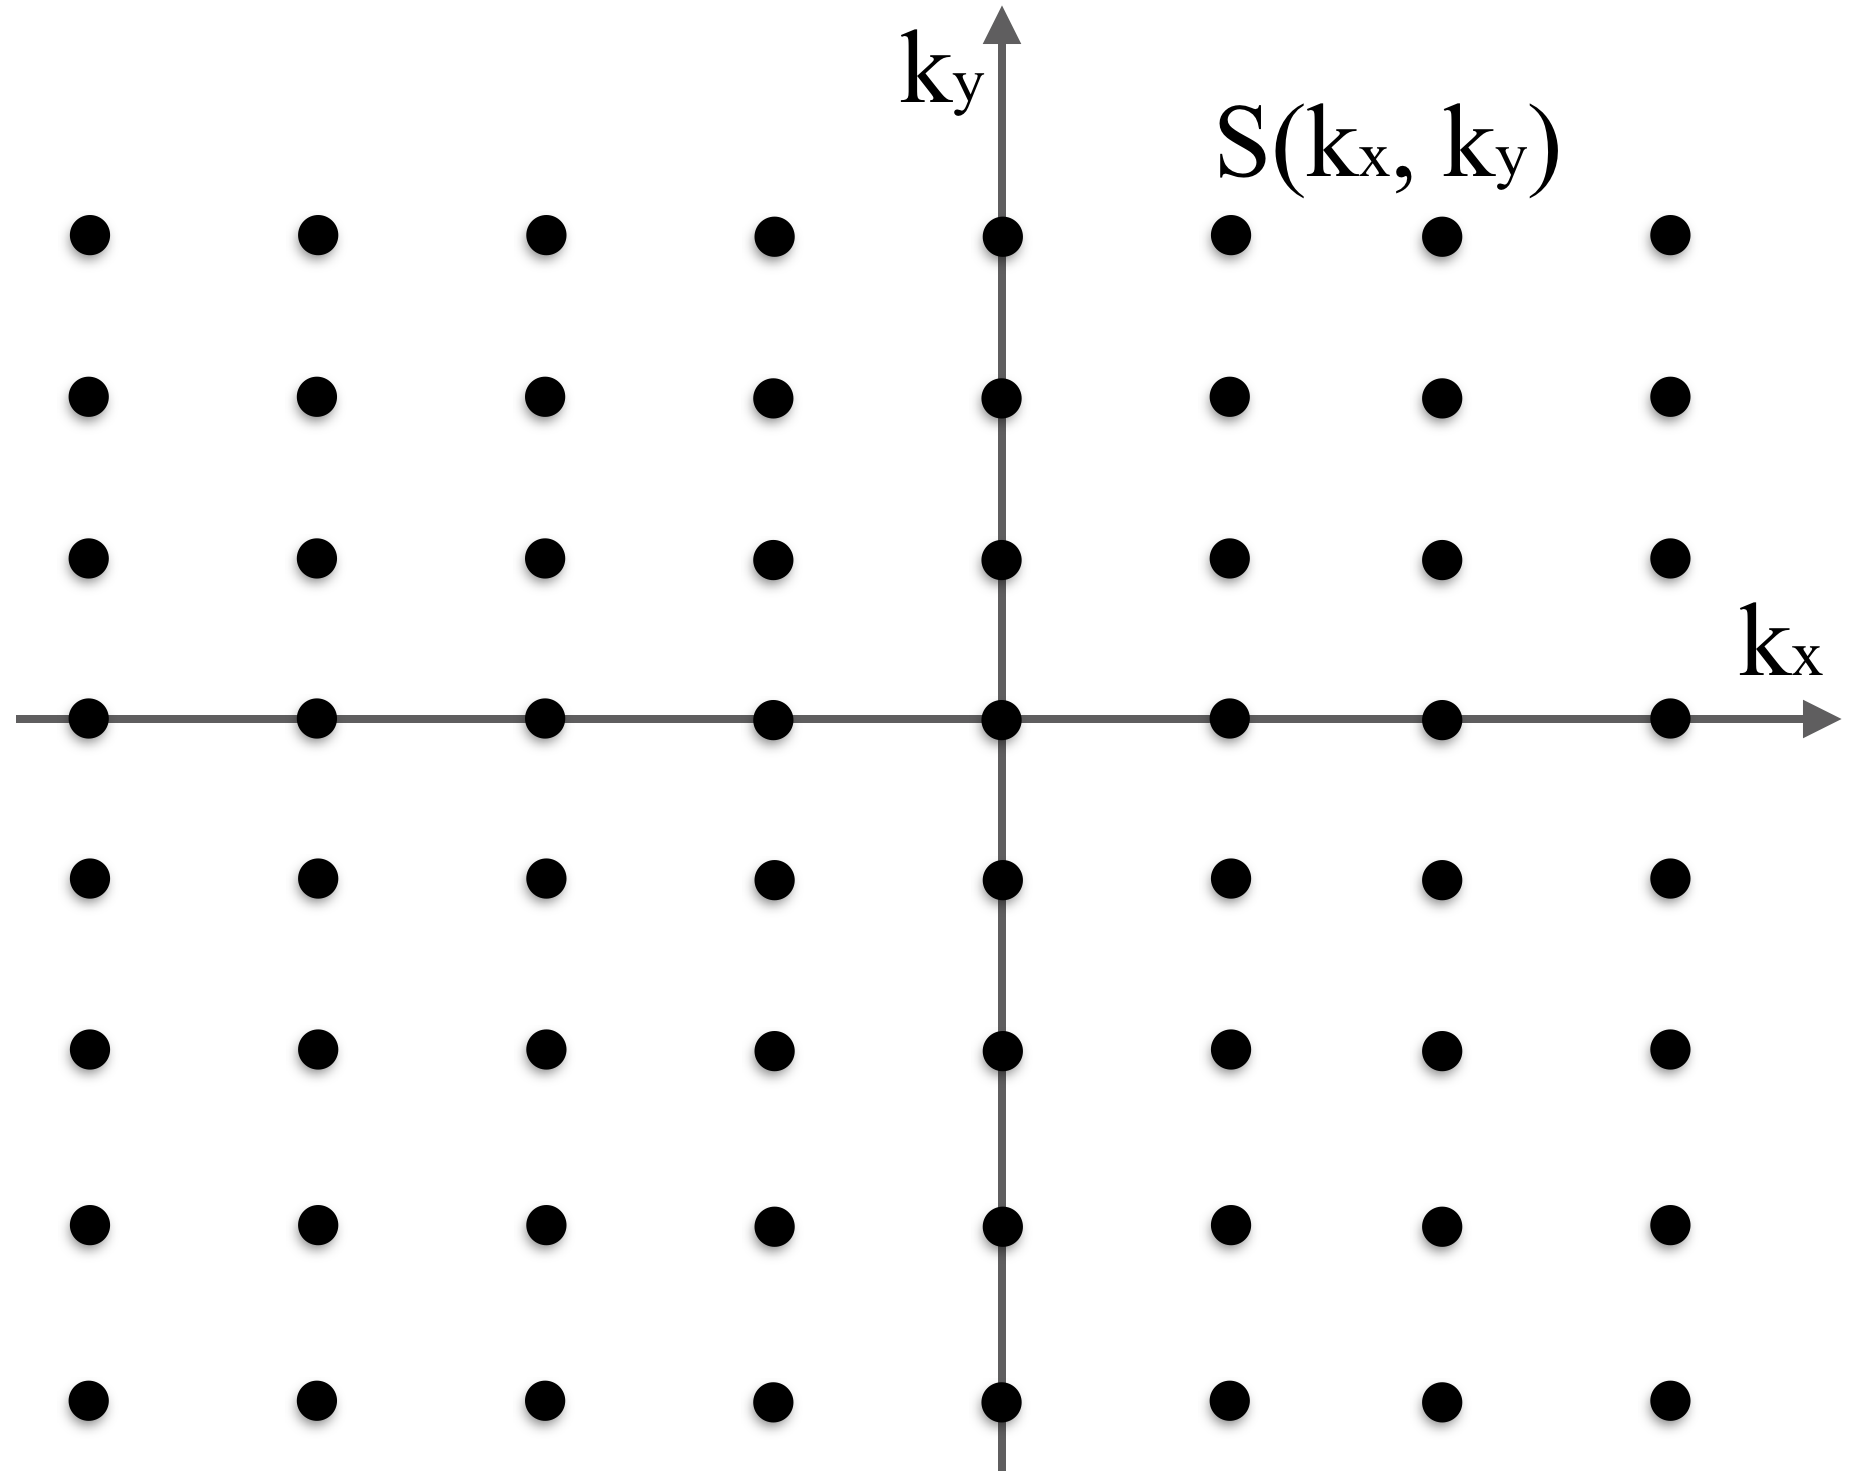
\includegraphics[width=0.5\textwidth,keepaspectratio]{images/mri/ch10kspace}
    \caption{Example of an 8x8 Cartesian k-space. The sampling is asymmetric because it needs to capture the $(k_x, k_y) = (0,0)$ spatial frequencies while keeping an even number of samples in every direction. It is preferred that the number of samples is a power of 2, as the reconstruction method is, in general, a Fast Fourier Transform which works best for those cases.}
    \label{fig:ch10kspace}
\end{figure}

\hfill

% % % % % % % % % % % % 
% % % % % % % % % % % % 
\subsection{Echo Formation}

The signal measured in MRI is called an \textit{echo}. 
Echoes form when a dephased collection of spins is refocused by using one or more applied RF pulses or gradients. 
They are important in MRI because they increase the MR signal due to the rephasing of transverse magnetisation.
There are 3 types of echoes and they can all be obtained by different means: 1) by using a refocusing gradient one can obtain a \textit{gradient echo}, 2) by using an $180^o$ refocusing pulse one can obtain a \textit{spin echo}, and 3) by using 3 rf pulses one can obtain \textit{stimulated echoes}.
The last one is, in general, less useful for imaging and most MRI techniques are tuned to remove the occurance of such echoes.

\hfill

\textbf{Gradient echo.} A gradient echo is obtained by inverting the polarity of the gradient which caused the dephasing. 
This type of echo formation cannot recover the loss of magnetisation due to magnetic field inhomogeneities.
As a consequence, the signal collected for this type of echo will therefore be dependent on $T_2^*$. 
An example of a gradient pulse sequence can be seen in Figure~\ref{fig:gradientecho}.

\hfill

\textbf{Spin echo.} Spin echoes are obtained with an $180^o$ RF pulse. 
After an initial $90^o$ excitation pulse, the spins will start to dephase due to spin-spin interactions and inhomogeneities in the main magnetic field.
The application of the second pulse, the $180^o$ refocusing pulse, will reverse the acquired phase.
This leads to the formation of an echo whose amplitude will no longer depend on $T_2^*$, but on $T_2$.
An example of a spin echo pulse sequence of the $90^o - \tau_1 - 180^o - \tau_2 - \text{Spin-Echo}$ (where $\tau_1 = \tau_2 = T_E/2$) can be seen in Figure~\ref{fig:spinecho}.

\begin{figure}[ht]
\centering
\begin{minipage}{.5\textwidth}
  \centering
  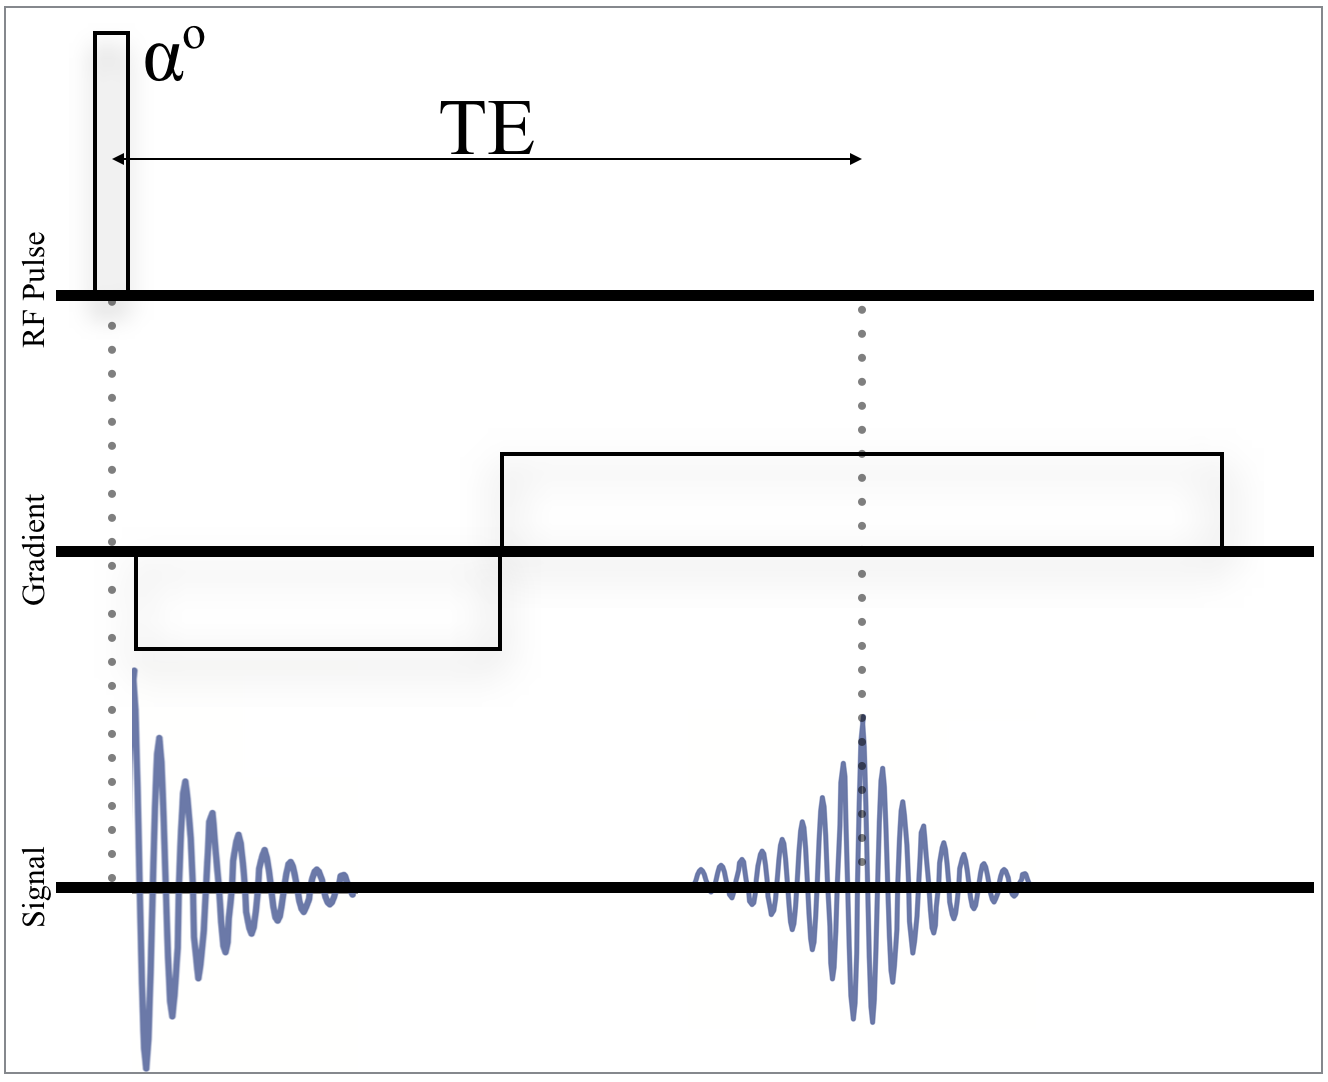
\includegraphics[width=.9\linewidth]{images/mri/gradientecho}
  \captionof{figure}{Example of a gradient echo forming as a result of the application of the second gradient.}
  \label{fig:gradientecho}
\end{minipage}%
\begin{minipage}{.5\textwidth}
  \centering
  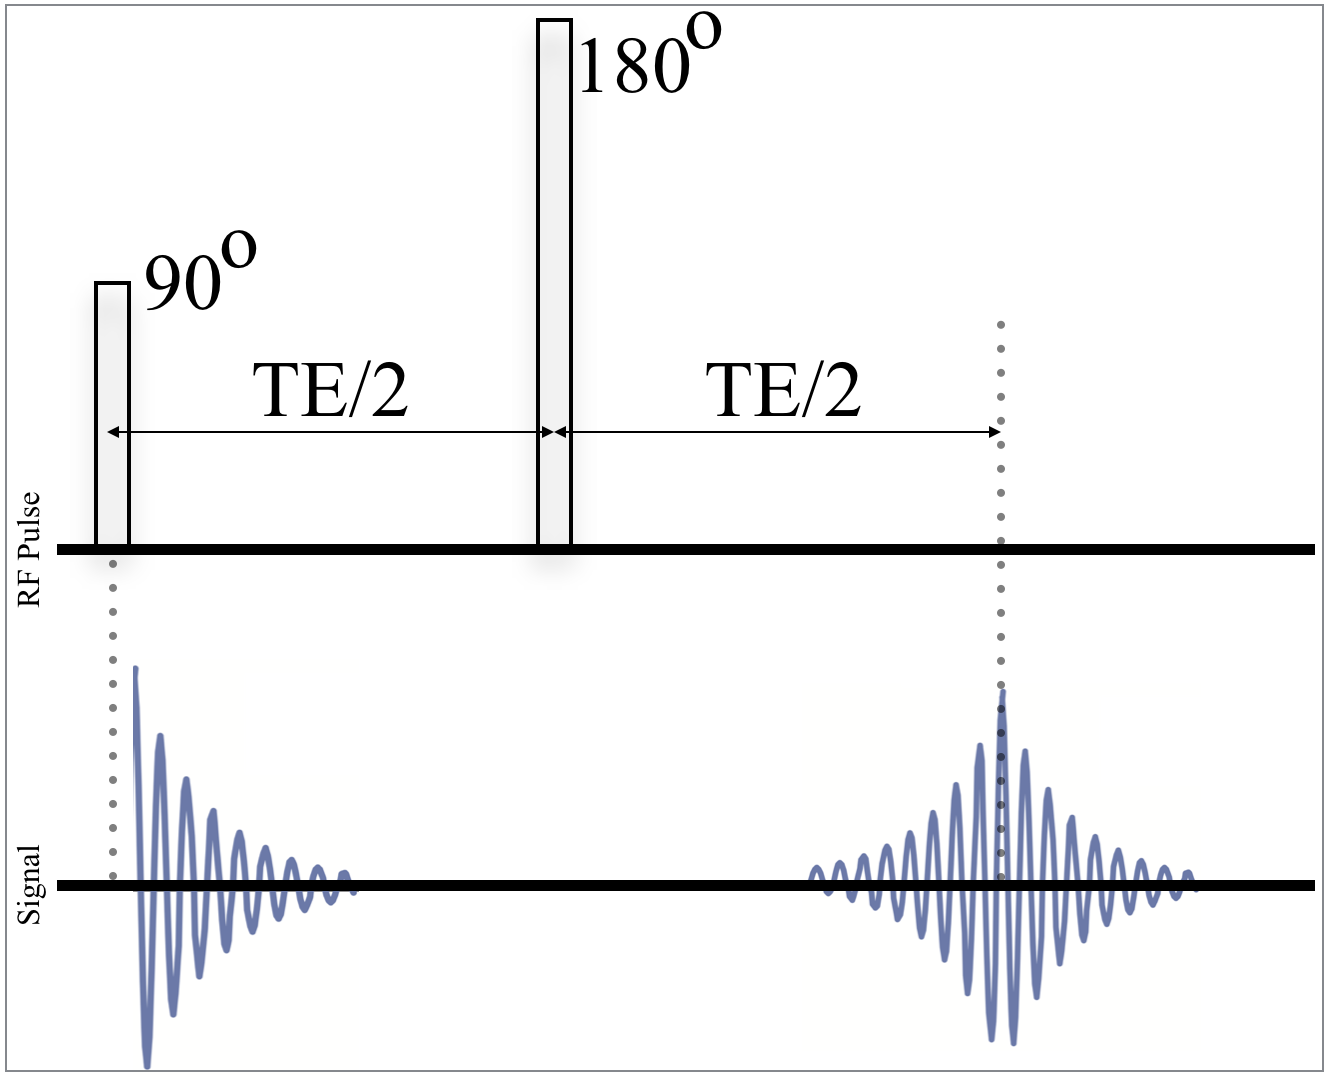
\includegraphics[width=.9\linewidth]{images/mri/spinecho}
  \captionof{figure}{Example of a spin echo forming as a result of the $180^o$ refocusing pulse.}
  \label{fig:spinecho}
\end{minipage}
\end{figure}

\hfill

\textbf{Stimulated echo.} Stimulated echoes are formed after at least 3 RF pulses.
The simplest pulse sequence that gives rise to a stimulated echo is a $90^o - \tau_1 - 90^o - \tau_2 - 90^o - \tau_3 - \text{Stimulated-Echo}$, where $\tau_3 = \tau_1$ is the when the echo forms \cite{Frahm1985}.
Stimulated echoes arise from spins that refocus because of the combination of the three applied RF pulses, together with several other spin echoes \cite{Burstein1996}.
An example of the formation of a stimulated echo is shown in Figure~\ref{fig:stimulatedecho}.

\begin{figure}[ht]
    \centering
    \includegraphics[width=0.95\textwidth,keepaspectratio]{images/mri/stimulatedecho}
    \caption{Example of a stimulated echo forming as a result of 3 $90^o$ RF pulses. The STE forms at $\tau_1$ after the 3rd RF pulse, while the primary SE forms at $\tau_1$ after the 2nd RF pulse. The diagram also shows 3 secondary spin echoes forming after the stimulated echo.}
    \label{fig:stimulatedecho}
\end{figure}

\hfill

% % % % % % % % % % % % % % % 
% % % % % % % % % % % % % % % 
\subsection{Pulse Sequence}

A pulse sequence is a series of magnetic fields used in conjunction with data acquisition to produce MR images.
Pulse sequences are constructed in such a way that they allow the differentiation of tissues by emphasizing in the acquired signal the contribution of the tissue parameters.
In its simplest form, a pulse sequence starts with a $90^o$ excitation pulse applied together with a slice select gradient, to excite the spins found in a certain desired part of the imaged object.
Second, the slice select gradient is followed by an inverse polarity half-area lobe which refocuses the previously dephased spins.
Next, the phase encoding gradient is applied in an orthogonal direction to the slice select gradient, followed by a frequency encoding gradient which will cover the 3rd orthogonal direction.
The frequency encoding gradient is accompanied by data acquisition.
The signal is then demodulated and stored in the spatial frequency matrix called \textit{k-space}.
The final step is then to Fourier transform this matrix and obtain the MR image.

\hfill

% % % % 
\textbf{K-space traversal in 2D Cartesian MRI.}
The pulse sequence used also dictates the way the \textit{k-space} is being filled.
For example, a gradient-echo pulse sequence will fill the matrix line-by-line.
This process can be seen in Figure~\ref{fig:PulseSeqGE}. 
After the slice select gradient is applied, the negative lobe of the phase encoding gradient is played together with the negative lobe of the frequency encoding gradient (step 1).
Next, the signal is acquired while the second (positive) frequency encoding gradient is on (step 2).
This is repeated for different amplitudes of the phase encoding gradient until the entire k-space matrix is filled.

\begin{figure}[ht]
    \centering
    \includegraphics[width=0.95\textwidth,keepaspectratio]{images/mri/PulseSeqGE}
    \caption{Example of a gradient-echo pulse sequence together with the corresponding k-space traversal path.}
    \label{fig:PulseSeqGE}
\end{figure}

The gradient-echo pulse sequence requires a long acquisition time because each line of k-space is acquired separately. 
Echo Planar Imaging (EPI) is a faster method which has been proven to be very useful in a wide variety of MR applications where speed is a requirement.
This method acquires the entire k-space matrix after one excitation pulse (see Figure~\ref{fig:PulseSeqEPI}).
Each line of k-space is traversed either from left to right or from right to left depending on the polarity of the frequency encoding gradient (steps 2 and 4 in the figure).
Moreover, the 'blipped' phase encoding gradients (step 3 in the figure) move the acquisition from one line to the next until the entire matrix is filled.

\begin{figure}[ht]
    \centering
    \includegraphics[width=1\textwidth,keepaspectratio]{images/mri/PulseSeqEPI}
    \caption{Example of a gradient-echo EPI pulse sequence together with the corresponding k-space traversal path.}
    \label{fig:PulseSeqEPI}
\end{figure}

\hfill

% % % % % % % % 
\subsection{Image Reconstruction}

The final step of an MRI acquisition protocol is the reconstruction step.
Once all the spatial information data has been collected, a Fast Fourier Transform (FFT) is used to yield an image (Figure~\ref{fig:fourierReconstruction}). 

\hfill

% % % % 
\textbf{Image Resolution.} The relationship between these two Fourier pairs and the properties of the k-space matrix are of utmost importance in MRI because they dictate the quality and resolution of the final image.
The sampling intervals in both frequency encoding and phase encoding directions in k-space are called $\Delta k_x$ and $\Delta k_y$ and are inversely proportional to the image field-of-view (FOV) \cite{Deshmane2012}:
\begin{equation} \label{eq:1210}
    FOV_x = \frac{1}{\Delta k_x} = \frac{1}{\frac{\gamma}{2 \pi} G_x T_s}
\end{equation}
and
\begin{equation} \label{eq:1211}
    FOV_y = \frac{1}{\Delta k_y} = \frac{1}{\frac{\gamma}{2 \pi} \Delta G_y \tau_y}
\end{equation}

From these relationships we can deduce that an increase in sampling frequency leads to a decrease in the FOV $\Delta k_x \uparrow \, \Rightarrow \, FOV_x \downarrow$ and $\Delta k_y \uparrow \, \Rightarrow \, FOV_y \downarrow$.
Moreover, if we multiply the equations above with $1/N_x$ and $1/N_y$ we see that the highest spatial frequencies sampled in k-space $k_{x,max} = \Delta k_x N_x/2 $ and $k_{y,max} = \Delta k_x N_x/2 $ are inversely proportional to the image resolution $\Delta x$ and $\Delta y$.
We can therefore deduce that an increase in $k_{x,max}$ or $k_{y,max}$ leads to an increase in the image resolution: $k_{x,max} \uparrow \, \Rightarrow \, \Delta x \downarrow$ and $k_{y,max} \uparrow \, \Rightarrow \, \Delta y \downarrow$. 
These findings are summarized in the equations below and in Figure~\ref{fig:fourierReconstruction}.

\begin{equation} \label{eq:1212}
    \Delta x = \frac{1}{N_x \Delta k_x} = \frac{1}{2 k_{x,max}} = \frac{1}{\frac{\gamma}{2 \pi} G_x T}
\end{equation}
and
\begin{equation} \label{eq:1213}
    \Delta y = \frac{1}{N_y \Delta k_y} = \frac{1}{2 k_{y,max}} = \frac{1}{\frac{\gamma}{2 \pi} 2 G_{y,max} t_y}
\end{equation}

\begin{figure}[ht]
    \centering
    \includegraphics[width=1\textwidth,keepaspectratio]{images/mri/fourierReconstruction}
    \caption{The k-space data and the MR image are Fourier pairs. A 2D Fast Fourier Transform applied on the k-space matrix yields the final image. Properties of the sampling and image resolution are presented briefly.}
    \label{fig:fourierReconstruction}
\end{figure}


\hfill

% % % % 
\textbf{Aliasing.} However, if the sampling rate is not high enough such that the \textit{Nyquist-Shannon} theorem is broken, the final image will suffer from aliasing Artifacts \cite{Deshmane2012}. 
Figure~\ref{fig:fourierReconstructionPartial} shows what happens when undersampling occurs in the phase-encoding direction.

\begin{figure}[ht]
    \centering
    \includegraphics[width=1\textwidth,keepaspectratio]{images/mri/fourierReconstructionPartial}
    \caption{Example of different sampling schemes: a) a fully sampled k-space and the final image, b) an acquisition scheme where every other line of k-space in the phase encoding direction has been skipped; this results in aliasing in the same direction, c) only the low spatial frequencies are kept which results in a blurred image}
    \label{fig:fourierReconstructionPartial}
\end{figure}

\hfill

% % % % % % % % % % % % 
% % % % % % % % % % % % 
\subsection{Image Artifacts}

Image artifacts are defined as false features in the final reconstructed image \cite{Haacke1999}. 
They appear as a consequence of the interaction between the imaging protocol and the object under investigation, as well as from the reconstruction process. 
MR image artifacts come in two flavours, each of which can be further categorised depending on the underlying cause:

\hfill

\textbf{Technique-related artifacts}
    \begin{itemize}
        \item \textit{Aliasing} is a frequently encountered MRI artifact. 
        As presented before (see Figure~\ref{fig:fourierReconstructionPartial} b)), aliasing can occur in any direction where the signal has not been sampled densely enough to be reconstructed with high fidelity.
        More specifically, aliasing happens as a consequence of the \textit{analog-to-digital} conversion step, where the otherwise continuous signal is being digitized (sampled).
        The signal digitization is equivalent to the multiplication with a `comb' function which, when Fourier transformed, leads to the periodicity of the object.
        Aliasing can be corrected by increasing the sampling rate in the direction where the artifact occurred, or by using more advanced reconstruction methods such as parallel imaging.
        
        \item \textit{Gibbs Ringing} also appear as a consequence of the \textit{analog-to-digital} conversion step.
        However, unlike aliasing where the problem arises due to digitization, ringing results from windowing the data.
        This signal `truncation' directly translates into sampling the data at a finite number of frequencies.
        This results in an oscillating undershoot and overshoot close to step discontinuities.
        In the final images this appears as multiple parallel lines near interfaces with high-contrast.
        
    \end{itemize}

\hfill

\textbf{Tissue-related artifacts}
    \begin{itemize}
        \item \textit{Chemical Shift} refers to the change in resonant frequency of spins due to the interaction with their local molecular environment.
        For example, fat protons experience a slightly lower magnetic field than a neighbouring water proton because they are shielded by their own electron cloud.
        The difference in frequencies is very small, but increases with higher fields magnets ($215$Hz at $1.5$T and $430$Hz at $3$T).
        As a consequence, when both fat and water protons are found in the same voxel during the frequency-encoding part of the sequence, fat protons will be spatially mapped towards the weaker side of the gradient due to their lower precessing frequency.
        This will cause the appearance of a \textit{shift} along the FE direction in the final image. 
        
        \item \textit{Susceptibility} artifacts refer to a wide variety of MR artifacts that are caused by local magnetic field inhomogeneities.
        In MRI, they are generally encountered near metal implants or at air-tissue and air-bone interfaces where the otherwise homogeneous external magnetic field is locally altered.
        There are three ways the final image is affected:
        \begin{enumerate}
            \item Tissue can be mismapped to a different slice due to being incorrectly excited.
            \item Changes in the tissue frequency can cause geometric distortions.
            \item Signal loss can occur due to accelerated transverse relaxation.
        \end{enumerate}
        
        \item \textit{Motion} is ubiquitous in MRI because
        the time required for the majority of MR sequences to collect the necessary data is much longer than most types of physiological motion, including respiratory motion, vessel pulsation, CSF flow and even involuntary patient motion.
        At best, bulk motion can lead to slice misalignment which can be corrected for with registration algorithms.
        However, if motion happens during the acquisition part of the experiment, it can lead to blurring of object edges, ghosting, loss of information or undesired strong signals \cite{Zaitsev2015}.
        It is therefore important to understand how different types of motion affect the final image in order to correct for the unwanted artifacts, either with motion-correction algorithms, or with better imaging techniques.
        
    \end{itemize}

\hfill 

% % % % % % % % % % % % % % % % 
\section{Fast Imaging Using Non-Cartesian K-space Trajectories}\label{chapterlabel2sec13}

The length of an MRI scan is generally longer compared to other medical imaging modalities such as computer tomography (CT).
It is therefore important to achieve high imaging speeds in MRI in order to make it more clinically feasible \cite{Cohen1991}.
However, imaging speed is limited by the physical constraints of the scanner, such as the amplitude and slew rate of the gradients, and by the physiological constraints of the tissue, such as specific absorption rate (SAR) or peripheral nerve stimulation (PNS).

\hfill

One way to reduce scan time is to acquire less k-space data.
Unfortunately, as we have seen before, this leads to aliasing artifacts in the final images \cite{Pusey1988}.
Despite this, the MR literature presents methods to mitigate these artifacts while maintaining the quality of the final images.
Some of these methods exploit the information provided by the receiver coils and fall under the umbrella of parallel imaging techniques \cite{Griswold2002} \cite{Pruessmann2001} \cite{Pruessmann1999} \cite{Seiberlich2008}, 
others exploit the spatial or temporal redundancy of the k-space data \cite{Tsao2012} \cite{Jung2009} \cite{Tsao2003},
while others benefit from the advent of Compressed Sensing in the signal processing world by exploiting sparsity in the transform domain \cite{Lustig2007} \cite{Pedersen2009} or by using incoherent sampling techniques \cite{Candes2006} \cite{Haldar2011}.

\hfill

% % % % % % % % % % % % 
% % % % % % % % % % % % 
\subsection{Non-Cartesian trajectories}

Other fast imaging techniques include the use of non-Cartesian trajectories.
Based on the properties of the trajectories, these sampling schemes can have many advantages over the conventional Cartesian techniques.
One advantage is that these trajectories can be designed to efficiently use the MR gradient hardware in such a way that it leads to a more rapid coverage of k-space \cite{Wright2014}.

\begin{figure}[ht]
    \centering
    \includegraphics[width=1\textwidth,keepaspectratio]{images/mri/noncarttraj}
    \caption{Example of three different non-Cartesian sampling techniques: a) radial trajectory, b) PROPELLER trajectory and c) spiral trajectory}
    \label{fig:noncarttraj}
\end{figure}

Although there are many non-Cartesian trajectories in the literature, the most popular ones can be seen in Figure~\ref{fig:noncarttraj}.
\textbf{Radial trajectories} (Figure~\ref{fig:noncarttraj} a) are commonly used in 
real-time cardiac imaging because they have the advantage of achieving high temporal resolution by using short echo times \cite{Seiberlich2011} \cite{Schaeffter2001}.
Moreover, due to the inherent oversampling of the center of k-space, radial techniques are known to be more robust to motion or flow artifacts \cite{Pauly1992}.
The \textbf{PROPELER} (Periodically Rotated Overlapping ParallEL Lines with Enhanced Reconstruction) trajectory (Figure~\ref{fig:noncarttraj} b) combines Cartesian and radial sampling in one scheme by simultaneously acquiring a few parallel spokes called `blades'. 
Due to the overlapping central parts, PROPELLER trajectories are commonly used for motion correction \cite{Pipe1999}.
Finally, another common non-Cartesian sampling technique involves \textbf{spiral trajectories} (Figure~\ref{fig:noncarttraj} c). 
These techniques offer a high flexibility in design as spiral trajectories can be constructed to sample k-space either with a constant density pattern \cite{Ahn1986} \cite{Meyer1992} or a variable density pattern \cite{Tsai2000}.
Spiral trajectories are used to reduce motion artifacts in cine cardiac imaging \cite{Kressler2007} and to improve temporal resolution in perfusion imaging \cite{Lee2003}.

\hfill

% % % % % % % % % % % % 
% % % % % % % % % % % % 
\subsection{Gridding}
\label{MRIgridding}

Unlike evenly spaced, uniformly sampled Cartesian k-space data, non-Cartesian trajectories require more complicated algorithms than a simple FFT.
A direct extension of the discrete Fourier Transform for nonrectiliniar data is too computationally slow and therefore impractical.
The alternative is to resample the data onto a Cartesian grid and then apply the FFT.
There are several approaches to this, but the most commonly used one is called `gridding'.

\begin{figure}[ht]
    \centering
    \includegraphics[width=0.7\textwidth,keepaspectratio]{images/mri/gridding}
    \caption{The non-uniformly sampled k-space data points (shown in green) are interpolated onto a Cartesian grid (shown in black). Each sample is convolved with a dedicated kernel (shown in red) and the result is resampled onto the appropriate Cartesian k-space locations.}
    \label{fig:gridding}
\end{figure}

Gridding is a convolution-based reconstruction method that has become popular in MR imaging because it gives good quality results while being faster than most other methods.
This technique relies on estimating a uniformly sampled Cartesian k-space from a non-rectiliniar one (see Figure~\ref{fig:gridding}).
The gridding algorithm is made up of a few steps.
First, if the k-space data has been measured at variable density, each value in the dataset $\big( S(k_i) \big)$ is multiplied with a density correction function $\big( DCF(k_i) \big)$ before interpolation.
Second, each corrected data point ($S'(k_i)$) is convolved with a dedicated kernel $\big( C(k)$ gridding kernel$\big)$ and then resampled onto a Cartesian grid $\big( \Sh (k_j)\big)$. 
These two steps are summarised in the following equations:

\begin{equation}\label{eq:gridding1}
        S'(k_i) = S(k_i) DCF(k_i)
\end{equation}
\begin{equation}\label{eq:gridding2}
        S''(k_j) = [S'(k_i) * C(k)] \Sh (k_j)
\end{equation}

To yield an image, an inverse Fourier transform is applied to the now uniformly sampled k-space data $\big( S''(k_j)\big)$. The convolution with the gridding kernel will lead to a multiplication by the inverse Fourier transform of the kernel $\big( c(\rho_j)\big)$:
\begin{equation}\label{eq:gridding3}
        I''(\rho_j) = \mathcal{F}^{-1} \{ S''(k_j) \} = I(\rho_j) c(\rho_j) \text{ where } c(\rho) = \mathcal{F}^{-1} \{ C(k) \}
\end{equation}

It is therefore important to choose an appropriate kernel function that will not alter the final image.
O'Sullivan found that the best gridding kernel to use would be an infinite sinc function because its transform is rectangular and band-limited \cite{OSullivan1985}.
However, this is not computationally feasible and a compact support function is used instead. 
A finite kernel leads to intensity variation in the image and requires a post-processing step.
This step is called `deapodization' and it involves dividing the reconstructed image by the inverse Fourier transform of the kernel:
\begin{equation}\label{eq:gridding4}
        I(\rho_j) = I''(\rho_j) / c(\rho_j)
\end{equation}

The choice of convolution function is not straightforward.
Jackson et al. \cite{Jackson1991} have conducted a comparative study regarding different filter functions used as gridding kernels.
The conclusion they have reached shows that the Kaiser-Bessel function performs best as the final image is closest to the ideal 'sinc' interpolation.
The Kaiser-Bessel window is therefore the most commonly used kernel in gridding reconstructions.

% % % % % % % % % % % % % % % % 
\section{Fast Imaging Using Steady State Sequences}\label{chapterlabel2sec14}

One other popular way to reduce scan time is to use short repetition times ($T_R$).
$T_R$ is the time from the application of one RF pulse to the application of the next one.
In conventional MRI, repetition times are long enough to allow for full recovery of the longitudinal magnetisation (generally $\geq 5 T_1$) such that at the beginning of the next $T_R$ period the system starts from equilibrium.

\hfill

In 1958, Carr et al \cite{Carr1958} observed that when a spin system is repeatedly excited by a train of equally spaced RF pulses the signal will eventually reach a steady-state.
As the repetition times become shorter, such that they are smaller than the longitudinal relaxation times of the system ($T_R \leq T_1$), the steady-state signal will depend on $T_1$ and $T_R$.
If scan time needs to be reduced even further such that $T_R \leq T_2$, both longitudinal and transverse relaxation are incomplete by the end of the $T_R$ block and the steady-state signal becomes a complicated function of many factors \cite{Hargreaves2012}.

\hfill

Steady-state sequences come in three different flavours, depending on how the residual magnetisation is treated after the imaging portion of the sequence.
These types can be summarised as follows:
\begin{enumerate}
    \item \textit{Steady-state sequences that recover the transverse magnetisation} use balanced gradients, i.e. all the gradients have zero zeroth moment over each repetition time.
    
    \item \textit{Steady-state sequences which average out the transverse magnetisation across a voxel} use `spoiler' gradients at the end of each $T_R$ block.
    
    \item \textit{Steady-state sequences that eliminate the transverse magnetisation} use `spoiler' gradients and vary the phase of each RF pulse.
\end{enumerate}

In the following sections the focus will be on further reviewing two of the most widely used steady-state sequences, the balanced steady-state free precession sequence (bSSFP) and the fast imaging with steady state precession sequence (FISP).

\hfill

% % % % % % % % % % % % 
% % % % % % % % % % % % 
\subsection{bSSFP}
\label{MRIBSSFP}

The balanced steady-state free precession sequence recovers the transverse magnetisation at the end of each $T_R$ period by using balanced (fully rewound) gradients in all directions.
An example of such a sequence can be seen in Figure~\ref{fig:bssfp}.

\begin{figure}[ht]
    \centering
    \includegraphics[width=1\textwidth,keepaspectratio]{images/mri/bssfp2}
    \caption{Example of a balanced steady state free precession sequence (bSSFP). 
    In this type of sequence all gradients on all directions have a net moment of zero at the end of each repetition period.}
    \label{fig:bssfp}
\end{figure}

To better understand the magnetisation dynamics in a sequence with constant $T_R$ and repeated RF pulses of flip angle $\alpha$ and phase angle $\phi = 0$, let us first define a spin ensemble with equilibrium magnetisation $M_0$ and with relaxation constants $T_1$ and $T_2$.
At any time $t$ during the sequence, the magnetisation vector can be described as $M(t) \equiv (M_x(t), M_y(t), M_z(t))$.
In between two consecutive RF pulses the magnetisation vector will relax.
Moreover, if there are any spatially invariant static field inhomogeneities $\Delta B$ present,
the phase of the spins will change over a given repetition time period.
This phase will be determined by $\beta(t) = \Delta \omega t = \gamma \Delta B t$, which becomes $\beta(T_R) = \gamma \, \Delta B \, T_R$ at the end of the repetition time.
By defining the magnetisation vector prior to the $n^{th}$ RF pulse as: $M^-(n) \equiv (M_x^-(n), M_y^-(n), M_z^-(n))$ and the magnetisation vector immediately after the $n^{th}$ RF pulse as: $M^+(n) \equiv (M_x^+(n), M_y^+(n), M_z^+(n))$, we are now in a position to describe the dynamics of the total magnetisation in this sequence.

\hfill

At the end of the $n^{th}$ repetition period, immediately before the $(n+1)^{th}$ RF pulse, the magnetisation vector can be written as:
\begin{equation}\label{eq:ssfp}
    M^-(n+1) = R_z(\beta) D(T_R) R_x(\alpha) M^-(n) + C(T_R)
\end{equation}
where the rotation matrices $R_z$ and $R_x$ and the relaxation matrices $D$ and $C$ have been previously described.

\hfill

When the system reaches steady-state the magnetisation vectors can be set to: $M^-(n+1) = M^-(n)$ and $M^+(n) = M^+(n-1)$. 
As $n$ approaches $\infty$, the solutions to equation \ref{eq:ssfp} are (the details of which can be found in \cite{Haacke1999} and \cite{Dharmakumar2005}):
\begin{equation}
    \begin{split}
        M_x^- (\infty) &= M_0 (1-E_1) \frac{E_2 \, sin \alpha  \, sin \beta}{d} \\
        M_y^- (\infty) &= M_0 (1-E_1) \frac{E_2  \, sin \alpha \,  (cos \beta - E_2)}{d} \\
        M_z^- (\infty) &= M_0 (1-E_1) \frac{[(1 - E_2  \, cos \beta) - E_2  \, cos \alpha  \, (cos \beta - E_2)]}{d} 
    \end{split}
\end{equation}
and
\begin{equation}
    \begin{split}
        M_x^+ (\infty) &= M_x^- (\infty) \\
        M_y^+ (\infty) &= M_0 (1-E_1) \frac{sin \alpha  \, (1 - cos \beta  \, E_2)}{d} \\
        M_z^+ (\infty) &= M_0 (1-E_1) \frac{[E_2 (E_2 - cos\beta) + (1-E_2  \, cos\beta)  \, cos \alpha]}{d} 
    \end{split}
\end{equation}
where $E_1 \equiv e^{-T_R/T_1}$, $E_2 \equiv e^{-T_R/T_2}$ and 
$d = (1-E_1 cos \alpha) (1 - E_2 cos\beta) - E_2 (E_1 cos\alpha) (E_2 - cos \beta)$.

\hfill

It is evident from the above equations that the signal in bSSFP is a complicated function of RF flip angle, $T_1$ and $T_2$ relaxation times and the resonance offset angle.
From the dependence on the $\beta$ angle we can also conclude that inhomogeneities in the main magnetic field will change the signal.
Indeed, different off-resonance angles affect the signal differently and this is summarised in Figure~\ref{fig:sssignal} for two different RF pulse angles.

\begin{figure}[ht]
    \centering
    \begin{subfigure}[b]{1\textwidth}
        \includegraphics[width=\textwidth]{images/mri/ssFA10}
    \end{subfigure}
    
    \begin{subfigure}[b]{1\textwidth}
        \includegraphics[width=\textwidth]{images/mri/ssFA70}
    \end{subfigure}
    
    \caption{Plot of the magnitude of the signal after reaching steady-state for $T_R = 10ms$ and $T_E = 5ms$ for different tissue types and for a) RF pulse flip angle $\alpha = 10^o$ and b) RF pulse flip angle $\alpha = 70^o$}
    \label{fig:sssignal}
\end{figure}

In spite of its high sensitivity to $B_0$ inhomogeneities which causes `banding artifacts' to appear in the final reconstrcted images, bSSFP-type sequences are used clinically today and are known commercially as: True-FISP, FIESTA, Balanced-FFE or True SSFP \cite{Hargreaves2012}.
These sequences yield the highest signal among all the other rapid gradient-echo sequences and give a contrast of $T_2/T_1$ \cite{Scheffler2003}.
Moreover, bSSFP sequences have been used for quantitative imaging \cite{Schmitt2004b} \cite{Gloor2008} and, more recently, in magnetic resonance fingerpriting \cite{Ma2013}.

\hfill

% % % % % % % % % % % % 
% % % % % % % % % % % % 
\subsection{FISP}
\label{MRIFISP}

A different flavour of a steady-state sequence uses gradient `spoilers' at the end of each $T_R$ block.
This type of sequence is known in the literature as a fast imaging with steady state precession (FISP) sequence.
A typical FISP sequence is shown in Figure~\ref{fig:fisp}.
Unlike bSSFP, the precession of each individual spin during each repetition time is now induced by the spoiler gradients who are strong enough to dominate over inhomogenenties.
In fact, gradient spoilers are constructed in such a way that they achieve an integer number of $\pi$ dephasing across a voxel.
This leads to a slight signal loss because the signal arising from one voxel is now an average over the bSSFP signal.

\begin{figure}[ht]
    \centering
    \includegraphics[width=1\textwidth,keepaspectratio]{images/mri/fisp}
    \caption{Example of a fast imaging with steady state precession sequence (FISP). 
    In this type of sequence gradient spoilers are added to one or more axis in each repetition period.}
    \label{fig:fisp}
\end{figure}

The aim of these types of sequences is to avoid the banding artifacts present in bSSFP.
Gradient spoilers can be added to any axis of the sequence or a combination of axis, but it is more common that they are found on the slice selection axis.
While the signal is lower than in bSSFP, it is still a function of $T_2/T_1$ .
Commercially, FISP-type sequences are known as: FE, FFE, GRASS, GRE, FISP, FAST \cite{Hargreaves2012}.
As with bSSFP, the FISP sequence was used by Jiang et al. \cite{Jiang2015} in magnetic resonance fingerprinting to quantify the $T_1$ and $T_2$ relaxation times of the tissue.
 

% % % % % % % % 
% % % % % % % % MRF background
% % % % % % % % 
\chapter{Magnetic Resonance Fingerprinting}
\label{appendixlabelBackgroundMRF}

This chapter gives a concise introduction to the relevant background in Magnetic Resonance Fingerprinting and its current applications. 
It begins with an overview of existing quantitative MR techniques with a particular emphasis on $T_1$ and $T_2$ relaxation times and introduces the general MRF framework.
%along with some of its current applications.

\hfill

% % % % % % % % % % % % % % % % 
\section{Quantitative MRI}\label{chapterlabel2sec21}
Quantitative Imaging is an image acquisition and processing technique whose main objective is to attach a scientific-grade measurement to every pixel in the image such that it can be interpreted independently of the scanner, session, or patient. 
In the medical sciences, quantitative imaging has always been a long-standing goal as it can potentially provide less variability in interpretation, and a higher level of objective evaluation.
However, not all medical imaging techniques are quantitative. 
Conventional MRI, for example, relies on the acquisition of `weighted images', where the image contrast is dependent on both the experiment specifics and tissue properties. 

\hfill

Quantitative Magnetic Resonance Imaging aims to overcome these limitations by providing specific measures of the underlying tissue properties. 
These can include a wide variety of measures such as the proton density of tissue, metabolite concentrations, macromolecular proton fractions, diffusion of water molecules, and others.
However, a large body of research is dedicated to quantifying the $T_1$ and $T_2$ relaxation times of the underlying tissue. 
These metrics have raised a significant interest in the MR community as it was observed that $T_1$ and $T_2$ measures can identify cancerous cells \cite{Damadian1151}, iron accumulation in patients with Parkinson's Disease \cite{JosefVymazal1999}, and inflammation or neural tissue degeneration in multiple sclerosis \cite{MillerD1998}.

\hfill

One drawback of quantitative MRI is that it has a lengthier scan time than conventional MRI. 
For example, $T_1$ and $T_2$ mapping relies on acquiring several images, each with all sequence parameters kept fixed and one specific parameter varied from one acquisition to the next. 
These images are then fitted with a mathematical model in order to estimate the parameters of interest, such as the longitudinal relaxation time $T_1$ \cite{LookLocker1970} or the transverse relaxation time $T_2$ \cite{Giri2009}. 
More recently, other approaches have shortened the acquisition time \cite{Doneva2010} or have provided concurrent measurements of both $T_1$ and $T_2$ \cite{Schmitt2004} relaxation times.
However, these techniques are limited in the number of properties they can retrieve and the accuracy of quantification.

\hfill

To overcome these limitations, a novel quantitative imaging technique called Magnetic Resonance Fingerprinting was developed.
The following section will provide an overview of the MR fingerprinting framework, together with some of its current applications and limitations.

\hfill

% % % % % % % % % % % % % % % % 
\section{The MRF framework}\label{chapterlabel2sec22}

Magnetic resonance fingerprinting (MRF) is a novel quantitative MR imaging method that provides simultaneous measurements of multiple tissue properties in a single acquisition \cite{Ma2013}. 
This technique has recently sparked the interest of many MR scientists and radiologists because it has the potential to detect and analyze early tissue changes, thus improving the information for diagnosis and research in both clinical and preclinical environments. 

\hfill

MRF takes a different approach on performing quantitative MRI than conventional techniques. 
It relies on the assumption that there is a way to construct an MR sequence such that every type of tissue can give rise to unique signal profiles, much like the way our human fingerprints can uniquely identify a person.
In their paper, Ma et al showed that by varying the acquisition parameters in a pseudorandom fashion, the signal can be kept in its transient state.
Moreover, its temporal shape will be different depending on the underlying tissue properties \cite{Ma2013}.

\hfill

\large \textbf{Acquisition Protocol} \normalsize

Every Magnetic Resonance Fingerprinting solution starts with designing the acquisition protocol.
In the original implementation, Ma et al. designed the pulse sequence starting from an inversion recovery balanced steady state free precession (IR-bSSFP) sequence \cite{Ma2013}.
Their decision was based on the knowledge that this type of sequence is known to be sensitive to $T_1$, $T_2$ and off-resonance frequencies \cite{Schmitt2006}.
More recently, a FISP-type sequence was successfully used by Jiang et al. which removes the banding artifacts caused by the bSSFP sequences \cite{Jiang2015}. 
This has now become the most popular form of MRF for $T_1$ and $T_2$ quantification.

\hfill

However, the MRF framework is highly versatile.
The literature to date shows that for different parameters of interest, the pipeline can be adapted to incorporate ideas from other MR sequences.
For example, Jiang et al. \cite{Jiang2017} showed promising results in generating apparent diffusion coefficient (ADC) maps on top of $T_1$ and $T_2$ maps, by incorporating diffusion-preparation modules \cite{Thomas1998} in a FISP-based MRF sequence.
For brain hemodynamics, Su et al. \cite{Su2017} introduced Arterial Spin Labelling (ASL) `label' and `control' modules in the pipeline and created cerebral blood flow (CBF) and bolus arrival time (BAT) maps.
Finally, for cardiac MRI, data was collected only during diastole in a study held by Hamilton et al. \cite{Hamilton2017} and single slice $T_1$ and $T_2$ maps in the heart were generated.

\hfill

After the sequence protocol has been selected, the MRF framework becomes a three stage pipeline which is summarised in Figure~\ref{fig:mrfPipeline} and in the following sections.

% % % % % % % % % % % % % % % % % % % % % % % % 
\hfill

\large\textbf{Data collection} \normalsize

In the data collection step, two types of datasets are constructed.
\begin{itemize}
    % % % % % 
    \item \textbf{Dictionary.} First, signal evolutions are generated for a wide range of tissue properties and then stored in a database called dictionary. 
    For bSSFP-type sequences, Bloch based
    %or Bloch-McConnell 
    simulations are used to generate the signals \cite{Hamilton2015}.
    For FISP-type sequences, where dephasing across a voxel has to be taken into account, a more sophisticated algorithm is used, called the `extended phase graph' formalism \cite{Weigel2015}. 
    
    In terms of tissue properties, most studies consider the $T_1$ and $T_2$ relaxation times \cite{Ma2013} \cite{Jiang2015} \cite{Hamilton2017} \cite{Gao2015} \cite{Amthor2017} \cite{Buonincontri2017}.
    Other applications are interested in more sophisticated properties such as the apparent diffusion coefficient \cite{Jiang2017} or cerebral blood volume, mean vessel radius and oxygenation maps \cite{Christen2014}.
    
    Finally, a few studies have introduced system parameters.
    Cloos et al. \cite{Cloos2016} investigated the usage of multi-transmit coils in an MRF application for titanium hip implants.
    The study introduced alternating $B_1^+$ illumination profiles interwoven in the MRF sequence and coined it as plug-and-play MRF (PnP-MRF), while successfully quantifying the $B_1^+$ non-uniformities together with the desired tissue properties.
    However, this technique requires multi-transmit RF coils with different illumination profiles that are not yet available in every centre.
    For this reason, Buonincontri et al. \cite{Buonincontri2017} introduced abrupt changes in flip angles in the MRF acquisition sequence to estimate the $B_1$ field without using special equipment.
    
    % % % % % 
    \item \textbf{Images.} After the desired application-dependent dictionary has been created, the image acquisition step is performed using the same sequence parameters as in the dictionary creation stage.
    In the original MRF implementation, Ma et al. \cite{Ma2013} used a variable density spiral acquisition which was rotated from one $T_R$ to the next.
    To fully sample k-space, they acquired the same dataset 48 times, each time with a different starting angle of the spiral.
    Although spiral acquisitions are popular among MRF applications, other techniques have also been investigated.
    For example, Cohen et al. \cite{Cohen2016} used fully sampled Cartesian EPI acquisitions, while Cloos et al. \cite{Cloos2016} used radial acquisitions.

\end{itemize}

% % % % % % % % % % % % % % % % % % % % % % % % 
\hfill

\large \textbf{Pattern recognition} \normalsize

After the acquisition, a pattern recognition algorithm is used to retrieve the parameters of interest.
In the original MRF implementations, a vector dot-product was performed between every acquired signal and the dictionary \cite{Ma2013} \cite{Jiang2015}. 
The dictionary signal that gave the highest score was then chosen to be the most representative one for the voxel that was under investigation.
However, this technique can be time consuming for very large dictionaries.
For this reason, more recent studies have looked into ways of speeding up the process.
For example, McGivney et al. \cite{McGivney2014} used SVD compression to reduce the size of the dictionary.
This led to a speed up in the pattern matching step.
Cauley et al. \cite{Cauley2015fgm} divided the dictionary into several groups based on correlations between entry points and performed the matching only on a representative signal of a group, thus finding the best match more quickly.


% % % % % % % % % % % % % % % % % % % % % % % % 
\hfill

\large \textbf{Information retrieval} \normalsize

The final step of the pipeline is the information retrieval step.
This step involves the creation of the quantitative maps.
This is done by repeating the pattern matching process for every voxel in the acquired images and retrieving the tissue parameters that were used to generate the most representative dictionary signal.
This can also be seen in part three of Figure~\ref{fig:mrfPipeline}.

\hfill

Good quality maps require a number of conditions to be achieved.
First, a large enough dictionary must be created to account for a wide range of possible tissue parameter combinations.
Second, for pseudo-random acquisition parameters, a long enough sequence is needed to allow for better discrimination between signals coming from different tissues. 
More recently, Zhao et al. \cite{Zhao2017}, Cohen et al. \cite{Cohen2016} and Sommer et al. \cite{Sommer2017} investigated ways to optimise the sequence for both better encoding capabilities and shorter scan time.
Finally, high quality maps require that the sample does not move.

\hfill

\textbf{Motion.} The motion robustness of this technique has been investigated in the original MRF implementation by Ma et al. \cite{Ma2013} where the volunteer was asked to randomly move his/her head during the last 3s of a 15s scan.
In this case, the authors reported that the final maps were not affected by the movements.
However, a more recent experimental study conducted by Yu et al. \cite{Yu2017} investigated various types of motion occurring at different times during the scan.
Using radial acquisition, their results show that $T_1$ maps become blurry if the motion happens early in the scan, while $T_2$ maps are mostly affected when motion happens in the middle.
However, in experimental studies it is hard to quantify the type and amount of motion the volunteer has performed.
Therefore, one of the aims of my work is to investigate the impact of motion in an MRF experiment in a controlled and reliable manner, which can only be achieved through simulation.

\begin{figure}[ht]
    \centering
    % \makebox[\textwidth][c]{\includegraphics[width=1.4\textwidth]{images/mri/mrfPipeline}}%
    \includegraphics[width=1\textwidth]{images/mri/mrfPipeline}
    \caption{The MRF pipeline: \textbf{(1)} in the first stage images are collected and the dictionary of signals is simulated; \textbf{(2)} in the second stage the pattern recognition algorithm is performed between every acquired signal and the dictionary; the dictionary signal with the highest score is then chosen as the most representative one for that voxel; \textbf{(3)} in the final stage the information associated with each match is retrieved and the quantitative maps are created}
    \label{fig:mrfPipeline}
\end{figure}

 

% % % % % % % % 
% % % % % % % % Phantom Values
% % % % % % % % 
\chapter{$T_1$ and $T_2$ relaxation times of the digital phantom}
\label{appendixlabelPhantom}
% % % % Include Table
\begin{table}[h!]
\centering
 \begin{tabular}{||c c c c ||} 
 \hline
 Index & $T_1$ (ms) & $T_2$ (ms) & $\rho$ \\ [0.5ex] 
 \hline\hline
 0 & 500 & 360 & 1 \\
 \hline
 1 & 225 & 50  & 1  \\ 
 \hline
 2 & 335 & 70  & 1  \\
 \hline
 3 & 330 & 110  & 1  \\
 \hline
 4 & 1010 & 130  & 1  \\
 \hline
 5 & 1615 & 370  & 1 \\ 
 \hline
 6 & 675 & 90  & 1 \\ 
 \hline
 7 & 665 & 130  & 1 \\ 
 \hline
 8 & 840 & 110  & 1 \\ 
 \hline
 9 & 830 & 150  & 1 \\ 
 \hline
 10 & 1150 & 155  & 1 \\ 
 \hline
 11 & 1420 & 190  & 1 \\ 
 \hline
 12 & 1580 & 160  & 1 \\ 
 \hline
\end{tabular}
\caption{$T_1$ and $T_2$ relaxation times of the digital phantom used in the simulations found throughout this thesis. The inner circles are represented with indices ranging from 1 to 12, while the big circle is represented by index 0.}
\label{table:1}
\end{table} 

% % % % % % % % 
% % % % % % % % Motion maps
% % % % % % % % 
\chapter{Motion corrupted quantitative maps}
\label{appendixlabelMotion}
% % % % Motion corrupted Quantitative maps 
% T1 maps motion
\begin{figure}[ht]
    \centering
    \includegraphics[width=1\textwidth]{images/mrf/T1mapsmotion}
    \caption{Motion corrupted $T_1$ quantitative maps for all 9 types of motion traces. First column corresponds to the \textit{motion 1} trace (continuous rotation about the z-axis), the second column corresponds to the \textit{motion 2} trace (continuous translation along the y-axis) and the third column corresponds to the \textit{motion 3} trace (continuous rotation about the z-axis and continuous translation along the y-axis). Different lines correspond to a different onset of motion.}
    \label{fig:appendixT1mapsmotion}
\end{figure}

% T2 maps motion
\begin{figure}[ht]
    \centering
    \includegraphics[width=1\textwidth]{images/mrf/T2mapsmotion}
    \caption{Motion corrupted $T_2$ quantitative maps for all 9 types of motion traces. First column corresponds to the \textit{motion 1} trace (continuous rotation about the z-axis), the second column corresponds to the \textit{motion 2} trace (continuous translation along the y-axis) and the third column corresponds to the \textit{motion 3} trace (continuous rotation about the z-axis and continuous translation along the y-axis). Different lines correspond to a different onset of motion.}
    \label{fig:appendixT2mapsmotion}
\end{figure}

% Score maps motion
\begin{figure}[ht]
    \centering
    \includegraphics[width=1\textwidth]{images/mrf/scoremapsmotion}
    \caption{Motion corrupted matching score maps for all 9 types of motion traces. First column corresponds to the \textit{motion 1} trace (continuous rotation about the z-axis), the second column corresponds to the \textit{motion 2} trace (continuous translation along the y-axis) and the third column corresponds to the \textit{motion 3} trace (continuous rotation about the z-axis and continuous translation along the y-axis). Different lines correspond to a different onset of motion.}
    \label{fig:appendixscoremapsmotion}
\end{figure}

% T1 motion maps zoom
\begin{figure}[ht]
    \centering
    \includegraphics[width=1\textwidth]{images/mrf/T1mapsmotionzoom}
    \caption{Zoomed in $T_1$ maps for different types of motion}
    \label{fig:appendixT1mapsmotionzoom}
\end{figure}

% T2 motion maps zoom
\begin{figure}[ht]
    \centering
    \includegraphics[width=1\textwidth]{images/mrf/T2mapsmotionzoom}
    \caption{Zoomed in $T_2$ maps for different types of motion}
    \label{fig:appendixT2mapsmotionzoom}
\end{figure}

% ROI analysis motion 1
\begin{figure}[ht]
    \makebox[\textwidth][c]{\includegraphics[width=1.4\textwidth]{images/mrf/motion1ROI}}
    \caption{Region of interest analysis on \textit{motion 1} for different motion onsets}
    \label{fig:appendixmotion1ROI}
\end{figure}

% ROI analysis motion 2
\begin{figure}[ht]
    \makebox[\textwidth][c]{\includegraphics[width=1.4\textwidth]{images/mrf/motion2ROI}}
    \caption{Region of interest analysis on \textit{motion 2} for different motion onsets}
    \label{fig:appendixmotion2ROI}
\end{figure}

% ROI analysis motion 3
\begin{figure}[ht]
    \makebox[\textwidth][c]{\includegraphics[width=1.4\textwidth]{images/mrf/motion3ROI}}
    \caption{Region of interest analysis on \textit{motion 3} for different motion onsets}
    \label{fig:appendixmotion3ROI}
\end{figure}

% % % % % % % % 
% % % % % % % % Pseudocode for bSSFP
% % % % % % % % 
\chapter{Pseudocode for Generating the bSSFP Dictionary}
\label{appendixlabel1}
% % % % Create dictionary
\begin{algorithm}
\setstretch{1}
    \LinesNumberedHidden
    \SetKwInOut{Input}{Input}
    \SetKwInOut{Output}{Output}

    \nonl \underline{function createDictionary} ($\bm{matProps, seqProps}$)\;
    \Input{
        $\bm{matProps}$ a (structure) with $\bm{T_1, T_2, \Delta f}$ fields in (ms, ms, kHz) \\
        \hspace*{0.4cm} representing the $T_1$ and $T_2$ relaxation times and the \\
        \hspace*{0.4cm} off-resonance frequency of the entire \\
        \hspace*{0.4cm} set of material properties \\
        $\bm{seqProps}$ a (structure) with $\bm{RF: (FA, PhA), T_R, RO}$ fields \\
        \hspace*{0.4cm} representing the RF pulse, repetition time and \\
        \hspace*{0.4cm} read out time of the entire N-block sequence \\
        \hspace*{0.4cm} where $\bm{RF}$ is a structure with $FA$ and $PhA$ \\
        \hspace*{0.4cm} representing the flip angles and \\
        \hspace*{0.4cm} phase angles of the RF pulses in degrees}
    \Output{$\bm{dictionaryMRF}_{(M \times N \times 3)}$ the $x,y,z$ components of the magnetic moment vector at all N read-out points and for every combination of material properties, where $M = N_{T_1} \times N_{T_2} \times N_{\Delta f}$ is the number of tissue properties}
    
    \nonl \phantom{lala}
    
    %% Step 1
    \texttt{(cD1.) Precompute RF pulse matrices: } 
    \begin{flalign*}
    R_{RF} \gets 
    \begin{bmatrix}
        R_{z}(\phi_1) R_{x}(-\alpha_1) R_{z}(-\phi_1) \\
        R_{z}(\phi_2) R_{x}(-\alpha_2) R_{z}(-\phi_2) \\
                        \dots                         \\
        R_{z}(\phi_N) R_{x}(-\alpha_N) R_{z}(-\phi_N)
    \end{bmatrix}_{(N \times 3 \times 3)}
    \end{flalign*}
    
    %% Step 2
    \texttt{(cD2.) Retrieve set of material properties: } 
    \begin{flalign*}
    \text{\texttt{materialTuples}} & \gets
    \begin{bmatrix}
        T_{1_{ijk}} & T_{1_{ijk}} & \dots & T_{1_{ijk}} \\
        T_{2_{ijk}} & T_{2_{ijk}} & \dots & T_{2_{ijk}} \\
        \Delta f_{ijk} & \Delta f_{ijk} & \dots & \Delta f_{ijk} \\
    \end{bmatrix}_{(3 \times M)} \\
    & \text{ with } i \in [1, N_{T_1}], j \in [1, N_{T_2}], k \in [1, N_{\Delta f}] \text{ (nested looping)}
    \end{flalign*}
    
    \fontsize{8pt}{8pt}\selectfont
    \caption{Function that creates the entire dictionary}
    \label{alg:createDictionary}
\end{algorithm}

\begin{algorithm}
\setstretch{1}
    \LinesNumberedHidden

    %% Step 3
    \nonl \texttt{(cD3.) Initialize magnetic moment vector matrix} \\
    \nonl $\bm{M} \gets repmat([0; 0; 1], [1,M]);$

    %% Step 4
    \nonl \texttt{(cD4.) Go through each TR block} \\
    \nonl \For{$i \in [1, N]$} {
        %% Step 4.1
        \nonl \texttt{(cD4.1.) Create rotation matrices for off-resonance effects}
        \begin{flalign*}
            [R_{offRes1}, beta] &\gets \text{\texttt{createRoffres1(materialTuples, seqProps, i)}} \\
            R_{offRes2} &\gets \text{\texttt{createRoffres2(materialTuples, beta)}} 
        \end{flalign*}
        
        %% Step 4.2
        \nonl \texttt{(cD4.2.) Create relaxation matrices}
        \begin{flalign*}
            [D, D_z] &\gets \text{\texttt{createD(materialTuples, seqProps, i)}}
        \end{flalign*}
        
        %% Step 4.3
        \nonl \texttt{(cD4.3.) Calculate $M_{next}$ and $M_{RO}$ for current TR block}
        \begin{flalign*}
            [\bm{M, M_{RO}}] \gets \text{\texttt{sequenceBlock($\bm{M}, R_{RF}(i), R_{offRes1}, R_{offRes2}, D, D_z$)}}
        \end{flalign*}
        
        %% Step 4.4
        \nonl \texttt{(cD4.4.) Store $M_{RO}$ for current TR block}
        \begin{flalign*}
            dictionaryMRF(i) \gets \bm{M_{RO}}
        \end{flalign*}
    \nonl }

    %% Step 5
    \nonl \texttt{(cD5.) RETURN} $dictionaryMRF$ \;    
    
    \fontsize{8pt}{8pt}\selectfont
\end{algorithm}

 
% % % % Sequence Block
\begin{algorithm}
\setstretch{1}
    \LinesNumberedHidden
    \SetKwInOut{Input}{Input}
    \SetKwInOut{Output}{Output}

    \nonl \underline{function sequenceBlock} $(\bm{M_{prev}, R_{RF}, R_{offRes1}, R_{offRes2}, D, D_z})$\;
    \Input{
    $\bm{M_{prev}}$ a $(3 \times M)$ matrix storing the $x,y,z$ components of the \\
    \hspace*{0.4cm} magnetic moment vector for the entire set of tissue \\
    \hspace*{0.4cm}  properties before the current sequence block, \\
    $\bm{R_{RF}}$ a $(3 \times 3)$ matrix used for flipping the magnetic moment \\
    \hspace*{0.4cm} vector as a result of the application of the RF pulse, \\
    $\bm{R_{offRes1}}$ a $(3 \times M)$ matrix used to simulate off-resonance effects, \\
    $\bm{R_{offRes2}}$ a $(3 \times M)$ matrix used to simulate off-resonance effects, \\
    $\bm{D}$ a $(3 \times M)$ matrix used to simulate relaxation effects and \\
    $\bm{D_z}$ a $(3 \times M)$ matrix used to simulate relaxation effects}
    \Output{$\bm{M_{next}}$ a $(3 \times M)$ matrix storing the $x,y,z$ components of the \\
    \hspace*{0.4cm} magnetic moment vector for the entire set of tissue \\
    \hspace*{0.4cm} properties before the next sequence block}
    
    \phantom{lala}
    
    %% Step 1
    \texttt{(sB1.) Do RF pulse: } 
    $ M_{next_{(3 \times M)}} \gets R_{RF_{(3 \times 3)}} \, M_{prev_{(3 \times M)}} =  
    R_{RF_{(3 \times 3)}}
    \begin{bmatrix}
        x_{1} & x_{2} & \dots & x_{M} \\
        y_{1} & y_{2} & \dots & y_{M} \\
        z_{1} & z_{2} & \dots & z_{M}
    \end{bmatrix}_{(3 \times M)} $ \\
    
    %% Step 2
    \texttt{(sB2.) Do off-resonance: } 
    \begin{flalign*}
    M_{next_{(3 \times M)}} \gets & R_{offRes1_{(3 \times M)}} \, \odot \, M_{next_{(3 \times M)}} + R_{offRes2_{(3 \times M)}} \, \odot \, \text{permuteLines12}(M_{next_{(3 \times M)}}) = \\
    & \begin{bmatrix}
	    \phantom{-}\cos(\beta_{1}) & \phantom{-}\cos(\beta_{2}) & \dots & \phantom{-}\cos(\beta_{M}) \\
        \phantom{-}\cos(\beta_{1}) & \phantom{-}\cos(\beta_{2}) & \dots & \phantom{-}\cos(\beta_{M}) \\
               1                   &        1                   & \dots &        1
    \end{bmatrix}_{(3 \times M)} \odot 
    \begin{bmatrix}
        x_{1} & x_{2} & \dots & x_{M} \\
        y_{1} & y_{2} & \dots & y_{M} \\
        z_{1} & z_{2} & \dots & z_{M}
    \end{bmatrix}_{(3 \times M)}
    + \\
    & \begin{bmatrix}
	    -\sin(\beta_{1})           & -\sin(\beta_{2})           & \dots & -\sin(\beta_{M}) \\
        \phantom{-}\sin(\beta_{1}) & \phantom{-}\sin(\beta_{2}) & \dots & \phantom{-}\sin(\beta_{M}) \\
               0                   &        0                   & \dots &        0
    \end{bmatrix}_{(3 \times M)} \odot 
    \begin{bmatrix}
        y_{1} & y_{2} & \dots & y_{M} \\
        x_{1} & x_{2} & \dots & x_{M} \\
        z_{1} & z_{2} & \dots & z_{M}
    \end{bmatrix}_{(3 \times M)}
    \end{flalign*}
    
    %% Step 3
    \texttt{(sB3.) Do relaxation: } 
    \begin{flalign*}
    M_{next_{(3 \times M)}} & \gets D_{_{(3 \times M)}} \, \odot \, M_{next_{(3 \times M)}} \, + \, D_{z_{(3 \times M)}} \\
    & \begin{bmatrix}
	    E_{2_{1}} & E_{2_{2}} & \dots & E_{2_{M}} \\
        E_{2_{1}} & E_{2_{2}} & \dots & E_{2_{M}} \\
        E_{1_{1}} & E_{1_{2}} & \dots & E_{1_{M}}
    \end{bmatrix}_{(3 \times M)} \odot
    \begin{bmatrix}
        x_{1} & x_{2} & \dots & x_{M} \\
        y_{1} & y_{2} & \dots & y_{M} \\
        z_{1} & z_{2} & \dots & z_{M}
    \end{bmatrix}_{(3 \times M)} + \\
    & \begin{bmatrix}
    	0 & 0 & \dots & 0 \\
        0 & 0 & \dots & 0 \\
        1-E_{1_{1}} & 1-E_{1_{2}} & \dots & 1-E_{1_{M}}
    \end{bmatrix}_{(3 \times M)}
    \end{flalign*}
    
    %% Step 3
    \texttt{(sB4.) RETURN } $M_{next_{(3 \times M)}}$ \;
    
    \caption{Vectorised sequence block function which calculates the magnetisation vector components at the end of a sequence block for the entire set of tissue properties of size \texttt{M}. Note: $\odot$ denotes component-wise multiplication}
    \label{alg:sequenceBlock}
\end{algorithm}


 
% % % % Create off res
\begin{algorithm}
\setstretch{1}
    \LinesNumberedHidden
    \SetKwInOut{Input}{Input}
    \SetKwInOut{Output}{Output}

    \nonl \underline{function createRoffres1} ($\bm{materialTuples, seqProps, seqID}$)\;
    \Input{
        $\bm{materialTuples}$ a ($3 \times M$) matrix with all $\bm{T_1, T_2, \Delta f}$ \\
        \hspace*{0.4cm} combinations for each line \\
        $\bm{seqProps}$ a (structure) with $\bm{RF: (FA, PhA), T_R, RO}$ fields \\
        \hspace*{0.4cm} representing the RF pulse, repetition time and read out time \\
        \hspace*{0.4cm} of the entire N-block sequence where $\bm{RF}$ is a structure with \\
        \hspace*{0.4cm} $FA$ and $PhA$ representing the flip angles and \\
        \hspace*{0.4cm} phase angles of the RF pulses in degrees \\
        $\bm{seqID}$ the current sequence block ID}
    \Output{
        $\bm{R_{offres1}}$ the off-resonance matrix $(3 \times M)$ containing the \\
        \hspace*{0.4cm} pre-calculated cosine values for all off-resonance angles \\
        $\bm{beta}$ the off-resonance angles matrix $(1 \times M)$ containing the \\
        \hspace*{0.4cm} pre-calculated angle values of all off-resonance angles}
    
    \nonl \phantom{lala}
    
    %% Step 1
    \texttt{(cR1.) Calculate off-resonance angles: } 
    \begin{flalign*}
    beta \gets 2 \pi \phantom{a} TR_{seqID}  
    \begin{bmatrix}
        \Delta f_{1} & \Delta f_{2} & \dots & \Delta f_{M}
    \end{bmatrix}_{(1 \times M)}
    \end{flalign*}
    
    %% Step 2
    \texttt{(cR2.) Create off resonance matrix: } 
    \begin{flalign*}
    \text{\texttt{R$_{offRes1}$}} & \gets
    \begin{bmatrix}
	    cos(beta) \\
        cos(beta) \\
         \bm{1}
    \end{bmatrix}_{(3 \times M)}
    \end{flalign*}
    
    %% Step 3
    \texttt{(cR3.) RETURN } \texttt{R$_{offRes1}$} and \texttt{beta} \;
    
    \caption{Function that creates the $R_{offres1}$ $(3 \times M)$ matrix}
    \label{alg:createRoffres1}
\end{algorithm}
\begin{algorithm}
\setstretch{1}
    \LinesNumberedHidden
    \SetKwInOut{Input}{Input}
    \SetKwInOut{Output}{Output}

    \nonl \underline{function createRoffres2} ($\bm{materialTuples, beta}$)\;
    \Input{
        $\bm{materialTuples}$ a ($3 \times M$) matrix with all $\bm{T_1, T_2, \Delta f}$ \\
        \hspace*{0.4cm} combinations for each line  \\
        $\bm{beta}$ the off-resonance angles matrix $(1 \times M)$ containing the \\
        \hspace*{0.4cm} pre-calculated angle values of all off-resonance angles}
    \Output{
        $\bm{R_{offres2}}$ the off-resonance matrix $(3 \times M)$ containing the \\
        \hspace*{0.4cm} pre-calculated sine values for all off-resonance angles}
    
    \nonl \phantom{lala}
    
    %% Step 1
    \texttt{(cR1.) Create off resonance matrix: } 
    \begin{flalign*}
    \text{\texttt{R$_{offRes2}$}} & \gets
    \begin{bmatrix}
	    -sin(-beta) \\
        \phantom{-}sin(-beta) \\
         \bm{0}
    \end{bmatrix}_{(3 \times M)}
    \end{flalign*}
    
    %% Step 2
    \texttt{(cR2.) RETURN } \texttt{R$_{offRes2}$}  \;
    
    \caption{Function that creates the $R_{offres2}$ $(3 \times M)$ matrix}
    \label{alg:createRoffres2}
\end{algorithm}
% % % % Create relaxation matrices
\begin{algorithm}
\setstretch{1}
    \LinesNumberedHidden
    \SetKwInOut{Input}{Input}
    \SetKwInOut{Output}{Output}

    \nonl \underline{function createD} ($\bm{materialTuples, seqProps, seqID}$)\;
    \Input{
        $\bm{materialTuples}$ a ($3 \times M$) matrix with all $\bm{T_1, T_2, \Delta f}$ \\
        \hspace*{0.4cm} combinations for each line \\
        $\bm{seqProps}$ a (structure) with $\bm{RF: (FA, PhA), T_R, RO}$ fields \\
        \hspace*{0.4cm} representing the RF pulse, repetition time and read out time of \\
        \hspace*{0.4cm} the entire N-block sequence where $\bm{RF}$ is a structure with \\
        \hspace*{0.4cm} $FA$ and $PhA$  representing the flip angles and \\
        \hspace*{0.4cm} phase angles of the RF pulses in degrees \\
        $\bm{seqID}$ the current sequence block ID}
    \Output{
        $\bm{D}$ the relaxation matrix $(3 \times M)$ containing the pre-calculated \\
        \hspace*{0.4cm} relaxation values for all $T_1$s and $T_2$s \\
        $\bm{D_z}$ the relaxation matrix $(3 \times M)$ containing the pre-calculated \\
        \hspace*{0.4cm} relaxation values for all $T_1$s}
    
    \nonl \phantom{lala}
    
    %% Step 1
    \texttt{(cD1.) Create the relaxation matrix $D$: } 
    \begin{flalign*}
    D \gets 
    \begin{bmatrix}
    	exp(-TR_{seqID} \, / \, [ T_{2_{1}}  \, T_{2_{2}} \, \dots T_{2_{M}} ] ) \\
        exp(-TR_{seqID} \, / \, [ T_{2_{1}}  \, T_{2_{2}} \, \dots T_{2_{M}} ] ) \\
        exp(-TR_{seqID} \, / \, [ T_{1_{1}}  \, T_{1_{2}} \, \dots T_{1_{M}} ] ) 
    \end{bmatrix}_{(3 \times M)}
    \end{flalign*}
    
    %% Step 2
    \texttt{(cD2.) Create the relaxation matrix $D_z$: } 
    \begin{flalign*}
    D_z = 
    \begin{bmatrix}
    	\bm{0} \\
        \bm{0} \\
        1 - exp(-TR_{seqID} \, / \, [ T_{1_{1}}  \, T_{1_{2}} \, \dots T_{1_{M}} ] ) 
    \end{bmatrix}_{(3 \times M)}
    \end{flalign*}
    
    %% Step 3
    \texttt{(cD3.) RETURN } \texttt{D} and \texttt{D$_z$} \;
    
    \caption{Function that creates the relaxation matrices: $D$ $(3 \times M)$ and $D_z$ $(3 \times M)$}
    \label{alg:createD}
\end{algorithm}

% % % % % % % % 
% % % % % % % % Pseudocode for FISP
% % % % % % % % 
\chapter{Pseudocode for Generating the FISP Dictionary}
\label{appendixlabel2}
% % % % EPG Matrix
\begin{algorithm}
\setstretch{1}
    \LinesNumberedHidden
    \SetKwInOut{Input}{Input}
    \SetKwInOut{Output}{Output}

    \nonl \underline{function epgMATRIX} ($\bm{N, \phi, \alpha, T_R, T_1, T_2, flagDephase}$)\;
    \Input{
        $\bm{N}$ number of RF pulses \\
        $\bm{\phi}$ an array of N RF phase angles (in deg) \\
        $\bm{\alpha}$ an array of N RF flip angles (in deg) \\
        $\bm{T_R}$ an array of N repetition times (in ms) \\
        $\bm{T_1}$ the longitudinal relaxation time (in ms) \\
        $\bm{T_2}$ the transverse relaxation time (in ms) \\
        $\bm{flagDephase}$ a flag set to 0 or 1. 1 for performing dephasing (FISP) and 0 for not performing (bSSFP) \\}
    \Output{
    $\bm{\Xi_F} (2N-1 \times N)$ the evolution matrix of the transverse states \\
    $\bm{\Xi_Z} ( N \times N)$ the evolution matrix of the longitudinal states}
    
    \nonl \phantom{lala}
    
    %% Step 1
    \texttt{(eM1.) Transform degrees to radians for both phase and flip angles: } 
    \begin{flalign*}
    \phi \gets deg2rad(\phi) \text{ and   }
    \alpha \gets deg2rad(\alpha) 
    \end{flalign*}
    
    %% Step 2
    \texttt{(eM2.) Precompute relaxation parameters: } 
    \begin{flalign*}
    E_1 \gets
    \begin{bmatrix}
        e^{-T_{R1} / T_1} \\
        e^{-T_{R2} / T_1} \\
        \dots \\
        e^{-T_{RN} / T_1} \\
    \end{bmatrix}_{(N \times 1)} \text{ and   }
    E_2 \gets
    \begin{bmatrix}
        e^{-T_{R1} / T_2} \\
        e^{-T_{R2} / T_2} \\
        \dots \\
        e^{-T_{RN} / T_2} \\
    \end{bmatrix}_{(N \times 1)} 
    \end{flalign*}
    
    %% Step 3
    \texttt{(eM3.) Initialize matrices}
    \begin{flalign*}
    \Xi_F & \gets O_{(2N-1 \times N)}; \text{ and   } 
    \Omega^{-RF} \gets 
    \begin{bmatrix}
        0 &  \\
        0 & O_{(3 \times N)} \\
        1 &  
    \end{bmatrix}_{(3 \times N+1)} \\
    \Xi_Z  & \gets O_{(N \times N)};
     \text{ and   }
    \Omega^{+RF}  \gets O_{(3 \times N)}; 
    \end{flalign*}
    
    
    \caption{Function that performs an EPG simulation of a FISP or bSSFP sequence on a single isochromat of $T_1$ and $T_2$}
    \label{alg:epgMATRIX}
\end{algorithm}

\begin{algorithm}
\setstretch{1}
    \LinesNumberedHidden

    %% Step 4
    \nonl \texttt{(eM4.) Go through each TR block} \\
    \nonl \For{$p \in [1, N]$} {
        %% Step 4.1
        \nonl \texttt{(eM4.1.) Apply RF pulse to the pre RF pulse state matrix }
        \begin{flalign*}
            \bm{\Omega^{+RF}}_{i=1,3 | j=1,p} \gets \bm{T}(\phi_p, \alpha_p)  \,\, \bm{\Omega^{-RF}}_{i=1,3 | j=1,p}
        \end{flalign*}
        
        %% Step 4.2
        \nonl \texttt{(eM4.2.) Store the state matrix in the evolution matrices} \\
        
            %% Step 4.2.1
            \nonl \quad \quad \texttt{(eM4.2.1) Store the dephasing transverse magnetization ($\widetilde{F}_+$) in the evolution matrix:} \\
            \nonl \quad \quad \texttt{copy first line of state matrix in the evolution matrix at column p, above and including}\\
            \nonl \quad \quad \texttt{the middle ($N^{th}$) line:} 
            \nonl \[ \bm{\Xi}_{\bm{F} \, (i=N,N-p+1 | j=p)}  \gets \bm{\Omega^{+RF}}_{i=1 | j=1,p} \]
            
            %% Step 4.2.2
            \nonl \quad \quad \texttt{(eM4.2.2) Store the rephasing transverse magnetization ($\widetilde{F}_-^*$) in the evolution matrix:}\\
            \nonl \quad \quad \texttt{copy second line of state matrix in the evolution matrix at column $p \neq 1$, below and }\\
            \nonl \quad \quad \texttt{excluding the middle ($N^{th}$) line:} 
            \nonl \[ \bm{\Xi}_{\bm{F} \, (i=N+1,N+1+(p-2) | j=p, p!=1)}  \gets (\bm{\Omega^{+RF}}_{i=2 | j=2,p})^* \]
        
            %% Step 4.2.3
            \nonl \quad \quad \texttt{(eM4.2.3) Store the longitudinal magnetization ($\widetilde{Z}$) in the evolution matrix:}\\
            \nonl \quad \quad \texttt{copy third line of state matrix in the evolution matrix at column p:} 
            \nonl \[ \bm{\Xi}_{\bm{Z} \, (i=N,N-p+1 | j=p)}  \gets \bm{\Omega^{+RF}}_{i=3 | j=1,p} \]
        
        %% Step 4.3
        \nonl \texttt{(eM4.3.) Do relaxation}\\
            
            %% Step 4.3.1
            \nonl \quad \quad \texttt{(eM4.3.1) $T_2$ relaxation on all transverse states: }
            \nonl \[ \bm{\Omega^{-RF}}_{(i=1,2 | j=1,p)} \gets\bm{E_2}(p) \, \bm{\Omega^{+RF}}_{(i=1,2 | j=1,p)} \]
            
            %% Step 4.3.2
            \nonl \quad \quad \texttt{(eM4.3.2) $T_1$ relaxation on all longitudinal states of $k \neq 0$: }
            \nonl \[ \bm{\Omega^{-RF}}_{(i=3 | j=2,p)} \gets \bm{E_1}(p) \, \bm{\Omega^{+RF}}_{(i=3 | j=2,p)} \]
            
            %% Step 4.3.3
            \nonl \quad \quad \texttt{(eM4.3.3) $T_1$ recovery on longitudinal states of $k == 0$: }
            \nonl \[ \bm{\Omega^{-RF}}_{(i=3 | j=1)} \gets \bm{E_1}(p) \, \bm{\Omega^{+RF}}_{(i=3 | j=1)}  + 1 - \bm{E_1}(p); \]
        
    \nonl }

    
\end{algorithm}


\begin{algorithm}
\setstretch{1}
    \LinesNumberedHidden
    
    %% Step 4
    \nonl \texttt{(eM4.) Go through each TR block (cont'd)} \\
    \nonl \For{$p \in [1, N]$} 
    {
        %% Step 4.4
        \nonl \texttt{(eM4.4.) Perform dephasing for current TR block} \\
        \nonl \If{flagDephase set to 1} 
        { 
            %% Step 4.4.1
            \nonl \texttt{(eM4.4.1) The shift operator acts on the transverse magnetization by right shifting the first row of the state matrix $\widetilde{F}_k \rightarrow \widetilde{F}_{k+1}$ : }
            \nonl \[ \bm{\Omega^{-RF}}_{(i=1 | j=2,p+1)}  \gets \bm{\Omega^{-RF}}_{(i=1, | j=1,p)}; \] 
            %% Step 4.4.2
            \nonl \texttt{(eM4.4.2) The shift operator acts on the transverse magnetization by left shifting the second row of the state matrix $\widetilde{F}_{-k} \rightarrow \widetilde{F}_{-(k-1)}$ : }
            \[ \bm{\Omega^{-RF}}_{(i=2 | j=1,p)}  \gets \bm{\Omega^{-RF}}_{(i=2, | j=2,p+1)}; \] 
            %% Step 4.4.3
            \nonl \texttt{(eM4.4.3) By applying a gradient the $\widetilde{F}_{-1}$ turned into a rephased state called $\widetilde{F}_{-0}$ which gives the new $\widetilde{F}_0$ as: $\widetilde{F}_0 = (\widetilde{F}_{-0})^*$: }
            \nonl \[ \bm{\Omega^{-RF}}_{(i=1 | j=1)}  \gets (\bm{\Omega^{-RF}}_{(i=2, | j=1)})^*; \]  
        \nonl }
    \nonl }
        
    %% Step 5
    \nonl \texttt{(eM5.) RETURN the evolution matrices } $\Xi_F$ and $\Xi_Z$ \;    

\end{algorithm} 

% description of document, e.g. type faces, TeX used, TeXmaker, packages and things used for figures. Like a computational details section.
% e.g. http://tex.stackexchange.com/questions/63468/what-is-best-way-to-mention-that-a-document-has-been-typeset-with-tex#63503

% Side note:
%http://tex.stackexchange.com/questions/1319/showcase-of-beautiful-typography-done-in-tex-friends 
% You could separate these out into different files if you have
%  particularly large appendices.

% This line manually adds the Bibliography to the table of contents.
% The fact that \include is the last thing before this ensures that it
% is on a clear page, and adding it like this means that it doesn't
% get a chapter or appendix number.
\addcontentsline{toc}{chapter}{Bibliography}

% Actually generates your bibliography.
\bibliographystyle{plain}
\bibliography{Bibliography}

% All done. \o/
\end{document}
